\documentclass{article}
\usepackage[hmargin=1.25in,vmargin=1in]{geometry}
\usepackage[UTF8, heading=false, scheme=plain]{ctex}

\usepackage{color,xcolor}
\usepackage{url}
\usepackage{setspace}
\usepackage{fontspec,xltxtra,xunicode}
\usepackage[colorlinks=true,linkcolor=purple]{hyperref}
\usepackage{comment}
\usepackage{amsmath}
\usepackage{amssymb}
\usepackage{amscd}
\usepackage{bookmark}
\usepackage{graphicx,graphics}
\usepackage{indentfirst}
\usepackage{titlesec}
\usepackage{framed}
\usepackage{bm}
\usepackage{cleveref}
\usepackage{booktabs}
\usepackage{multirow}
\usepackage{makecell}
\usepackage{ulem}
\usepackage{tikz}
\usepackage{extarrows}
\usepackage{subcaption}
\usepackage{esint}
\usepackage{mathrsfs}
\usepackage{ctex}
\usepackage{wrapfig}
\usepackage{amsfonts}
\usepackage{stmaryrd}

\usetikzlibrary{positioning}
\tikzset{>=stealth}

\crefformat{section}{\S#2#1#3}
\crefformat{subsection}{\S#2#1#3}
\crefformat{subsubsection}{\S#2#1#3}

\numberwithin{equation}{section}
\include{figure,subfigure}
\renewcommand\thefigure{\thesection.\arabic{figure}}
\usepackage[font=small,labelfont=bf]{caption}
\makeatletter
\@addtoreset{figure}{section}
\makeatother

\renewcommand\thetable{\thesection.\arabic{table}}

\usepackage{mathtools}
\DeclarePairedDelimiter\ceil{\lceil}{\rceil}
\DeclarePairedDelimiter\floor{\lfloor}{\rfloor}

\usepackage[ruled,lined,linesnumbered,commentsnumbered,longend]{algorithm2e}
\makeatletter
\newcommand{\removelatexerror}{\let\@latex@error\@gobble}
\makeatother
\newcommand\mycommfont[1]{\footnotesize\color{blue}\ttfamily{#1}}
\SetCommentSty{mycommfont}

\DeclareMathOperator*{\argmin}{argmin}
\DeclareMathOperator*{\argmax}{argmax}
\DeclareMathOperator*{\diag}{diag}

\renewcommand{\vec}[1]{\boldsymbol{#1}}


\begin{document}

\newcommand\tbbint{{-\mkern -16mu\int}}
\newcommand\tbint{{\mathchar '26\mkern -14mu\int}}
\newcommand\dbbint{{-\mkern -19mu\int}}
\newcommand\dbint{{\mathchar '26\mkern -18mu\int}}
\newcommand\bint{
{\mathchoice{\dbint}{\tbint}{\tbint}{\tbint}}
}
\newcommand\bbint{
{\mathchoice{\dbbint}{\tbbint}{\tbbint}{\tbbint}}
}

\setlength{\baselineskip}{15pt}
\setlength{\abovedisplayskip}{1ex}
\setlength{\belowdisplayskip}{1ex}

\date{May 16, 2023}

%\author{赵炳荦\thanks{\url{http://url}}
\author{赵炳荦\\\texttt{北京航空航天大学\quad 电子信息工程学院}\\\texttt{zhaobingluo@buaa.edu.cn}}
\title{\huge\textsf{电磁场理论与计算}}
\maketitle
\tableofcontents

\newpage
\section{\textsf{基本电磁理论}}
\subsection{矢量分析}
\subsubsection{矢量算子}
(1)\textbf{\color{blue}{散度}}:
\begin{align}
    \nabla \cdot \vec{f}=\lim_{\Delta v\rightarrow 0}\frac{1}{\Delta v}\left[\varoiint_s \vec{f}\cdot d\vec{s}\right]
\end{align}
其中,$\vec{f}$为矢量函数,$\Delta v$为无限小体积,$s$是包围此体积的闭合曲面,微分面元$d\vec{s}$垂直于$s$,方向由内向外。其在笛卡尔坐标系、柱坐标系、球坐标系的表达式分别为:
\begin{align}
    &\nabla \cdot \vec{f}=\frac{\partial f_x}{\partial x}+\frac{\partial f_y}{\partial y}+\frac{\partial f_z}{\partial z} \\
    &\nabla \cdot \vec{f}=\frac{1}{\rho }\frac{\partial (\rho f_{\rho})}{\partial \rho}+\frac{\partial f_{\phi }}{\rho \partial \phi}+\frac{\partial f_z}{\partial z} \\
    &\nabla \cdot \vec{f}=\frac{1}{r^2}\frac{\partial}{\partial r}(r^2f_r)+\frac{1}{r\sin \theta}\frac{\partial}{\partial \theta}(f_{\theta}\sin \theta)+\frac{1}{r\sin \theta}\frac{\partial f_{\phi }}{\partial \phi}
\end{align}
\par
(2)\textbf{\color{blue}{旋度}}:
\begin{align}
    \nabla \times \vec{f}=\lim_{\Delta v\rightarrow 0}\frac{1}{\Delta v}\left[\varoiint_s d\vec{s}\times \vec{f}\right]
\end{align}
其中,$\vec{f}$为矢量函数,$\Delta v$为无限小体积,$s$是包围此体积的闭合曲面,微分面元$d\vec{s}$垂直于$s$,方向由内向外。其在笛卡尔坐标系、柱坐标系、球坐标系的表达式分别为:
\begin{align}
    \nabla \times \vec{f}&=
                            \left| 
                                \begin{matrix}
                                    \hat{x} & \hat{y} & \hat{z} \\
                                    \frac{\partial}{\partial x} & \frac{\partial}{\partial y} & \frac{\partial}{\partial z} \\
                                    f_x & f_y & f_z \\
                                \end{matrix}
                            \right| \nonumber \\
                         &=\hat{x}\left(\frac{\partial f_z}{\partial y}- \frac{\partial f_y}{\partial z}\right)+\hat{y}\left(\frac{\partial f_x}{\partial z}- \frac{\partial f_z}{\partial x}\right)+\hat{z}\left(\frac{\partial f_y}{\partial x}- \frac{\partial f_x}{\partial y}\right) \\
    \nabla \times \vec{f}&=
                            \left| 
                                \begin{matrix}
                                    \frac{1}{\rho}\hat{\rho} & \hat{\phi} & \frac{1}{\rho}\hat{z} \\
                                    \frac{\partial}{\partial \rho} & \frac{\partial}{\partial \phi} & \frac{\partial}{\partial z} \\
                                    f_{\rho} & \rho f_{\phi} & f_z \\
                                \end{matrix}
                            \right| \nonumber \\
                         &=\hat{\rho}\left(\frac{\partial f_z}{\rho \partial \phi}-\frac{\partial f_{\phi}}{\partial z}\right)-\hat{\phi}\left(\frac{\partial f_{\rho}}{\partial z}-\frac{\partial f_z}{\partial \rho}\right)+\hat{z}\frac{1}{\rho}\left[\frac{\partial (\rho f_{\phi})}{\partial \rho}-\frac{\partial f_{\rho}}{\partial \phi}\right] \\
    \nabla \times \vec{f}&=\frac{1}{r^2\sin\theta}
                            \left| 
                                \begin{matrix}
                                    \hat{r} & r\hat{\theta} & r\sin\theta\hat{phi} \\
                                    \frac{\partial}{\partial r} & \frac{\partial}{\partial \theta} & \frac{\partial}{\partial \phi} \\
                                    f_r & rf_{\theta} & r\sin\theta f_{\phi} \\
                                \end{matrix}
                            \right| \nonumber \\
                         &=\hat{r}\frac{1}{r\sin \theta}\left[\frac{\partial}{\partial \theta}(f_{\phi}\sin \theta)-\frac{\partial f_{\theta}}{\partial \phi}\right]+\hat{\theta}\frac{1}{r}\left[\frac{1}{\sin \theta}\frac{\partial f_r}{\partial \phi}-\frac{\partial}{\partial r}(rf_{\phi})\right] \nonumber \\
    &\qquad +\hat{\phi}\frac{1}{r}\left[\frac{\partial}{\partial r}(rf_{\theta})-\frac{\partial f_r}{\partial \theta}\right]
\end{align}
旋度在给定方向$\hat{a}$上的分量为:
\begin{align}
    \hat{a} \cdot (\nabla \times \vec{f})=\lim_{\Delta s\rightarrow 0}\frac{1}{\Delta s}\left[\oint_c \vec{f} \cdot d\vec{l}\right]
\end{align}
其中,$\Delta s$为垂直于$\hat{a}$的无限小面积,$c$为$\Delta s$的边界闭曲线,线元$d\vec{l}$与轮廓线$c$相切,其方向和$\hat{a}$的方向满足右手定则。\par
(3)\textbf{\color{blue}{梯度}}:
\begin{align}
    \nabla f=\lim_{\Delta v\rightarrow 0}\frac{1}{\Delta v}\left[\varoiint_s fd\vec{s}\right]
\end{align}
其中,$\vec{f}$为标量函数,$\Delta v$为无限小体积,$s$是包围此体积的闭合曲面,微分面元$d\vec{s}$垂直于$s$,方向由内向外。其在笛卡尔坐标系、柱坐标系、球坐标系的表达式分别为:
\begin{align}
    \nabla f&=\hat{x}\frac{\partial f}{\partial x}+\hat{y}\frac{\partial f}{\partial y}+\hat{z}\frac{\partial f}{\partial z} \\
    \nabla f&=\hat{\rho}\frac{\partial f}{\partial \rho}-\hat{\phi}\frac{\partial f}{\rho \partial \phi}+\hat{z}\frac{\partial f}{\partial z} \\
    \nabla f&=\hat{r}\frac{\partial f}{\partial r}+\hat{\theta}\frac{\partial f}{r\partial \theta}+\hat{\phi}\frac{1}{r\sin \theta}\frac{\partial f}{\partial \phi}
\end{align}
梯度在给定方向$\hat{a}$上的分量为:
\begin{align}
    \hat{a} \cdot \nabla f=\frac{\partial f}{\partial a}
\end{align}
\par
(4)\textbf{\color{blue}{梯度的散度}}:
\begin{align}
    \nabla^2 f=\nabla \cdot (\nabla f)
\end{align}
称为拉普拉斯算子,其在笛卡尔坐标系、柱坐标系、球坐标系的表达式分别为:
\begin{align}
    \nabla^2 f&=\frac{\partial^2 f}{\partial x^2}+\frac{\partial^2 f}{\partial y^2}+\frac{\partial^2 f}{\partial z^2} \\
    \nabla^2 f&=\frac{1}{\rho}\frac{\partial}{\partial \rho}\left(\rho \frac{\partial f}{\partial \rho}\right)+\frac{1}{\rho^2}\frac{\partial^2 f}{\partial \phi^2}+\frac{\partial^2 f}{\partial z^2} \\
    \nabla^2 f&=\frac{1}{r^2}\frac{\partial}{\partial r}\left(r^2 \frac{\partial f}{\partial r}\right)+\frac{1}{r^2 \sin \theta}\frac{\partial}{\partial \theta}\left(\sin \theta \frac{\partial f}{\partial \theta}\right)+\frac{1}{r^2 \sin ^2 \theta}\frac{\partial ^2 f}{\partial \phi^2}
\end{align}

\subsubsection{常用矢量计算公式}
可将算子$\nabla$看作一个矢量,有$\nabla = \hat{x}\frac{\partial}{\partial x}+\hat{y}\frac{\partial}{\partial y}+\hat{z}\frac{\partial}{\partial z}$,则
\begin{align}
    % \vec{a}\times (\vec{b}\times \vec{c})&=(\vec{a}\cdot \vec{c})\vec{b}-(\vec{a}\cdot \vec{b})\vec{c} \\
    % \nonumber \\ 
    \nabla \cdot (a\vec{b})&=\vec{b}\cdot (\nabla a)+a\nabla \cdot \vec{b} \\
    \nabla \times (a\vec{b})&=-\vec{b}\times \nabla a+a\nabla \times \vec{b} \\
    \nabla \times (\vec{a}\times \vec{b})&=(\vec{b} \cdot \nabla)\vec{a}-\vec{b}\nabla \cdot \vec{a}+\vec{a}\nabla \cdot \vec{b}-(\vec{a} \cdot \nabla)\vec{b} \\
    \label{eq:eq1}
    \nabla \cdot (\vec{a} \times \nabla \times \vec{b})&=(\nabla \times \vec{a})\cdot (\nabla \times \vec{b})-\vec{a}\cdot (\nabla \times \nabla \times \vec{b})
\end{align}

\subsection{积分定理}
(1)\textbf{\color{blue}{高斯定理}}:
若矢量$\vec{f}$和它的一阶导数在体积$V$内及闭合曲面$S$上连续,则
\begin{align}
    \label{eq:eq0}
    \iiint _V \nabla \cdot \vec{f}dV=\varoiint _S \vec{f}\cdot d\vec{S}
\end{align}
\par
(2)\textbf{\color{blue}{斯托克斯定理}}:
若矢量$\vec{f}$和它的一阶导数在面$S$及轮廓$C$上连续,则
\begin{align}
    \iint _S (\nabla \times \vec{f}) \cdot d\vec{S}=\oint _C \vec{f}\cdot d\vec{l}
\end{align}
\par
(3)\textbf{\color{blue}{旋度定理}}:
若矢量$\vec{f}$和它的一阶导数在体积$V$内及闭合曲面$S$上连续,则
\begin{align}
    \iiint _V \nabla \times \vec{f}dV=\varoiint _S d\vec{S} \times \vec{f}
\end{align}
把上式应用到面积为$S$,厚度趋于0的体积上,就可以得到斯托克斯定理。
\par
(4)\textbf{\color{blue}{格林定理}}:
\par
第一标量格林定理:将$\vec{f}=a\nabla b$代入高斯定理\ref{eq:eq0},得
\begin{align}
    \iiint _V (a \nabla^2 b + \nabla a \cdot \nabla b)dV=\varoiint _S a\frac{\partial b}{\partial n}dS
\end{align}
\par
第二标量格林定理:将$\vec{f}=a\nabla b-b\nabla a$代入高斯定理\ref{eq:eq0},得
\begin{align}
    \iiint _V (a \nabla^2 b - b \nabla^2 a)dV=\varoiint _S (a\frac{\partial b}{\partial n}-b\frac{\partial a}{\partial n})dS
\end{align}
\par
第一矢量格林定理:将$\vec{f}=\vec{a}\times \nabla \vec{b}$代入高斯定理\ref{eq:eq0},利用矢量恒等式\ref{eq:eq1}得
\begin{align}
    \iiint _V [(\nabla \times \vec{a})\cdot (\nabla \times \vec{b})-\vec{a}\cdot (\nabla \times \nabla \times \vec{b})]dV=\varoiint _S (\vec{a} \times \nabla \times \vec{b})\cdot d\vec{S}
\end{align}
\par
第二矢量格林定理:将$\vec{f}=\vec{a}\times \nabla \vec{b}-\vec{b}\times \nabla \vec{a}$代入高斯定理\ref{eq:eq0},得
\begin{align}
    \label{eq:eq2}
    \iiint _V [\vec{b}\cdot (\nabla \times \nabla \times \vec{a})-\vec{a}\cdot (\nabla \times \nabla \times \vec{b})]dV=\varoiint _S (\vec{a} \times \nabla \times \vec{b}-\vec{b} \times \nabla \times \vec{a})\cdot d\vec{S}
\end{align}
\par
标量-矢量格林定理:令$\vec{b}=\hat{b}b$,代入第二矢量格林定理\ref{eq:eq2},得
\begin{align}
    \iiint _V [b(\nabla \times \nabla \times \vec{a})&+\vec{a}\nabla^2 b+(\nabla \cdot \vec{a})\nabla b]dV \nonumber \\
    &=\varoiint _S[(\hat{n}\cdot \vec{a})\nabla b+(\hat{n}\times \vec{a})\times\nabla b+(\hat{n}\times\nabla\times\vec{a})b]dS
\end{align}

\subsection{亥姆霍兹定理}
考虑两种特殊的矢量:\\
(1)\textbf{\color{blue}{无旋矢量}}:
\begin{align}
    \nabla \times \vec{F}_i = 0 \qquad \nabla \cdot \vec{F}_i \neq 0
\end{align}
(2)\textbf{\color{blue}{无散矢量}}:
\begin{align}
    \nabla \cdot \vec{F}_s = 0 \qquad \nabla \times \vec{F}_s \neq 0
\end{align}
若$\varphi$是标量函数,$\vec{A}$是矢量函数,则由于
\begin{align}
    \nabla \times (\nabla \varphi)=0 \\
    \label{eq:eq11}
    \nabla \cdot (\nabla \times \vec{A})=0
\end{align}
所以,$\nabla \varphi$是无旋矢量,$\nabla \times \vec{A}$是无散矢量。\par
一个在无穷远区趋于零的光滑矢量函数可以分解为一个无旋矢量和一个无散矢量的叠加,即
\begin{align}
    \vec{F}=\vec{F}_i+\vec{F}_s
\end{align}
\par
\textbf{\color{blue}{亥姆霍兹定理:}}矢量的无散分量只与其旋度有关,而无旋分量只与其散度有关,因此,当一个矢量的散度和旋度完全确定时,这个是两就完全确定了。

\subsection{麦克斯韦方程}
\subsubsection{总电荷和总电流表示的麦克斯韦方程组}
使用$\vec{\mathcal{E}}$表示电场强度$(V/m)$,$\vec{\mathcal{B}}$表示磁通密度$(Wb/m^2)$,$\vec{\mathcal{J}}_{total}$表示电流密度$(A/m^2)$,
$\epsilon_0$表示自由空间介电常数$(F/m)$,取$\epsilon_0=\frac{1}{36\pi}\times 10^{-9}$,$\mu_0$表示自由空间磁导率$(H/m)$,取$\mu_0=4\pi \times 10^{-7}$,
$\varrho _{e,total}$表示体积$V$内的总电荷密度$(C/m^3)$。则\textbf{\color{blue}{麦克斯韦方程组的积分形式}}为:
\begin{align}
    \label{eq:eq3}
    \oint_C \vec{\mathcal{E}} (\vec{r},t)\cdot d\vec{l}&=-\frac{d}{dt}\iint_S \vec{\mathcal{B}} (\vec{r},t)\cdot d\vec{S} \\
    \label{eq:eq4}
    \oint_C \vec{\mathcal{B}} (\vec{r},t)\cdot d\vec{l}&=\epsilon _0 \mu_0 \frac{d}{dt}\iint_S \vec{\mathcal{E}} (\vec{r},t)\cdot d\vec{S}+\mu_0 \iint _S \vec{\mathcal{J}}_{total}(\vec{r},t)\cdot d\vec{S} \\
    \label{eq:eq5}
    \varoiint_S \vec{\mathcal{E}} (\vec{r},t)\cdot d\vec{S}&=\frac{1}{\epsilon_0}\iiint_V \varrho _{e,total}(\vec{r},t)dV \\
    \label{eq:eq6}
    \varoiint_S \vec{\mathcal{B}} (\vec{r},t)\cdot d\vec{S}&=0
\end{align}
\par
式\ref{eq:eq3}称为\textbf{\color{blue}{法拉第感应定律}},表示随时间变化的磁场能够产生电场;\par
式\ref{eq:eq4}称为\textbf{\color{blue}{安培定律}},表示电流或随时间变化的电场能够产生磁场;\par
式\ref{eq:eq5}称为\textbf{\color{blue}{高斯定律}},表示电力线起始于正电荷而终止于负电荷;\par
式\ref{eq:eq6}称为\textbf{\color{blue}{磁场高斯定律}},表示磁力线没有起点和终点,形成闭合回路。\par
把通过表面$S$的总电流和总电通量表示为:
\begin{align}
    \mathcal{J}(t)&=\iint_S \vec{\mathcal{J}}_{total}(\vec{r},t)\cdot d\vec{S} \\
    \phi_E(t)&=\iint_S \vec{\mathcal{E}}(\vec{r},t)\cdot d\vec{S}
\end{align}
则式\ref{eq:eq4}所示的安培定律可以写成
\begin{align}
    \oint_C \vec{\mathcal{B}} (\vec{r},t)\cdot d\vec{l}=\epsilon _0 \mu_0 \frac{d}{dt}\phi_E+\mu_0 \mathcal{J}
\end{align}
把面元矢量表示为$d\vec{S}=\hat{n}dA$,体积$V$内的总电荷量表示为:
\begin{align}
    \mathcal{Q}(t)=\iiint_V \varrho _{e,total}(\vec{r},t)dV \\
\end{align}
则式\ref{eq:eq5}所示的高斯定律可以写成
\begin{align}
    \varoiint_S \vec{\mathcal{E}} (\vec{r},t)\cdot \hat{n}dA&=\frac{\mathcal{Q}}{\epsilon_0}
\end{align}
\par
把斯托克斯定理用于式\ref{eq:eq3}、式\ref{eq:eq4},把高斯定理应用于式\ref{eq:eq5}、式\ref{eq:eq6},得到\textbf{\color{blue}{麦克斯韦方程组的微分形式}}:
\begin{align}
    \label{eq:eq7}
    \nabla \times \vec{\mathcal{E}}&=-\frac{\partial \vec{\mathcal{B}}}{\partial t} \\
    \label{eq:eq8}
    \nabla \times \vec{\mathcal{B}}&=\epsilon_0 \mu_0 \frac{\partial \vec{\mathcal{E}}}{\partial t}+\mu_0 \vec{\mathcal{J}}_{total} \\
    \label{eq:eq9}
    \nabla \cdot \vec{\mathcal{E}}&=\frac{\varrho _{e,total}}{\epsilon_0} \\
    \label{eq:eq10}
    \nabla \cdot \vec{\mathcal{B}}&=0
\end{align}
微分形式的麦克斯韦方程组描述的是连续媒质中每一点的场。\par
对式\ref{eq:eq8}两边取散度,结合式\ref{eq:eq9}以及\ref{eq:eq11},可得\textbf{\color{blue}{电流连续性方程的微分形式}}:
\begin{align}
    \nabla \cdot \vec{\mathcal{J}}_{total}=-\frac{\partial \varrho _{e,total}}{\partial t}
\end{align}
对上式在有限体积内进行积分,并应用高斯定理,得\textbf{\color{blue}{电流连续性方程的积分形式}}:
\begin{align}
    \varoiint_S \vec{\mathcal{J}}_{total} d\vec{S}=-\frac{d}{dt}\iiint_V \varrho _{e,total} dV
\end{align}
上式左边代表流出此体积的净电流,右边表示此体积内电荷减少的速率,两边相等代表的是电流的连续或电荷的守恒。\par
\textbf{\color{blue}{洛伦兹力}}:
\begin{align}
    \vec{\mathcal{F}}=q(\vec{\mathcal{E}}+\vec{v}\times \vec{\mathcal{B}})
\end{align}

\subsubsection{本构关系}
(1)\textbf{\color{blue}{电极化}}:\par
在分子中,如果原子的排列方式导致正电荷中心和负电荷中心不重合,使得分子形成一个微小的电偶极子,这种分子称为极化分子。当给由极化分子构成的媒质外加一个电场(强度不足以打破原子核对电子的束缚,绝缘介质)时,电偶极子按照电场方向进行有序排列,电偶极子合计形成的电场与外加电场方向相反,导致媒质中总的电场变弱。定义矢量电矩:
\begin{align}
    \vec{p}=q\vec{l}
\end{align}
其中$q$为电荷,$\vec{l}$为负电荷有效中心到正电荷有效中心的矢量。定义\textbf{\color{blue}{极化强度}}为单位体积内电矩之和:
\begin{align}
    \vec{\mathcal{P}}=\lim_{\Delta v \to 0}\frac{1}{\Delta v}\sum_{i=1}^{n_p}\vec{p}_i
\end{align}
其中$n_p$为体积$\Delta v$内的电偶极子数量。
\par
当电矩密度均匀时,媒质内没有净电荷,当电矩密度不均匀时,媒质内存在束缚电荷,其密度为:
\begin{align}
    \varrho _{e,b}=-\nabla \cdot \vec{\mathcal{P}}
\end{align}
媒质中的总电荷密度:
\begin{align}
    \varrho _{e,total}=\varrho _{e,f}+\varrho _{e,b}=\varrho _{e,f}-\nabla \cdot \vec{\mathcal{P}}=\epsilon_0 \nabla \cdot \vec{\mathcal{E}}
\end{align}
其中$\varrho _{e,f}$表示自由电荷密度,可得
\begin{align}
    \varrho _{e,f}=\nabla \cdot (\epsilon_0 \vec{\mathcal{E}}+\vec{\mathcal{P}})
\end{align}
定义\textbf{\color{blue}{电通量密度}}$(C/m^2)$为:
\begin{align}
    \label{eq:eq12}
    \vec{\mathcal{D}}=\epsilon_0 \vec{\mathcal{E}}+\vec{\mathcal{P}}
\end{align}
则自由电荷密度重写为
\begin{align}
    \varrho _{e,f}=\vec{\mathcal{D}}
\end{align}
上式可以看作自由电荷表示的高斯定律。\par
当外加场随时间变化时,电极化也产生了电流,由电极化引起的电流密度为
\begin{align}
    \vec{\mathcal{J}}_p=\frac{\partial \vec{\mathcal{P}}}{\partial t}
\end{align}
\par
极化强度与电场的关系为
\begin{align}
    \vec{\mathcal{P}}=\epsilon_0 \chi_e \vec{\mathcal{E}}
\end{align}
其中,$\chi_e$称为电极化率,电通量密度$\vec{\mathcal{D}}$与电场强度之间的关系为
\begin{align}
    \vec{\mathcal{D}}=\epsilon_0 (1+\chi_e) \vec{\mathcal{E}}=\epsilon\vec{\mathcal{E}}
\end{align}
式中,$\epsilon=\epsilon_0 (1+\chi_e)$为介质的介电常数,定义介质的相对介电常数为$\epsilon_r=\epsilon / \epsilon_0 =1+\chi_e$。\par

(2)\textbf{\color{blue}{磁化}}:\par
原子中,电子绕着原子核运动,产生了微小的电流环,形成了一个磁偶极子,定义矢量磁矩:
\begin{align}
    \vec{m}=I\vec{s}
\end{align}
其中$I$为电流,$\vec{s}$的幅度等于电流环的面积,$\vec{s}$的方向与电流的方向构成右手螺旋关系。定义\textbf{\color{blue}{磁化强度}}为单位体积内磁矩之和:
\begin{align}
    \vec{\mathcal{M}}=\lim_{\Delta v \to 0}\frac{1}{\Delta v}\sum_{i=1}^{n_m}\vec{m}_i
\end{align}
其中$n_m$为体积$\Delta v$内的磁偶极子数量。同极化强度,磁化强度会增强或减弱媒质中的总磁场。
\par
当磁矩密度均匀时,媒质内没有净电流,当磁矩密度不均匀时,媒质内存在磁化电流,其密度为:
\begin{align}
    \vec{\mathcal{J}}_m=\nabla \times \vec{\mathcal{M}}
\end{align}
媒质中的总电流密度:
\begin{align}
    \vec{\mathcal{J}} _{total}=\vec{\mathcal{J}} _p+\vec{\mathcal{J}} _m+\vec{\mathcal{J}} _f=\frac{\partial \vec{\mathcal{P}}}{\partial t}+\nabla \times \vec{\mathcal{M}}+\vec{\mathcal{J}} _f
\end{align}
其中$\vec{\mathcal{J}} _f$表示自由电流密度,代入\ref{eq:eq8},并结合\ref{eq:eq12}可得
\begin{align}
    \nabla \times \left(\frac{\vec{\mathcal{B}}}{\mu_0}-\vec{\mathcal{M}}\right)=\frac{\partial \vec{\mathcal{D}}}{\partial t}+\vec{\mathcal{J}} _f
\end{align}
定义\textbf{\color{blue}{磁场强度}}$(A/m)$为:
\begin{align}
    \label{eq:eq13}
    \vec{\mathcal{H}}=\frac{\vec{\mathcal{B}}}{\mu_0}-\vec{\mathcal{M}}
\end{align}
则电流密度关系重写为:
\begin{align}
    \nabla \times \vec{\mathcal{H}}=\frac{\partial \vec{\mathcal{D}}}{\partial t}+\vec{\mathcal{J}} _f
\end{align}
\par
磁化电流$\vec{\mathcal{J}}_m$不会产生与之相关的电荷,因为$\nabla \cdot \vec{\mathcal{J}}_m=\nabla \cdot (\nabla \times \vec{\mathcal{M}})\equiv 0$。
\par
磁化强度和磁场强度的关系为
\begin{align}
    \vec{\mathcal{M}}=\chi_m \vec{\mathcal{H}}
\end{align}
其中,$\chi_m$是磁化率,式\ref{eq:eq13}可以写成
\begin{align}
    \vec{\mathcal{B}}=\mu_0 (1+\chi_m) \vec{\mathcal{H}}=\mu \vec{\mathcal{H}}
\end{align}
式中,$\mu=\mu_0 (1+\chi_m)$为介质的磁导率,定义介质的相对磁导率为$\mu_r=\mu / \mu_0 =1+\chi_m$。\par
(3)\textbf{\color{blue}{电传导}}:\par
在含有自由电荷的媒质中,当存在外加电场时,自由电荷发生运动,从而产生了\textbf{\color{blue}{传导电流}}
\begin{align}
    \vec{\mathcal{J}}_c=\sigma \vec{\mathcal{E}}
\end{align}
式中,$\sigma$称为电导率$(S/m)$。当自由电荷运动时,与原子晶格发生碰撞,能量转化为热,因此$\sigma$与能量损耗相关。传导电流是自由电流的一部分,自由电流由传导电流和外加电流构成。
\subsubsection{自由电荷和自由电流表示的麦克斯韦方程组}
结合本构关系,\textbf{\color{blue}{麦克斯韦方程组的积分形式}}重写为:
\begin{align}
    \label{eq:eq14}
    \oint_C \vec{\mathcal{E}} \cdot d\vec{l}&=-\frac{d}{dt}\iint_S \vec{\mathcal{B}}\cdot d\vec{S} \\
    \label{eq:eq15}
    \oint_C \vec{\mathcal{H}} \cdot d\vec{l}&=\frac{d}{dt}\iint_S \vec{\mathcal{D}} \cdot d\vec{S}+\iint _S \vec{\mathcal{J}}_f\cdot d\vec{S} \\
    \label{eq:eq16}
    \varoiint_S \vec{\mathcal{D}} \cdot d\vec{S}&=\iiint_V \varrho _{e,f}dV \\
    \label{eq:eq17}
    \varoiint_S \vec{\mathcal{B}} \cdot d\vec{S}&=0
\end{align}
\par
引入磁流和磁荷的概念,用$\vec{\mathcal{M}}_f$表示自由磁流密度$(V/m^2)$,$\varrho _{m,f}$表示自由磁荷密度,将\textbf{\color{blue}{麦克斯韦方程组的积分形式}}重写为:
\begin{align}
    \label{eq:eq18}
    \oint_C \vec{\mathcal{E}} \cdot d\vec{l}&=-\frac{d}{dt}\iint_S \vec{\mathcal{B}}\cdot d\vec{S}- \iint _S \vec{\mathcal{M}}_f\cdot d\vec{S}\\
    \label{eq:eq19}
    \oint_C \vec{\mathcal{H}} \cdot d\vec{l}&=\frac{d}{dt}\iint_S \vec{\mathcal{D}} \cdot d\vec{S}+\iint _S \vec{\mathcal{J}}_f\cdot d\vec{S} \\
    \label{eq:eq20}
    \varoiint_S \vec{\mathcal{D}} \cdot d\vec{S}&=\iiint_V \varrho _{e,f}dV \\
    \label{eq:eq21}
    \varoiint_S \vec{\mathcal{B}} \cdot d\vec{S}&=\iiint_V \varrho _{m,f}dV
\end{align}
\textbf{\color{blue}{麦克斯韦方程组的微分形式}}重写为:
\begin{align}
    \label{eq:eq22}
    \nabla \times \vec{\mathcal{E}}&=-\frac{\partial \vec{\mathcal{B}}}{\partial t}-\vec{\mathcal{M}}_f \\
    \label{eq:eq23}
    \nabla \times \vec{\mathcal{H}}&=\frac{\partial \vec{\mathcal{D}}}{\partial t}+\vec{\mathcal{J}}_{f} \\
    \label{eq:eq24}
    \nabla \cdot \vec{\mathcal{D}}&=\varrho _{e,f} \\
    \label{eq:eq25}
    \nabla \cdot \vec{\mathcal{B}}&=\varrho _{m,f}
\end{align}
对式\ref{eq:eq22}、式\ref{eq:eq23}两边取散度,结合式\ref{eq:eq24}以及\ref{eq:eq25},可得\textbf{\color{blue}{电流连续性方程的微分形式}}:
\begin{align}
    \nabla \cdot \vec{\mathcal{J}}_{f}=-\frac{\partial \varrho _{e,f}}{\partial t} \\
    \nabla \cdot \vec{\mathcal{M}}_{f}=-\frac{\partial \varrho _{m,f}}{\partial t}
\end{align}
对上式在有限体积内进行积分,并应用高斯定理,得\textbf{\color{blue}{电流连续性方程的积分形式}}:
\begin{align}
    \varoiint_S \vec{\mathcal{J}}_{f} d\vec{S}=-\frac{d}{dt}\iiint_V \varrho _{e,f} dV \\
    \varoiint_S \vec{\mathcal{M}}_{f} d\vec{S}=-\frac{d}{dt}\iiint_V \varrho _{m,f} dV
\end{align}
\subsubsection{复数形式的麦克斯韦方程组}
当电磁流、电磁荷、电磁场$\vec{\mathcal{A}}$以单一频率振荡时,有
\begin{align}
    \vec{\mathcal{A}}(\vec{r},t)=\mathbf{A}_0(\vec{r})cos[wt+\alpha (\vec{r})]=\mathbf{A}_0(\vec{r})Re[e^{jwt+j\alpha (\vec{r})}]=Re[\mathbf{A}_0(\vec{r})e^{jwt+j\alpha (\vec{r})}]
\end{align}
式中,$\mathbf{A}_0$表示幅度,$\alpha$表示相位,$w$表示频率。定义一个复相量来包含物理量的幅度和相位:
\begin{align}
    \mathbf{A}(\vec{r})=\mathbf{A}_0(\vec{r})e^{j\alpha (\vec{r})}
\end{align}
则
\begin{align}
    \vec{\mathcal{A}}(\vec{r},t)=Re[\mathbf{A}(\vec{r})e^{jwt}]
\end{align}
应用到微分形式的麦克斯韦方程组,可得\textbf{\color{blue}{麦克斯韦方程组的复数形式}}:
\begin{align}
    \label{eq:eq43}
    \nabla \times \mathbf{E}&=-jw\mathbf{B}-\mathbf{M}_f \\
    \label{eq:eq44}
    \nabla \times \mathbf{H}&=jw\mathbf{D}+\mathbf{J}_{f} \\
    \label{eq:eq45}
    \nabla \cdot \mathbf{D}&=\varrho _{e,f} \\
    \label{eq:eq46}
    \nabla \cdot \mathbf{B}&=\varrho _{m,f}
\end{align}
\textbf{\color{blue}{电流连续性方程的复数形式}}:
\begin{align}
    \nabla \cdot \mathbf{J}_{f}=-jw\varrho _{e,f} \\
    \nabla \cdot \mathbf{M}_{f}=-jw\varrho _{m,f}
\end{align}
\subsection{边界条件}
\begin{figure}[ht]
    \centering
    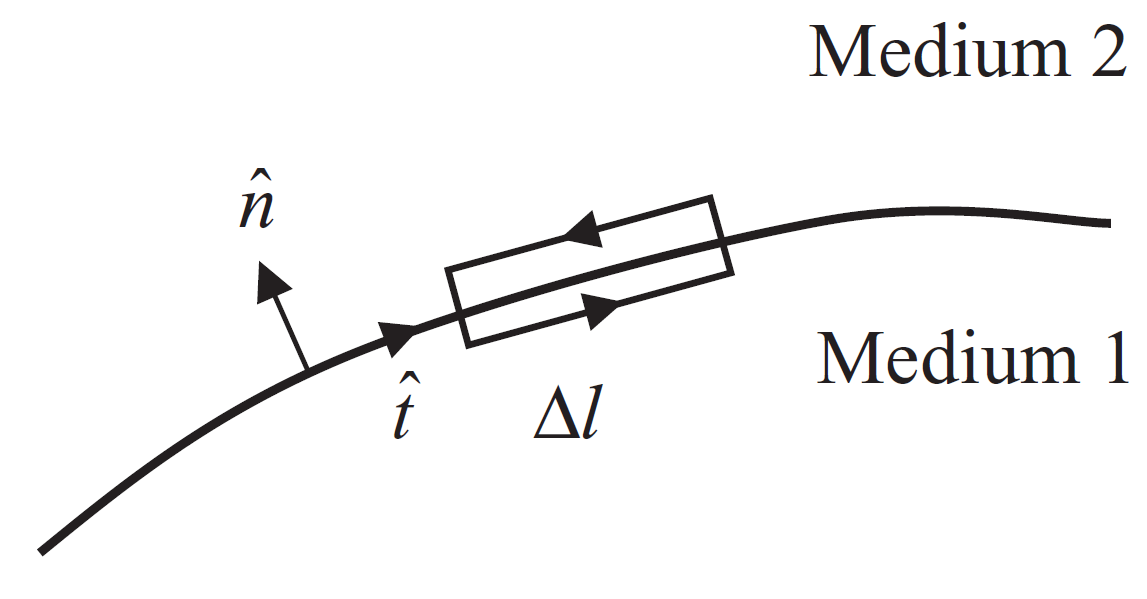
\includegraphics[width=0.25\textwidth]{穿越不连续分界面的矩形框.PNG}
    \caption{穿越不连续分界面的矩形框}
    \label{fig:fig15}
\end{figure}
用$\vec{\mathcal{J}}_s$来表示面电流$(A/m)$,用$\vec{\mathcal{M}}_s$来表示面磁流$(V/m)$。考虑两种不同媒质的分界面,分界面上存在面电流$\vec{\mathcal{J}}_s$,面磁流$\vec{\mathcal{M}}_s$,分界面上的单位法向矢量$\hat{n}$从媒质1指向媒质2,则在分界面上构建一个小矩形,如图\ref{fig:fig15}所示,应用式\ref{eq:eq18}、式\ref{eq:eq19},得
\begin{align}
    \label{eq:eq26}
    \hat{n} \times (\vec{\mathcal{H}}_2-\vec{\mathcal{H}}_1)=\vec{\mathcal{J}}_s \\
    \label{eq:eq27}
    \hat{n} \times (\vec{\mathcal{E}}_2-\vec{\mathcal{E}}_1)=-\vec{\mathcal{M}}_s
\end{align}
式\ref{eq:eq26}表明,磁场强度的切向分量在自由面电流密度不为零的界面两侧是不连续的,式\ref{eq:eq27}表明,电场强度的切向分量在自由面磁流密度不为零的界面两侧是不连续的。
\begin{figure}[ht]
    \centering
    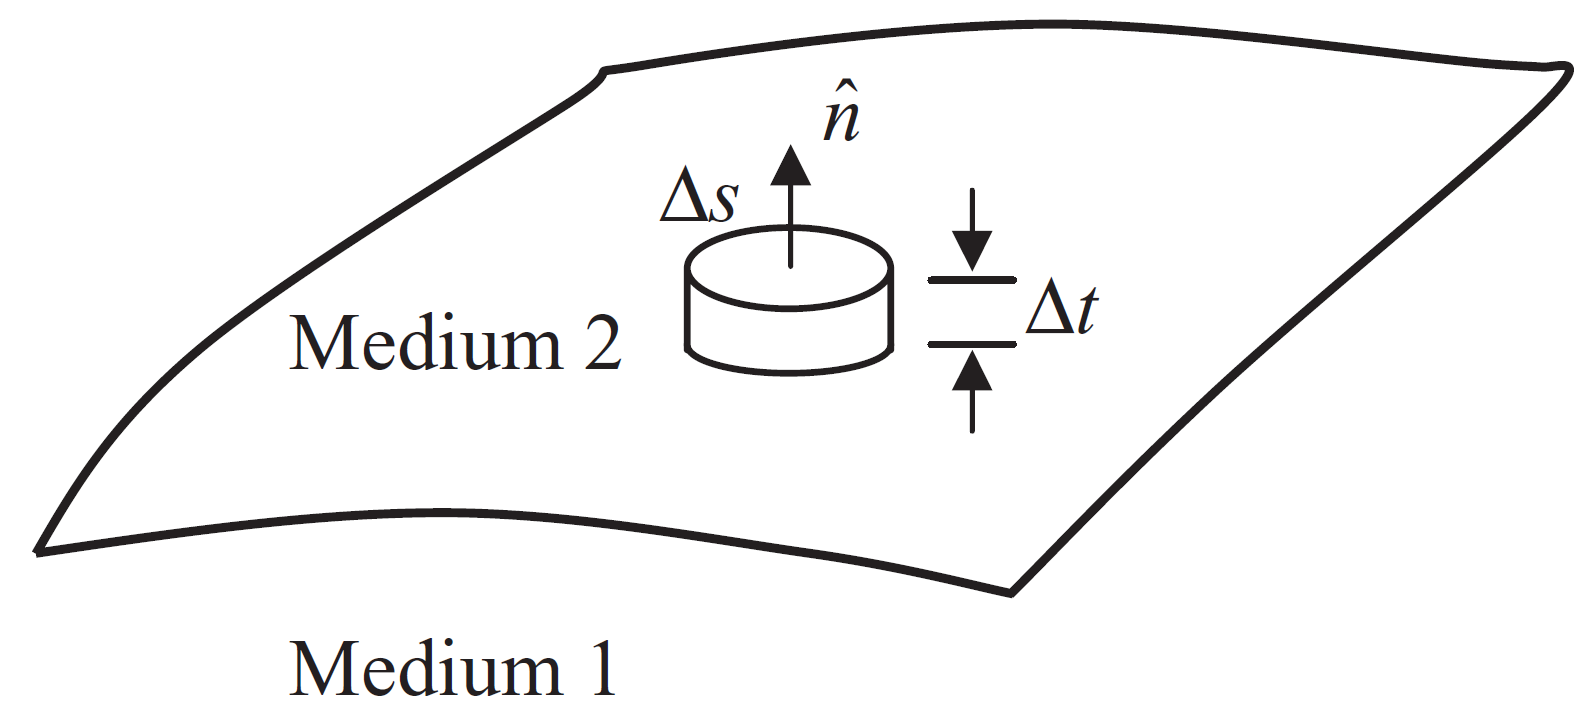
\includegraphics[width=0.35\textwidth]{穿越不连续分界面的扁圆柱.PNG}
    \caption{穿越不连续分界面的扁圆柱}
    \label{fig:fig16}
\end{figure}
\par
用$\varrho _{e,s}$来表示面电荷密度$(C/m^2)$,用$\varrho _{m,s}$来表示面磁荷密度$(Wb/m^2)$。则在分界面上构建一个小圆柱,如图\ref{fig:fig16}所示,应用式\ref{eq:eq20}、式\ref{eq:eq21},得
\begin{align}
    \label{eq:eq28}
    \hat{n} \cdot (\vec{\mathcal{D}}_2-\vec{\mathcal{D}}_1)=\varrho _{e,s} \\
    \label{eq:eq29}
    \hat{n} \cdot (\vec{\mathcal{B}}_2-\vec{\mathcal{B}}_1)=\varrho _{m,s}
\end{align}
式\ref{eq:eq28}表明,电位移矢量的法向分量在面电荷密度不为零的分界面上是不连续的,式\ref{eq:eq29}表明,磁通密度的法向分量在面磁荷密度不为零的分界面上是不连续的。\par
注意:除非是理想导体,电磁场通常不会在分界面上感应出面电荷和面电流,因此,磁场的切向分量和电位移矢量的法向分量在不同媒质的分界面上一般也是连续的。但是,当其中一种媒质是理想电导体(PEC)时,由于其有大量自由电荷,当电磁场加于这种媒质时,自由电荷在电场的作用下移动,直到所产生的方向相反的电场完全抵消外加电场为止,从而在导体表面形成了表面电流和表面电荷。对于理想磁导体(PMC),表面会形成表面磁流和表面电荷。所以,理想导体内部不存在电磁场,即电场和磁场均为0。
\subsection{能量、功率}
考虑介电常数为$\epsilon$、磁导率为$\mu$、电导率为$\sigma $的媒质,用$\vec{\mathcal{J}}_i$、$\vec{\mathcal{M}}_i$表示外加源,将总电流分为外加电流和传导电流,则
\begin{align}
    \label{eq:eq30}
    \nabla \times \vec{\mathcal{E}}&=-\frac{\partial \vec{\mathcal{B}}}{\partial t}-\vec{\mathcal{M}}_i \\
    \label{eq:eq31}
    \nabla \times \vec{\mathcal{H}}&=\frac{\partial \vec{\mathcal{D}}}{\partial t}+\sigma\vec{\mathcal{E}} +\vec{\mathcal{J}}_{i}
\end{align}
有
\begin{align}
    \label{eq:eq32}
    \vec{\mathcal{H}} \cdot (\nabla \times \vec{\mathcal{E}})-\vec{\mathcal{E}} \cdot (\nabla \times \vec{\mathcal{H}})=\nabla \cdot (\vec{\mathcal{E}} \times \vec{\mathcal{H}})=-\vec{\mathcal{E}}\frac{\partial \vec{\mathcal{D}}}{\partial t}-\vec{\mathcal{H}}\frac{\partial \vec{\mathcal{B}}}{\partial t}-\sigma \vec{\mathcal{E}}\cdot \vec{\mathcal{E}}-\vec{\mathcal{E}}\cdot \vec{\mathcal{J}}_i-\vec{\mathcal{H}}\cdot \vec{\mathcal{M}}_i
\end{align}
对上式进行体积分,并应用高斯定理,得
\begin{align}
    \label{eq:eq33}
    \varoiint _S (\vec{\mathcal{E}} \times \vec{\mathcal{H}})\cdot \hat{n}dS+\iiint _V \left(\vec{\mathcal{E}}\frac{\partial \vec{\mathcal{D}}}{\partial t}+\vec{\mathcal{H}}\frac{\partial \vec{\mathcal{B}}}{\partial t}+\sigma \vec{\mathcal{E}}\cdot \vec{\mathcal{E}}+\vec{\mathcal{E}}\cdot \vec{\mathcal{J}}_i+\vec{\mathcal{H}}\cdot \vec{\mathcal{M}}_i\right)dV=0
\end{align}
\par
令
\begin{align}
    \label{eq:eq34}
    \mathcal{P}_e=\varoiint _S (\vec{\mathcal{E}} \times \vec{\mathcal{H}})\cdot \hat{n}dS
\end{align}
重写
\begin{align}
    \label{eq:eq35}
    \vec{\mathcal{E}}\frac{\partial \vec{\mathcal{D}}}{\partial t}=\frac{1}{2}\epsilon \frac{\partial \mathcal{E}^2}{\partial t}=\frac{\partial w_e}{\partial t} \\
    \label{eq:eq36}
    \vec{\mathcal{H}}\frac{\partial \vec{\mathcal{B}}}{\partial t}=\frac{1}{2}\mu \frac{\partial \mathcal{H}^2}{\partial t}=\frac{\partial w_m}{\partial t}
\end{align}
式中,$w_e=\frac{1}{2}\epsilon \mathcal{E}^2$,$w_m=\frac{1}{2}\mu \mathcal{H}^2$代表能量密度$(J/m^3)$,则体积内的总电能和总磁能分别为
\begin{align}
    \label{eq:eq37}
    \mathcal{W}_e=\iiint _V w_e dV =\frac{1}{2}\iiint _V \epsilon\mathcal{E}^2 dV \\
    \label{eq:eq38}
    \mathcal{W}_m=\iiint _V w_m dV =\frac{1}{2}\iiint _V \mu\mathcal{H}^2 dV
\end{align}
空间V内的功率损耗表示为
\begin{align}
    \label{eq:eq39}
    \mathcal{P}_d=\iiint _V \sigma \vec{\mathcal{E}}\cdot \vec{\mathcal{E}} dV=\iiint _V \sigma \mathcal{E}^2 dV
\end{align}
源提供的功率表示为
\begin{align}
    \label{eq:eq40}
    \mathcal{P}_s=-\iiint _V \vec{\mathcal{E}}\cdot \vec{\mathcal{J}}_i+\vec{\mathcal{H}}\cdot \vec{\mathcal{M}}_i dV
\end{align}
则,式\ref{eq:eq33}重写为
\begin{align}
    \label{eq:eq41}
    \mathcal{P}_s=\mathcal{P}_e+\mathcal{P}_d+\frac{\partial}{\partial t}(\mathcal{W}_e+\mathcal{W}_m)
\end{align}
上式为\textbf{\color{blue}{坡印廷定理}},表明源提供的功率等于从闭合曲面流出的功率、空间内消耗的功率和空间内总能量增加的速率之和。
令$p_e=\nabla \cdot (\vec{\mathcal{E}} \times \vec{\mathcal{H}})$,$p_d=\sigma \vec{\mathcal{E}}\cdot \vec{\mathcal{E}}$,$p_s=-(\vec{\mathcal{E}}\cdot \vec{\mathcal{J}}_i+\vec{\mathcal{H}}\cdot \vec{\mathcal{M}}_i)$,得坡印廷定理的微分形式:
\begin{align}
    \label{eq:eq42}
    p_s=p_e+p_d+\frac{\partial}{\partial t}(w_e+w_m)
\end{align}
定义\textbf{\color{blue}{坡印廷矢量}}:
\begin{align}
    \vec{\mathcal{S}}=\vec{\mathcal{E}} \times \vec{\mathcal{H}}
\end{align}
考虑两个瞬时量$\vec{\mathcal{A}}(t)$、$\vec{\mathcal{B}}(t)$,二者的乘积可以表示为
\begin{align}
    \label{eq:eq47}
    \vec{\mathcal{A}}(t)\circ \vec{\mathcal{B}}(t)&=Re[\mathbf{A}(t)e^{jwt}]\circ Re[\mathbf{B}(t)e^{jwt}] \nonumber \\
                                                  &=\frac{1}{2}Re[\mathbf{A} \circ \mathbf{B}^*]+\frac{1}{2}Re[\mathbf{A} \circ \mathbf{B}e^{j2wt}]
\end{align}
对上式取时间平均值,得
\begin{align}
    \overline{\vec{\mathcal{A}}(t)\circ \vec{\mathcal{B}}(t)}=\frac{1}{T}\int_{0}^{T}\vec{\mathcal{A}}(t)\circ \vec{\mathcal{B}}(t) dt =\frac{1}{2}Re[\mathbf{A} \circ \mathbf{B}^*]
\end{align}
式中,$\circ$既可以表示点乘,也可以表示叉乘,$T=2\pi/w$。\par
对坡印廷矢量求时间平均值,有
\begin{align}
    \overline{\vec{\mathcal{S}}(t)}=\overline{\vec{\mathcal{E}}(t) \times \vec{\mathcal{H}}(t)}=\frac{1}{2}Re[\mathbf{E}\times \mathbf{H}^*]=Re(\mathbf{S})
\end{align}
式中$\mathbf{S}=\frac{1}{2}\mathbf{E}\times \mathbf{H}^*$为复数坡印廷矢量。
能量密度的时间平均值为
\begin{align}
    \overline{w_e}=\frac{1}{2}\epsilon \overline{\vec{\mathcal{E}}(t)\cdot \vec{\mathcal{E}}(t)}=\frac{1}{4}\epsilon Re[\mathbf{E}\cdot \mathbf{E}^*] \\
    \overline{w_m}=\frac{1}{2}\mu \overline{\vec{\mathcal{H}}(t)\cdot \vec{\mathcal{H}}(t)}=\frac{1}{4}\mu Re[\mathbf{H}\cdot \mathbf{H}^*]
\end{align}
由式\ref{eq:eq47}得
\begin{align}
    w_e=\frac{1}{2}\epsilon \vec{\mathcal{E}}(t)\cdot \vec{\mathcal{E}}(t)=\frac{1}{4}\epsilon Re[\mathbf{E}\cdot \mathbf{E}^*]+\frac{1}{4}\epsilon Re[\mathbf{E}\cdot \mathbf{E}e^{j2wt}] \\
    w_m=\frac{1}{2}\mu      \vec{\mathcal{H}}(t)\cdot \vec{\mathcal{H}}(t)=\frac{1}{4}\mu      Re[\mathbf{H}\cdot \mathbf{H}^*]+\frac{1}{4}\mu      Re[\mathbf{H}\cdot \mathbf{H}e^{j2wt}]
\end{align}
其时间导数
\begin{align}
    \frac{\partial w_e}{\partial t}=-\frac{w}{2}\epsilon Im[\mathbf{E}\cdot \mathbf{E}e^{j2wt}] \\
    \frac{\partial w_m}{\partial t}=-\frac{w}{2}\mu      Im[\mathbf{H}\cdot \mathbf{H}e^{j2wt}]
\end{align}
故
\begin{align}
    \overline{\frac{\partial w_e}{\partial t}}=0 \\
    \overline{\frac{\partial w_m}{\partial t}}=0
\end{align}
上式表明,虽然瞬时能量密度是不断变化的,但是其时间平均值为零。因此,式\ref{eq:eq42}可重写为
\begin{align}
    \overline{p_s}=\overline{p_e}+\overline{p_d}
\end{align}
上式是时谐场在时间平均意义下的能量守恒定律。\par
从麦克斯韦方程组的复数形式出发,利用式\ref{eq:eq43}与式\ref{eq:eq44},可得
\begin{align}
    \nabla \cdot (\mathbf{E}\times \mathbf{H}^*)=-jw\mu|\mathbf{H}|^2+jw\epsilon |\mathbf{E}|^2-\sigma |\mathbf{E}|^2-\mathbf{H}^*\cdot \mathbf{M}_i-\mathbf{E}\cdot \mathbf{J}_i^*
\end{align}
记$p_e=\frac{1}{2}\nabla \cdot (\mathbf{E}\times \mathbf{H}^*)$、$p_d=\frac{1}{2}\sigma |\mathbf{E}|^2$、$p_s=-\frac{1}{2}(\mathbf{H}^*\cdot \mathbf{M}_i+\mathbf{E}\cdot \mathbf{J}_i^*)$、$w_e=\frac{1}{4}\epsilon |\mathbf{E}|^2$、$w_m=\frac{1}{4}\mu|\mathbf{H}|^2$,则上式重写为
\begin{align}
    p_s=p_e+p_d+j2w(w_m-w_e)
\end{align}
称为复相量的坡印廷定理。
\section{\textsf{自由空间中的电磁辐射}}
\subsection{标量电位、矢量磁位}
由麦克斯韦方程组的复数形式得,在静态场中,$w \to 0$,麦克斯韦方程组重写为
\begin{align}
    \label{eq:eq48}
    \nabla \times \mathbf{E}&=-\mathbf{M} \\
    \label{eq:eq49}
    \nabla \times \mathbf{H}&=\mathbf{J} \\
    \label{eq:eq50}
    \nabla \cdot \mathbf{D}&=\varrho _{e} \\
    \label{eq:eq51}
    \nabla \cdot \mathbf{B}&=\varrho _{m}
\end{align}
\subsubsection{磁流为零,静电场由电荷产生}
根据式\ref{eq:eq48}、式\ref{eq:eq50},有
\begin{align}
    \label{eq:eq52}
    \nabla \times \mathbf{E}&=0 \\
    \label{eq:eq53}
    \nabla \cdot \mathbf{D}&=\varrho _{e}
\end{align}
此时$\mathbf{E}$是一个无旋矢量,可以表示为一个标量函数的梯度,即
\begin{align}
    \label{eq:eq56}
    \mathbf{E}=-\nabla \varphi
\end{align}
其中,$\varphi$称为标量电位,将式\ref{eq:eq56}代入式\ref{eq:eq53},可得
\begin{align}
    \label{eq:eq58}
    \nabla^2\varphi =-\frac{\varrho _{e}}{\epsilon}
\end{align}
上式称为泊松方程,在无限大空间中,其解为
\begin{align}
    \label{eq:eq60}
    \varphi(\vec{r})=\frac{1}{4\pi \epsilon}\iiint_V\frac{\varrho _e(\vec{r}')}{R}dV',\qquad R=|\vec{r}-\vec{r}'|
\end{align}
\subsubsection{磁荷为零,静磁场由电流产生}
根据式\ref{eq:eq49}、式\ref{eq:eq51},有
\begin{align}
    \label{eq:eq54}
    \nabla \times \mathbf{H}&=\mathbf{J} \\
    \label{eq:eq55}
    \nabla \cdot \mathbf{B}&=0
\end{align}
此时$\mathbf{B}$是一个无散矢量,可以表示为一个矢量函数的旋度,即
\begin{align}
    \label{eq:eq57}
    \mathbf{B}=\nabla \times \mathbf{A}
\end{align}
其中,$\mathbf{A}$称为矢量磁位,将式\ref{eq:eq57}代入式\ref{eq:eq54},可得
\begin{align}
    \label{eq:eq59}
    \nabla \times (\nabla \times \mathbf{A})=\nabla(\nabla \cdot \mathbf{A})-\nabla^2\mathbf{A}=\mu \mathbf{J}
\end{align}
令$\mathbf{A}$的散度$\nabla \cdot \mathbf{A}=0$(\textbf{\color{blue}{库仑规范}}),则式\ref{eq:eq59}简化为\footnote{$\mathbf{A}$的散度规定只是为了唯一地确定$\mathbf{A}$,由于$\mathbf{A}$只是一个为了求解$\mathbf{H}$而引入的一个中间变量,它的唯一性并不重要,即使$\mathbf{A}$不是唯一的,通过式\ref{eq:eq57}求得的磁场总是唯一的,因此$\mathbf{A}$的散度并不影响最终的磁场解,因而可以任意规定其值。}
\begin{align}
    \label{eq:eq61}
    \nabla^2\mathbf{A}=-\mu \mathbf{J}
\end{align}
上式称为矢量泊松方程,在无限大空间中,其解为
\begin{align}
    \label{eq:eq62}
    \mathbf{A}(\vec{r})=\frac{\mu}{4\pi}\iiint_V\frac{\mathbf{J}(\vec{r}')}{R}dV',\qquad R=|\vec{r}-\vec{r}'|
\end{align}
\subsection{自由空间中的场-源关系}
在时谐场中,将电场和磁场分解成电流源产生的场和磁流源产生的场,即
\begin{align}
    \label{eq:eq63}
    \mathbf{E}=\mathbf{E}_e+\mathbf{E}_m \qquad \mathbf{H}=\mathbf{H}_e+\mathbf{H}_m
\end{align}
式中,$\mathbf{E}_e$、$\mathbf{H}_e$满足
\begin{align}
    \label{eq:eq64}
    \nabla \times \mathbf{E}_e&=-jw\mu\mathbf{H}_e \\
    \label{eq:eq65}
    \nabla \times \mathbf{H}_e&=jw\epsilon\mathbf{E}_e+\mathbf{J} \\
    \label{eq:eq66}
    \nabla \cdot (\epsilon\mathbf{E}_e)&=\varrho _{e} \\
    \label{eq:eq67}
    \nabla \cdot (\mu\mathbf{H}_e)&=0
\end{align}
$\mathbf{E}_e$、$\mathbf{H}_e$满足
\begin{align}
    \label{eq:eq68}
    \nabla \times \mathbf{E}_m&=-jw\mu\mathbf{H}_m-\mathbf{M} \\
    \label{eq:eq69}
    \nabla \times \mathbf{H}_m&=jw\epsilon\mathbf{E}_m \\
    \label{eq:eq70}
    \nabla \cdot (\epsilon\mathbf{E}_m)&=0 \\
    \label{eq:eq71}
    \nabla \cdot (\mu\mathbf{H}_m)&=\varrho _{m}
\end{align}
由上可知,$\mathbf{B}_e=\mu\mathbf{H}_e$、$\mathbf{D}_m=\epsilon\mathbf{E}_m$是无散矢量,则令
\begin{align}
    \label{eq:eq72}
    \mathbf{B}_e&=\nabla \times \mathbf{A} \\
    \label{eq:eq73}
    \mathbf{D}_m&=-\nabla \times \mathbf{F}
\end{align}
其中$\mathbf{A}$是矢量磁位,$\mathbf{F}$是矢量电位,分别代入式\ref{eq:eq64}和式\ref{eq:eq69},有
\begin{align}
    \label{eq:eq74}
    \nabla \times (\mathbf{E}_e+jw\mathbf{A})=0 \\
    \label{eq:eq75}
    \nabla \times (\mathbf{D}_m+jw\mathbf{F})=0
\end{align}
引入标量电位$\varphi$和标量磁位$\psi$,有
\begin{align}
    \label{eq:eq76}
    \mathbf{E}_e+jw\mathbf{A}=-\nabla \varphi \\
    \label{eq:eq77}
    \mathbf{D}_m+jw\mathbf{F}=-\nabla \psi
\end{align}
分别将式\ref{eq:eq72}、式\ref{eq:eq76}代入式\ref{eq:eq65},式\ref{eq:eq73}、式\ref{eq:eq77}代入式\ref{eq:eq68},得
\begin{align}
    \label{eq:eq78}
    \nabla \times (\frac{1}{\mu}\nabla\times \mathbf{A})=-jw\epsilon \nabla \varphi+w^2\epsilon\mathbf{A}+\mathbf{J} \\
    \label{eq:eq79}
    -\nabla \times (\frac{1}{\epsilon}\nabla\times \mathbf{F})=jw\mu \nabla \psi-w^2\mu\mathbf{F}-\mathbf{M}
\end{align}
利用等式$\nabla\times(\nabla\times\mathbf{A})=\nabla(\nabla \cdot\mathbf{A})-\nabla^2\mathbf{A}$、$\nabla\times(\nabla\times\mathbf{F})=\nabla(\nabla \cdot\mathbf{F})-\nabla^2\mathbf{F}$,且令$\mathbf{A}$的散度$\nabla\cdot\mathbf{A}=-jw\epsilon\mu\varphi$,令$\mathbf{F}$的散度$\nabla\cdot\mathbf{F}=-jw\epsilon\mu\psi$(\textbf{\color{blue}{洛伦兹规范}}),$k^2=w^2\epsilon\mu$,得\footnote{$k$是波数,它与波长$\lambda$的关系为$k=\frac{2\pi}{\lambda}$,场在媒质中的传播速度$c=\frac{1}{\sqrt{\mu\epsilon}}$}
\begin{align}
    \label{eq:eq80}
    \nabla^2\mathbf{A}+k^2\mathbf{A}=-\mu\mathbf{J} \\
    \label{eq:eq81}
    \nabla^2\mathbf{F}+k^2\mathbf{F}=-\epsilon\mathbf{M}
\end{align}
上式称为\textbf{\color{blue}{矢量亥姆霍兹方程}}。通过求解矢量亥姆霍兹方程,得到矢量磁位$\mathbf{A}$、矢量电位$\mathbf{F}$后,分别代入式\ref{eq:eq72}、式\ref{eq:eq76},式\ref{eq:eq73}、式\ref{eq:eq77},并结合洛伦兹规范,可得
\begin{align}
    \mathbf{E}_e&=-jw\mathbf{A}+\frac{1}{jw\mu\epsilon}\nabla(\nabla \cdot \mathbf{A}) \\
    \mathbf{H}_e&=\frac{1}{\mu}\nabla\times\mathbf{A} \\
    \mathbf{E}_m&=-\frac{1}{\epsilon}\nabla\times\mathbf{F} \\
    \mathbf{H}_m&=-jw\mathbf{F}+\frac{1}{jw\mu\epsilon}\nabla(\nabla \cdot \mathbf{F})
\end{align}
代入式\ref{eq:eq63},有
\begin{align}
    \label{eq:eq82}
    \mathbf{E}&=-jw\mathbf{A}+\frac{1}{jw\mu\epsilon}\nabla(\nabla \cdot \mathbf{A})-\frac{1}{\epsilon}\nabla\times\mathbf{F} \\
    \label{eq:eq83}
    \mathbf{H}&=-jw\mathbf{F}+\frac{1}{jw\mu\epsilon}\nabla(\nabla \cdot \mathbf{F})+\frac{1}{\mu}\nabla\times\mathbf{A}
\end{align}
\par
由于式\ref{eq:eq80}和式\ref{eq:eq81}是线性的,且形式相同,因此将它们的解表示成点源解的线性叠加,即
\begin{align}
    \label{eq:eq84}
    \mathbf{A}(\vec{r})&=\mu\iiint_V\mathbf{J}(\vec{r}')G(\vec{r},\vec{r}')dV' \\
    \label{eq:eq97}
    \mathbf{F}(\vec{r})&=\epsilon\iiint_V\mathbf{M}(\vec{r}')G(\vec{r},\vec{r}')dV'
\end{align}
式中,$G(\vec{r},\vec{r}')$是对应于点源的基本解(\textbf{\color{blue}{格林函数}})。引入\textbf{\color{blue}{$\delta$函数}}:
\begin{align}
    \label{eq:eq85}
    \delta(\vec{r}-\vec{r}')&=
    \left\{
        \begin{array}{lr}
            \infty, &\vec{r}=\vec{r}' \\
            0,      &\vec{r}\neq\vec{r}'
        \end{array}
    \right. \\
    \label{eq:eq86}
    \iiint_V\delta(\vec{r}-\vec{r}')dV&=
    \left\{
        \begin{array}{lr}
            1, &\vec{r}'\in V \\
            0, &\vec{r}'\notin V
        \end{array}
    \right.
\end{align}
对于任意在$\vec{r}'$连续的函数,有
\begin{align}
    \label{eq:eq87}
    \iiint_Vf(\vec{r})\delta(\vec{r}-\vec{r}')dV=
    \left\{
        \begin{array}{lr}
            f(\vec{r}'), &\vec{r}'\in V \\
            0, &\vec{r}'\notin V
        \end{array}
    \right.
\end{align}
在笛卡尔坐标系、柱坐标系、球坐标系中,三维$\delta$函数和一维$\delta$函数的关系为
\begin{align}
    \delta(\vec{r}-\vec{r}')=\delta(x-x')\delta(y-y')\delta(z-z') \\
    \delta(\vec{r}-\vec{r}')=\frac{\delta(\rho-\rho')\delta(\phi-\phi')\delta(z-z')}{\rho} \\
    \delta(\vec{r}-\vec{r}')=\frac{\delta(r-r')\delta(\theta-\theta')\delta(\phi-\phi')}{r^2\sin\theta}
\end{align}
则电流源$\mathbf{J}$、磁流源$\mathbf{M}$可以表示成点源的线性叠加:
\begin{align}
    \label{eq:eq88}
    \mathbf{J}(\vec{r})&=\iiint_V\mathbf{J}(\vec{r}')\delta(\vec{r}-\vec{r}')dV' \\
    \label{eq:eq98}
    \mathbf{M}(\vec{r})&=\iiint_V\mathbf{M}(\vec{r}')\delta(\vec{r}-\vec{r}')dV'
\end{align}
将式\ref{eq:eq84}和式\ref{eq:eq88}代入式\ref{eq:eq80},并将式\ref{eq:eq97}和式\ref{eq:eq98}代入式\ref{eq:eq81},得
\begin{align}
    \label{eq:eq89}
    \iiint_V[\nabla^2G(\vec{r},\vec{r}')+k^2G(\vec{r},\vec{r}')]\mathbf{J}(\vec{r}')dV'&=-\iiint_V\mathbf{J}(\vec{r}')\delta(\vec{r}-\vec{r}')dV' \\
    \label{eq:eq99}
    \iiint_V[\nabla^2G(\vec{r},\vec{r}')+k^2G(\vec{r},\vec{r}')]\mathbf{M}(\vec{r}')dV'&=-\iiint_V\mathbf{M}(\vec{r}')\delta(\vec{r}-\vec{r}')dV'
\end{align}
上式对任意$\mathbf{J}(\vec{r}')$、$\mathbf{M}(\vec{r}')$都成立,因此有
\begin{align}
    \label{eq:eq90}
    \nabla^2G(\vec{r},\vec{r}')+k^2G(\vec{r},\vec{r}')=-\delta(\vec{r}-\vec{r}')
\end{align}
\par
记$G_0(\vec{r},\vec{r}')$是自由空间中的格林函数,先考虑$\vec{r}'=0$的特殊情况,此时$G_0(\vec{r},0)$关于坐标原点球对称。
代入式\ref{eq:eq90},有
\begin{align}
    \label{eq:eq91}
    \frac{1}{r^2}\frac{d}{dr}\left[r^2\frac{dG_0(\vec{r},0)}{dr}\right]+k^2G_0(\vec{r},0)=-\delta(\vec{r}-0)
\end{align}
对于$\vec{r}\neq 0$,上式写成
\begin{align}
    \label{eq:eq92}
    \frac{d^2[rG_0(\vec{r},0)]}{dr^2}+k^2[rG_0(\vec{r},0)]=0
\end{align}
该方程有两个独立解:
\begin{align}
    \label{eq:eq93}
    rG_0(\vec{r},0)=Ce^{\pm jkr}
\end{align}
式中,$C$为待定常数,$e^{-jkr}$的时域形式为$\cos(wt-kr)$,表示从源点向外传播的波,$e^{jkr}$的时域形式为$\cos(wt+kr)$,表示从无穷远处向源点传播的波,没有物理意义。因此,只取解
\begin{align}
    \label{eq:eq94}
    rG_0(\vec{r},0)=Ce^{-jkr}
\end{align}
将上式代入式\ref{eq:eq91}中,并对其在以$\vec{r}=0$为中心得小球上进行体积分,并令小球半径趋于0,得到待定常数$C=1/4\pi$,故
\begin{align}
    \label{eq:eq95}
    G_0(\vec{r},0)=\frac{e^{-jkr}}{4\pi r}
\end{align}
对于$\vec{r}'\neq0$的情况,从$\vec{r}'$到观察点$\vec{r}$的距离为$|\vec{r}-\vec{r}'|$,因此,
\begin{align}
    \label{eq:eq96}
    G_0(\vec{r},\vec{r}')=\frac{e^{-jk|\vec{r}-\vec{r}'|}}{4\pi |\vec{r}-\vec{r}'|}
\end{align}
上式称为自由空间的标量格林函数,它代表从$\vec{r}'$点发出的向外传播的球面波,分别代入式\ref{eq:eq84}、式\ref{eq:eq97},得矢量磁位$\mathbf{A}$、矢量电位$\mathbf{F}$的解为
\begin{align}
    \label{eq:eq100}
    \mathbf{A}(\vec{r})&=\frac{\mu}{4\pi}\iiint_V\mathbf{J}(\vec{r}')\frac{e^{-jkR}}{R}dV',\qquad R=|\vec{r}-\vec{r}'| \\
    \label{eq:eq101}
    \mathbf{F}(\vec{r})&=\frac{\epsilon}{4\pi}\iiint_V\mathbf{M}(\vec{r}')\frac{e^{-jkR}}{R}dV',\qquad R=|\vec{r}-\vec{r}'|
\end{align}
通过傅里叶变化,得到矢量位的时域表达式:
\begin{align}
    \label{eq:eq102}
    \vec{\mathcal{A}}(\vec{r},t)&=\frac{\mu}{4\pi}\iiint_V\frac{\vec{\mathcal{J}}(\vec{r}',t-R/c)}{R}dV' \\
    \label{eq:eq103}
    \vec{\mathcal{F}}(\vec{r},t)&=\frac{\epsilon}{4\pi}\iiint_V\frac{\vec{\mathcal{M}}(\vec{r}',t-R/c)}{R}dV'
\end{align}
式\ref{eq:eq82}、式\ref{eq:eq83}在时域中表示为
\begin{align}
    \label{eq:eq104}
    \vec{\mathcal{E}}(\vec{r},t)&=-\frac{\partial \vec{\mathcal{A}}(\vec{r},t)}{\partial t}+\frac{1}{\mu\epsilon}\int^{t-R/c}_0\nabla[\nabla\cdot\vec{\mathcal{A}}(\vec{r},\tau)]d\tau-\frac{1}{\epsilon}\nabla\times\vec{\mathcal{F}}(\vec{r},t) \\
    \label{eq:eq105}
    \vec{\mathcal{H}}(\vec{r},t)&=-\frac{\partial \vec{\mathcal{F}}(\vec{r},t)}{\partial t}+\frac{1}{\mu\epsilon}\int^{t-R/c}_0\nabla[\nabla\cdot\vec{\mathcal{F}}(\vec{r},\tau)]d\tau-\frac{1}{\mu}\nabla\times\vec{\mathcal{F}}(\vec{r},t)
\end{align}
式\ref{eq:eq100}、式\ref{eq:eq101}、式\ref{eq:eq82}、式\ref{eq:eq83}给出了频域中的场-源关系,式\ref{eq:eq102}、式\ref{eq:eq103}、式\ref{eq:eq104}、式\ref{eq:eq105}给出了时域中由瞬态源求解瞬态场的方法。
\par
将式\ref{eq:eq100}、式\ref{eq:eq101}代入式\ref{eq:eq82}、式\ref{eq:eq83},交换积分和微分的顺序,得
\begin{align}
    \label{eq:eq106}
    \mathbf{E}(\vec{r})&=-jw\mathbf{A}(\vec{r})+\frac{1}{jw\mu\epsilon}\nabla(\nabla \cdot \mathbf{A}(\vec{r}))-\frac{1}{\epsilon}\nabla\times\mathbf{F}(\vec{r}) \nonumber \\
                       &=-jw\mu\iiint_V\mathbf{J}(\vec{r}')G_0(\vec{r},\vec{r}')dV'+\frac{1}{jw\mu\epsilon}\nabla\left[\nabla \cdot \mu\iiint_V\mathbf{J}(\vec{r}')G_0(\vec{r},\vec{r}')dV'\right] \nonumber \\
                       &\qquad-\frac{1}{\epsilon}\nabla\times\epsilon\iiint_V\mathbf{M}(\vec{r}')G_0(\vec{r},\vec{r}')dV' \nonumber \\
                       &=-jw\mu\iiint_V\left[G_0(\vec{r},\vec{r}')\mathbf{J}(\vec{r}')+\frac{1}{k^2}\nabla\nabla G_0(\vec{r},\vec{r}') \cdot \mathbf{J}(\vec{r}')\right]dV' \nonumber \\
                       &\qquad-\iiint_V\nabla G_0(\vec{r},\vec{r}')\times \mathbf{M}(\vec{r}')dV' \\
    \label{eq:eq107}
    \mathbf{H}(\vec{r})&=-jw\mathbf{F}(\vec{r})+\frac{1}{jw\mu\epsilon}\nabla(\nabla \cdot \mathbf{F}(\vec{r}))+\frac{1}{\mu}\nabla\times\mathbf{A}(\vec{r}) \nonumber \\
                       &=-jw\epsilon\iiint_V\mathbf{M}(\vec{r}')G_0(\vec{r},\vec{r}')dV'+\frac{1}{jw\mu\epsilon}\nabla\left[\nabla \cdot \epsilon\iiint_V\mathbf{M}(\vec{r}')G_0(\vec{r},\vec{r}')dV'\right] \nonumber \\
                       &\qquad+\frac{1}{\mu}\nabla\times\mu\iiint_V\mathbf{J}(\vec{r}')G_0(\vec{r},\vec{r}')dV' \nonumber \\
                       &=-jw\epsilon\iiint_V\left[G_0(\vec{r},\vec{r}')\mathbf{M}(\vec{r}')+\frac{1}{k^2}\nabla\nabla G_0(\vec{r},\vec{r}') \cdot \mathbf{M}(\vec{r}')\right]dV' \nonumber \\
                       &\qquad+\iiint_V\nabla G_0(\vec{r},\vec{r}')\times \mathbf{J}(\vec{r}')dV'
\end{align}
定义$\overline{\mathbf{I}}=\hat{x}\hat{x}+\hat{y}\hat{y}+\hat{z}\hat{z}$为\textbf{\color{blue}{单位并矢}},有$\overline{\mathbf{I}}\cdot\vec{a}=\vec{a}$,$\vec{a}\times\overline{\mathbf{I}}=\vec{a}$。令
\begin{align}
    \label{eq:eq108}
    \overline{\mathbf{G}}_{e0}(\vec{r},\vec{r}')&=\left(\overline{\mathbf{I}}+\frac{1}{k^2}\nabla\nabla\right)G_0(\vec{r},\vec{r}') \\
    \label{eq:eq109}
    \overline{\mathbf{G}}_{m0}(\vec{r},\vec{r}')&=\nabla G_0(\vec{r},\vec{r}')\times \overline{\mathbf{I}}
\end{align}
称$\overline{\mathbf{G}}_{e0}$为\textbf{\color{blue}{自由空间电并矢格林函数}},$\overline{\mathbf{G}}_{m0}$为\textbf{\color{blue}{自由空间磁并矢格林函数}}。代入式\ref{eq:eq106}、式\ref{eq:eq107}得
\begin{align}
    \label{eq:eq110}
    \mathbf{E}(\vec{r})&=-jw\mu\iiint_V\overline{\mathbf{G}}_{e0}(\vec{r},\vec{r}')\cdot \mathbf{J}(\vec{r}')dV'-\iiint_V\overline{\mathbf{G}}_{m0}(\vec{r},\vec{r}')\cdot \mathbf{M}(\vec{r}')dV' \\
    \label{eq:eq111}
    \mathbf{H}(\vec{r})&=-jw\epsilon\iiint_V\overline{\mathbf{G}}_{e0}(\vec{r},\vec{r}')\cdot \mathbf{M}(\vec{r}')dV'+\iiint_V\overline{\mathbf{G}}_{m0}(\vec{r},\vec{r}')\cdot \mathbf{J}(\vec{r}')dV'
\end{align}
分别将$\overline{\mathbf{G}}_{e0}(\vec{r},\vec{r}')$、$\overline{\mathbf{G}}_{m0}(\vec{r},\vec{r}')$写成张量的形式:
\begin{align}
    \label{eq:eq112}
    \overline{\mathbf{G}}_{e0}(\vec{r},\vec{r}')&={\mathbf{G}}_{e0,x}(\vec{r},\vec{r}')\hat{x}+{\mathbf{G}}_{e0,y}(\vec{r},\vec{r}')\hat{y}+{\mathbf{G}}_{e0,y}(\vec{r},\vec{r}')\hat{z} \\
    \label{eq:eq113}
    \overline{\mathbf{G}}_{m0}(\vec{r},\vec{r}')&={\mathbf{G}}_{m0,x}(\vec{r},\vec{r}')\hat{x}+{\mathbf{G}}_{m0,y}(\vec{r},\vec{r}')\hat{y}+{\mathbf{G}}_{m0,y}(\vec{r},\vec{r}')\hat{z}
\end{align}
则${\mathbf{G}}_{e0,u}(\vec{r},\vec{r}')$代表由位于$\vec{r}'$处的$\hat{u}$方向无限小电流源在$\vec{r}$处产生的电场,${\mathbf{G}}_{m0,u}(\vec{r},\vec{r}')$代表由位于$\vec{r}'$处的$\hat{u}$方向无限小电流源在$\vec{r}$处产生的磁场。
\subsection{远场条件和索末菲辐射条件}
在大多实际应用中,只对远场感兴趣,考虑空间几何关系如图\ref{fig:fig0}所示。\par
\begin{figure}[ht]
    \centering
    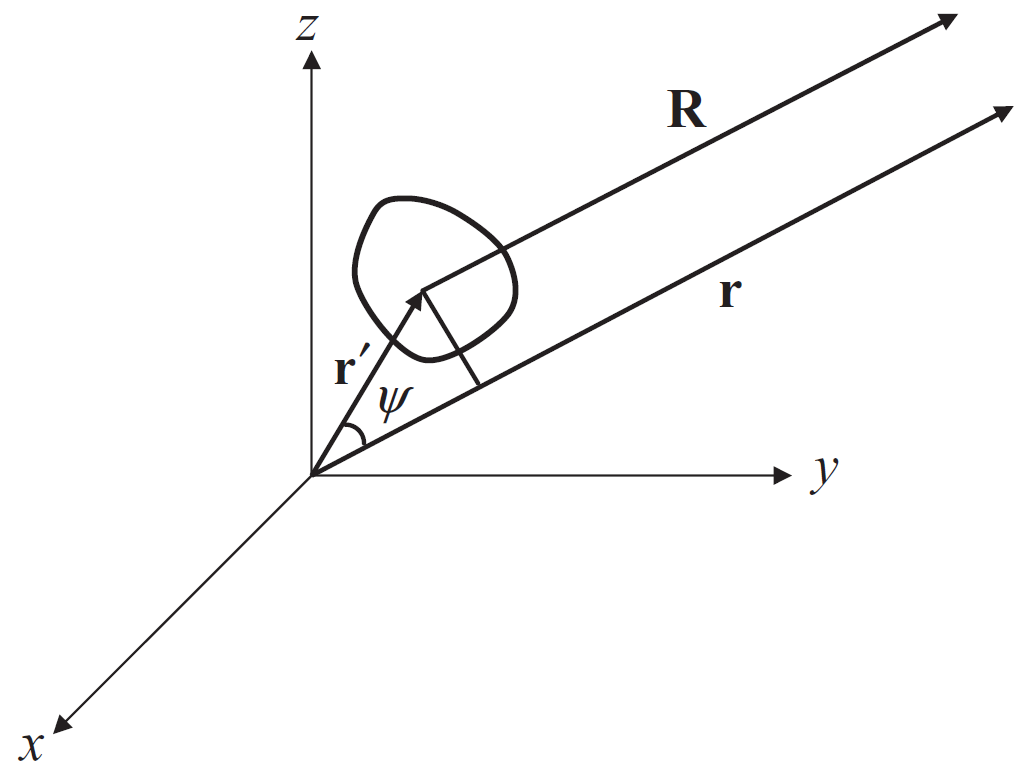
\includegraphics[width=0.4\textwidth]{远场条件.PNG}
    \caption{对于远场区的观察点,$\mathbf{R}$和$\vec{r}$几乎相互平行}
    \label{fig:fig0}
\end{figure}
在远场条件下,$R\gg \lambda$,$r\gg r'$,记$\vec{r}$与$\vec{r}'$之间的夹角为$\psi $,则有
\begin{align}
    \label{eq:eq114}
    R=|\vec{r}-\vec{r}'|&=\sqrt{r^2+r'^2-2rr'\cos \psi} \nonumber \\
                        &\approx r-r'\cos \psi
\end{align}
将上式代入式\ref{eq:eq100}、式\ref{eq:eq101}中,
\begin{align}
    \label{eq:eq115}
    \mathbf{A}&=\frac{\mu}{4\pi r}e^{-jkr}\mathbf{N} \\
    \label{eq:eq116}
    \mathbf{F}&=\frac{\epsilon}{4\pi r}e^{-jkr}\mathbf{L}
\end{align}
式中,
\begin{align}
    \label{eq:eq117}
    \mathbf{N}=\iiint_V\mathbf{J}e^{jkr'\cos\psi}dV' \\
    \label{eq:eq118}
    \mathbf{L}=\iiint_V\mathbf{M}e^{jkr'\cos\psi}dV'
\end{align}
其中,
\begin{align}
    \label{eq:eq121}
    r'\cos\psi=\vec{r}'\cdot\hat{r}=\vec{r}'\cdot\hat{x}\sin\theta\cos\phi+\vec{r}'\cdot\hat{y}\sin\theta\sin\phi+\vec{r}'\cdot\hat{z}\cos\theta
\end{align}
代入式\ref{eq:eq82}、式\ref{eq:eq83},只保留主要项,得到远场为:
\begin{align}
    \label{eq:eq119}
    \mathbf{E}&\approx\frac{jk}{4\pi r}e^{-jkr}\left[\hat{r}\times\mathbf{L}-\eta\left(\mathbf{N}-\hat{r}N_r\right)\right] \nonumber \\
              &=-\frac{jk}{4\pi r}e^{-jkr}\left[\hat{\theta}\left(L_{\phi}+\eta N_{\theta}\right)-\hat{\phi}\left(L_{\theta}-\eta N_{\phi}\right)\right] \\
    \label{eq:eq120}
    \mathbf{H}&\approx-\frac{jk}{4\pi r}e^{-jkr}\left[\hat{r}\times\mathbf{N}+\frac{1}{\eta}\left(\mathbf{L}-\hat{r}L_r\right)\right] \nonumber \\
              &=-\frac{jk}{4\pi r}e^{-jkr}\frac{1}{\eta}\left[\hat{\theta}\left(L_{\theta}-\eta N_{\phi}\right)+\hat{\phi}\left(L_{\phi}+\eta N_{\theta}\right)\right]
\end{align}
其中$\eta=\sqrt{\mu/\epsilon}$。由上式可知,远场相对于$\hat{r}$方向是横电磁场。进一步计算坡印廷矢量为:
\begin{align}
    \label{eq:eq122}
    \mathbf{S}&=\frac{1}{2}\mathbf{E}\times\mathbf{H}^* \nonumber \\
              &=\hat{r}\left(\frac{k}{4\pi r}\right)^2\left[\frac{1}{\eta}\left(\left|L_{theta}\right|^2+\left|L_{phi}\right|^2\right)+\eta\left(\left|N_{theta}\right|^2+\left|N_{phi}\right|^2\right)+2Re\left(L_{\phi}N_{\theta}^*-L_{\theta}N_{\phi}^*\right)\right]
\end{align}
上式说明,虽然两种源产生的总场是每种源产生的场的线性叠加,但其功率密度不是线性叠加的关系,因为还含有交叉项。由式\ref{eq:eq119}、式\ref{eq:eq120}可知,
\begin{align}
    \label{eq:eq123}
    \hat{r}\times\mathbf{E}=-\frac{jk}{4\pi r}e^{-jkr}\left[\left(\mathbf{L}-\hat{r}L_r\right)+\eta\left(\hat{r}\times\mathbf{N}\right)\right]=\eta\mathbf{H}
\end{align}
由上式可得\textbf{\color{blue}{索末菲辐射条件}}:
\begin{align}
    \label{eq:eq124}
    \lim_{r\to\infty}r(\nabla\times\mathbf{E}+jk\hat{r}\times\mathbf{E})&=0 \\
    \label{eq:eq125}
    \lim_{r\to\infty}r(\nabla\times\mathbf{H}+jk\hat{r}\times\mathbf{H})&=0
\end{align}
上式表明:\\
(1)在离开源的远处,场只能从源向远处传播;\\
(2)电场和磁场对传播方向来说是横向的,并且互相正交;\\
(3)电场和磁场的幅度比值固定,等于$\eta$。
\subsection{不同源的远场表达}
\subsubsection{无限小电偶极子}
\begin{figure}[ht]
    \centering
    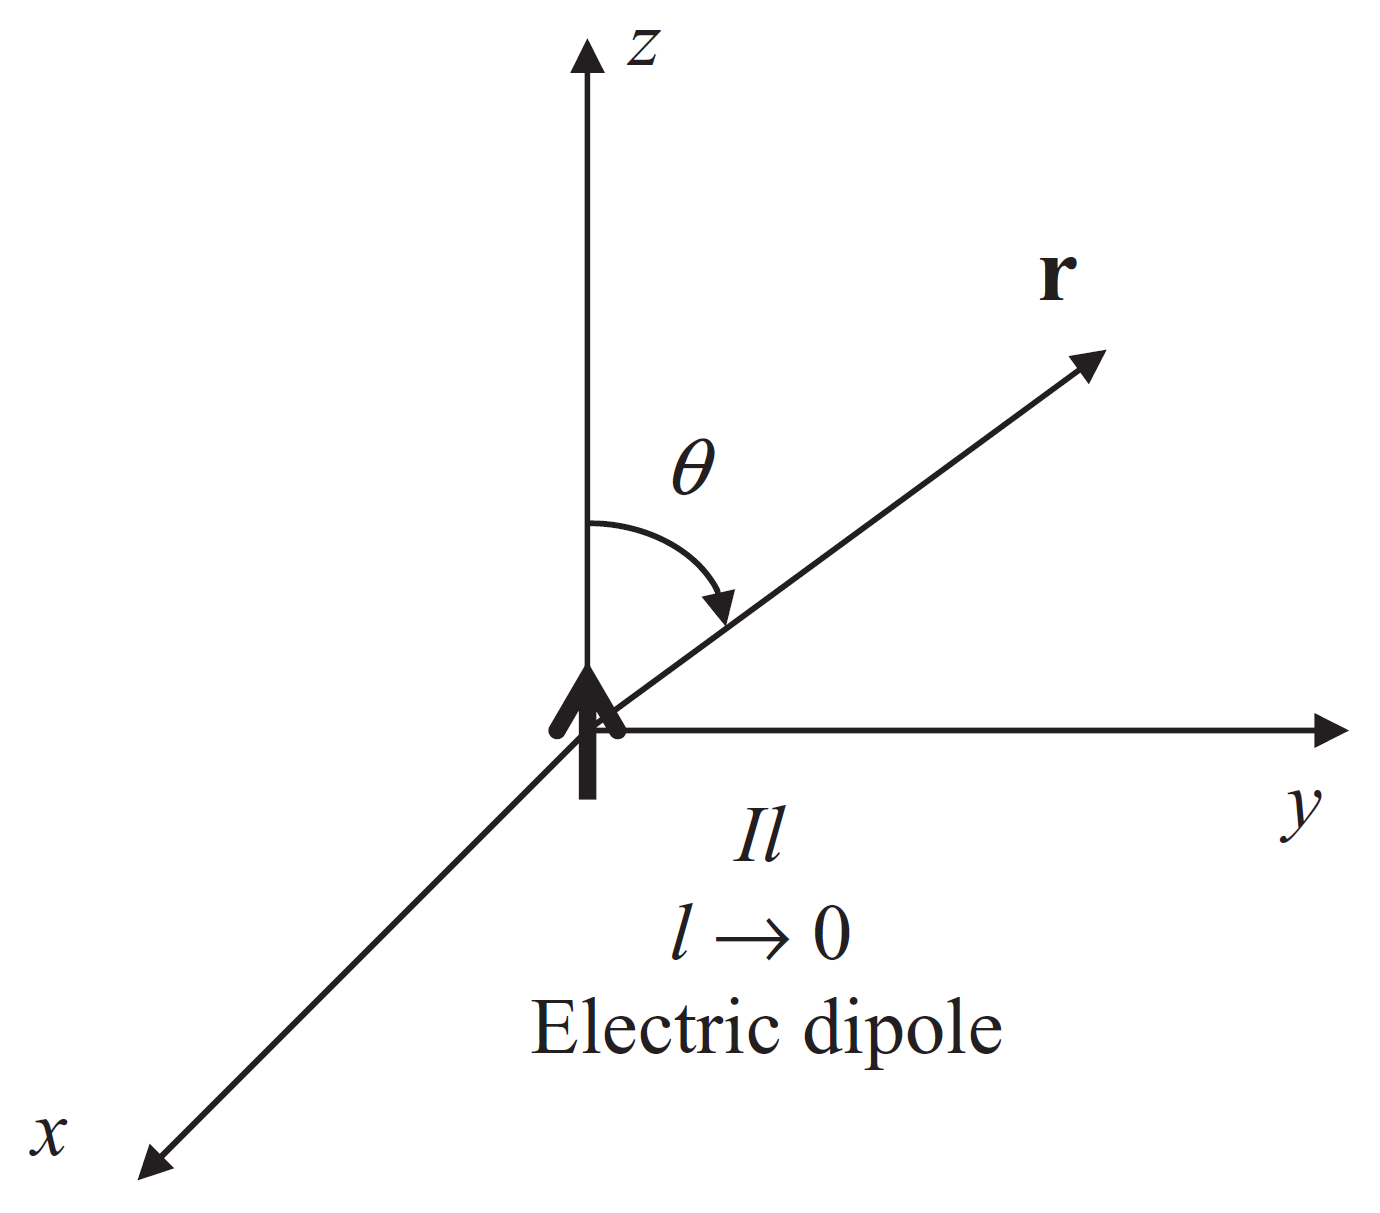
\includegraphics[width=0.35\textwidth]{无限小电偶极子.PNG}
    \caption{无限小电偶极子}
    \label{fig:fig1}
\end{figure}
考虑一个非常短的线电流,长度为$l$,时谐电流为$I$,如图\ref{fig:fig1}所示。则在远场区,
\begin{align}
    \label{eq:eq126}
    E_{\theta}&\approx\frac{jk\eta Il\sin\theta}{4\pi r}e^{-jkr} \\
    \label{eq:eq127}
    H_{\phi}&\approx\frac{jkIl\sin\theta}{4\pi r}e^{-jkr}
\end{align}
其能流密度为
\begin{align}
    \label{eq:eq128}
    \mathbf{S}=\frac{1}{2}\mathbf{E}\times\mathbf{H}^*=\hat{r}\frac{\eta}{2}\left|\frac{kIl\sin\theta}{4\pi r}\right|^2
\end{align}
对坡印廷矢量在半径为$r$的球面上积分,得到流出的复功率为
\begin{align}
    \label{eq:eq129}
    P_e=\frac{1}{2}\varoiint_S(\mathbf{E}\times\mathbf{H}^*)=\eta\frac{\pi}{3}\left|\frac{Il}{\lambda}\right|^2\left[1-\frac{j}{(kr)^3}\right]
\end{align}
其实部为辐射功率的时均值,
\begin{align}
    \label{eq:eq130}
    Re(P_e)=\eta\frac{\pi}{3}\left|\frac{Il}{\lambda}\right|^2
\end{align}
考虑半径为$a$和$b(b>a)$的两个球面之间区域内的无功功率:
\begin{align}
    \label{eq:eq131}
    2w(W_m-W_e)=\eta\frac{\pi}{3}\left|\frac{Il}{\lambda}\right|^2\left[\frac{1}{(kb)^3}-\frac{1}{(ka)^3}\right]
\end{align}
因此,电偶极子周围的电场能量时均值总是大于磁场能量的时均值。
\subsubsection{有限长电偶极子}
\begin{figure}[ht]
    \centering
    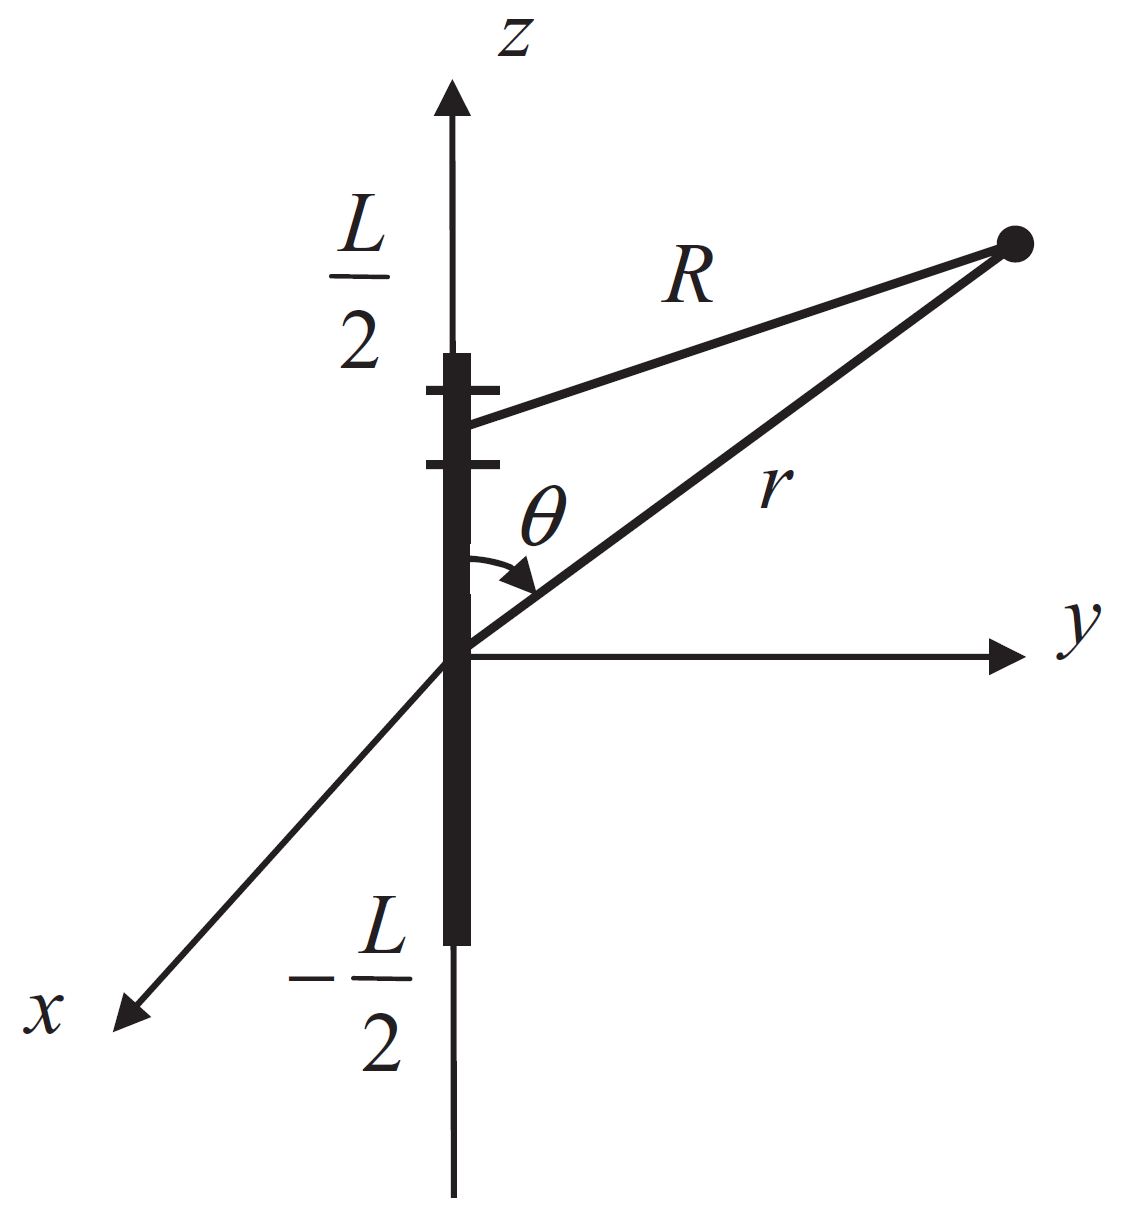
\includegraphics[width=0.3\textwidth]{有限长电偶极子.PNG}
    \caption{有限长电偶极子}
    \label{fig:fig2}
\end{figure}
考虑一个有限长的线电流,长度为$L$,如图\ref{fig:fig2}所示。假设其上电流已知,
\begin{align}
    \label{eq:eq132}
    I(z)=I_0\sin\left[k\left(\frac{L}{2}-\left|z\right|\right)\right]
\end{align}
式中,$I_0$是常数。则在远场区,
\begin{align}
    \label{eq:eq133}
    E_{\theta}&\approx\frac{j\eta I_0}{2\pi r}e^{-jkr}\frac{\cos\left(k\frac{L}{2}\cos\theta\right)-\cos\left(k\frac{L}{2}\right)}{k\sin^2\theta} \\
    \label{eq:eq134}
    H_{\phi}&\approx\frac{jI_0}{2\pi r}e^{-jkr}\frac{\cos\left(k\frac{L}{2}\cos\theta\right)-\cos\left(k\frac{L}{2}\right)}{k\sin^2\theta}
\end{align}
上式表明,当偶极子长度增加时,辐射功率更加向$\theta=\pi /2$集中,方向性更强,当长度超过一个波长时,辐射波束开始分裂,此时偶极子上的电流不再沿一个方向流动,导致向$\theta=\pi /2$的辐射减小,而向其他方向的辐射增加。
\par
一般情况下,偶极子上的电流分布是未知的,需要用特殊的数值方法求解边值问题得到。
\subsubsection{圆电流环(磁偶极子)}
\begin{figure}[ht]
    \centering
    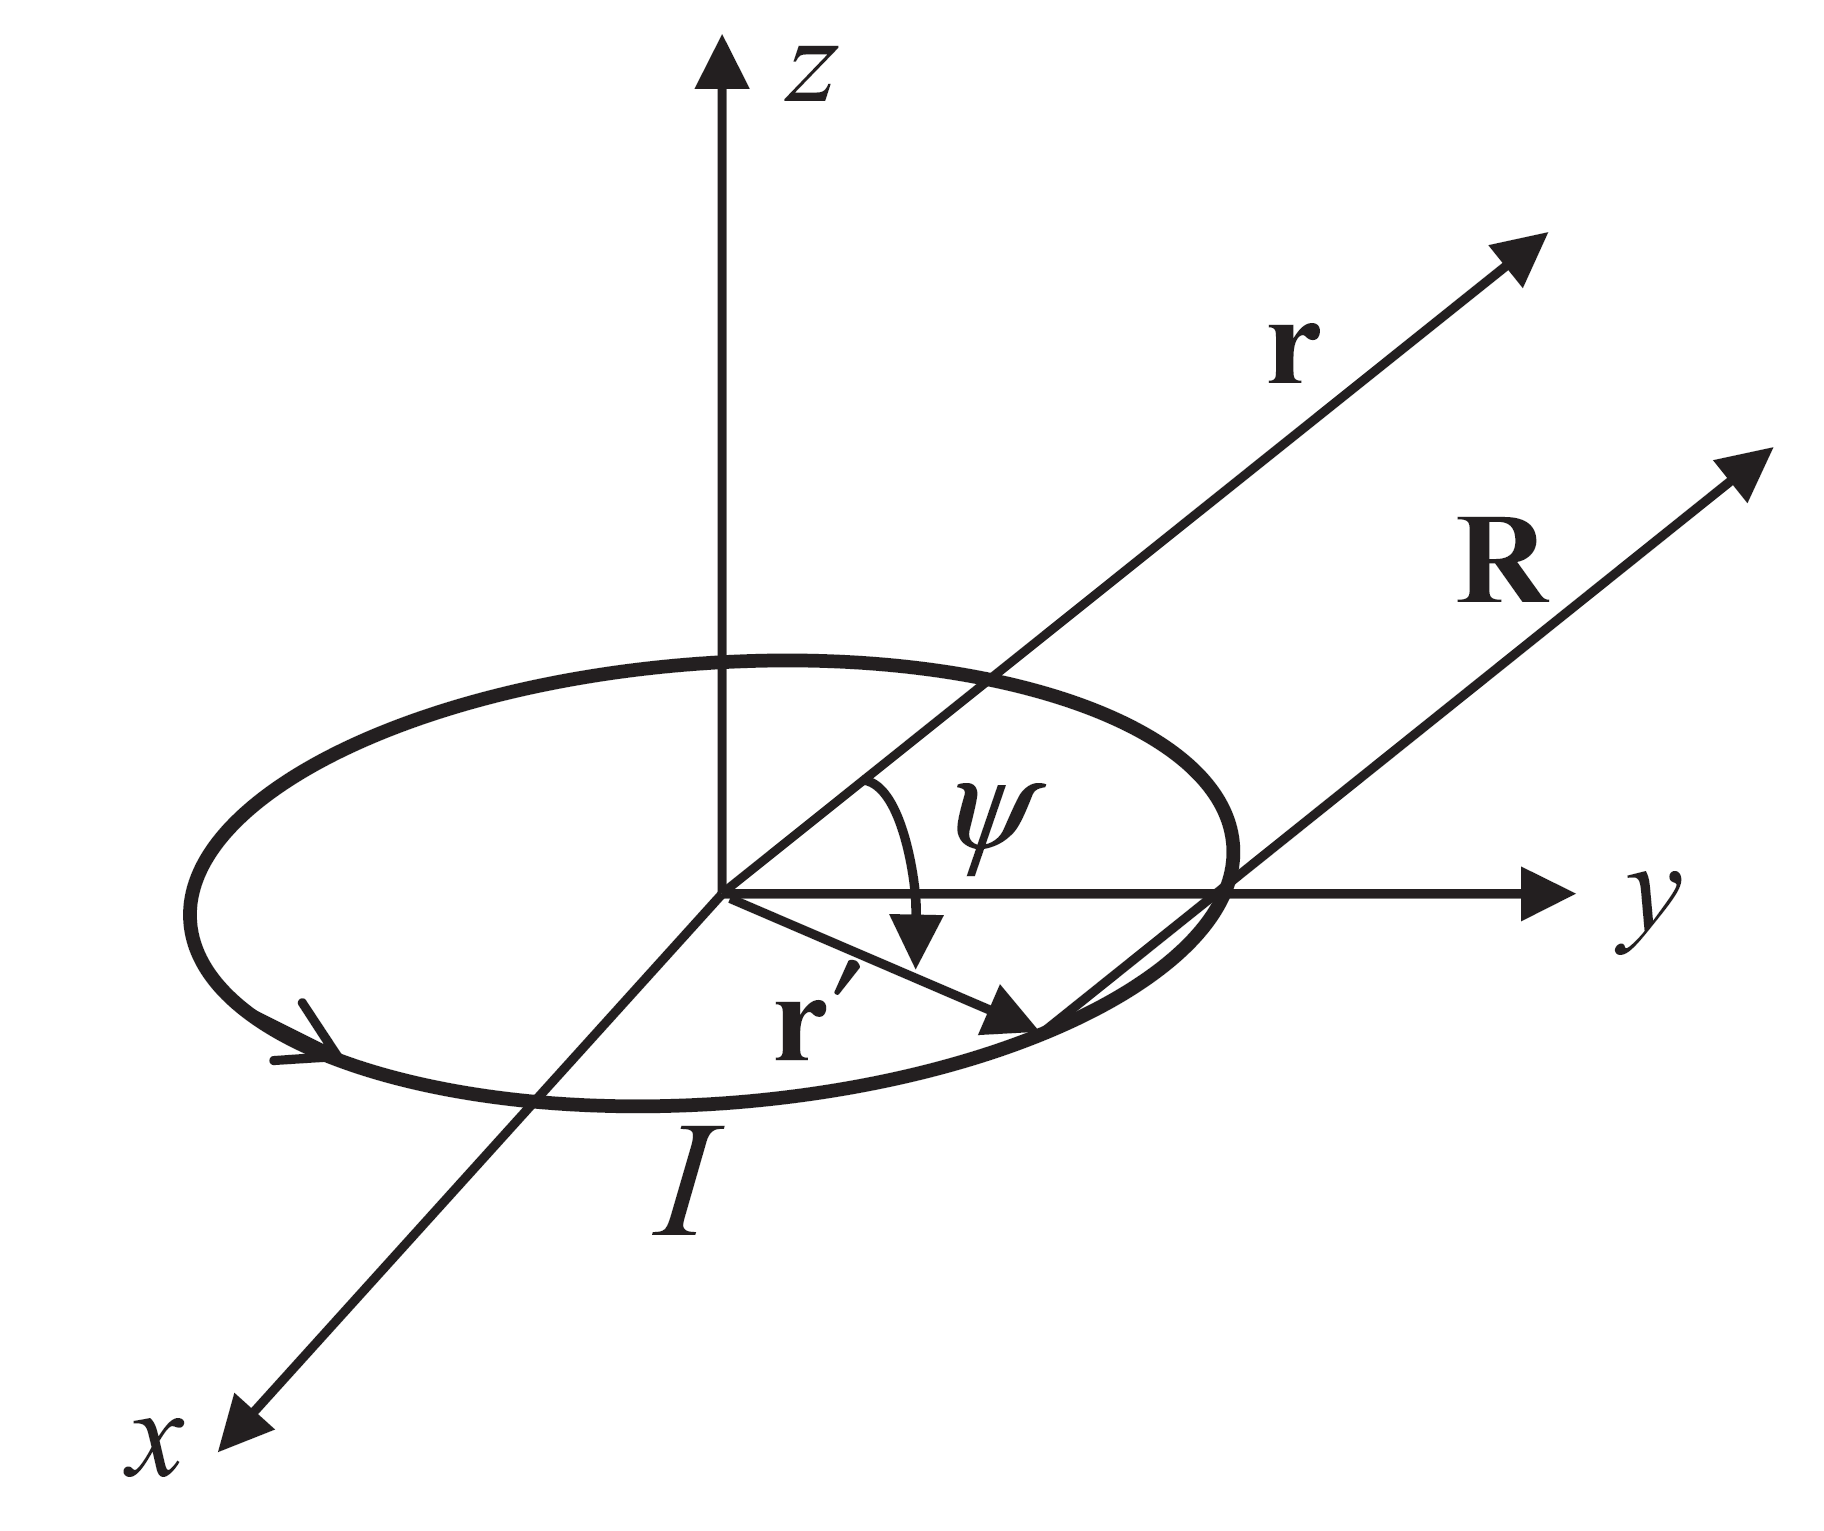
\includegraphics[width=0.3\textwidth]{圆电流环.PNG}
    \caption{圆电流环}
    \label{fig:fig3}
\end{figure}
考虑一个半径为$a$,携带均匀时谐电流$\mathbf{I}=\hat{\phi}I$的圆环,如图\ref{fig:fig3}所示。则在远场区,
\begin{align}
    \label{eq:eq135}
    E_{\phi}&\approx\frac{\eta(ka)^2I}{4r}e^{-jkr}\sin\theta \\
    \label{eq:eq136}
    H_{\theta}&\approx-\frac{(ka)^2I}{4r}e^{-jkr}\sin\theta
\end{align}
考虑一个长度为$l$,磁流为$K$的$z$方向无限小磁偶极子,在远场区,
\begin{align}
    \label{eq:eq156}
    E_{\phi}&\approx-\frac{jkKl}{4\pi r}e^{-jkr}\sin\theta \\
    \label{eq:eq157}
    H_{\theta}&\approx\frac{jkKl}{4\eta\pi r}e^{-jkr}\sin\theta
\end{align}
对比可得,小电流环与小磁偶极子是等效的,其中磁偶极子的磁矩为$Kl=jw\mu IS$,$S=\pi a^2$是磁流环的面积。无限小电流环与磁偶极子不仅远场相同,近场也相同。
\subsubsection{面电流}
\begin{figure}[ht]
    \centering
    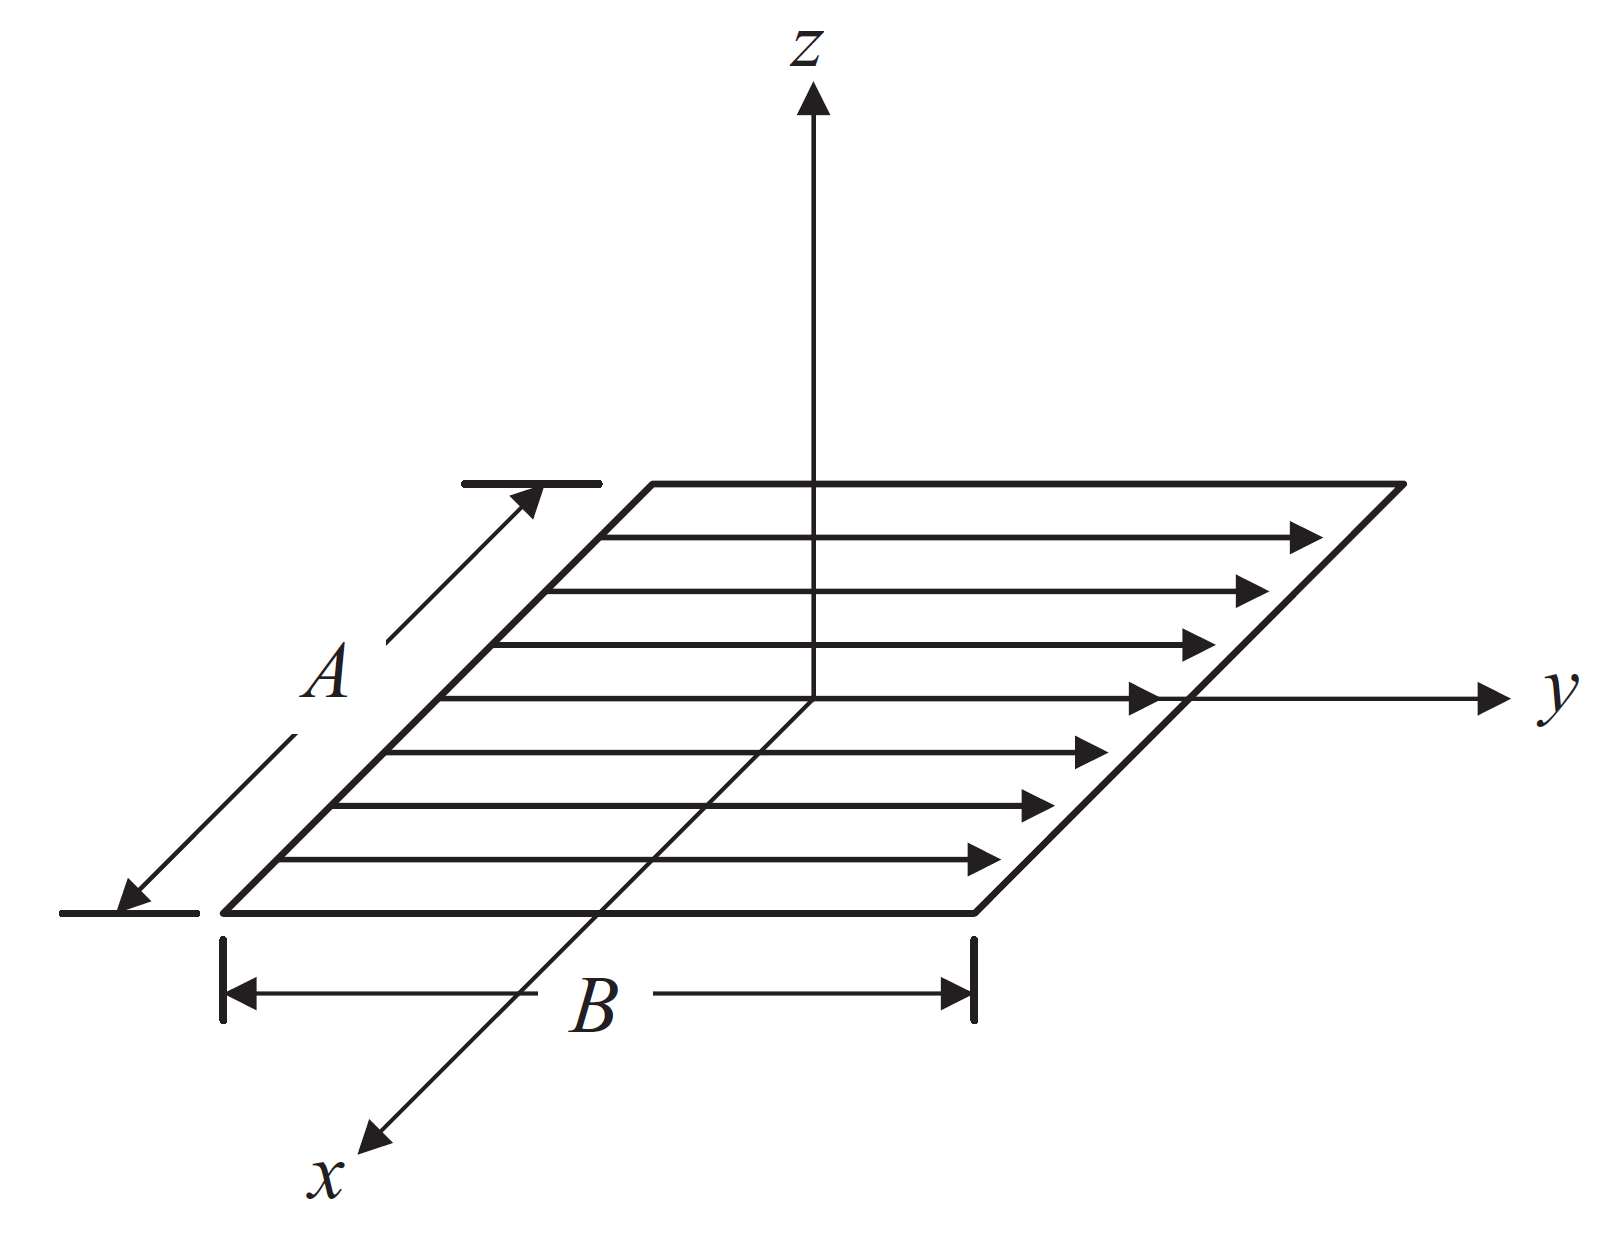
\includegraphics[width=0.35\textwidth]{面电流.PNG}
    \caption{面电流}
    \label{fig:fig4}
\end{figure}
考虑一个位于$xy$平面上,长为$A$,宽为$B$的矩形面电流,如图\ref{fig:fig4}所示。其电流密度为
\begin{align}
    \label{eq:eq139}
    \mathbf{J}_S(x,y)=\hat{y}J_0e^{-j(h_xx+h_yy)}
\end{align}
式中,$J_0$、$h_x$、$h_y$为常数。则电场远场为:
\begin{align}
    \label{eq:eq137}
    E_{\theta}&\approx-\frac{jk\eta J_0AB}{4\pi r}e^{-jkr}\cos\theta\sin\phi\frac{\sin X}{X}\frac{\sin Y}{Y} \\
    \label{eq:eq138}
    H_{\phi}&\approx\frac{jk\eta J_0AB}{4\pi r}e^{-jkr}\cos\phi\frac{\sin X}{X}\frac{\sin Y}{Y}
\end{align}
式中,
\begin{align}
    \label{eq:eq140}
    X=(k\sin\theta\cos\phi-h_x)\frac{A}{2} \\
    \label{eq:eq141}
    Y=(k\sin\theta\sin\phi-h_y)\frac{B}{2}
\end{align}
若用两个参量$\theta_{S}$、$\phi_{S}$来控制相位常数,即
\begin{align}
    \label{eq:eq142}
    h_x=k\sin\theta_{S}\cos\phi_{S} \\
    \label{eq:eq143}
    h_y=k\sin\theta_{S}\sin\phi_{S}
\end{align}
则
\begin{align}
    \label{eq:eq144}
    X=(\sin\theta\cos\phi-\sin\theta_{S}\cos\phi_{S})\frac{kA}{2} \\
    \label{eq:eq145}
    Y=(\sin\theta\sin\phi-\sin\theta_{S}\sin\phi_{S})\frac{kB}{2}
\end{align}
可以看出,辐射场在$\theta=\theta_S$、$\phi=\phi_S$和$\theta=\pi-\theta_S$、$\phi=\phi_S$两个方向上幅度最大,因此可以通过调整参数$\theta_{S}$、$\phi_{S}$来控制辐射场的最大方向。
此外,$A$越大,$\phi=0$面的波束宽度越小,$B$越大,$\phi=\pi/2$面的波束宽度越小,即,面电流面积越大,波束宽度越窄。
\par
对于任意的面电流,$J_x$和$J_y$往往同时存在,总的辐射场是由$J_x$和$J_y$产生的场的叠加。
\subsubsection{平面阵}
\begin{figure}[ht]
    \centering
    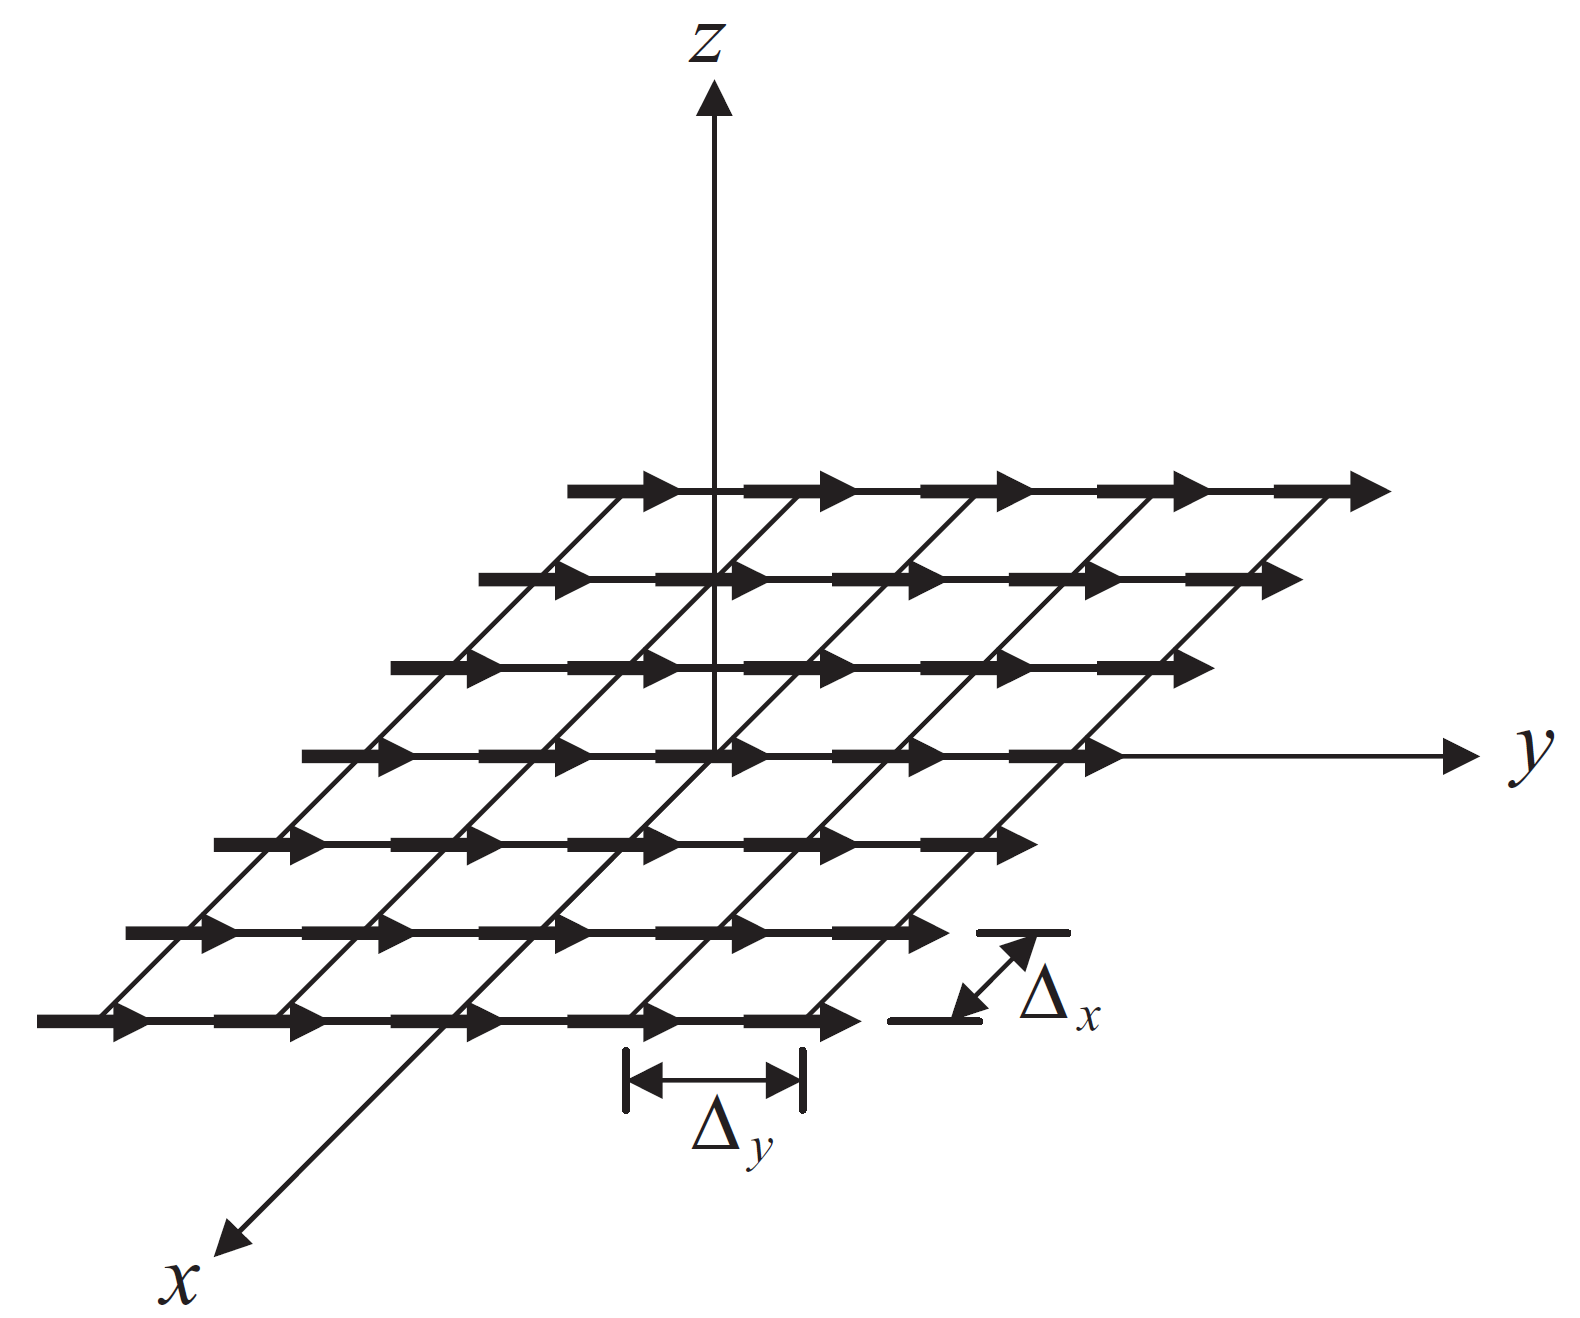
\includegraphics[width=0.35\textwidth]{平面阵.PNG}
    \caption{平面阵}
    \label{fig:fig5}
\end{figure}
考虑一个位于$xy$平面的$y$方向偶极子阵,每个偶极子的幅度和相位可以独立控制(相控阵),如图\ref{fig:fig5}所示。假设阵元是偶极矩为$Il$的无限小电偶极子,偶极子的位置为$(x_i,y_i)$,相位为$\varphi_i$,$i=1,2,\cdots,N$,$N$为偶极子的总数。偶极子阵的总辐射场是阵元辐射场的叠加,则在远场,
\begin{align}
    \label{eq:eq146}
    E_{\theta}&\approx-\frac{jk\eta Il}{4\pi r}e^{-jkr}\cos\theta\sin\phi\sum_{i=1}^{N}e^{j[k(x_i\sin\theta\cos\phi+y_i\sin\theta\sin\phi)+\varphi_i]} \\
    \label{eq:eq147}
    E_{\phi}&\approx-\frac{jk\eta Il}{4\pi r}e^{-jkr}\cos\phi\sum_{i=1}^{N}e^{j[k(x_i\sin\theta\cos\phi+y_i\sin\theta\sin\phi)+\varphi_i]}
\end{align}
定义阵因子:
\begin{align}
    \label{eq:eq148}
    AF(\theta,\phi)=\sum_{i=1}^{N}e^{j[k(x_i\sin\theta\cos\phi+y_i\sin\theta\sin\phi)+\varphi_i]}
\end{align}
阵元辐射方向图:
\begin{align}
    \label{eq:eq149}
    e_{\theta}(\theta,\phi)=Il\cos\theta\sin\phi \\
    \label{eq:eq150}
    e_{\phi}(\theta,\phi)=Il\cos\phi
\end{align}
则阵列的总辐射远场表示为:
\begin{align}
    \label{eq:eq151}
    \mathbf{E}\approx-\frac{jk\eta}{4\pi r}e^{-jkr}\vec{e}(\theta,\phi)AF(\theta,\phi)
\end{align}
若每个偶极子的幅度独立控制,则
\begin{align}
    \label{eq:eq152}
    AF(\theta,\phi)=\sum_{i=1}^{N}\frac{I_i}{I_0}e^{j[k(x_i\sin\theta\cos\phi+y_i\sin\theta\sin\phi)+\varphi_i]}
\end{align}
式中,$I_i$为第$i$个偶极子的幅度,$I_0$是产生阵元方向图为$\vec{e}(\theta,\phi)$的偶极子的幅度。
\par
考虑一个矩形偶极子阵,$x$、$y$方向上的偶极子数目分别为$N_x+1$、$N_y+1$($N_x$、$N_y$均为偶数),相邻偶极子的间距分别为$\Delta_x$、$\Delta_y$,则第$i$个偶极子的位置为$x_i=i_x\Delta_x$,$y_i=i_y\Delta_y$,$i_x=-N_x/2,\cdots,N_x/2$,$i_y=-N_y/2,\cdots,N_y/2$,第$i$个偶极子的相位为$\phi_i=-h_xi_x\Delta_x-h_yi_y\Delta_y$,则
\begin{align}
    \label{eq:eq153}
    AF(\theta,\phi)&=\sum_{i_x=-N_x/2}^{N_x/2}e^{j(k\sin\theta\cos\phi-h_x)i_x\Delta_x}\sum_{i_y=-N_y/2}^{N_y/2}e^{j(k\sin\theta\cos\phi-h_y)i_y\Delta_y} \nonumber \\
                   &=\frac{\sin\left(\frac{N_x+1}{2}\psi_x\right)}{\sin\frac{\psi_x}{2}}\frac{\sin\left(\frac{N_y+1}{2}\psi_y\right)}{\sin\frac{\psi_y}{2}}
\end{align}
式中,
\begin{align}
    \label{eq:eq154}
    \psi_x=(k\sin\theta\cos\phi-h_x)\Delta_x \\
    \label{eq:eq155}
    \psi_y=(k\sin\theta\cos\phi-h_y)\Delta_y
\end{align}
若用两个参量$\theta_{S}$、$\phi_{S}$来控制相位常数$h_x$、$h_y$,如式\ref{eq:eq142}、式\ref{eq:eq143}所示,则有
\begin{align}
    \label{eq:eq158}
    \psi_x=(\sin\theta\cos\phi-\sin\theta_{S}\cos\phi_{S})k\Delta_x \\
    \label{eq:eq159}
    \psi_y=(\sin\theta\cos\phi-\sin\theta_{S}\sin\phi_{S})k\Delta_y
\end{align}
最大辐射方向为$\psi_x=2m\pi$和$\psi_y=2n\pi$,$m,n=0,1,2,\cdots$,对应$m=n=0$的辐射方向为$(\theta_S,\phi_S)$和$(\pi-\theta_S,\phi_S)$。为了确保天线阵只有两个最大的方向,需满足$\Delta_x<\lambda$和$\Delta_y<\lambda$。
\section{\textsf{电磁定理和原理}}
\subsection{唯一性定理}
\begin{figure}[ht]
    \centering
    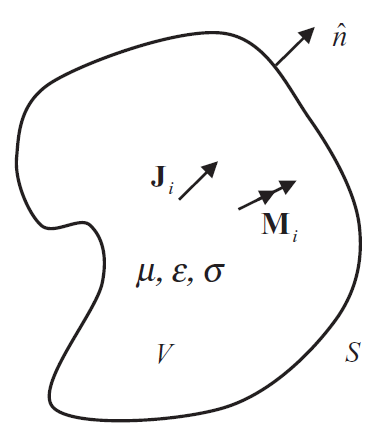
\includegraphics[width=0.25\textwidth]{唯一性定理.PNG}
    \caption{空间$V$内的电流源和磁流源}
    \label{fig:fig6}
\end{figure}
考虑由面$S$包围的体积$V$,体积内的介质的介电常数为$\epsilon$,磁导率为$\mu$,电导率为$\sigma$,体积内包含电流源和磁流源,电流密度为$\mathbf{J}_i$,磁流密度为$\mathbf{M}_i$,如图\ref{fig:fig6}所示。假设源产生两组不同的场,分别为$(\mathbf{E}^a,\mathbf{H}^a)$和$(\mathbf{E}^b,\mathbf{H}^b)$。则有
\begin{align}
    \label{eq:eq160}
    \nabla \times \mathbf{E}^a&=-jw\mu\mathbf{H}^a-\mathbf{M}_i &\nabla \times \mathbf{H}^a=jw\epsilon\mathbf{E}^a+\sigma\mathbf{E}^a+\mathbf{J}_i \\
    \label{eq:eq162}
    \nabla \times \mathbf{E}^b&=-jw\mu\mathbf{H}^b-\mathbf{M}_i &\nabla \times \mathbf{H}^b=jw\epsilon\mathbf{E}^b+\sigma\mathbf{E}^b+\mathbf{J}_i
\end{align}
两式相减,得
\begin{align}
    \label{eq:eq161}
    \nabla \times \delta \mathbf{E}&=-jw\mu\delta\mathbf{H} \\
    \label{eq:eq163}
    \nabla \times \delta \mathbf{H}&=jw\mu\delta\mathbf{E}+\sigma\delta\mathbf{E}
\end{align}
式中,$\delta \mathbf{E}=\mathbf{E}^a-\mathbf{E}^b$,$\delta \mathbf{H}=\mathbf{H}^a-\mathbf{H}^b$,则
\begin{align}
    \label{eq:eq164}
    \delta\mathbf{H}^*\cdot\nabla\times\delta\mathbf{E}-\delta\mathbf{E}\cdot\nabla\times\delta\mathbf{H}^*&=\nabla\cdot(\delta\mathbf{E}\times\delta\mathbf{H}^*) \nonumber \\
            &=-jw\mu\left|\delta\mathbf{H}\right|^2+(jw\epsilon^*-\sigma)\left|\delta\mathbf{E}\right|^2
\end{align}
对上式进行体积分,并利用高斯定理,有
\begin{align}
    \label{eq:eq165}
    \iiint_V \nabla\cdot(\delta\mathbf{E}\times\delta\mathbf{H}^*)dV&=\varoiint_S (\delta\mathbf{E}\times\delta\mathbf{H}^*)\cdot d\mathbf{S} \nonumber \\
        &=\iiint_V \left[-jw\mu\left|\delta\mathbf{H}\right|^2+(jw\epsilon^*-\sigma)\left|\delta\mathbf{E}\right|^2\right]dV
\end{align}
如果\\
(1)在整个$S$面,切向电场$(\hat{n}\times\mathbf{E})$是给定的,从而在$S$面上$\hat{n}\times\delta\mathbf{E}=0$;\\
(2)在整个$S$面,切向磁场$(\hat{n}\times\mathbf{H})$是给定的,从而在$S$面上$\hat{n}\times\delta\mathbf{H}=0$;\\
(3)在$S$面的一部分,切向电场$(\hat{n}\times\mathbf{E})$是给定的,其余部分,切向磁场$(\hat{n}\times\mathbf{H})$是给定的。\\
三个条件满足其中之一,则上式得面积分为零,即
\begin{align}
    \label{eq:eq166}
    \iiint_V \left[-jw\mu\left|\delta\mathbf{H}\right|^2+(jw\epsilon^*-\sigma)\left|\delta\mathbf{E}\right|^2\right]dV=0
\end{align}
对于一般的损耗媒质,$\mu=\mu'-j\mu''(\mu''\geq 0)$,$\epsilon=\epsilon'-j\epsilon''(\epsilon''\geq 0)$,式\ref{eq:eq166}的实部为
\begin{align}
    \label{eq:eq167}
    \iiint_V \left[w\mu''\left|\delta\mathbf{H}\right|^2+(w\epsilon''+\sigma)\left|\delta\mathbf{E}\right|^2\right]dV=0
\end{align}
虚部为
\begin{align}
    \label{eq:eq168}
    \iiint_V \left[-w\mu'\left|\delta\mathbf{H}\right|^2+w\epsilon'\left|\delta\mathbf{E}\right|^2\right]dV=0
\end{align}
因此,不论是什么类型的损耗,只要媒质是有耗的,且$w>0$,就有$\delta\mathbf{E}=0$和$\delta\mathbf{H}=0$。也可以将无耗媒质和静态场情况当成有耗和频率无限接近于零的情况,则上述结论对无耗媒质和静态场情况也适用。
\par
\textbf{\color{blue}{唯一性定理}}:当一个空间内的源给定,且其表面上的切向电场分量或切向磁场分量给定,或者表面的一部分切向电场分量给定,其余部分切向磁场分量给定,这时在该空间内的场是唯一确定的。
\subsection{镜像原理}
\subsubsection{基本思想}
对于非自由空间求解辐射场问题,需要联立麦克斯韦方程组以及边界条件进行求解,过程相当复杂。但可以将非自由空间问题转换成一个等效的自由空间问题,然后利用自由空间的场-源关系得到它的解。
\par
现构建一个新问题,在非自由空间以外的空间添加媒质以及新的源,等效为一个自由空间,使得原问题中的非自由空间的边界条件在新问题中也同样满足。那么,在新问题中的原非自由空间内的源于原问题一致,边界条件一致,根据唯一性定理,原非自由空间内的场与新问题在相同空间内的场相同。
\par
图\ref{fig:fig7}给出了位于无限大导电体(PEC)平面上方的水平电偶极子、垂直电偶极子、水平磁偶极子、垂直磁偶极子在平面下方的镜像源;图\ref{fig:fig8}给出了无限大平面是导磁体(PMC)的情况。
\begin{figure}[ht]
    \centering
    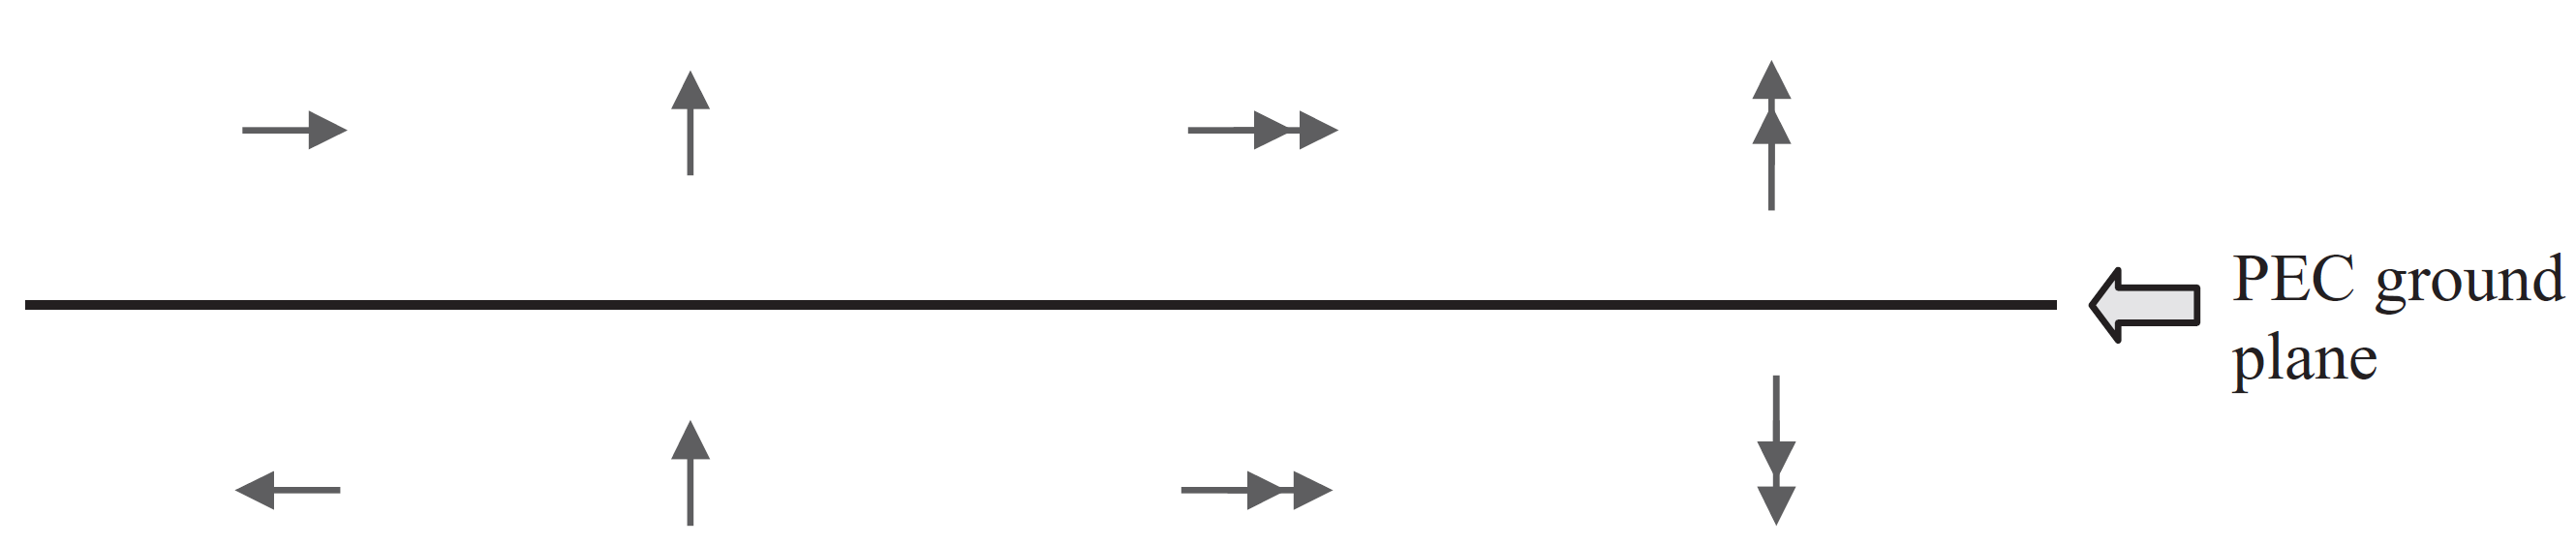
\includegraphics[width=0.8\textwidth]{PEC平面上方的电偶极子和磁偶极子的镜像.PNG}
    \caption{PEC平面上方的电偶极子和磁偶极子的镜像}
    \label{fig:fig7}
\end{figure}
\begin{figure}[ht]
    \centering
    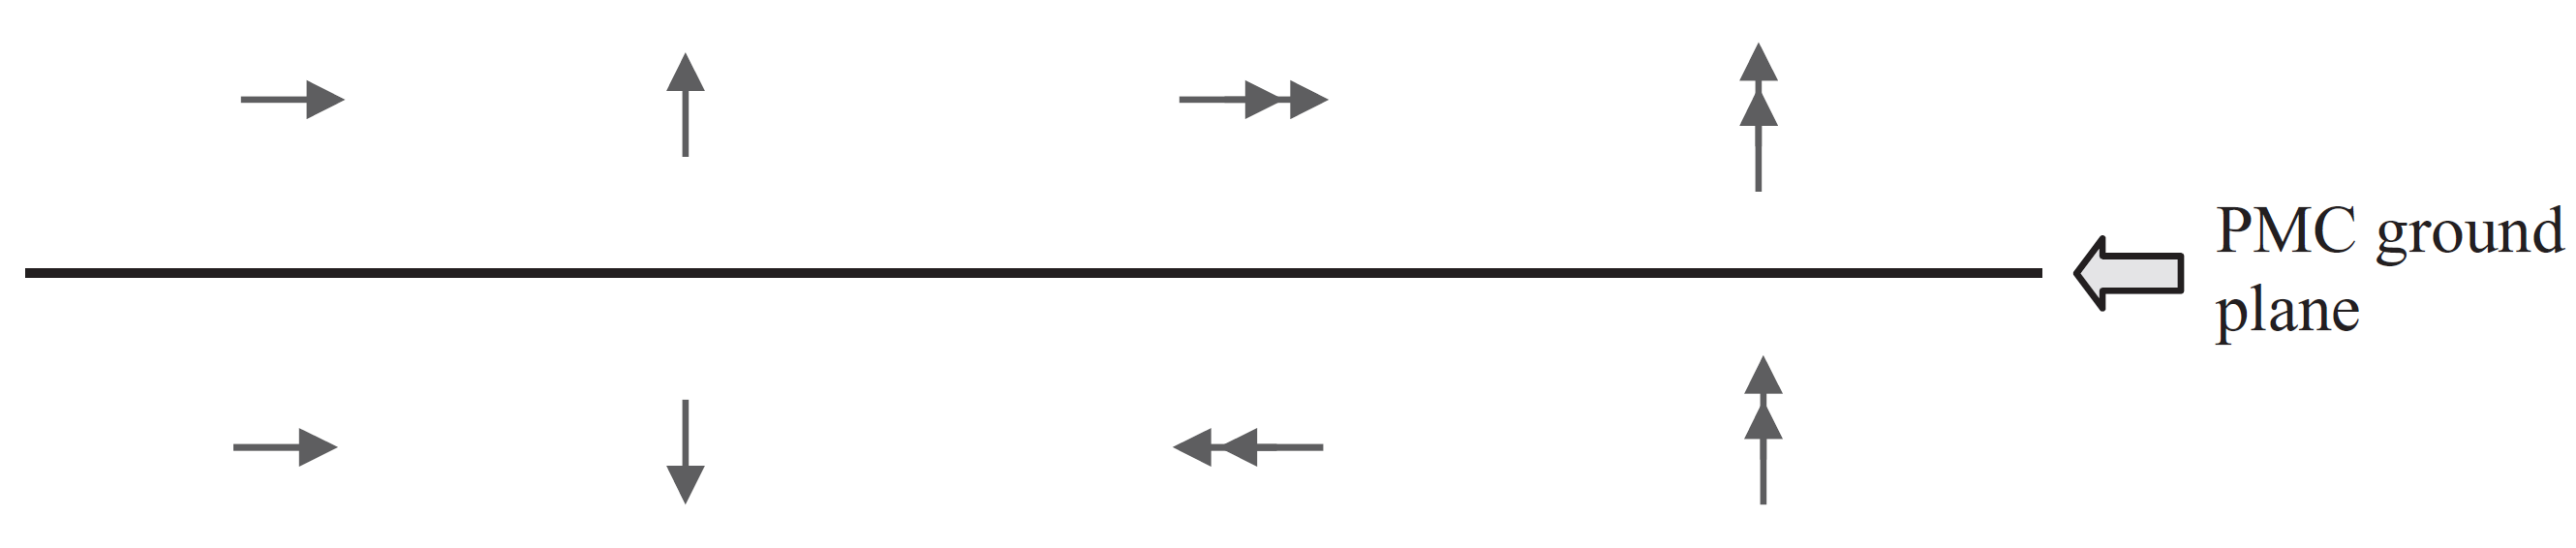
\includegraphics[width=0.8\textwidth]{PMC平面上方的电偶极子和磁偶极子的镜像.PNG}
    \caption{PMC平面上方的电偶极子和磁偶极子的镜像}
    \label{fig:fig8}
\end{figure}
\par
对于任意电(磁)流源,可以分解成无数个很小的垂直和水平电(磁)偶极子,因此,图\ref{fig:fig7}和图\ref{fig:fig8}给出的镜像原理可以应用于任意电(磁)流源。
根据图\ref{fig:fig7}和图\ref{fig:fig8},令平面的位置为$z=0$,$\vec{r}_i=\hat{x}x+\hat{y}y-\hat{z}z$是$\vec{r}=\hat{x}x+\hat{y}y+\hat{z}z$的镜像位置。\\
(1)考虑一个无限大PEC平面上方的电流密度为$\mathbf{J}(\vec{r})$的电流源:
\begin{align}
    \label{eq:eq169}
    \mathbf{J}(\vec{r})=\mathbf{J}_v(\vec{r})+\mathbf{J}_h(\vec{r})=\hat{z}\hat{z}\cdot\mathbf{J}(\vec{r})+[\mathbf{J}(\vec{r})-\hat{z}\hat{z}\cdot\mathbf{J}(\vec{r})]
\end{align}
则其镜像源为:
\begin{align}
    \label{eq:eq170}
    \mathbf{J}^{im}(\vec{r})&=\mathbf{J}^{im}_v(\vec{r})+\mathbf{J}^{im}_h(\vec{r})=\mathbf{J}_v(\vec{r}_i)-\mathbf{J}_h(\vec{r}_i) \nonumber \\
                            &=\hat{z}\hat{z}\cdot\mathbf{J}(\vec{r}_i)-[\mathbf{J}(\vec{r}_i)-\hat{z}\hat{z}\cdot\mathbf{J}(\vec{r}_i)]=2\hat{z}\hat{z}\cdot\mathbf{J}(\vec{r}_i)-\mathbf{J}(\vec{r}_i)
\end{align}
(2)考虑一个无限大PEC平面上方的磁流密度为$\mathbf{M}(\vec{r})$的磁流源:
\begin{align}
    \label{eq:eq171}
    \mathbf{M}(\vec{r})=\mathbf{M}_v(\vec{r})+\mathbf{M}_h(\vec{r})=\hat{z}\hat{z}\cdot\mathbf{M}(\vec{r})+[\mathbf{M}(\vec{r})-\hat{z}\hat{z}\cdot\mathbf{M}(\vec{r})]
\end{align}
则其镜像源为:
\begin{align}
    \label{eq:eq172}
    \mathbf{M}^{im}(\vec{r})&=\mathbf{M}^{im}_v(\vec{r})+\mathbf{M}^{im}_h(\vec{r})=-\mathbf{M}_v(\vec{r}_i)+\mathbf{M}_h(\vec{r}_i) \nonumber \\
                            &=-\hat{z}\hat{z}\cdot\mathbf{M}(\vec{r}_i)+[\mathbf{M}(\vec{r}_i)-\hat{z}\hat{z}\cdot\mathbf{M}(\vec{r}_i)]=-2\hat{z}\hat{z}\cdot\mathbf{M}(\vec{r}_i)+\mathbf{M}(\vec{r}_i)
\end{align}
(3)考虑一个无限大PMC平面上方的电流密度为$\mathbf{J}(\vec{r})$的电流源:
\begin{align}
    \label{eq:eq173}
    \mathbf{J}(\vec{r})=\mathbf{J}_v(\vec{r})+\mathbf{J}_h(\vec{r})=\hat{z}\hat{z}\cdot\mathbf{J}(\vec{r})+[\mathbf{J}(\vec{r})-\hat{z}\hat{z}\cdot\mathbf{J}(\vec{r})]
\end{align}
则其镜像源为:
\begin{align}
    \label{eq:eq174}
    \mathbf{J}^{im}(\vec{r})&=\mathbf{J}^{im}_v(\vec{r})+\mathbf{J}^{im}_h(\vec{r})=-\mathbf{J}_v(\vec{r}_i)+\mathbf{J}_h(\vec{r}_i) \nonumber \\
                            &=-\hat{z}\hat{z}\cdot\mathbf{J}(\vec{r}_i)+[\mathbf{J}(\vec{r}_i)-\hat{z}\hat{z}\cdot\mathbf{J}(\vec{r}_i)]=-2\hat{z}\hat{z}\cdot\mathbf{J}(\vec{r}_i)+\mathbf{J}(\vec{r}_i)
\end{align}
(4)考虑一个无限大PMC平面上方的磁流密度为$\mathbf{M}(\vec{r})$的磁流源:
\begin{align}
    \label{eq:eq175}
    \mathbf{M}(\vec{r})=\mathbf{M}_v(\vec{r})+\mathbf{M}_h(\vec{r})=\hat{z}\hat{z}\cdot\mathbf{M}(\vec{r})+[\mathbf{M}(\vec{r})-\hat{z}\hat{z}\cdot\mathbf{M}(\vec{r})]
\end{align}
则其镜像源为:
\begin{align}
    \label{eq:eq176}
    \mathbf{M}^{im}(\vec{r})&=\mathbf{M}^{im}_v(\vec{r})+\mathbf{M}^{im}_h(\vec{r})=\mathbf{M}_v(\vec{r}_i)-\mathbf{M}_h(\vec{r}_i) \nonumber \\
                            &=\hat{z}\hat{z}\cdot\mathbf{M}(\vec{r}_i)-[\mathbf{M}(\vec{r}_i)-\hat{z}\hat{z}\cdot\mathbf{M}(\vec{r}_i)]=2\hat{z}\hat{z}\cdot\mathbf{M}(\vec{r}_i)-\mathbf{M}(\vec{r}_i)
\end{align}
\par
考虑其他非自由空间,对于一个垂直无限大PEC平面和一个水平无限大PEC平面相交形成的直角劈区域,一个垂直电流源的镜像源如图\ref{fig:fig9}所示。
\begin{figure}[ht]
    \centering
    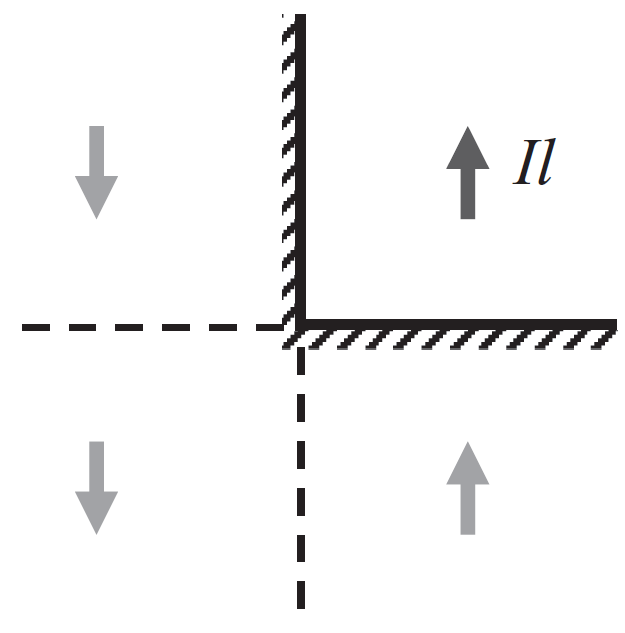
\includegraphics[width=0.2\textwidth]{置于直角PEC劈中的垂直电流源.PNG}
    \caption{置于直角PEC劈中的垂直电流源}
    \label{fig:fig9}
\end{figure}
\par
对于$60^\circ $角PEC斜劈区域,一个平行线电流源的镜像源如图\ref{fig:fig10}所示。
\begin{figure}[ht]
    \centering
    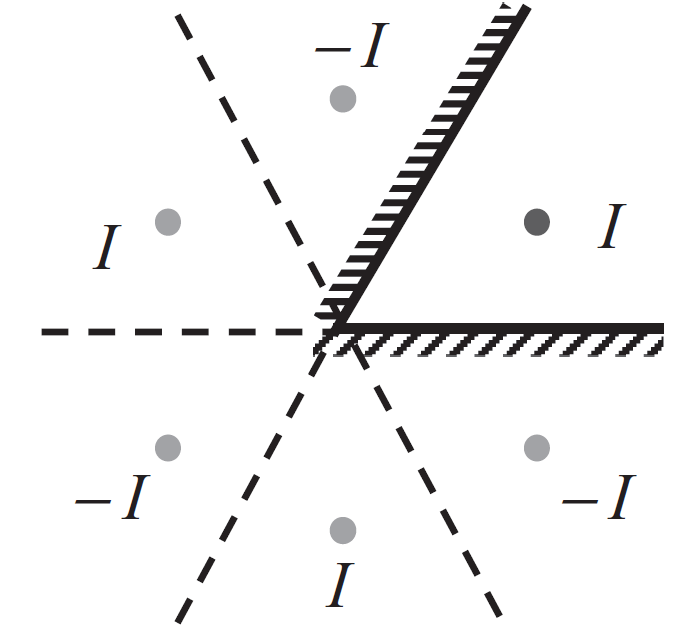
\includegraphics[width=0.2\textwidth]{置于60角PEC斜劈中的平行线电流源.PNG}
    \caption{置于$60^\circ $角PEC斜劈中的平行线电流源}
    \label{fig:fig10}
\end{figure}
\par
对于其他非特殊角度,可能需要无数个镜像源才能保证总场满足边界条件,且由于这些镜像源位于场区附近,总场的求和式不收敛,得不到一个最终的解析公式。
一个特殊的例子:位于两个平行放置的无限大PEC平面之间区域的倾斜电流源同样具有无数个镜像源,如图\ref{fig:fig11}所示。但由于镜像源与场区越来越远,因此总场的求和式收敛,可以得到解析解。
\begin{figure}[ht]
    \centering
    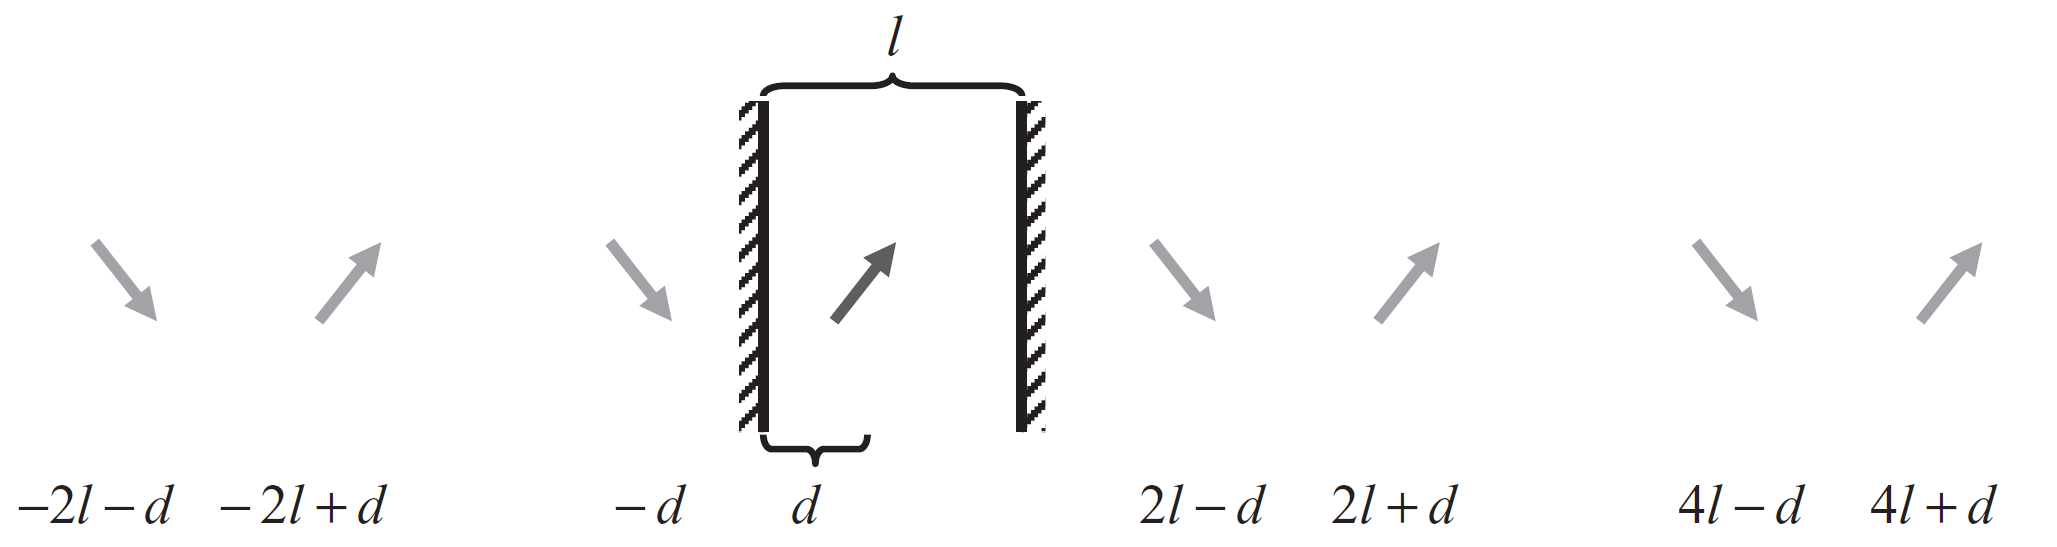
\includegraphics[width=0.5\textwidth]{置于两个无限大PEC平面之间的倾斜电流源.PNG}
    \caption{置于两个无限大PEC平面之间的倾斜电流源}
    \label{fig:fig11}
\end{figure}
\par
镜像原理可以用于源在矩形波导和矩形谐振腔中的辐射问题,还可以应用到一些特殊的导体曲面、平面介质半空间及分层媒质问题中。对于这些问题,镜像源与原来的源形状一般是不同的。
\subsubsection{无限大半空间中的场-源关系}
考虑无限大PEC平面,位于$z=0$,上半空间有电流源$\mathbf{J}(\vec{r})$和磁流源$\mathbf{M}(\vec{r})$,根据式\ref{eq:eq170}和式\ref{eq:eq172},镜像源为
\begin{align}
    \label{eq:eq177}
    \mathbf{J}^{im}(\vec{r})&=2\hat{z}\hat{z}\cdot\mathbf{J}(\vec{r}_i)-\mathbf{J}(\vec{r}_i) \\
    \label{eq:eq178}
    \mathbf{M}^{im}(\vec{r})&=-2\hat{z}\hat{z}\cdot\mathbf{M}(\vec{r}_i)+\mathbf{M}(\vec{r}_i)
\end{align}
根据式\ref{eq:eq110}得,电场表达式为:
\begin{align}
    \label{eq:eq179}
    \mathbf{E}(\vec{r})&=-jw\mu\iiint_V\overline{\mathbf{G}}_{e0}(\vec{r},\vec{r}')\cdot \mathbf{J}(\vec{r}')dV'-\iiint_V\overline{\mathbf{G}}_{m0}(\vec{r},\vec{r}')\cdot \mathbf{M}(\vec{r}')dV' \nonumber \\
                       &\qquad-jw\mu\iiint_{V_{im}}\overline{\mathbf{G}}_{e0}(\vec{r},\vec{r}')\cdot \mathbf{J}^{im}(\vec{r}')dV'-\iiint_{V_{im}}\overline{\mathbf{G}}_{m0}(\vec{r},\vec{r}')\cdot \mathbf{M}^{im}(\vec{r}')dV' \nonumber \\
                       &=-jw\mu\iiint_V\overline{\mathbf{G}}_{e0}(\vec{r},\vec{r}')\cdot \mathbf{J}(\vec{r}')dV'-\iiint_V\overline{\mathbf{G}}_{m0}(\vec{r},\vec{r}')\cdot \mathbf{M}(\vec{r}')dV' \nonumber \\
                       &\qquad-jw\mu\iiint_{V_{im}}\overline{\mathbf{G}}_{e0}(\vec{r},\vec{r}')\cdot [2\hat{z}\hat{z}\cdot\mathbf{J}(\vec{r}'_i)-\mathbf{J}(\vec{r}'_i)]dV' \nonumber \\
                       &\qquad+\iiint_{V_{im}}\overline{\mathbf{G}}_{m0}(\vec{r},\vec{r}')\cdot [2\hat{z}\hat{z}\cdot\mathbf{M}(\vec{r}'_i)-\mathbf{M}(\vec{r}'_i)]dV' \nonumber \\
                       &\xlongequal{V_{im}\to V}-jw\mu\iiint_V\left[\overline{\mathbf{G}}_{e0}(\vec{r},\vec{r}')-\overline{\mathbf{G}}_{e0}(\vec{r},\vec{r}'_i)+2\overline{\mathbf{G}}_{e0}(\vec{r},\vec{r}'_i)\cdot\hat{z}\hat{z}\right]\cdot\mathbf{J}(\vec{r}')dV' \nonumber \\
                       &\qquad-\iiint_V\left[\overline{\mathbf{G}}_{m0}(\vec{r},\vec{r}')+\overline{\mathbf{G}}_{m0}(\vec{r},\vec{r}'_i)-2\overline{\mathbf{G}}_{m0}(\vec{r},\vec{r}'_i)\cdot\hat{z}\hat{z}\right]\cdot\mathbf{M}(\vec{r}')dV' \nonumber \\
                       &=-jw\mu\iiint_V\overline{\mathbf{G}}_{e1}(\vec{r},\vec{r}')dV'-\iiint_V\overline{\mathbf{G}}_{m1}(\vec{r},\vec{r}')dV'
\end{align}
式中,
\begin{align}
    \label{eq:eq180}
    \overline{\mathbf{G}}_{e1}(\vec{r},\vec{r}')&=\overline{\mathbf{G}}_{e0}(\vec{r},\vec{r}')-\overline{\mathbf{G}}_{e0}(\vec{r},\vec{r}'_i)+2\overline{\mathbf{G}}_{e0}(\vec{r},\vec{r}'_i)\cdot\hat{z}\hat{z} \\
    \label{eq:eq181}
    \overline{\mathbf{G}}_{m1}(\vec{r},\vec{r}')&=\overline{\mathbf{G}}_{m0}(\vec{r},\vec{r}')+\overline{\mathbf{G}}_{m0}(\vec{r},\vec{r}'_i)-2\overline{\mathbf{G}}_{m0}(\vec{r},\vec{r}'_i)\cdot\hat{z}\hat{z}
\end{align}
称$\overline{\mathbf{G}}_{e1}$为\textbf{\color{blue}{第一类半空间电并矢格林函数}},$\overline{\mathbf{G}}_{m1}$为\textbf{\color{blue}{第一类半空间磁并矢格林函数}}。在$z=0$处满足第一类边界条件:
\begin{align}
    \label{eq:eq182}
    \hat{z}\times\overline{\mathbf{G}}_{e1}(\vec{r},\vec{r}')=\hat{z}\times\overline{\mathbf{G}}_{m1}(\vec{r},\vec{r}')=0
\end{align}
将式\ref{eq:eq108}、式\ref{eq:eq109}代入式\ref{eq:eq180}、式\ref{eq:eq181},并利用相关代数关系\footnote{$\nabla f(\vec{r}-\vec{r}')=-\nabla'f(\vec{r}-\vec{r}')\qquad\nabla f(\vec{r}-\vec{r}'_i)=-\nabla'f(\vec{r}-\vec{r}'_i)+2\hat{z}\hat{z}\cdot\nabla f(\vec{r}-\vec{r}'_i)$\label{fn:fn0}},得
\begin{align}
    \label{eq:eq183}
    \overline{\mathbf{G}}_{e1}(\vec{r},\vec{r}')&=\left(\overline{\mathbf{I}}-\frac{1}{k^2}\nabla'\nabla\right)[G_0(\vec{r},\vec{r}')-G_0(\vec{r},\vec{r}'_i)]+2\hat{z}\hat{z}G_0(\vec{r},\vec{r}'_i) \\
    \label{eq:eq184}
    \overline{\mathbf{G}}_{m1}(\vec{r},\vec{r}')&=-\nabla'[G_0(\vec{r},\vec{r}')+G_0(\vec{r},\vec{r}'_i)]\times\overline{\mathbf{I}}
\end{align}
根据式\ref{eq:eq111}得,磁场表达式为:
\begin{align}
    \label{eq:eq185}
    \mathbf{H}(\vec{r})&=-jw\epsilon\iiint_V\overline{\mathbf{G}}_{e0}(\vec{r},\vec{r}')\cdot \mathbf{M}(\vec{r}')dV'+\iiint_V\overline{\mathbf{G}}_{m0}(\vec{r},\vec{r}')\cdot \mathbf{J}(\vec{r}')dV' \nonumber \\
                       &\qquad-jw\epsilon\iiint_{V_{im}}\overline{\mathbf{G}}_{e0}(\vec{r},\vec{r}')\cdot \mathbf{M}^{im}(\vec{r}')dV'+\iiint_{V_{im}}\overline{\mathbf{G}}_{m0}(\vec{r},\vec{r}')\cdot \mathbf{J}^{im}(\vec{r}')dV' \nonumber \\
                       &=-jw\epsilon\iiint_V\overline{\mathbf{G}}_{e0}(\vec{r},\vec{r}')\cdot \mathbf{M}(\vec{r}')dV'+\iiint_V\overline{\mathbf{G}}_{m0}(\vec{r},\vec{r}')\cdot \mathbf{J}(\vec{r}')dV' \nonumber \\
                       &\qquad+jw\epsilon\iiint_{V_{im}}\overline{\mathbf{G}}_{e0}(\vec{r},\vec{r}')\cdot [2\hat{z}\hat{z}\cdot\mathbf{M}(\vec{r}'_i)-\mathbf{M}(\vec{r}'_i)]dV' \nonumber \\
                       &\qquad+\iiint_{V_{im}}\overline{\mathbf{G}}_{m0}(\vec{r},\vec{r}')\cdot [2\hat{z}\hat{z}\cdot\mathbf{J}(\vec{r}'_i)-\mathbf{J}(\vec{r}'_i)]dV' \nonumber \\
                       &\xlongequal{V_{im}\to V}-jw\epsilon\iiint_V\left[\overline{\mathbf{G}}_{e0}(\vec{r},\vec{r}')+\overline{\mathbf{G}}_{e0}(\vec{r},\vec{r}'_i)-2\overline{\mathbf{G}}_{e0}(\vec{r},\vec{r}'_i)\cdot\hat{z}\hat{z}\right]\cdot\mathbf{M}(\vec{r}')dV' \nonumber \\
                       &\qquad+\iiint_V\left[\overline{\mathbf{G}}_{m0}(\vec{r},\vec{r}')-\overline{\mathbf{G}}_{m0}(\vec{r},\vec{r}'_i)+2\overline{\mathbf{G}}_{m0}(\vec{r},\vec{r}'_i)\cdot\hat{z}\hat{z}\right]\cdot\mathbf{J}(\vec{r}')dV' \nonumber \\
                       &=-jw\epsilon\iiint_V\overline{\mathbf{G}}_{e2}(\vec{r},\vec{r}')dV'+\iiint_V\overline{\mathbf{G}}_{m2}(\vec{r},\vec{r}')dV'
\end{align}
式中,
\begin{align}
    \label{eq:eq186}
    \overline{\mathbf{G}}_{e2}(\vec{r},\vec{r}')&=\overline{\mathbf{G}}_{e0}(\vec{r},\vec{r}')+\overline{\mathbf{G}}_{e0}(\vec{r},\vec{r}'_i)-2\overline{\mathbf{G}}_{e0}(\vec{r},\vec{r}'_i)\cdot\hat{z}\hat{z} \\
    \label{eq:eq187}
    \overline{\mathbf{G}}_{m2}(\vec{r},\vec{r}')&=\overline{\mathbf{G}}_{m0}(\vec{r},\vec{r}')-\overline{\mathbf{G}}_{m0}(\vec{r},\vec{r}'_i)+2\overline{\mathbf{G}}_{m0}(\vec{r},\vec{r}'_i)\cdot\hat{z}\hat{z}
\end{align}
称$\overline{\mathbf{G}}_{e2}$为\textbf{\color{blue}{第二类半空间电并矢格林函数}},$\overline{\mathbf{G}}_{m2}$为\textbf{\color{blue}{第二类半空间磁并矢格林函数}}。在$z=0$处满足第二类边界条件:
\begin{align}
    \label{eq:eq188}
    \hat{z}\times\nabla\times\overline{\mathbf{G}}_{e2}(\vec{r},\vec{r}')=\hat{z}\times\nabla\times\overline{\mathbf{G}}_{m2}(\vec{r},\vec{r}')=0
\end{align}
将式\ref{eq:eq108}、式\ref{eq:eq109}代入式\ref{eq:eq186}、式\ref{eq:eq187},并利用相关代数关系\textsuperscript{\ref{fn:fn0}},得
\begin{align}
    \label{eq:eq189}
    \overline{\mathbf{G}}_{e2}(\vec{r},\vec{r}')&=\left(\overline{\mathbf{I}}-\frac{1}{k^2}\nabla'\nabla\right)[G_0(\vec{r},\vec{r}')+G_0(\vec{r},\vec{r}'_i)]-2\hat{z}\hat{z}G_0(\vec{r},\vec{r}'_i) \\
    \label{eq:eq190}
    \overline{\mathbf{G}}_{m2}(\vec{r},\vec{r}')&=-\nabla'[G_0(\vec{r},\vec{r}')-G_0(\vec{r},\vec{r}'_i)]\times\overline{\mathbf{I}}
\end{align}
第一类和第二类并矢格林函数之间的关系为:
\begin{align}
    \label{eq:eq191}
    \nabla\times\overline{\mathbf{G}}_{e2}(\vec{r},\vec{r}')&=\overline{\mathbf{G}}_{m1}(\vec{r},\vec{r}') \\
    \label{eq:eq192}
    \nabla\times\overline{\mathbf{G}}_{m2}(\vec{r},\vec{r}')&=k^2\overline{\mathbf{G}}_{e1}(\vec{r},\vec{r}')+\overline{\mathbf{I}}\delta(\vec{r}-\vec{r}') \\
    \label{eq:eq193}
    \nabla\times\overline{\mathbf{G}}_{e1}(\vec{r},\vec{r}')&=\overline{\mathbf{G}}_{m2}(\vec{r},\vec{r}') \\
    \label{eq:eq194}
    \nabla\times\overline{\mathbf{G}}_{m1}(\vec{r},\vec{r}')&=k^2\overline{\mathbf{G}}_{e2}(\vec{r},\vec{r}')+\overline{\mathbf{I}}\delta(\vec{r}-\vec{r}')
\end{align}
\subsection{互易定理}
\subsubsection{一般形式的互易定理}
互易定理将两组独立的电磁场联系起来,之所以存在联系,是因为两组电磁场都遵循同样的麦克斯韦方程组。
\par
考虑给定媒质$(\epsilon,\mu,\sigma)$空间内两组源$(\mathbf{J}_1,\mathbf{M}_1)$、$(\mathbf{J}_2,\mathbf{M}_2)$,他们分别产生的场$(\mathbf{E}_1,\mathbf{H}_1)$、$(\mathbf{E}_2,\mathbf{H}_2)$,根据麦克斯韦方程组,有
\begin{align}
    \label{eq:eq195}
    \nabla\times\mathbf{E}_1&=-jw\mu\mathbf{H}_1-\mathbf{M}_1 \\
    \label{eq:eq196}
    \nabla\times\mathbf{H}_1&=jw\epsilon\mathbf{E}_1+\sigma\mathbf{E}_1+\mathbf{J}_1 \\
    \label{eq:eq197}
    \nabla\times\mathbf{E}_2&=-jw\mu\mathbf{H}_2-\mathbf{M}_2 \\
    \label{eq:eq198}
    \nabla\times\mathbf{H}_2&=jw\epsilon\mathbf{E}_2+\sigma\mathbf{E}_2+\mathbf{J}_2
\end{align}
因此,
\begin{align}
    \label{eq:eq199}
    \nabla\cdot(\mathbf{H}_2\times\mathbf{E}_1)&=\mathbf{E}_1\cdot\nabla\times\mathbf{H}_2-\mathbf{H}_2\cdot\nabla\times\mathbf{E}_1 \nonumber \\
                                               &=jw\epsilon\mathbf{E}_1\cdot\mathbf{E}_2+\sigma\mathbf{E}_1\cdot\mathbf{E}_2+jw\mu\mathbf{H}_2\cdot\mathbf{H}_1+\mathbf{E}_1\cdot\mathbf{J}_2+\mathbf{H}_2\cdot\mathbf{M}_1 \\
    \label{eq:eq200}
    \nabla\cdot(\mathbf{H}_1\times\mathbf{E}_2)&=\mathbf{E}_2\cdot\nabla\times\mathbf{H}_1-\mathbf{H}_1\cdot\nabla\times\mathbf{E}_2 \nonumber \\
                                               &=jw\epsilon\mathbf{E}_2\cdot\mathbf{E}_1+\sigma\mathbf{E}_2\cdot\mathbf{E}_1+jw\mu\mathbf{H}_1\cdot\mathbf{H}_2+\mathbf{E}_2\cdot\mathbf{J}_1+\mathbf{H}_1\cdot\mathbf{M}_2
\end{align}
两式相减,得\textbf{\color{blue}{微分形式的互易定理}}:
\begin{align}
    \label{eq:eq201}
    \nabla\cdot(\mathbf{H}_2\times\mathbf{E}_1-\mathbf{H}_1\times\mathbf{E}_2)=\mathbf{E}_1\cdot\mathbf{J}_2+\mathbf{H}_2\cdot\mathbf{M}_1-\mathbf{E}_2\cdot\mathbf{J}_1-\mathbf{H}_1\cdot\mathbf{M}_2
\end{align}
对上式在体积$V$内积分,并应用高斯定理,可得\textbf{\color{blue}{积分形式的互易定理}}:
\begin{align}
    \label{eq:eq202}
    \varoiint_S(\mathbf{H}_2\times\mathbf{E}_1-\mathbf{H}_1\times\mathbf{E}_2)\cdot d\mathbf{S}=\iiint_V(\mathbf{E}_1\cdot\mathbf{J}_2+\mathbf{H}_2\cdot\mathbf{M}_1-\mathbf{E}_2\cdot\mathbf{J}_1-\mathbf{H}_1\cdot\mathbf{M}_2)dV
\end{align}
\par
可以看出,媒质的参数$(\epsilon,\mu,\sigma)$在推导过程中被抵消,因此,该互易定理在不包含非互易媒质\footnote{介电常数、磁导率或电导率为非对称张量的各向异性媒质。}的任何空间内均成立。
\subsubsection{洛伦兹互易定理}
对于无源点,式\ref{eq:eq201}写成:
\begin{align}
    \label{eq:eq203}
    \nabla\cdot(\mathbf{H}_2\times\mathbf{E}_1-\mathbf{H}_1\times\mathbf{E}_2)=0
\end{align}
对于无源区域,式\ref{eq:eq202}写成:
\begin{align}
    \label{eq:eq204}
    \varoiint_S(\mathbf{H}_2\times\mathbf{E}_1-\mathbf{H}_1\times\mathbf{E}_2)\cdot d\mathbf{S}=0
\end{align}
以上称为\textbf{\color{blue}{洛伦兹互易定理}}
如果$S$包围的空间内包含所有的源,式\ref{eq:eq204}也成立,证明:\\
(1)可以将$S$看作外空间的边界,此时$S$的外空间是无源空间;\\
(2)若$S$内包含所有源,无论$S$是什么形状,式\ref{eq:eq204}右边始终为常数,假设$S$是半径无穷大的球面,此时的场满足式\ref{eq:eq124}和式\ref{eq:eq125}给出的索末菲辐射条件,面积分中被积函数的主项按$r^{-3}$减小,因此当$r\to\infty$时,等式两边等于0。
\subsubsection{瑞利-卡森互易定理}
由洛伦兹互易定理知,当区域内包含所有源时,式\ref{eq:eq204}成立,故根据式\ref{eq:eq202},可得\textbf{\color{blue}{瑞利-卡森互易定理}}:
\begin{align}
    \label{eq:eq205}
    \iiint_V(\mathbf{E}_1\cdot\mathbf{J}_2-\mathbf{H}_1\cdot\mathbf{M}_2)dV=\iiint_V(\mathbf{E}_2\cdot\mathbf{J}_1-\mathbf{H}_2\cdot\mathbf{M}_1)dV
\end{align}
定义场1对源2的反应:
\begin{align}
    \label{eq:eq206}
    \left\langle 1,2\right\rangle =\iiint_V(\mathbf{E}_1\cdot\mathbf{J}_2-\mathbf{H}_1\cdot\mathbf{M}_2)dV
\end{align}
定义场2对源1的反应:
\begin{align}
    \label{eq:eq207}
    \left\langle 2,1\right\rangle =\iiint_V(\mathbf{E}_2\cdot\mathbf{J}_1-\mathbf{H}_2\cdot\mathbf{M}_1)dV
\end{align}
则瑞利-卡森互易定理可表示为
\begin{align}
    \label{eq:eq208}
    \left\langle 1,2\right\rangle =\left\langle 2,1\right\rangle
\end{align}
上式表示,在互易媒质中,源1探测到源2的能力等于源2探测到源1的能力。\\
(1)考虑任意一个PEC表面切向放置的电流,求其辐射场。设PEC表面切向电流为源1,产生电场$\mathbf{E}_1$,在任意点$\vec{r}$放置一个方向$\hat{a}$任意的无限小电流源$Il$,作为源2,产生电场$\mathbf{E}_2$,如图\ref{fig:fig12}所示。
\begin{figure}[ht]
    \centering
    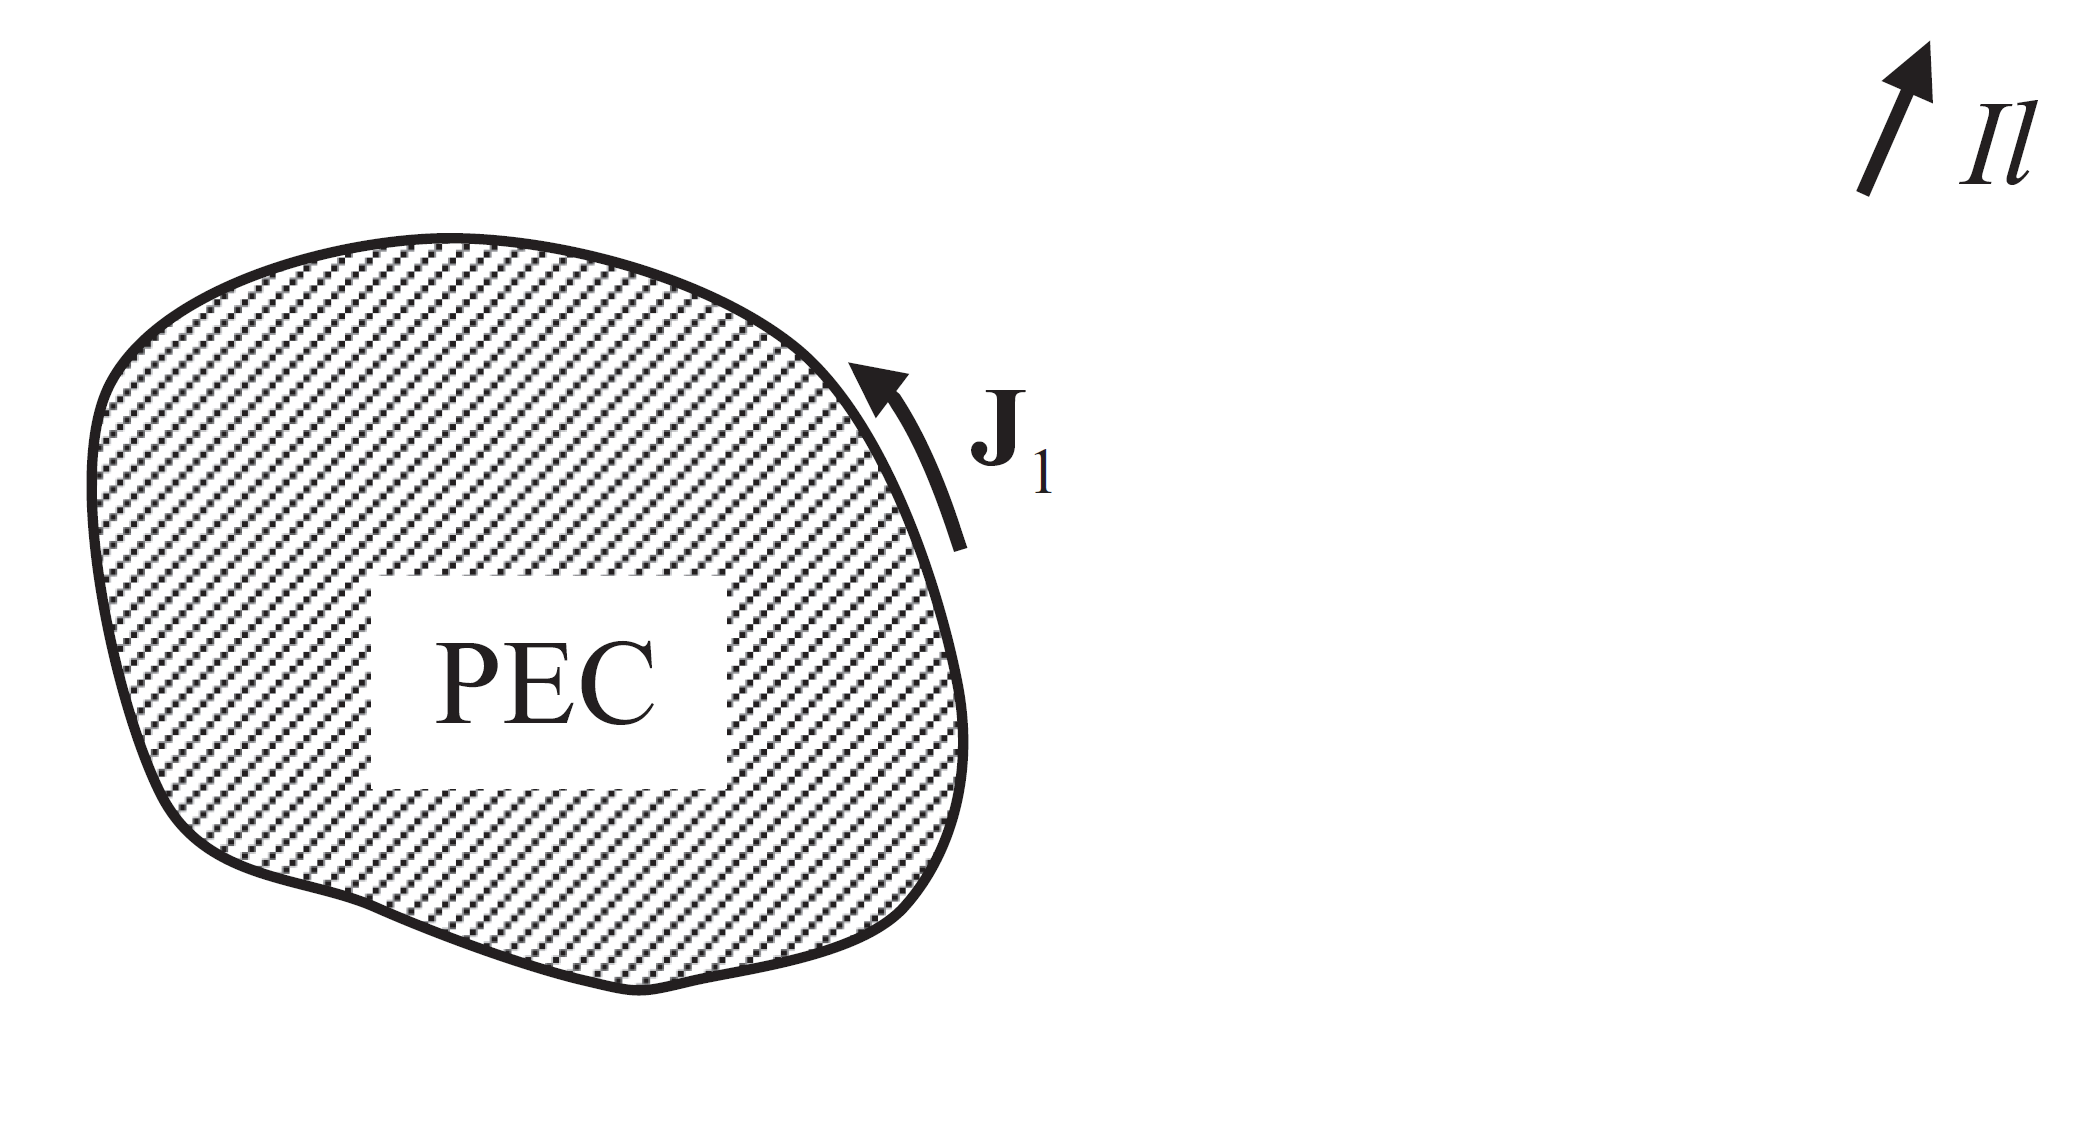
\includegraphics[width=0.25\textwidth]{置于PEC表面的切向电流.PNG}
    \caption{置于PEC表面的切向电流}
    \label{fig:fig12}
\end{figure}
\\根据式\ref{eq:eq206},有
\begin{align}
    \label{eq:eq209}
    \left\langle 1,2\right\rangle =\iiint_V\mathbf{E}_1\cdot\mathbf{J}_2dV=\mathbf{E}_1(\vec{r})\cdot\hat{a}Il
\end{align}
因为$\mathbf{E}_2$在PEC表面满足切向为零的边界条件$\hat{t}\cdot\mathbf{E}_2=0$,根据式\ref{eq:eq207},有
\begin{align}
    \label{eq:eq210}
    \left\langle 2,1\right\rangle =\iiint_V\mathbf{E}_2\cdot\mathbf{J}_1dV=0
\end{align}
根据瑞利-卡森互易定理,$\mathbf{E}_1(\vec{r})\cdot\hat{a}=0$,由于$\vec{r}$和$\hat{a}$任意,所以在任何位置均有$\mathbf{E}_1(\vec{r})=0$,这表明,放置于PEC表面的切向电流不产生辐射场,同理,放置于PMC表面的切向磁流不产生辐射场。\\
(2)考虑一个由单位幅度电流源激励的天线,求其在自由空间中的辐射。除了通过在远场区直接测量其辐射场来确定天线方向图以外,还可以在观察点放置一个方向为$\hat{a}$的无限小电流源$Il$,测量天线激励端的接收电压。把天线激励端看成源1,产生电场$\mathbf{E}_1$,观察点的偶极子看成源2,产生电场$\mathbf{E}_2$,如图\ref{fig:fig13}所示。
\begin{figure}[ht]
    \centering
    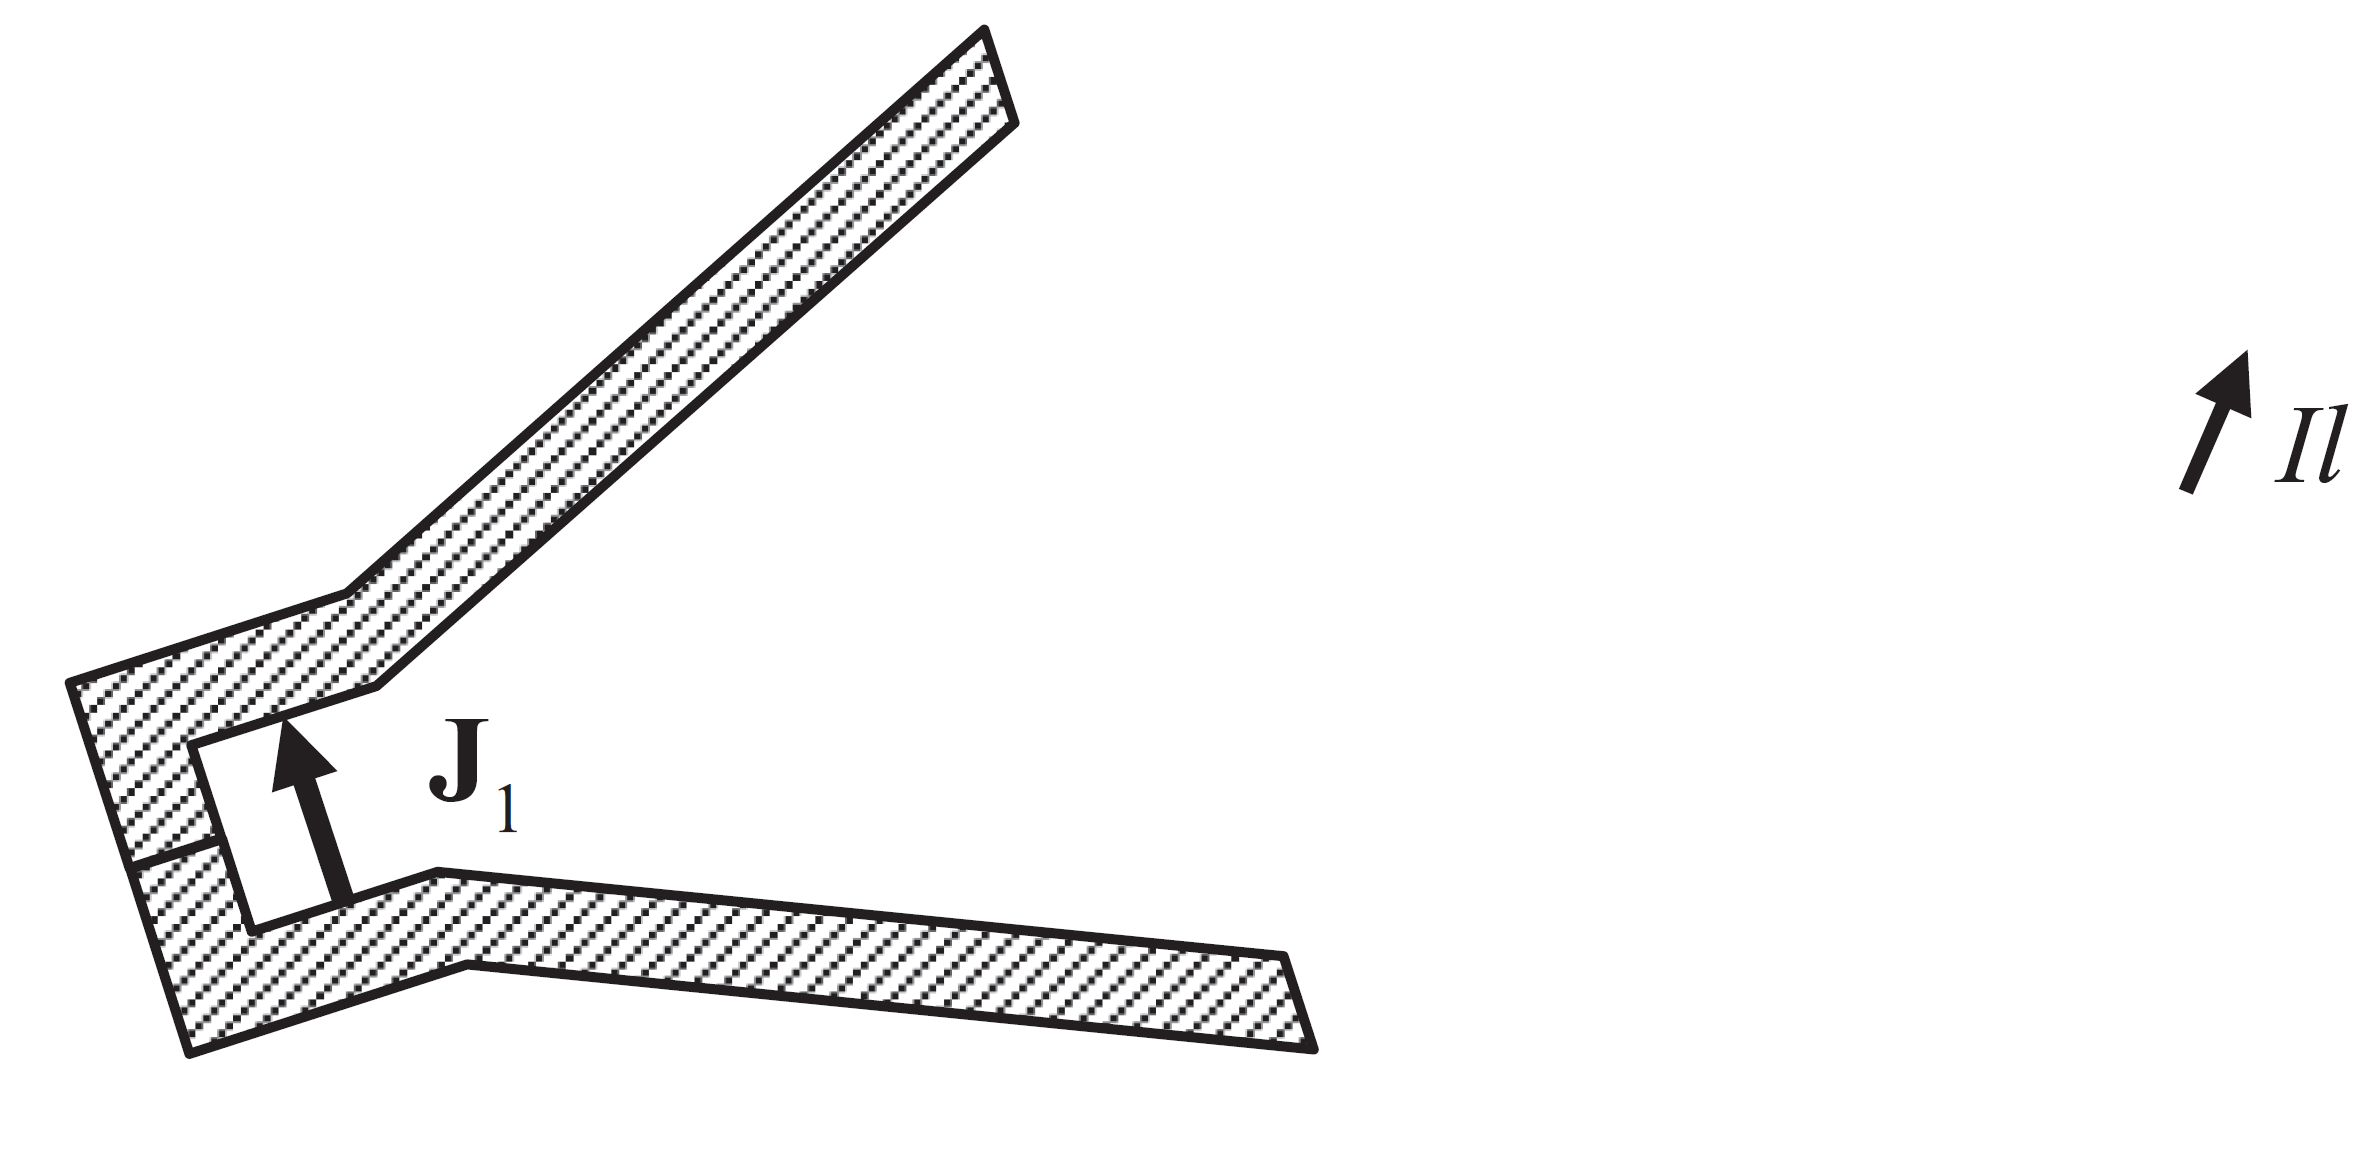
\includegraphics[width=0.25\textwidth]{电流源激励的天线与置于观察点的偶极子.PNG}
    \caption{电流源激励的天线与置于观察点的偶极子}
    \label{fig:fig13}
\end{figure}
\\根据式\ref{eq:eq206},有
\begin{align}
    \label{eq:eq211}
    \left\langle 1,2\right\rangle =\iiint_V\mathbf{E}_1\cdot\mathbf{J}_2dV=\mathbf{E}_1(\vec{r})\cdot\hat{a}Il
\end{align}
根据式\ref{eq:eq207},有
\begin{align}
    \label{eq:eq212}
    \left\langle 2,1\right\rangle =\iiint_V\mathbf{E}_2\cdot\mathbf{J}_1dV=E_2l_1=-V_2
\end{align}
式中$V_2$是接收电压,取决于源2的位置和方向,记为$V_2(\vec{r},\hat{a})$。根据瑞利-卡森互易定理,有
\begin{align}
    \label{eq:eq213}
    \mathbf{E}_1(\vec{r})\cdot\hat{a}=-\frac{V_2(\vec{r},\hat{a})}{Il}
\end{align}
可以通过改变偶极子的位置和方向,并记录天线的接收电压,得到天线的辐射方向图。如果把$\frac{V_2(\vec{r},\hat{a})}{Il}$称为天线的接收方向图,那么上式表明,在互易媒质中,天线的辐射方向图与天线的接收方向图相同。
\subsection{等效原理}
\subsubsection{面等效原理}
假设源被包围在一个虚拟的闭合曲面$S$内,产生场$(\mathbf{E},\mathbf{H})$,如果我们只关心$S$面外的场,那就可以在$S$内放置另外的场$(\mathbf{E}',\mathbf{H}')$来代替原场。如果在$S$上引入面电流和面磁流:
\begin{align}
    \label{eq:eq214}
    \mathbf{J}_S&=\hat{n}\times(\mathbf{H}-\mathbf{H}') \\
    \label{eq:eq215}
    \mathbf{M}_S&=(\mathbf{E}-\mathbf{E}')\times\hat{n}
\end{align}
那么根据边界条件,$\mathbf{J}_S$和$\mathbf{M}_S$将在$S$的外表面产生切向场$\hat{n}\times\mathbf{H}$和$\hat{n}\times\mathbf{E}$,如图\ref{fig:fig14}所示。
那么,对于新问题中的$S$外部区域,与原问题有相同的源(无源)和边界条件,根据唯一性定理,新问题中的$S$外部区域与原问题中的$S$外部区域有相同的场。
\begin{figure}[ht]
    \centering
    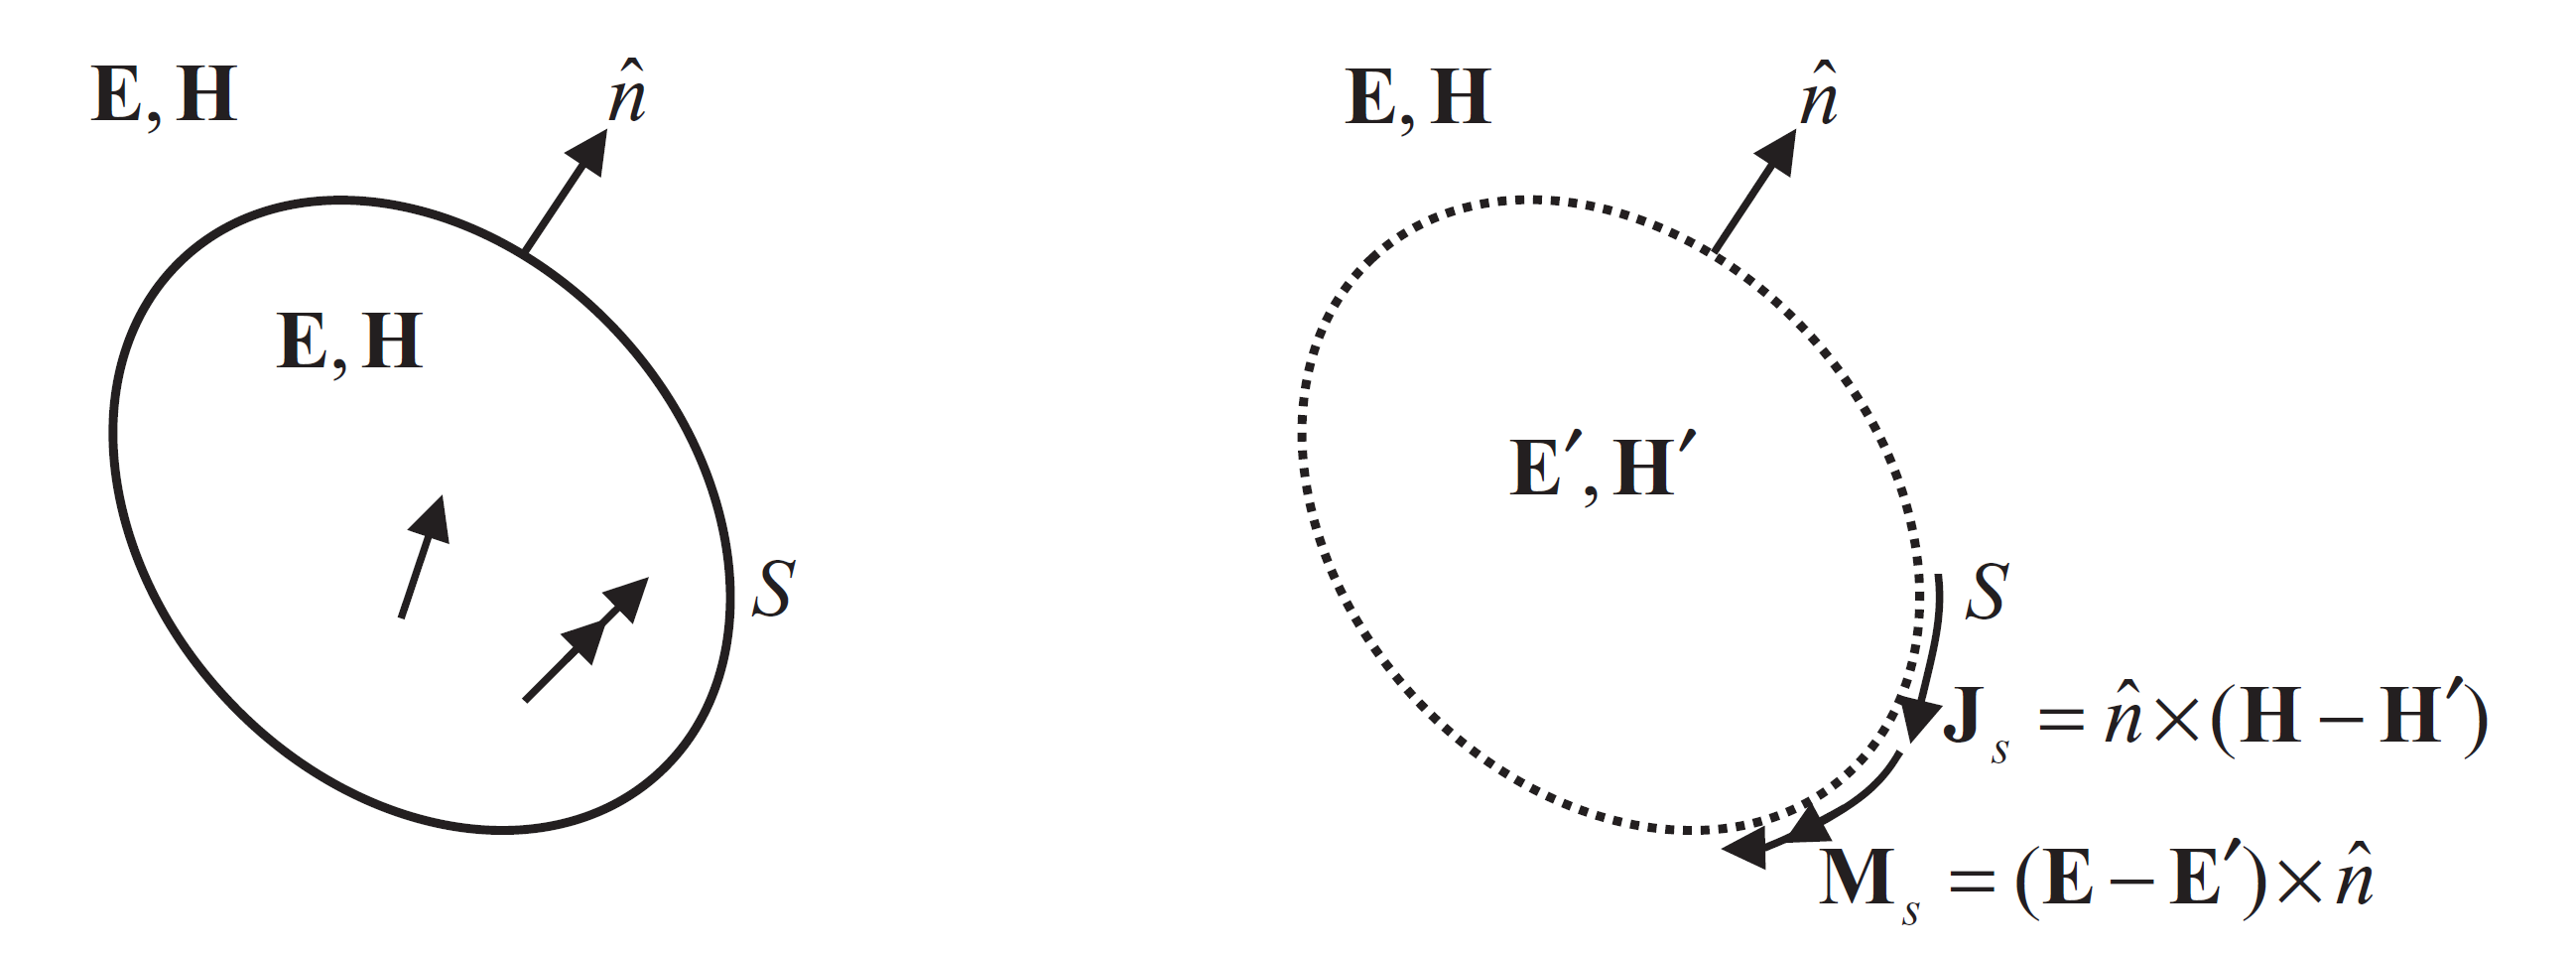
\includegraphics[width=0.5\textwidth]{面等效原理示意图.PNG}
    \caption{面等效原理示意图}
    \label{fig:fig14}
\end{figure}
\par
为简化问题,可令$\mathbf{E}'=0$,$\mathbf{H}'=0$,则等效面电(磁)流为:
\begin{align}
    \label{eq:eq216}
    \mathbf{J}_S&=\hat{n}\times\mathbf{H} \\
    \label{eq:eq217}
    \mathbf{M}_S&=\mathbf{E}\times\hat{n}
\end{align}
此时,在$S$内部填充任何材料都不会对外部区域的场产生影响。如果在$S$内部填充PEC,由上一节内容可知,放置于PEC表面的切向电流不产生辐射场,因此,$S$外部只存在表面磁流$\mathbf{M}_S=\mathbf{E}\times\hat{n}$的辐射场;同理,如果在$S$内部填充PMC,由上一节内容可知,放置于PMC表面的切向磁流不产生辐射场,因此,$S$外部只存在表面电流$\mathbf{J}_S=\hat{n}\times\mathbf{H}$的辐射场,如图\ref{fig:fig28}所示。
\begin{figure}[ht]
    \centering
    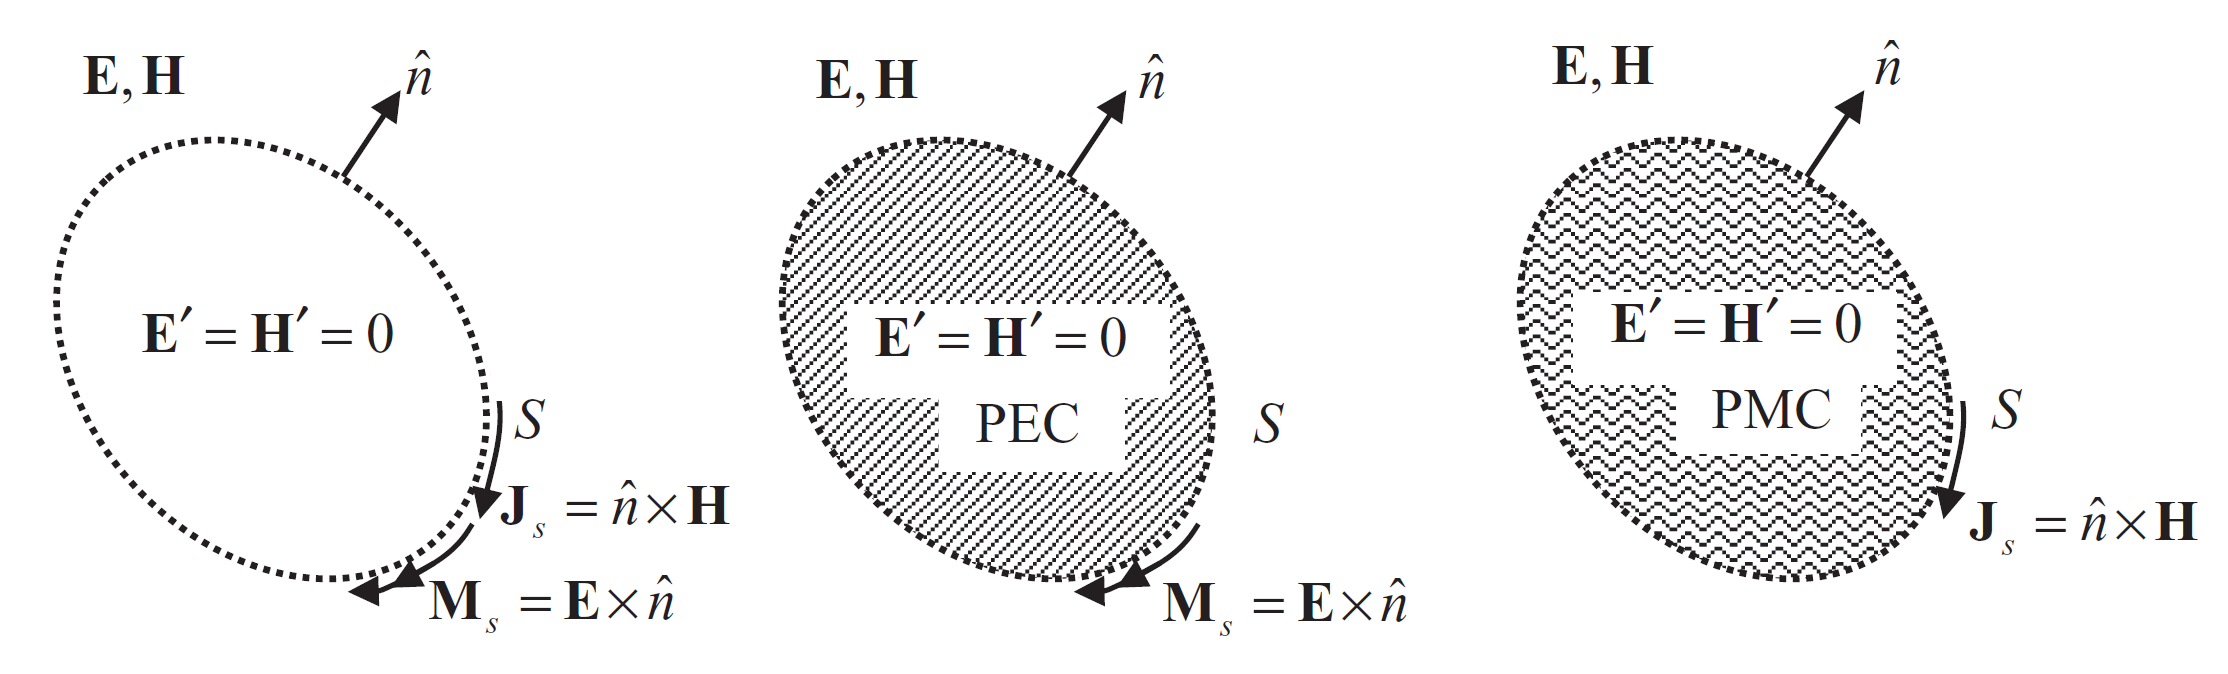
\includegraphics[width=0.5\textwidth]{等效问题.PNG}
    \caption{等效问题}
    \label{fig:fig28}
\end{figure}
\par
如果外区域是介电常数为$\epsilon$、磁导率为$\mu$的无界均匀媒质,则可在$S$内部填充相同的媒质,这样整个空间就是无限大均匀媒质,即自由空间。根据式\ref{eq:eq110}、式\ref{eq:eq111}得,
\begin{align}
    \label{eq:eq218}
    \mathbf{E}(\vec{r})&=-jw\mu\varoiint_S\overline{\mathbf{G}}_{e0}(\vec{r},\vec{r}')\cdot \mathbf{J}_S(\vec{r}')dS'-\varoiint_S\overline{\mathbf{G}}_{m0}(\vec{r},\vec{r}')\cdot \mathbf{M}_S(\vec{r}')dS' \nonumber \\
                       &=-jw\mu\varoiint_S\overline{\mathbf{G}}_{e0}(\vec{r},\vec{r}')\cdot [\hat{n}'\times\mathbf{H}(\vec{r}')]dS'+\varoiint_S\overline{\mathbf{G}}_{m0}(\vec{r},\vec{r}')\cdot [\hat{n}'\times\mathbf{E}(\vec{r}')]dS' \\
    \label{eq:eq219}
    \mathbf{H}(\vec{r})&=-jw\epsilon\varoiint_S\overline{\mathbf{G}}_{e0}(\vec{r},\vec{r}')\cdot \mathbf{M}_S(\vec{r}')dS'+\varoiint_S\overline{\mathbf{G}}_{m0}(\vec{r},\vec{r}')\cdot \mathbf{J}_S(\vec{r}')dS' \nonumber \\
                       &=jw\epsilon\varoiint_S\overline{\mathbf{G}}_{e0}(\vec{r},\vec{r}')\cdot [\hat{n}'\times\mathbf{E}(\vec{r}')]dS'+\varoiint_S\overline{\mathbf{G}}_{m0}(\vec{r},\vec{r}')\cdot [\hat{n}'\times\mathbf{H}(\vec{r}')]dS'
\end{align}
上式(\textbf{\color{blue}{惠更斯原理}}\footnote{波前的每一点发出次波,这些次波互相干涉,叠加形成新的波前。}的数学表示)表明,对于一个包围源的闭合曲面,外区域的场可以由曲面上的切向量分量完全确定,只有当$S$是某特殊形状时,才有解析解。
\subsubsection{等效原理在导体散射问题中的应用}
假设自由空间中存在一个理想导体,源$(\mathbf{J}_i,\mathbf{M}_i)$位于理想导体外部,为了求解源的辐射场,构建一个新的问题:把理想导体移去,用自由空间媒质代替,并假设区域内为零场,保留区域外的源$(\mathbf{J}_i,\mathbf{M}_i)$,根据理想导体的边界条件,$\hat{n}\times\mathbf{H}=\mathbf{J}_S$,$\hat{n}\times\mathbf{E}=0$,引入等效面电流$\mathbf{J}_S=\hat{n}\times\mathbf{H}$,而无需引入等效面磁流。如图\ref{fig:fig17}所示,原问题等效为一个源$(\mathbf{J}_i,\mathbf{M}_i)$和面电流$\mathbf{J}_S$在自由空间的辐射问题。
\begin{figure}[ht]
    \centering
    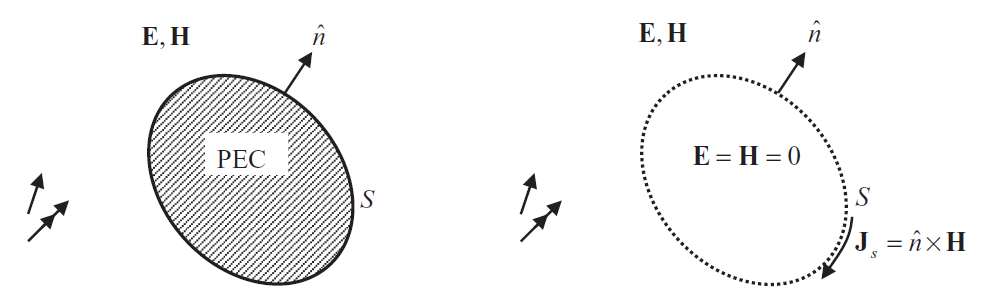
\includegraphics[width=0.5\textwidth]{理想导体散射的物理等效示意图.PNG}
    \caption{理想导体散射的物理等效示意图}
    \label{fig:fig17}
\end{figure}
\par
根据式\ref{eq:eq110}、式\ref{eq:eq111}得,
\begin{align}
    \label{eq:eq220}
    \mathbf{E}(\vec{r})&=-jw\mu\iiint_{V_S}\overline{\mathbf{G}}_{e0}(\vec{r},\vec{r}')\cdot \mathbf{J}_i(\vec{r}')dV'-\iiint_{V_S}\overline{\mathbf{G}}_{m0}(\vec{r},\vec{r}')\cdot \mathbf{M}_i(\vec{r}')dV' \nonumber \\
                       &\qquad-jw\mu\varoiint_S\overline{\mathbf{G}}_{e0}(\vec{r},\vec{r}')\cdot \mathbf{J}_S(\vec{r}')dS' \nonumber \\
                       &=\mathbf{E}^{inc}-jw\mu\varoiint_S\overline{\mathbf{G}}_{e0}(\vec{r},\vec{r}')\cdot [\hat{n}'\times\mathbf{H}(\vec{r}')]dS' \\
    \label{eq:eq221}
    \mathbf{H}(\vec{r})&=-jw\epsilon\iiint_{V_S}\overline{\mathbf{G}}_{e0}(\vec{r},\vec{r}')\cdot \mathbf{M}_i(\vec{r}')dV'+\iiint_{V_S}\overline{\mathbf{G}}_{m0}(\vec{r},\vec{r}')\cdot \mathbf{J}_i(\vec{r}')dV' \nonumber \\
                       &\qquad+\varoiint_S\overline{\mathbf{G}}_{m0}(\vec{r},\vec{r}')\cdot \mathbf{J}_S(\vec{r}')dS' \nonumber \\
                       &=\mathbf{H}^{inc}+\varoiint_S\overline{\mathbf{G}}_{m0}(\vec{r},\vec{r}')\cdot [\hat{n}'\times\mathbf{H}(\vec{r}')]dS'
\end{align}
式中,$V_S$是源存在的区域,
\begin{align}
    \label{eq:eq222}
    \mathbf{E}^{inc}&=-jw\mu\iiint_{V_S}\overline{\mathbf{G}}_{e0}(\vec{r},\vec{r}')\cdot \mathbf{J}_i(\vec{r}')dV'-\iiint_{V_S}\overline{\mathbf{G}}_{m0}(\vec{r},\vec{r}')\cdot \mathbf{M}_i(\vec{r}')dV' \\
    \label{eq:eq223}
    \mathbf{H}^{inc}&=-jw\epsilon\iiint_{V_S}\overline{\mathbf{G}}_{e0}(\vec{r},\vec{r}')\cdot \mathbf{M}_i(\vec{r}')dV'+\iiint_{V_S}\overline{\mathbf{G}}_{m0}(\vec{r},\vec{r}')\cdot \mathbf{J}_i(\vec{r}')dV'
\end{align}
是源$(\mathbf{J}_i,\mathbf{M}_i)$产生的场,称为\textbf{\color{blue}{入射场}}。\par
被积函数中$S$面上的场在实际中是未知的,所以不能直接利用式\ref{eq:eq220}、式\ref{eq:eq221}求得电磁场(可通过矩量法求解积分方程)。因为这里的等效面电流是物理上的真实面电流,所以上述等效称为\textbf{\color{blue}{物理等效}}。\par
当物体尺寸与入射波的波长相比很大时,可以求得近似解。当入射场的源距离散射体很远时,入射波可看成平面波;当物体和波长相比很大时,对于每一个场点,散射体表面可以看成无限大平面;而当平面波入射到无限大PEC平面时,其表面感应电流为$\mathbf{J}_S=2\hat{n}\times\mathbf{H}^{inc}$。因此,对于电大尺寸的物体,可以近似认为亮区感应电流为$\mathbf{J}_S\approx2\hat{n}\times\mathbf{H}^{inc}$,而暗区感应电流为0,如图\ref{fig:fig18}所示,这种近似称为\textbf{\color{blue}{物理光学近似}}。
\begin{figure}[ht]
    \centering
    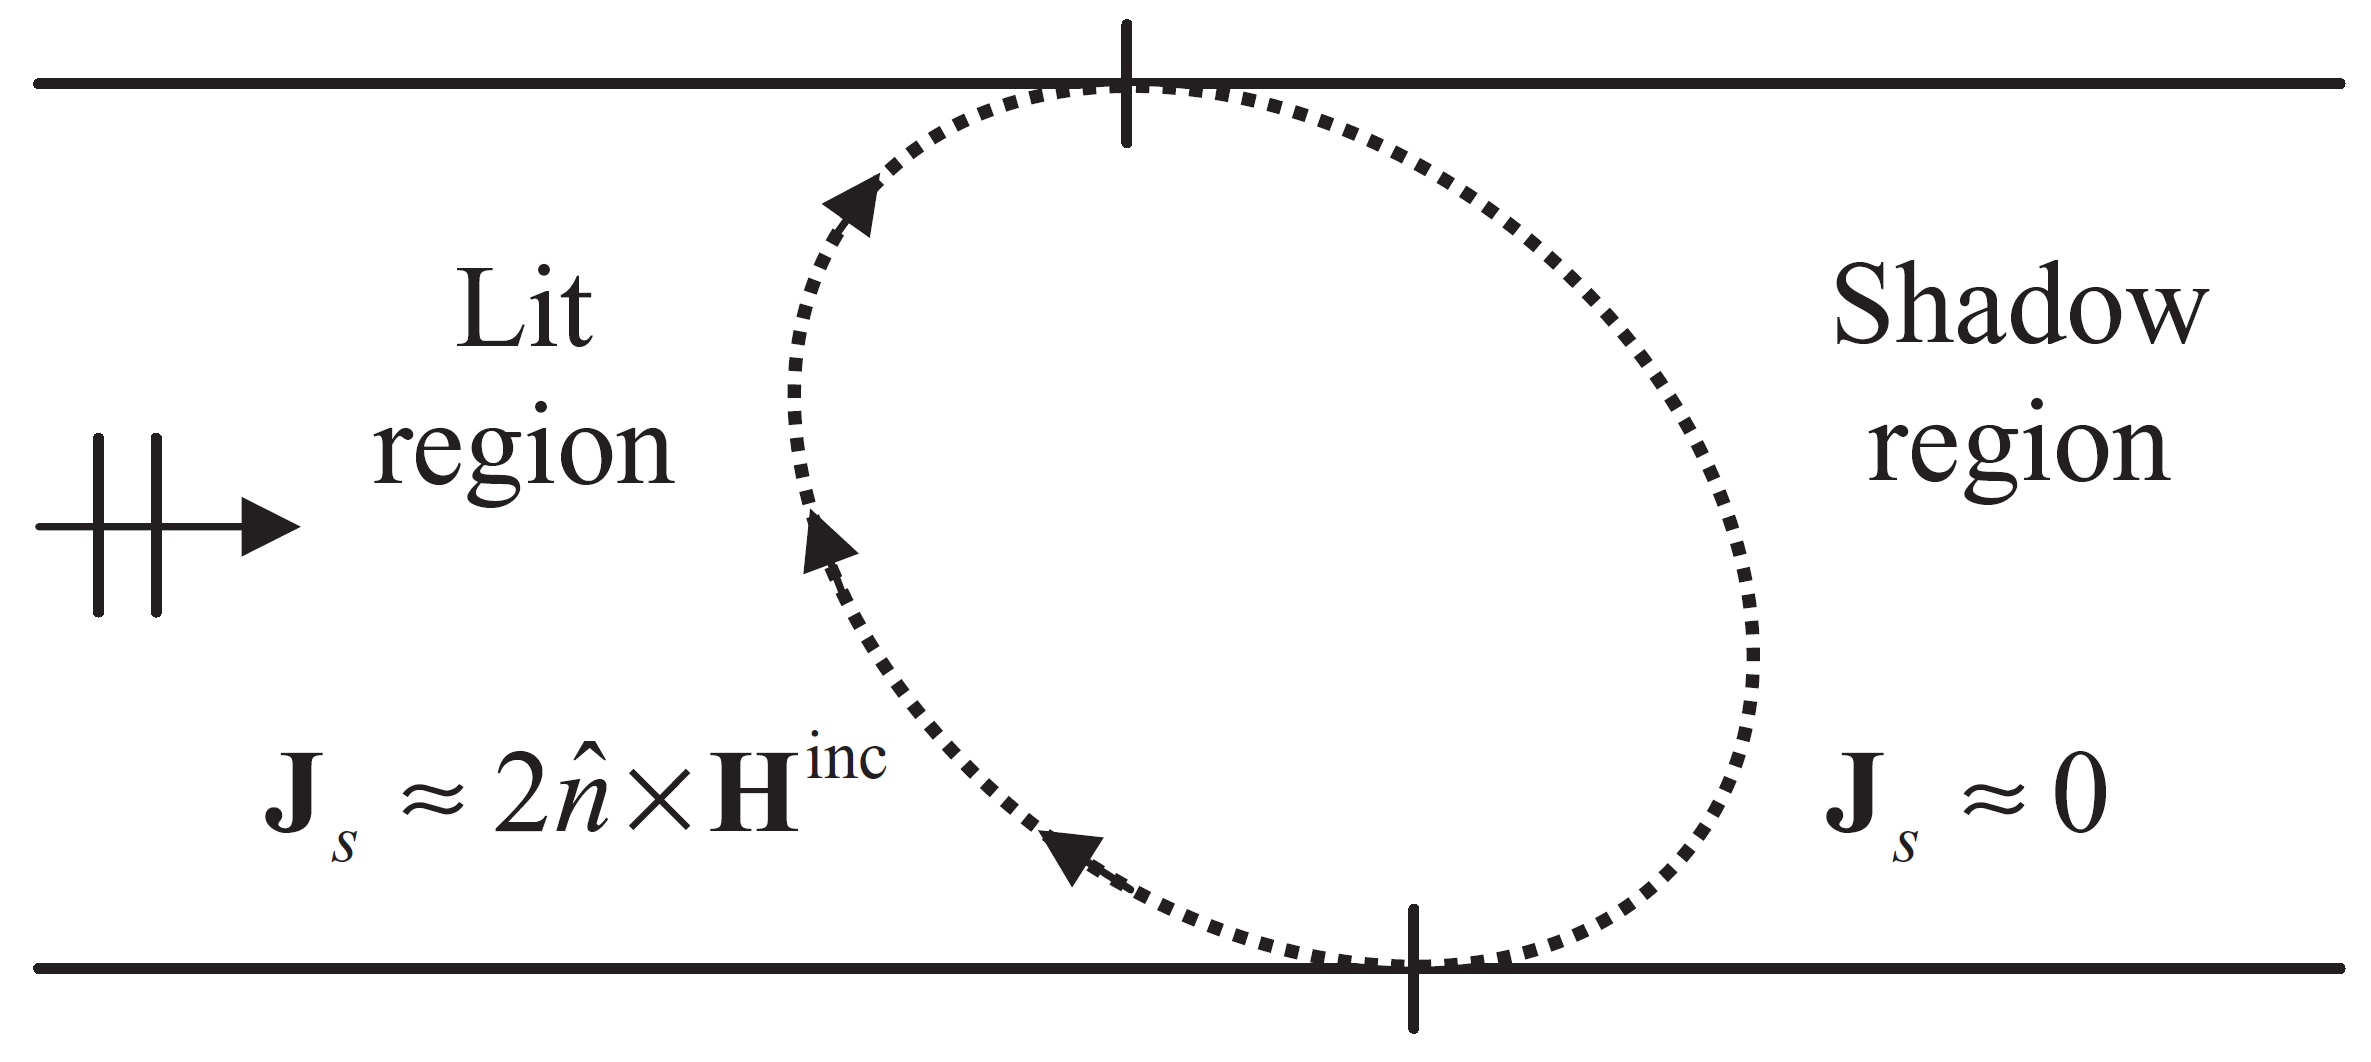
\includegraphics[width=0.4\textwidth]{物理光学近似示意图.PNG}
    \caption{物理光学近似示意图}
    \label{fig:fig18}
\end{figure}
\\因此,式\ref{eq:eq220}、式\ref{eq:eq221}重写为:
\begin{align}
    \label{eq:eq224}
    \mathbf{E}(\vec{r})&\approx\mathbf{E}^{inc}(\vec{r})-2jw\mu\varoiint_{S_{lit}}\overline{\mathbf{G}}_{e0}(\vec{r},\vec{r}')\cdot [\hat{n}'\times\mathbf{H}^{inc}(\vec{r}')]dS' \\
    \label{eq:eq225}
    \mathbf{H}(\vec{r})&\approx\mathbf{H}^{inc}(\vec{r})+2\varoiint_{S_{lit}}\overline{\mathbf{G}}_{m0}(\vec{r},\vec{r}')\cdot [\hat{n}'\times\mathbf{H}^{inc}(\vec{r}')]dS'
\end{align}
式中,$S_{lit}$是$S$在亮区的部分。\par
上述物理等效中,等效面电流由总场决定,因此是未知的。现保留导体,构造新的等效问题。
\par
定义\textbf{\color{blue}{散射场}}为总场和入射场的差值,即
\begin{align}
    \label{eq:eq226}
    \mathbf{E}^{sc}(\vec{r})&=\mathbf{E}(\vec{r})-\mathbf{E}^{inc}(\vec{r}) \\
    \label{eq:eq227}
    \mathbf{H}^{sc}(\vec{r})&=\mathbf{H}(\vec{r})-\mathbf{H}^{inc}(\vec{r})
\end{align}
散射场由导体上的感应电(磁)流产生,为了产生这样的散射场,需要引入的等效电(磁)流为:
\begin{align}
    \label{eq:eq228}
    \mathbf{J}_S&=\hat{n}\times\mathbf{H}^{sc} \\
    \label{eq:eq229}
    \mathbf{M}_S&=\mathbf{E}^{sc}\times\hat{n}
\end{align}
也就是说,仅在$S$外区域构建散射场,之后计算总场时直接在散射场的基础上增加入射场。由于$\mathbf{J}_S$在PEC表面不辐射,辐射场进来自于$\mathbf{M}_S$,此外,由理想导体的边界条件,有$\hat{n}\times\mathbf{E}=0$,即总场在导体边界的切向分量为零,代入式\ref{eq:eq229},
\begin{align}
    \label{eq:eq230}
    \mathbf{M}_S=(\mathbf{E}-\mathbf{E}^{inc})\times\hat{n}=\hat{n}\times\mathbf{E}^{inc}
\end{align}
此时,等效面磁流仅由入射场决定,是已知的。这种面等效原理称为\textbf{\color{blue}{感应定理}},如图\ref{fig:fig19}所示。
\begin{figure}[ht]
    \centering
    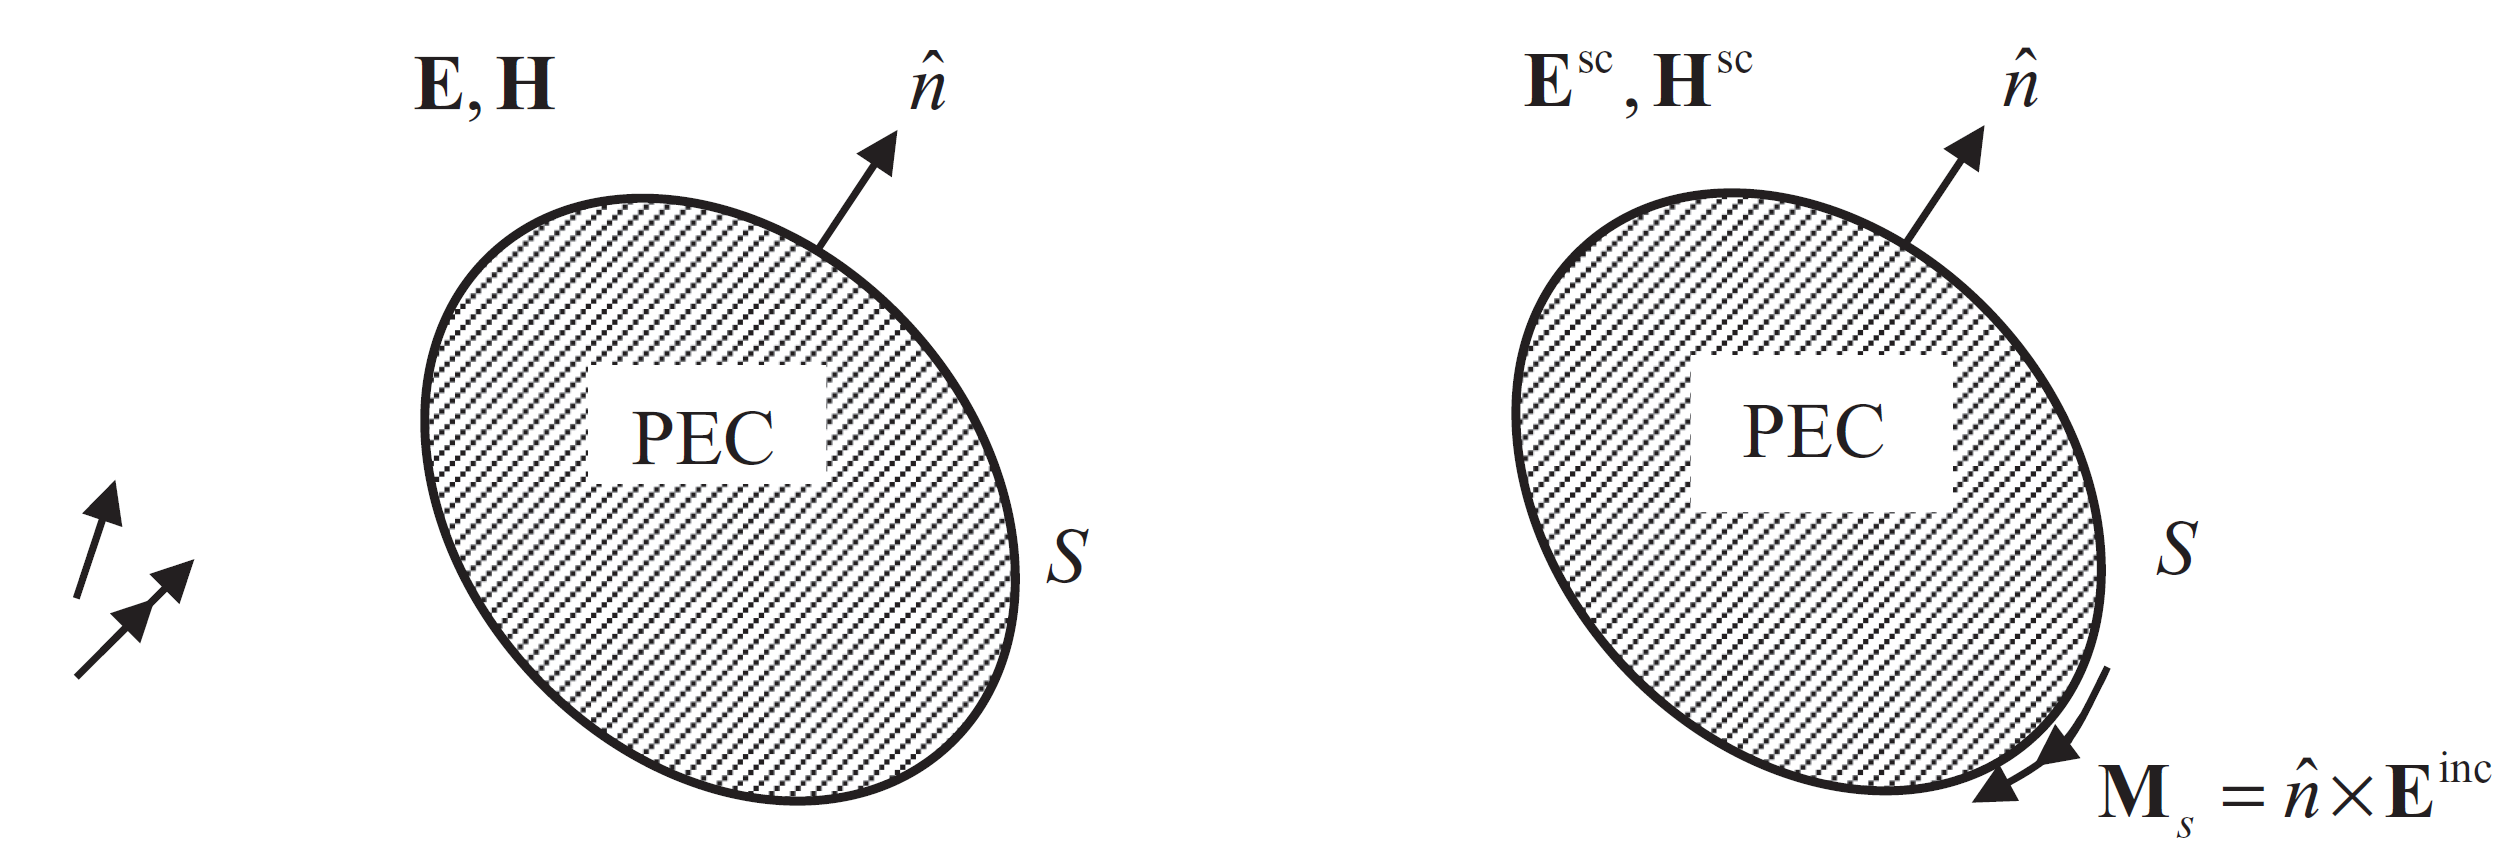
\includegraphics[width=0.6\textwidth]{导体散射的感应定理示意图.PNG}
    \caption{导体散射的感应定理示意图}
    \label{fig:fig19}
\end{figure}
对于电大尺寸的物体,对位于物体表面的磁流来说,表面可以近似看成无限大平面,因此可以应用镜像原理将问题转换为自由空间问题,如图\ref{fig:fig20}所示,此时观察点的一侧表面上的等效磁流变为$\mathbf{M}_S\approx2\hat{n}\times\mathbf{E}^{inc}$,观察点另一侧表面上的等效磁流辐射忽略不计。
\begin{figure}[ht]
    \centering
    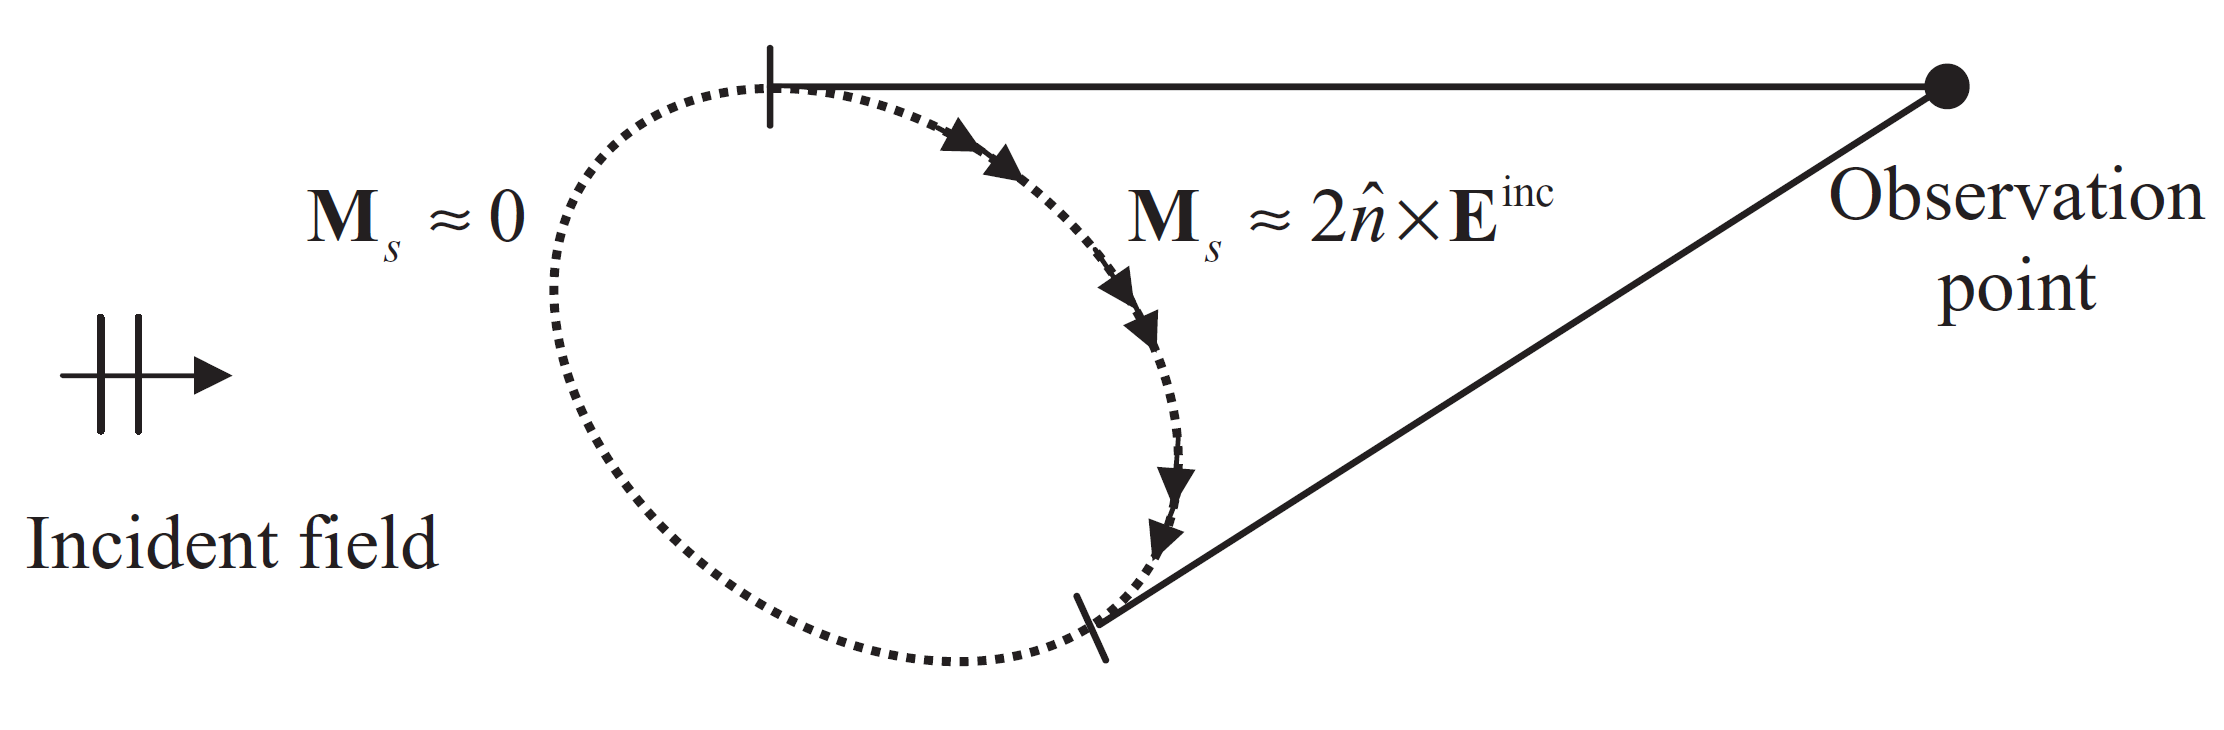
\includegraphics[width=0.6\textwidth]{感应定理的镜像原理近似示意图.PNG}
    \caption{感应定理的镜像原理近似示意图}
    \label{fig:fig20}
\end{figure}
\par
根据式\ref{eq:eq110}、式\ref{eq:eq111}得,
\begin{align}
    \label{eq:eq231}
    \mathbf{E}(\vec{r})&\approx\mathbf{E}^{inc}(\vec{r})-2\varoiint_{S_{obs}}\overline{\mathbf{G}}_{m0}(\vec{r},\vec{r}')\cdot [\hat{n}'\times\mathbf{E}^{inc}(\vec{r}')]dS' \\
    \label{eq:eq232}
    \mathbf{H}(\vec{r})&\approx\mathbf{H}^{inc}(\vec{r})-2jw\epsilon\varoiint_{S_{obs}}\overline{\mathbf{G}}_{e0}(\vec{r},\vec{r}')\cdot [\hat{n}'\times\mathbf{E}^{inc}(\vec{r}')]dS'
\end{align}
式中,$S_{obs}$是$S$面在观察点$\vec{r}$一侧能看到的部分。
\subsubsection{等效原理在介质体散射中的应用}
考虑一个介质体,处于介电常数为$\epsilon_1$,磁导率为$\mu_1$的空间中,介质体的介电常数为$\epsilon_2$,磁导率为$\mu_2$,如图\ref{fig:fig21}所示。
\begin{figure}[ht]
    \centering
    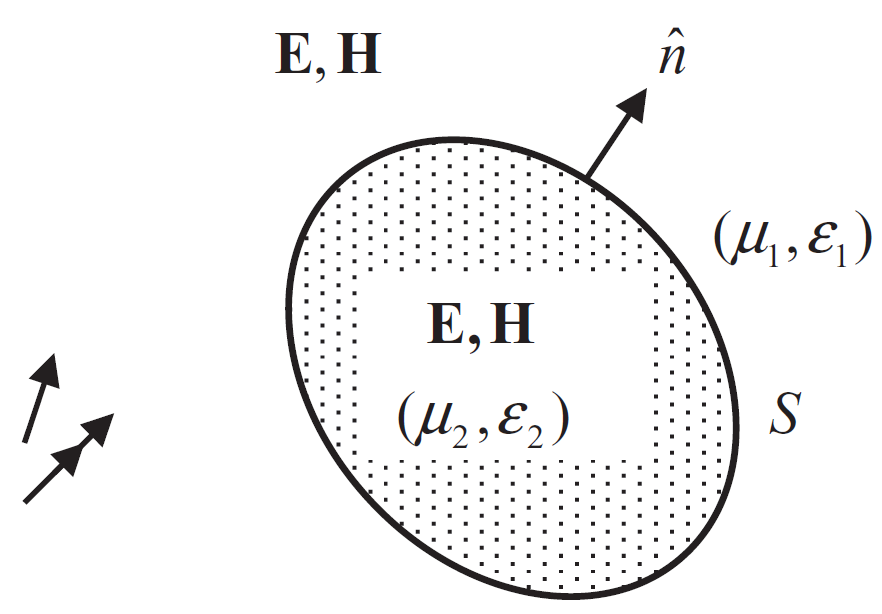
\includegraphics[width=0.3\textwidth]{介质体散射的原问题.PNG}
    \caption{介质体散射的原问题}
    \label{fig:fig21}
\end{figure}
\\
首先构建外区域的等效问题,设内区域为零场,外区域与原问题相同,用外区域的媒质填充内区域,即$\mu_1$、$\epsilon_1$,等效面电(磁)流同式\ref{eq:eq216}、式\ref{eq:eq217},因此外区域场等效为源与面电(磁)流在自由空间中的叠加场,如图\ref{fig:fig22}所示。
\begin{figure}[ht]
    \centering
    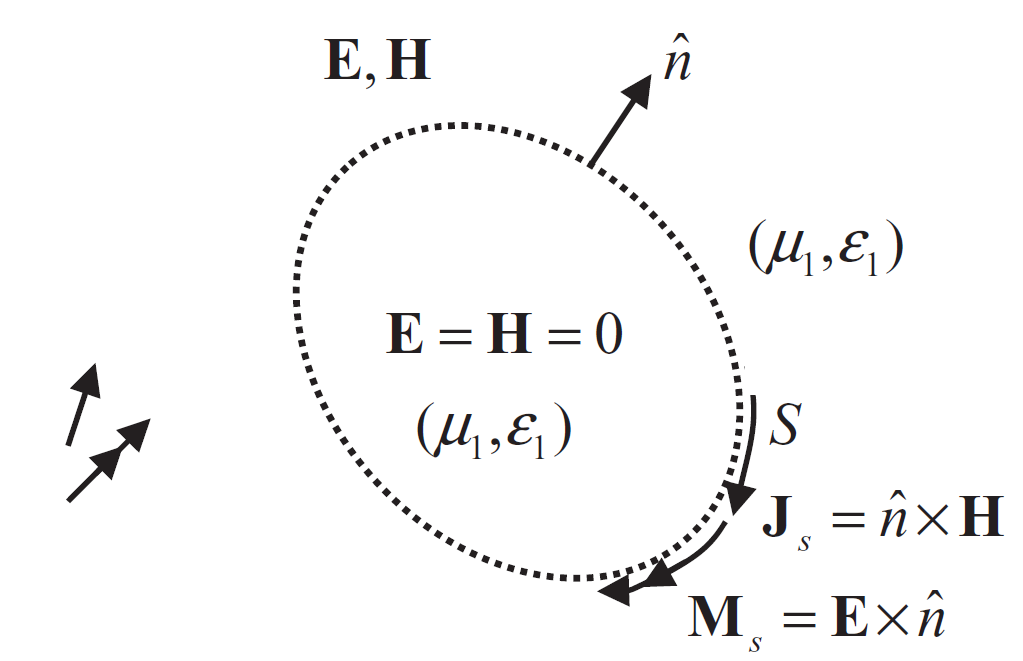
\includegraphics[width=0.3\textwidth]{介质体散射的外部场等效问题.PNG}
    \caption{介质体散射的外部场等效问题}
    \label{fig:fig22}
\end{figure}
\\
根据式\ref{eq:eq110}、式\ref{eq:eq111},此时外区域电磁场为:
\begin{align}
    \label{eq:eq233}
    \mathbf{E}(\vec{r})&=\mathbf{E}^{inc}-jw\mu_1\varoiint_S\overline{\mathbf{G}}_{e0}(\vec{r},\vec{r}';k_1)\cdot\mathbf{J}_S(\vec{r}')dS'-\varoiint_S\overline{\mathbf{G}}_{m0}(\vec{r},\vec{r}';k_1)\cdot\mathbf{M}_S(\vec{r}')dS' \\
    \label{eq:eq234}
    \mathbf{H}(\vec{r})&=\mathbf{H}^{inc}-jw\epsilon_1\varoiint_S\overline{\mathbf{G}}_{e0}(\vec{r},\vec{r}';k_1)\cdot\mathbf{M}_S(\vec{r}')dS'+\varoiint_S\overline{\mathbf{G}}_{m0}(\vec{r},\vec{r}';k_1)\cdot\mathbf{J}_S(\vec{r}')dS'
\end{align}
其中波数为$k_1=w\sqrt{\mu_1\epsilon_1}$。\\
其次考虑构建内区域的等效问题,设外区域为零场,内区域与原问题相同,用内区域的媒质填充外区域,即$\mu_2$、$\epsilon_2$,等效面电(磁)流为:
\begin{align}
    \label{eq:eq235}
    \tilde{\mathbf{J}}_S&=-\hat{n}\times\mathbf{H} \\
    \label{eq:eq236}
    \tilde{\mathbf{M}}_S&=-\mathbf{E}\times\hat{n}
\end{align}
因此内区域场等效为面电(磁)流在自由空间中产生的场,如图\ref{fig:fig23}所示。
\begin{figure}[ht]
    \centering
    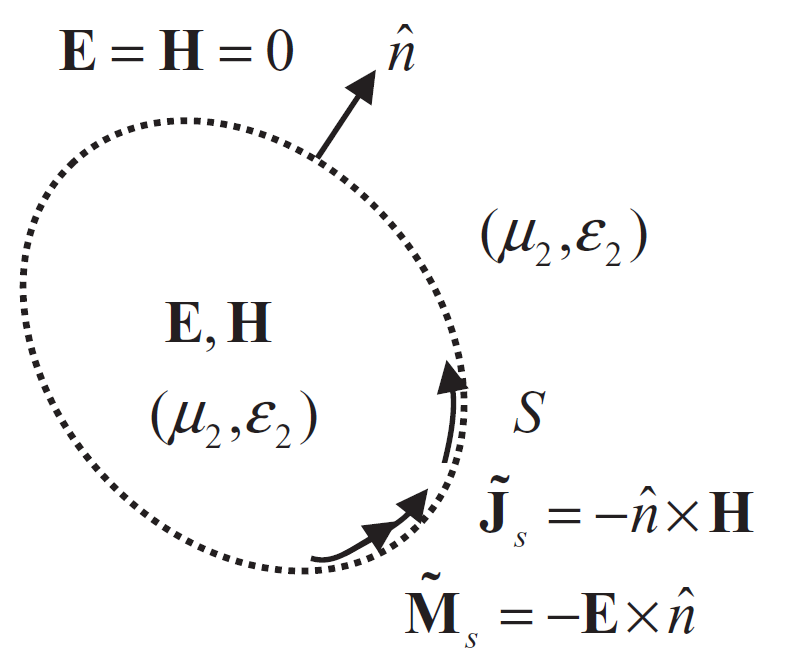
\includegraphics[width=0.25\textwidth]{介质体散射的内部场等效问题.PNG}
    \caption{介质体散射的内部场等效问题}
    \label{fig:fig23}
\end{figure}
\\
根据式\ref{eq:eq110}、式\ref{eq:eq111},此时内区域电磁场为:
\begin{align}
    \label{eq:eq237}
    \mathbf{E}(\vec{r})&=-jw\mu_2\varoiint_S\overline{\mathbf{G}}_{e0}(\vec{r},\vec{r}';k_2)\cdot\tilde{\mathbf{J}}_S(\vec{r}')dS'-\varoiint_S\overline{\mathbf{G}}_{m0}(\vec{r},\vec{r}';k_2)\cdot\tilde{\mathbf{M}}_S(\vec{r}')dS' \\
    \label{eq:eq238}
    \mathbf{H}(\vec{r})&=-jw\epsilon_2\varoiint_S\overline{\mathbf{G}}_{e0}(\vec{r},\vec{r}';k_2)\cdot\tilde{\mathbf{M}}_S(\vec{r}')dS'+\varoiint_S\overline{\mathbf{G}}_{m0}(\vec{r},\vec{r}';k_2)\cdot\tilde{\mathbf{J}}_S(\vec{r}')dS'
\end{align}
其中波数为$k_2=w\sqrt{\mu_2\epsilon_2}$。\par
式\ref{eq:eq233}、式\ref{eq:eq234}、式\ref{eq:eq237}、式\ref{eq:eq238}不能直接计算场,因为等效电(磁)流源未知,但可以用于构建积分方程,求解等效电(磁)流源。\par
也可用感应定理构建等效问题,保留散射体,在内区域产生总场,在外区域产生散射场,如图\ref{fig:fig24}所示。
\begin{figure}[ht]
    \centering
    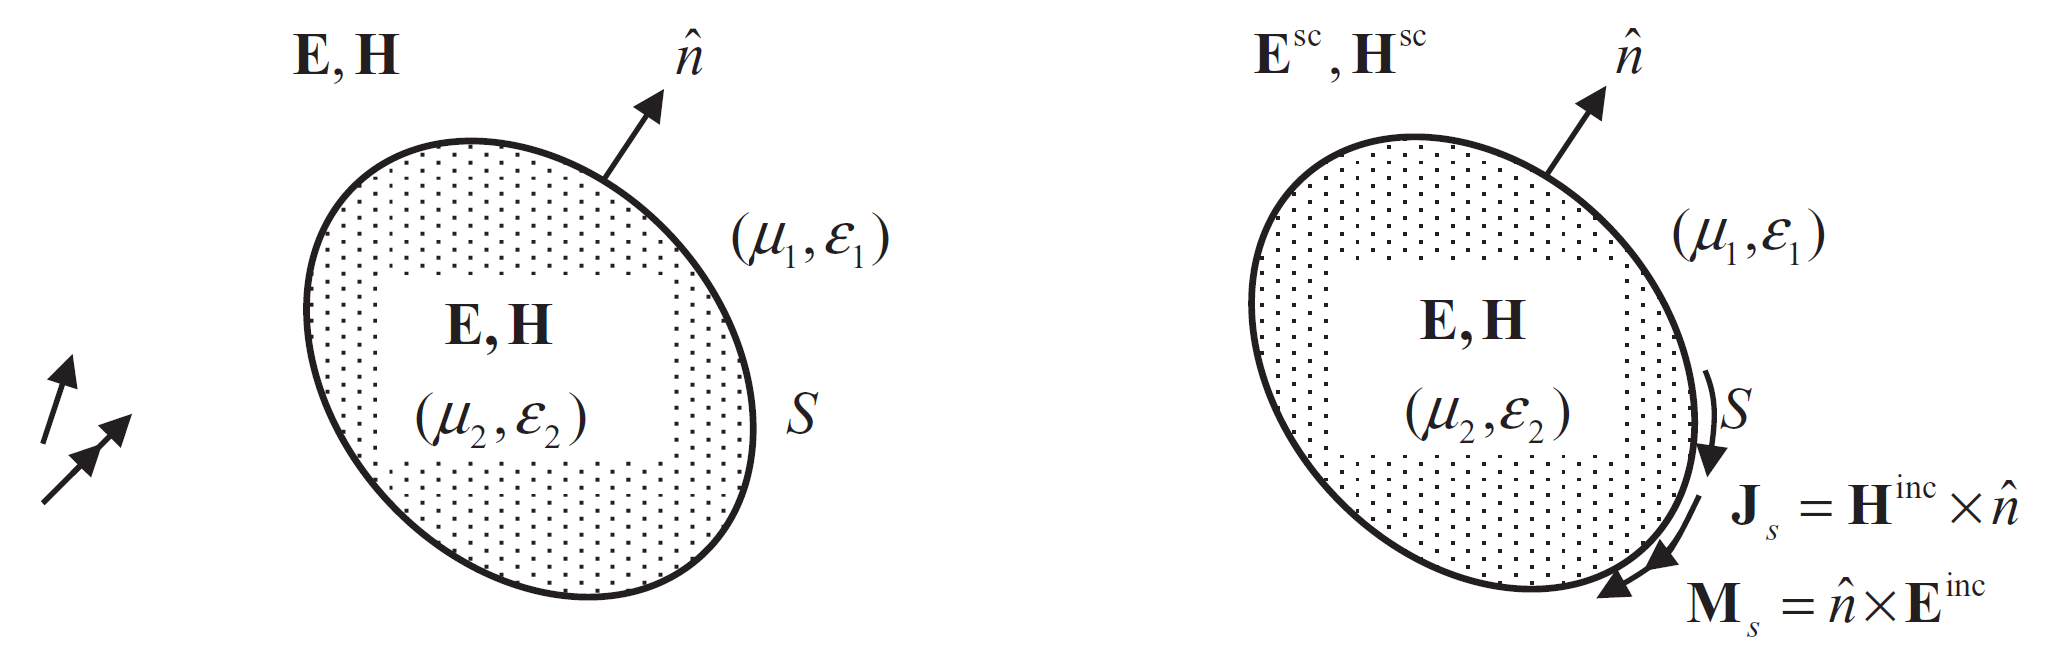
\includegraphics[width=0.5\textwidth]{介质体散射的感应定理示意图.PNG}
    \caption{介质体散射的感应定理示意图}
    \label{fig:fig24}
\end{figure}
\\引入等效电(磁)流:
\begin{align}
    \label{eq:eq239}
    \mathbf{J}_S&=\hat{n}\times(\mathbf{H}^{sc}-\mathbf{H})=-\hat{n}\times\mathbf{H}^{inc} \\
    \label{eq:eq240}
    \mathbf{M}_S&=(\mathbf{E}^{sc}-\mathbf{E})\times\hat{n}=-\mathbf{E}^{inc}\times\hat{n}
\end{align}
此时电(磁)流源已知,但由于介质的存在,无法使用自由空间的场-源关系计算,因此这种方法不实用。
\subsubsection{体等效原理}
考虑源$(\mathbf{J}_i,\mathbf{M}_i)$,以及介电常数为$\tilde{\epsilon}$、磁导率为$\tilde{\mu}$的物体同时处于介电常数为$\epsilon$、磁导率为$\mu$的自用空间中。辐射场满足麦克斯韦方程组:
\begin{align}
    \label{eq:eq241}
    \nabla\times\mathbf{E}&=-jw\mu(\vec{r})\mathbf{H}-\mathbf{M}_i \nonumber \\
                          &=-jw\mu\mathbf{H}-\mathbf{M}_{eq}-\mathbf{M}_i \\
    \label{eq:eq242}
    \nabla\times\mathbf{H}&=jw\epsilon(\vec{r})\mathbf{E}+\mathbf{J}_i \nonumber \\
                          &=jw\epsilon\mathbf{E}+\mathbf{J}_{eq}+\mathbf{J}_i
\end{align}
其中
\begin{align}
    \label{eq:eq243}
    \mu(\vec{r})&=
    \left\{
        \begin{array}{lr}
            \tilde{\mu}, &\vec{r}\in V_O \\
            \mu,         &\vec{r}\notin V_O
        \end{array}
    \right. \\
    \label{eq:eq244}
    \epsilon(\vec{r})&=
    \left\{
        \begin{array}{lr}
            \tilde{\epsilon}, &\vec{r}\in V_O \\
            \epsilon,         &\vec{r}\notin V_O
        \end{array}
    \right.
\end{align}
$V_O$代表物体所占空间。式\ref{eq:eq241}、式\ref{eq:eq242}中,
\begin{align}
    \label{eq:eq245}
    \mathbf{M}_{eq}&=jw[\mu(\vec{r})-\mu]\mathbf{H} \\
    \label{eq:eq246}
    \mathbf{J}_{eq}&=jw[\epsilon(\vec{r})-\epsilon]\mathbf{E}
\end{align}
则式\ref{eq:eq241}、式\ref{eq:eq242}表示源$(\mathbf{J}_i,\mathbf{M}_i,\mathbf{J}_{eq},\mathbf{M}_{eq})$在自由空间中的辐射场所满足的麦克斯韦方程组。由自由空间中的场-源关系,即式\ref{eq:eq110}、式\ref{eq:eq111}得,
\begin{align}
    \label{eq:eq247}
    \mathbf{E}(\vec{r})&=-jw\mu\iiint_{V_S}\overline{\mathbf{G}}_{e0}(\vec{r},\vec{r}')\cdot \mathbf{J}_i(\vec{r}')dV'-\iiint_{V_S}\overline{\mathbf{G}}_{m0}(\vec{r},\vec{r}')\cdot \mathbf{M}_i(\vec{r}')dV' \nonumber \\
                       &\qquad-jw\mu\iiint_{V_O}\overline{\mathbf{G}}_{e0}(\vec{r},\vec{r}')\cdot \mathbf{J}_{eq}(\vec{r}')dV'-\iiint_{V_O}\overline{\mathbf{G}}_{m0}(\vec{r},\vec{r}')\cdot \mathbf{M}_{eq}(\vec{r}')dV' \nonumber \\
                       &=\mathbf{E}^{inc}(\vec{r})-jw\mu\iiint_{V_O}\overline{\mathbf{G}}_{e0}(\vec{r},\vec{r}')\cdot \mathbf{J}_{eq}(\vec{r}')dV'-\iiint_{V_O}\overline{\mathbf{G}}_{m0}(\vec{r},\vec{r}')\cdot \mathbf{M}_{eq}(\vec{r}')dV' \nonumber \\
                       &=\mathbf{E}^{inc}(\vec{r})+w^2\mu\iiint_{V_O}\overline{\mathbf{G}}_{e0}(\vec{r},\vec{r}')\cdot (\tilde{\epsilon}-\epsilon)\mathbf{E}(\vec{r}')dV'-jw\iiint_{V_O}\overline{\mathbf{G}}_{m0}(\vec{r},\vec{r}')\cdot (\tilde{\mu}-\mu)\mathbf{H}(\vec{r}')dV'  \\
    \label{eq:eq248}
    \mathbf{H}(\vec{r})&=-jw\epsilon\iiint_{V_S}\overline{\mathbf{G}}_{e0}(\vec{r},\vec{r}')\cdot \mathbf{M}_i(\vec{r}')dV'+\iiint_{V_S}\overline{\mathbf{G}}_{m0}(\vec{r},\vec{r}')\cdot \mathbf{J}_i(\vec{r}')dV' \nonumber \\
                       &\qquad-jw\epsilon\iiint_{V_O}\overline{\mathbf{G}}_{e0}(\vec{r},\vec{r}')\cdot \mathbf{M}_{eq}(\vec{r}')dV'+\iiint_{V_O}\overline{\mathbf{G}}_{m0}(\vec{r},\vec{r}')\cdot \mathbf{J}_{eq}(\vec{r}')dV' \nonumber \\
                       &=\mathbf{H}^{inc}(\vec{r})-jw\epsilon\iiint_{V_O}\overline{\mathbf{G}}_{e0}(\vec{r},\vec{r}')\cdot \mathbf{M}_{eq}(\vec{r}')dV'+\iiint_{V_O}\overline{\mathbf{G}}_{m0}(\vec{r},\vec{r}')\cdot \mathbf{J}_{eq}(\vec{r}')dV' \nonumber \\
                       &=\mathbf{H}^{inc}(\vec{r})+w^2\epsilon\iiint_{V_O}\overline{\mathbf{G}}_{e0}(\vec{r},\vec{r}')\cdot (\tilde{\mu}-\mu)\mathbf{H}(\vec{r}')dV'+jw\iiint_{V_O}\overline{\mathbf{G}}_{m0}(\vec{r},\vec{r}')\cdot (\tilde{\epsilon}-\epsilon)\mathbf{E}(\vec{r}')dV'
\end{align}
$V_S$代表源所占空间。式\ref{eq:eq247}、式\ref{eq:eq248}称为\textbf{\color{blue}{体积分方程}},同样不能直接求解,因为$V_O$内部的电磁场未知,但可以用近似方法或者矩量法之类的数值方法求解。体积分方程可以应用在$\tilde{\epsilon}$和$\tilde{\mu}$是空间坐标函数的非均匀物体中,也可以应用在$\tilde{\epsilon}$和$\tilde{\mu}$为张量的各项异性物体中,相比于面积分方程更具有一般性,同时求解代价也更高昂。\par
对于一个弱散射体\footnote{介电常数和磁导率与背景材料特别接近的物体($|\tilde{\epsilon}-\epsilon|/\epsilon\ll 1$且$|\tilde{\mu}-\mu|/\mu\ll 1$)},可以用入射场近似代替物体内部的场,因此式\ref{eq:eq247}、式\ref{eq:eq248}可以写成
\begin{align}
    \label{eq:eq249}
    \mathbf{E}(\vec{r})&\approx\mathbf{E}^{inc}(\vec{r})+w^2\mu\iiint_{V_O}\overline{\mathbf{G}}_{e0}(\vec{r},\vec{r}')\cdot(\tilde{\epsilon}-\epsilon)\mathbf{E}^{inc}(\vec{r}')dV' \nonumber \\
                       &\qquad-jw\iiint_{V_O}\overline{\mathbf{G}}_{m0}(\vec{r},\vec{r}')\cdot (\tilde{\mu}-\mu)\mathbf{H}^{inc}(\vec{r}')dV'  \\
    \label{eq:eq250}
    \mathbf{H}(\vec{r})&\approx\mathbf{H}^{inc}(\vec{r})+w^2\epsilon\iiint_{V_O}\overline{\mathbf{G}}_{e0}(\vec{r},\vec{r}')\cdot(\tilde{\mu}-\mu)\mathbf{H}^{inc}(\vec{r}')dV' \nonumber \\
                       &\qquad+jw\iiint_{V_O}\overline{\mathbf{G}}_{m0}(\vec{r},\vec{r}')\cdot (\tilde{\epsilon}-\epsilon)\mathbf{E}^{inc}(\vec{r}')dV'
\end{align}
这个近似称为\textbf{\color{blue}{一阶博恩近似}}。\par
\subsection{对偶原理}
由于麦克斯韦方程组具有对称性,因此,从麦克斯韦方程组出发的所有方程和公式均有对偶形式存在。对偶关系如表\ref{tab:tab0}、表\ref{tab:tab1}所示。
\begin{table}[!ht]
    \centering
    \caption{电流源场和磁流源场的对偶关系}
    \label{tab:tab0}
    \begin{tabular}{cc}
        \toprule
        电流源 & 磁流源 \\
        \midrule
        $\mathbf{E}_e$ & $\mathbf{H}_m$ \\
        $\mathbf{H}_e$ & $-\mathbf{E}_m$ \\
        $\mathbf{D}_e$ & $\mathbf{B}_m$ \\
        $\mathbf{B}_e$ & $-\mathbf{D}_m$ \\
        $\mathbf{J}$ & $\mathbf{M}$ \\
        $\varrho_e$ & $\varrho_m$ \\
        $\epsilon$ & $\mu$ \\
        $\mu$ & $\epsilon$ \\
        $\mathbf{A}$ & $\mathbf{F}$ \\
        $\varphi$ & $\psi$ \\
        \bottomrule
     \end{tabular}
\end{table}
\begin{table}[!ht]
    \centering
    \caption{对偶公式的变换}
    \label{tab:tab1}
    \begin{tabular}{cc}
        \toprule
        原始公式 & 对偶公式 \\
        \midrule
        $\mathbf{E}$ & $\mathbf{H}$ \\
        $\mathbf{H}$ & $-\mathbf{E}$ \\
        $\mathbf{J}$ & $\mathbf{M}$ \\
        $\mathbf{M}$ & $\mathbf{J}$ \\
        $\epsilon$ & $\mu$ \\
        $\mu$ & $\epsilon$ \\
        $\mathbf{A}$ & $\mathbf{F}$ \\
        $\mathbf{F}$ & $-\mathbf{A}$ \\
        \bottomrule
     \end{tabular}
\end{table}
\subsection{口径辐射和散射}
\subsubsection{等效问题}
假设空间中同时存在源和可有口径的无限大导体平面,口径上的电场已知,且只关心右半空间的场。建立等效问题,把左半空间看成内区域,有半空间看成外区域,给左半空间填充理想导体,此时口径也被填满,边界成为一个完整的理想导体平面。引入等效面磁流$\mathbf{M}_S=\mathbf{E}\times\hat{n}$,仅存在于口径位置。最后应用镜像原理移去理想导体平面,镜像磁流与原磁流重合,因此,原问题等效为面磁流$\mathbf{M}_S=2\mathbf{E}\times\hat{n}$在自由空间中的辐射问题,如图\ref{fig:fig25}所示。
\begin{figure}[ht]
    \centering
    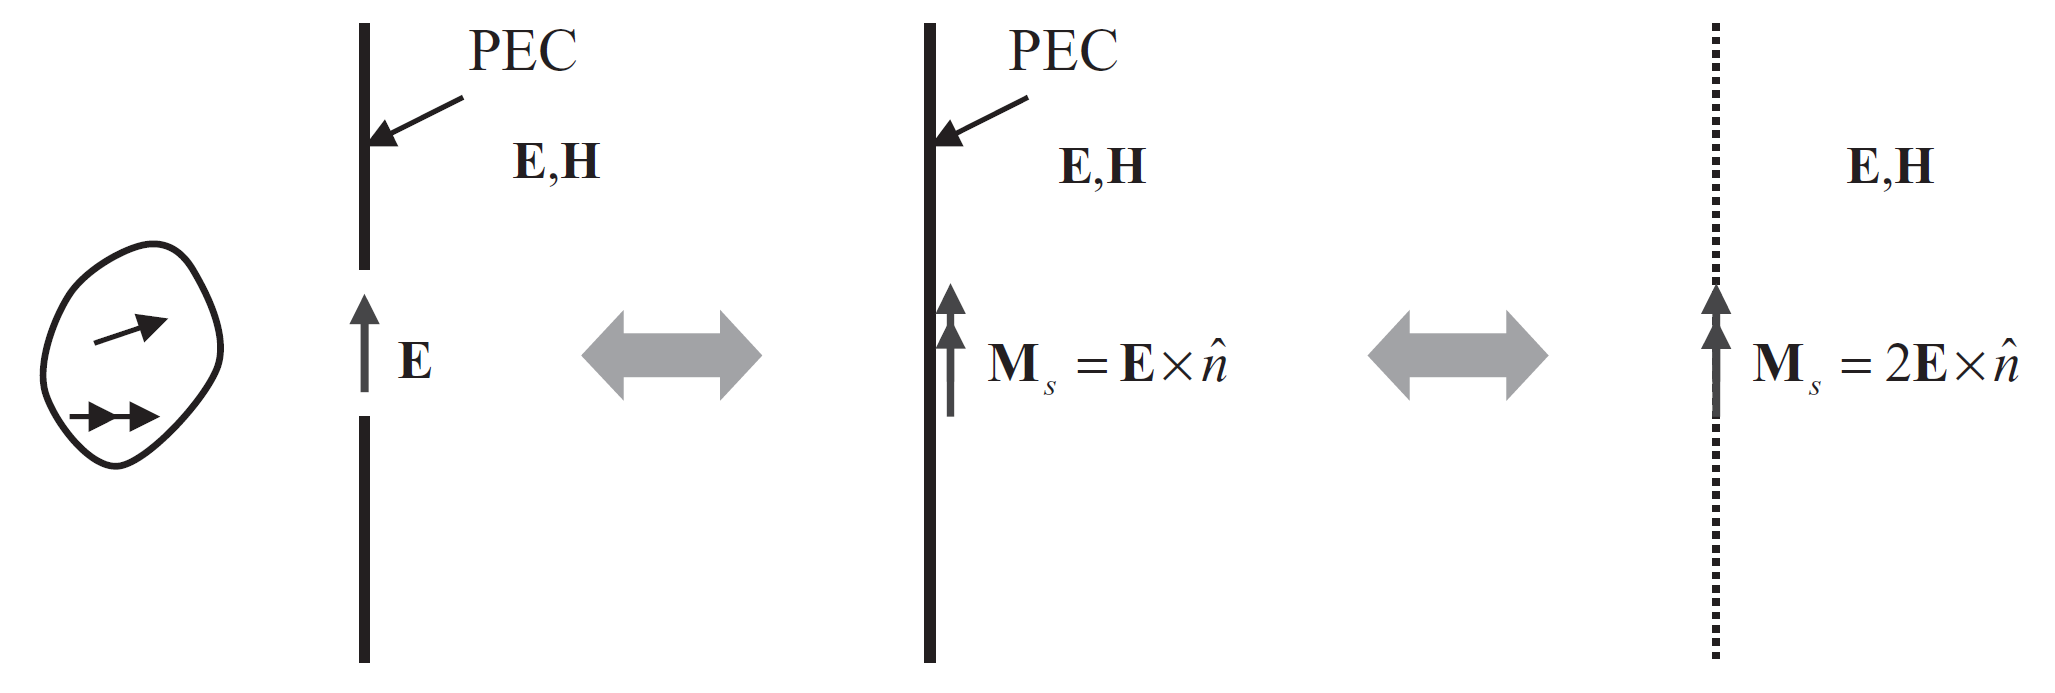
\includegraphics[width=0.5\textwidth]{穿过导体面口径的辐射.PNG}
    \caption{穿过导体面口径的辐射}
    \label{fig:fig25}
\end{figure}
\par
考虑位于$xy$平面的无限大导体平面上矩形波导开口的辐射,如图\ref{fig:fig26}所示。
\begin{figure}[ht]
    \centering
    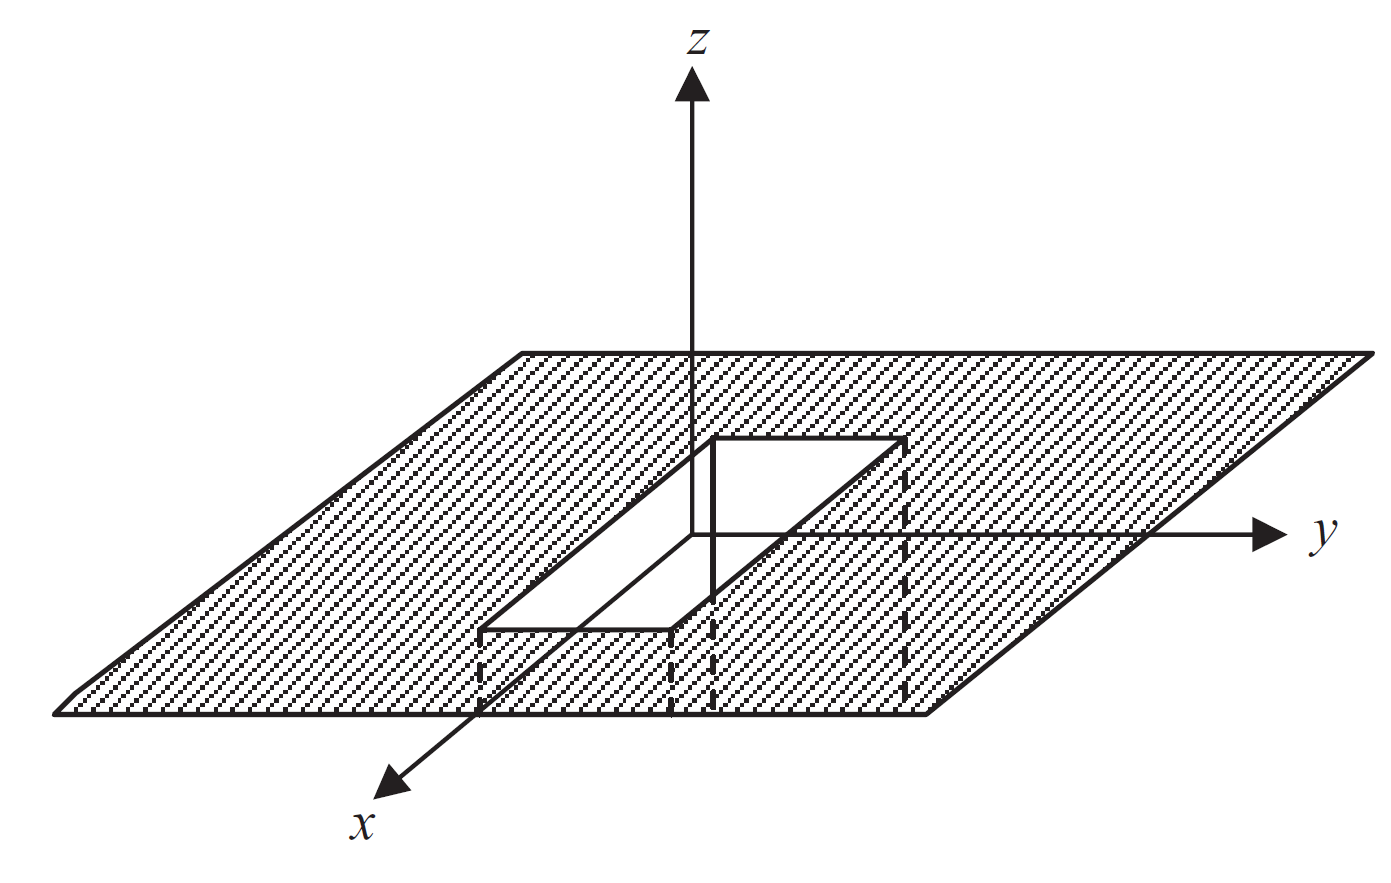
\includegraphics[width=0.5\textwidth]{无限大导体面上的矩形波导开口.PNG}
    \caption{无限大导体面上的矩形波导开口}
    \label{fig:fig26}
\end{figure}
\\
假设开口处电场为
\begin{align}
    \label{eq:eq251}
    \mathbf{E}=\hat{y}E_0\cos\frac{\pi s}{a}
\end{align}
则上半空间中的场可以等效为面磁流
\begin{align}
    \label{eq:eq252}
    \mathbf{M}_S=2\mathbf{E}\times\hat{z}=2\hat{x}E_0\cos\frac{\pi x}{a}
\end{align}
在自由空间中的辐射问题,若只关心远场,则只需要计算$\mathbf{L}$,根据式\ref{eq:eq118}
\begin{align}
    \label{eq:eq253}
    \mathbf{L}&=\iint_{S_a}\mathbf{M}_Se^{jkr'\cos\psi}dS'=\int_{-b/2}^{b/2}\int_{-a/2}^{a/2}2\hat{x}E_0\cos\frac{\pi x}{a}e^{jk(x'\sin\theta\cos\phi+y'\sin\theta\sin\phi)}dx'dy' \nonumber \\
              &=\hat{x}8\pi aE_0\frac{\cos\left(k\frac{a}{2}\sin\theta\cos\phi\right)\sin\left(k\frac{b}{2}\sin\theta\sin\phi\right)}{k[\pi^2-(ka\sin\theta\cos\phi)^2]\sin\theta\sin\phi}
\end{align}
根据式\ref{eq:eq119}以及式\ref{eq:eq123},对于$\theta\leq\pi/2$的远场,有
\begin{align}
    \label{eq:eq254}
    E_{\theta}&=\eta H_{\phi}=-\frac{jk}{4\pi r}e^{-jkr}L_{\phi} \nonumber \\
              &=j2aE_0\frac{e^{-jkr}}{r}\frac{\cos\left(k\frac{a}{2}\sin\theta\cos\phi\right)\sin\left(k\frac{b}{2}\sin\theta\sin\phi\right)}{[\pi^2-(ka\sin\theta\cos\phi)^2]\sin\theta} \\
    \label{eq:eq255}
    E_{\phi}&=-\eta H_{\theta}=\frac{jk}{4\pi r}e^{-jkr}L_{\theta} \nonumber \\
            &=j2aE_0\frac{e^{-jkr}}{r}\frac{\cos\left(k\frac{a}{2}\sin\theta\cos\phi\right)\sin\left(k\frac{b}{2}\sin\theta\sin\phi\right)}{[\pi^2-(ka\sin\theta\cos\phi)^2]\tan\theta\tan\phi}
\end{align}
其远场方向图如图\ref{fig:fig27}所示。
\begin{figure}[ht]
    \centering
    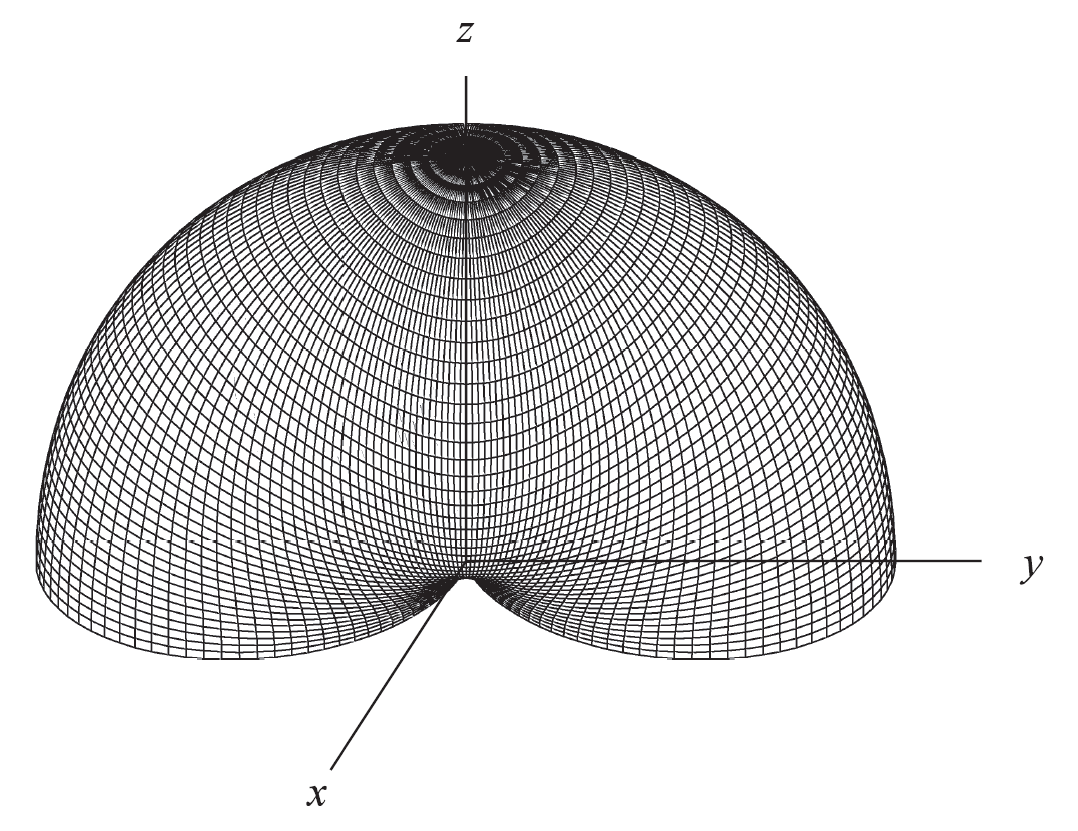
\includegraphics[width=0.5\textwidth]{无限大导体面上的矩形波导开口远场方向图.PNG}
    \caption{无限大导体面上的矩形波导开口远场方向图}
    \label{fig:fig27}
\end{figure}
\par
对于不存在无限大导体平面的情况,可以假想一个无限大平面,得到右半空间的场。参考图\ref{fig:fig28}所示的等效问题,将左半空间看作内区域,右半空间看作外区域,考虑三种等效方法。\\
(1)首先将左半空间看作零场,引入等效面电流$\mathbf{J}_S=\hat{n}\times\mathbf{H}$、等效面磁流$\mathbf{M}_S=\mathbf{E}\times\hat{n}$,则原问题等效为$\mathbf{J}_S$与$\mathbf{M}_S$在自由空间中的辐射问题。如图\ref{fig:fig29}所示。
\begin{figure}[ht]
    \centering
    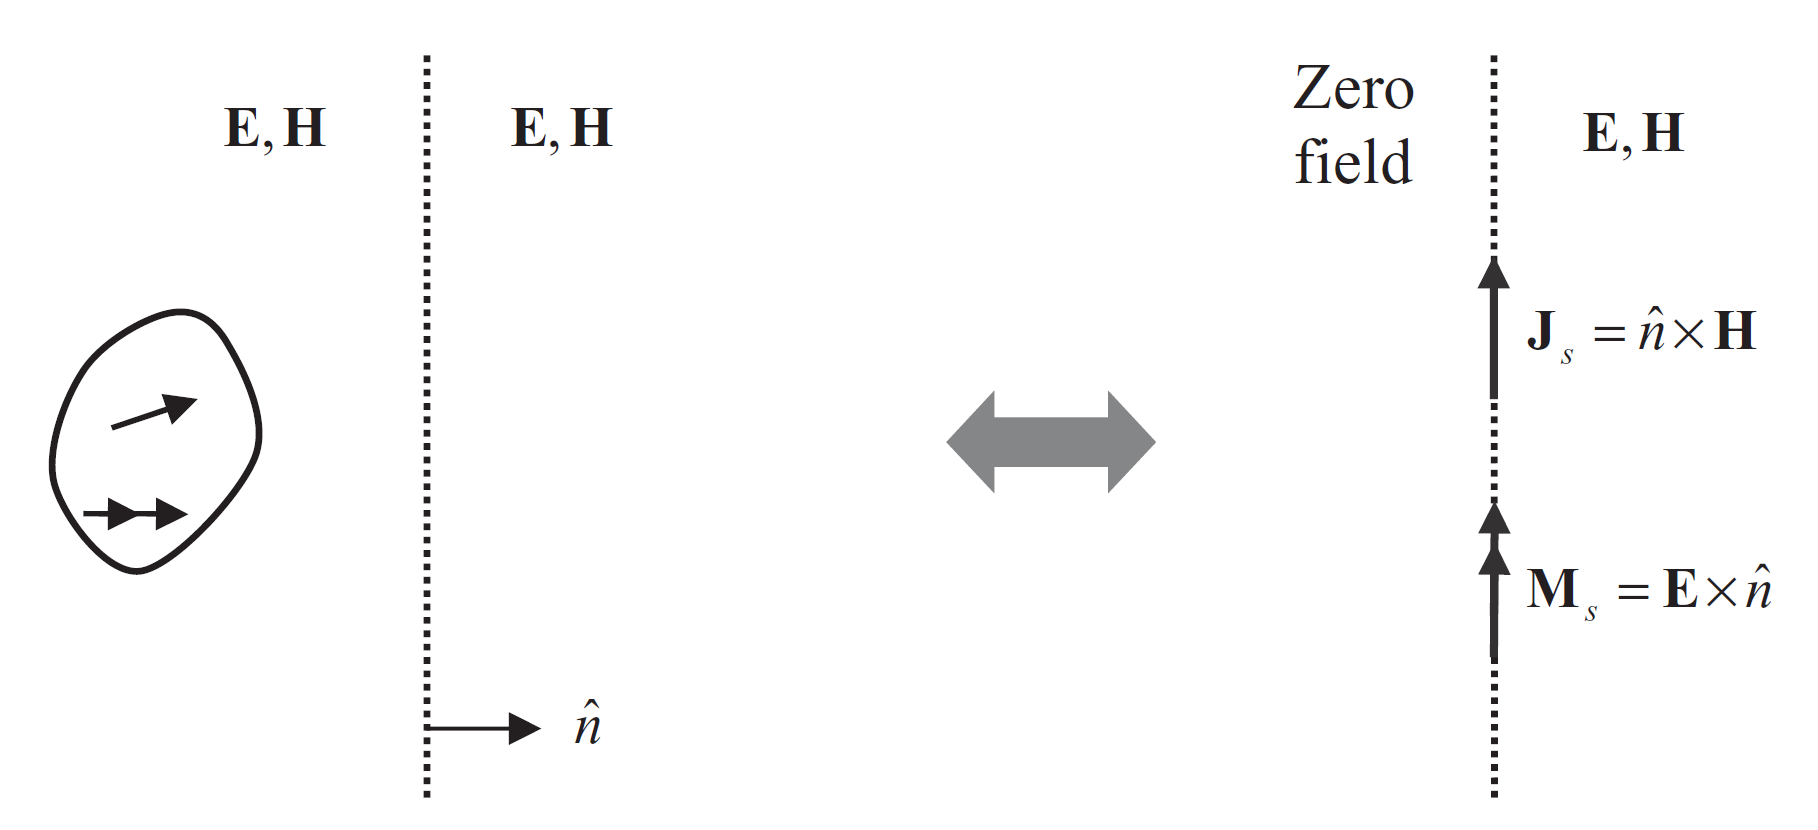
\includegraphics[width=0.5\textwidth]{通过一个虚拟平面向右半空间的辐射.PNG}
    \caption{通过一个虚拟平面向右半空间的辐射}
    \label{fig:fig29}
\end{figure}
\\
(2)在左半空间填充PEC,此时等效面电流不产生场,因此仅存在等效面磁流$\mathbf{M}_S=\mathbf{E}\times\hat{n}$。再利用镜像原理,将原问题转换为面磁流$\mathbf{M}_S=2\mathbf{E}\times\hat{n}$在自由空间的辐射问题。如图\ref{fig:fig30}所示。
\begin{figure}[ht]
    \centering
    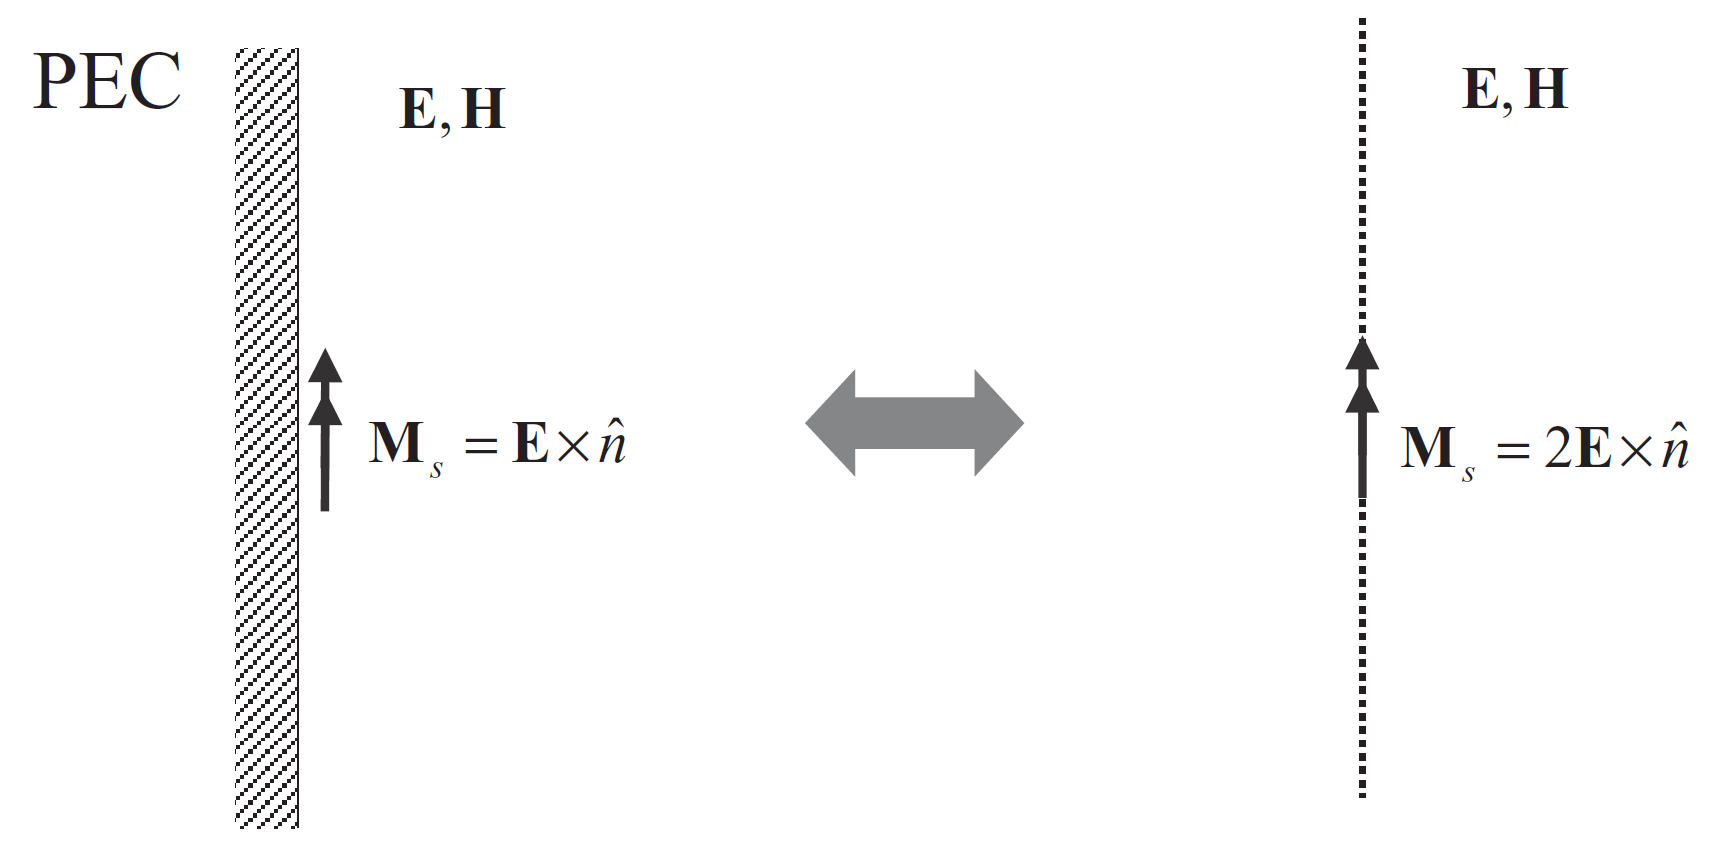
\includegraphics[width=0.5\textwidth]{通过填充PEC向右半空间的辐射.PNG}
    \caption{通过填充PEC向右半空间的辐射}
    \label{fig:fig30}
\end{figure}
\\
(3)在左半空间填充PMC,此时等效面磁流不产生场,因此仅存在等效面电流$\mathbf{J}_S=\hat{n}\times\mathbf{H}$。再利用镜像原理,将原问题转换为面磁流$\mathbf{J}_S=2\hat{n}\times\mathbf{H}$在自由空间的辐射问题。如图\ref{fig:fig31}所示。
\begin{figure}[ht]
    \centering
    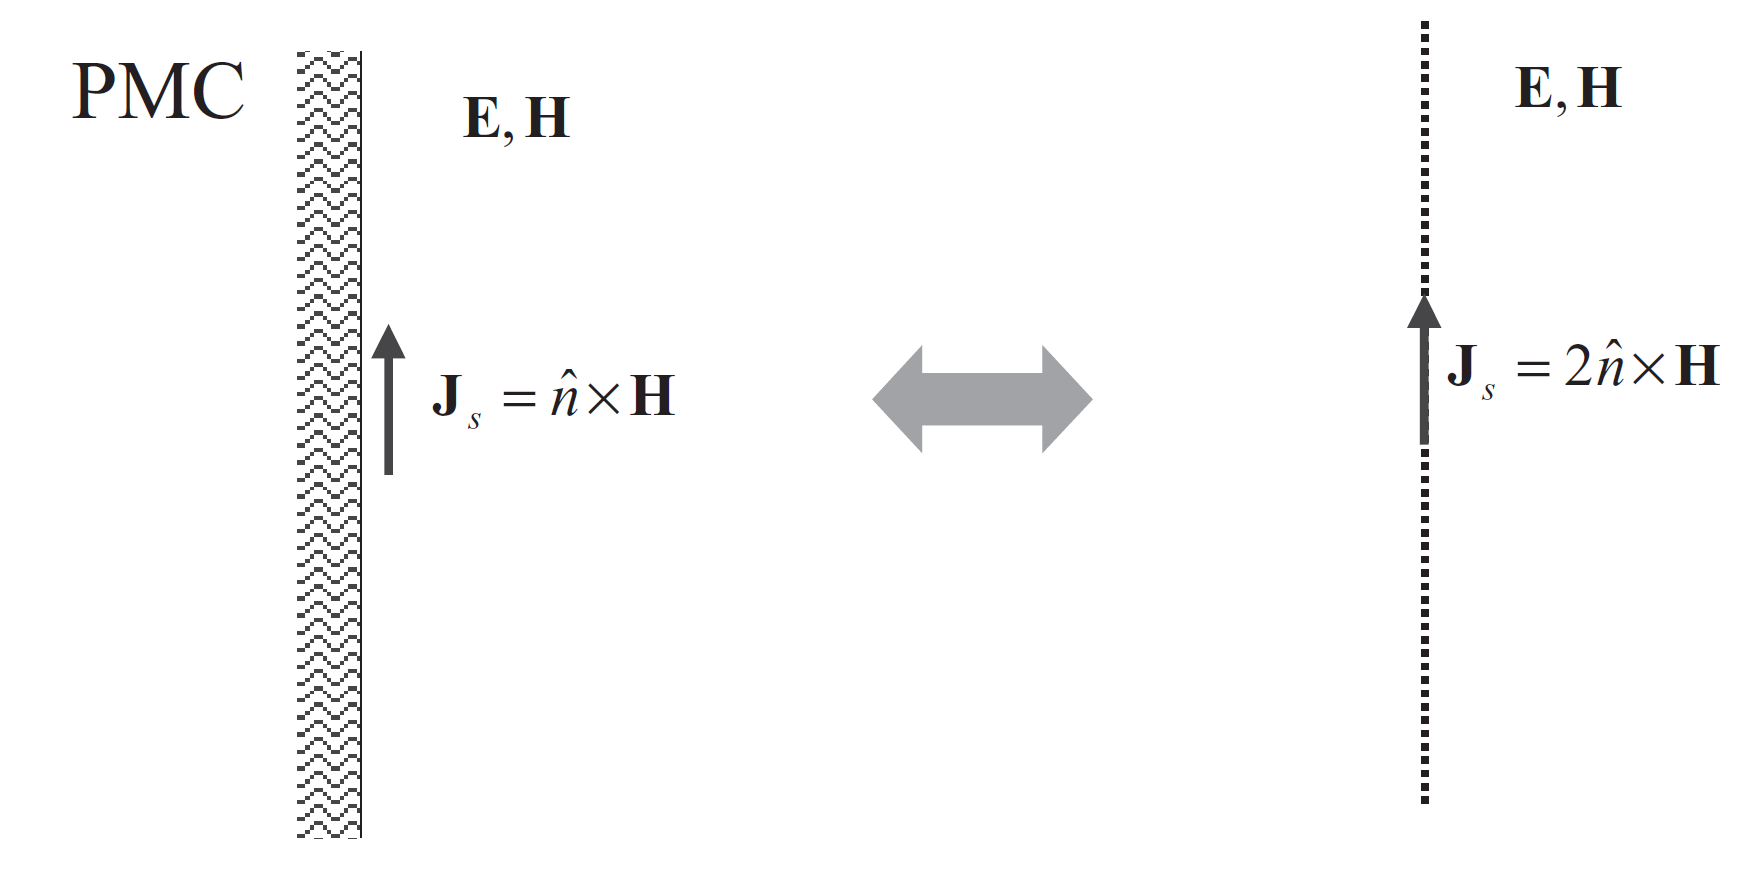
\includegraphics[width=0.5\textwidth]{通过填充PMC向右半空间的辐射.PNG}
    \caption{通过填充PMC向右半空间的辐射}
    \label{fig:fig31}
\end{figure}
\\如果切向场$\hat{n}\times\mathbf{H}$和$\hat{n}\times\mathbf{E}$在整个平面上准确已知,则三种等效问题得到相同的解,如果切向场式近似的,则三种等小问题得到的解略有差别。等效方法的选择依赖于特定问题给定的场信息。
\subsubsection{巴比涅原理}
通过考虑以下三个问题建立电磁场的巴比涅原理:\\
(1)电流源和磁流源$(\mathbf{J}_i,\mathbf{M}_i)$在自由空间中辐射,辐射场记为$(\mathbf{E}^{inc},\mathbf{H}^{inc})$,如图\ref{fig:fig32}所示。
\begin{figure}[ht]
    \centering
    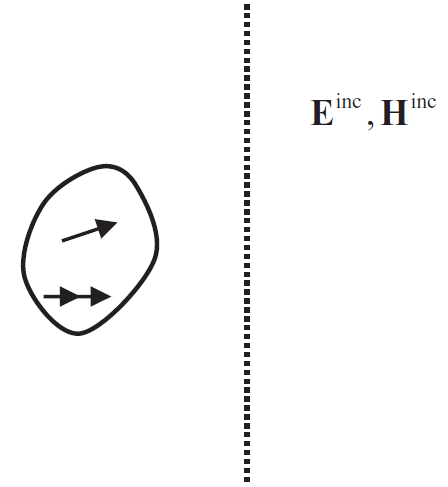
\includegraphics[width=0.25\textwidth]{向自由空间辐射的电磁源.PNG}
    \caption{向自由空间辐射的电磁源}
    \label{fig:fig32}
\end{figure}
\\
(2)电流源和磁流源$(\mathbf{J}_i,\mathbf{M}_i)$向开有口径的无限大PEC平面辐射,口径区域记为$S_a$,导体屏区域记为$S_m$,辐射场记为$(\mathbf{E}^{a},\mathbf{H}^{a})$,如图\ref{fig:fig33}所示。
\begin{figure}[ht]
    \centering
    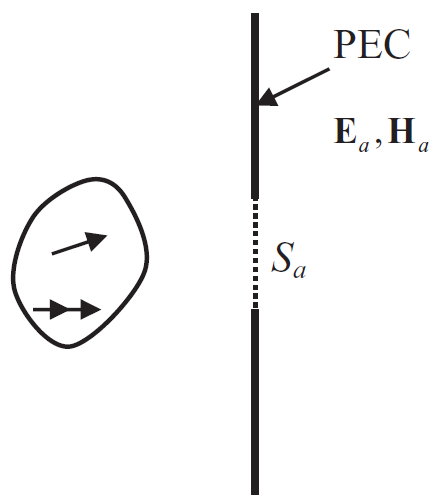
\includegraphics[width=0.25\textwidth]{向开有口径的无限大PEC平面辐射的电磁源.PNG}
    \caption{向开有口径的无限大PEC平面辐射的电磁源}
    \label{fig:fig33}
\end{figure}
\\
(3)电流源和磁流源$(\mathbf{J}_i,\mathbf{M}_i)$向有限大PMC平板辐射,PMC平板区域为$S_a$,其他区域为$S_m$,辐射场记为$(\mathbf{E}^{m},\mathbf{H}^{m})$,如图\ref{fig:fig34}所示。
\begin{figure}[ht]
    \centering
    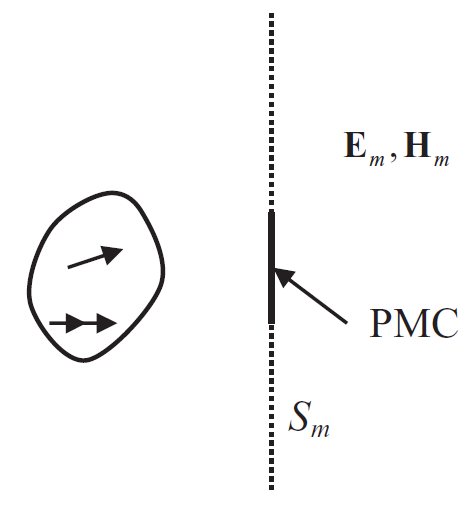
\includegraphics[width=0.25\textwidth]{向有限大PMC平板辐射的电磁源.PNG}
    \caption{向有限大PMC平板辐射的电磁源}
    \label{fig:fig34}
\end{figure}
\\
由式\ref{eq:eq127}知,电流源辐射磁场(仅有$\hat{\phi}$方向分量)的切向分量在任何包含电流源的平面上为零,所以在图\ref{fig:fig33}中,金属屏上的感应电流在口径上产生的磁场切向分量为零。因此,口径上的磁场切向分量等于原电流源和磁流源在自由空间产生的入射场的磁场切向分量,即
\begin{align}
    \label{eq:eq256}
    On~S_a:\qquad\hat{n}\times\mathbf{H}_a&=\hat{n}\times\mathbf{H}^{inc} \\
    \label{eq:eq257}
    On~S_m:\qquad\hat{n}\times\mathbf{E}_a&=0
\end{align}
由式\ref{eq:eq156}知,磁流源辐射电场(仅有$\hat{\phi}$方向分量)的切向分量在任何包含磁流源的平面上为零,所以在图\ref{fig:fig34}中,PMC板上的感应磁流在$S_m$区域产生的电场切向分量为零。因此,$S_m$区域的电场切向分量等于原电流源和磁流源在自由空间产生的入射场的电场切向分量,即
\begin{align}
    \label{eq:eq258}
    On~S_a:\qquad\hat{n}\times\mathbf{H}_m&=0 \\
    \label{eq:eq259}
    On~S_m:\qquad\hat{n}\times\mathbf{E}_m&=\hat{n}\times\mathbf{E}^{inc}
\end{align}
将图\ref{fig:fig33}和图\ref{fig:fig34}中的场相加,即
\begin{align}
    \label{eq:eq260}
    On~S_a:\qquad\hat{n}\times(\mathbf{H}_a+\mathbf{H}_m)&=\hat{n}\times\mathbf{H}^{inc} \\
    \label{eq:eq261}
    On~S_m:\qquad\hat{n}\times(\mathbf{E}_a+\mathbf{E}_m)&=\hat{n}\times\mathbf{E}^{inc}
\end{align}
根据唯一性定理,在右半空间中,叠加场与图\ref{fig:fig32}中的场相同,即
\begin{align}
    \label{eq:eq262}
    \mathbf{H}_a+\mathbf{H}_m&=\mathbf{H}^{inc} \\
    \label{eq:eq263}
    \mathbf{E}_a+\mathbf{E}_m&=\mathbf{E}^{inc}
\end{align}
以上即为\textbf{\color{blue}{巴比涅原理}}的电磁版本。也可将图\ref{fig:fig34}中的场写为
\begin{align}
    \label{eq:eq264}
    \mathbf{H}_m&=\mathbf{H}^{inc}+\mathbf{H}_m^{sc} \\
    \label{eq:eq265}
    \mathbf{E}_m&=\mathbf{E}^{inc}+\mathbf{E}_m^{sc}
\end{align}
其中,$(\mathbf{E}_m^{sc},\mathbf{H}_m^{sc})$是PMC平板上感应磁流产生的散射场。因此,巴比涅原理也可写成
\begin{align}
    \label{eq:eq266}
    \mathbf{H}_a&=-\mathbf{H}_m^{sc} \\
    \label{eq:eq267}
    \mathbf{E}_a&=-\mathbf{E}_m^{sc}
\end{align}
\par
根据对偶原理,将图\ref{fig:fig34}中的PMC平板换成PEC平板,求问题(3)的对偶问题,对偶源记为$(\mathbf{J}_d,\mathbf{M}_d)$,对偶场记为$(\mathbf{E}_d,\mathbf{H}_d)$,如图\ref{fig:fig35}所示。
\begin{figure}[ht]
    \centering
    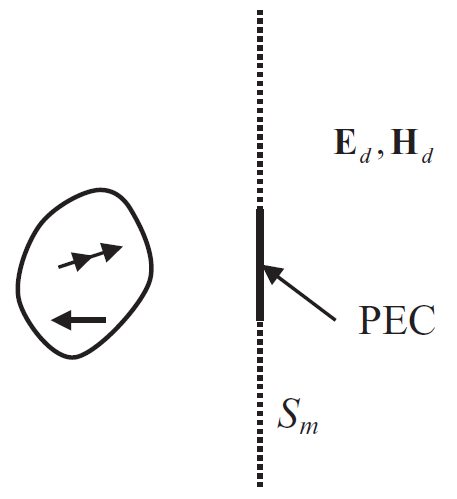
\includegraphics[width=0.25\textwidth]{对偶源向有限大PEC平板辐射的电磁源.PNG}
    \caption{对偶源向有限大PEC平板辐射的电磁源}
    \label{fig:fig35}
\end{figure}
\\
为了不再显现$\epsilon$和$\mu$,将表\ref{tab:tab1}中的对应关系变换成表\ref{tab:tab2}:
\begin{table}[!ht]
    \centering
    \caption{对偶公式的变换(不显现$\epsilon$和$\mu$)}
    \label{tab:tab2}
    \begin{tabular}{cc}
        \toprule
        原始公式 & 对偶公式 \\
        \midrule
        $\mathbf{E}$ & $\eta\mathbf{H}$ \\
        $\mathbf{H}$ & $-\frac{\mathbf{E}}{\eta}$ \\
        $\mathbf{J}$ & $\frac{\mathbf{M}}{\eta}$ \\
        $\mathbf{M}$ & $-\eta\mathbf{J}$ \\
        \bottomrule
     \end{tabular}
\end{table}
\\
由此,式\ref{eq:eq262}、式\ref{eq:eq263}写成
\begin{align}
    \label{eq:eq268}
    \mathbf{H}_a-\frac{\mathbf{E}_d}{\eta}&=\mathbf{H}^{inc} \\
    \label{eq:eq269}
    \mathbf{E}_a+\eta\mathbf{H}_d&=\mathbf{E}^{inc}
\end{align}
式\ref{eq:eq266}、式\ref{eq:eq267}写成
\begin{align}
    \label{eq:eq270}
    \mathbf{H}_a&=\frac{\mathbf{E}_d^{sc}}{\eta} \\
    \label{eq:eq271}
    \mathbf{E}_a&=-\eta\mathbf{H}_d^{sc}
\end{align}
\section{\textsf{传输线和平面波}}
\subsection{传输线理论}
\subsubsection{传输线方程及其解}
考虑有两根平行导体构成的传输线,其单位长度的电阻、电导、电感、电容分别为$R$、$G$、$L$、$C$,如图\ref{fig:fig36}表示长度为$\Delta z$的传输线的等效电路。
\begin{figure}[ht]
    \centering
    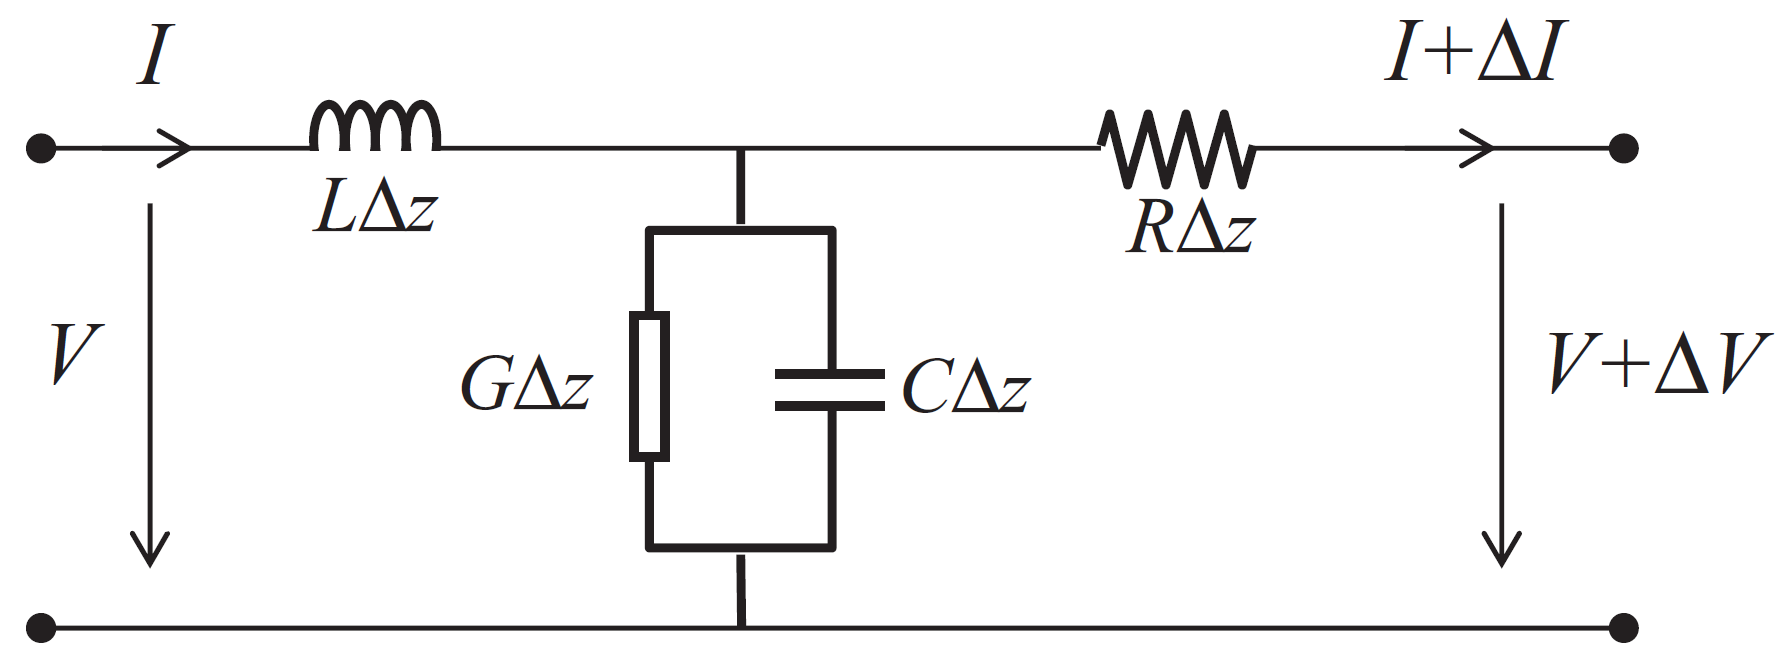
\includegraphics[width=0.5\textwidth]{一小段传输线的等效电路.PNG}
    \caption{一小段传输线的等效电路}
    \label{fig:fig36}
\end{figure}
\par
根据基尔霍夫电压和电流定律,有
\begin{align}
    \label{eq:eq272}
    jwL\Delta zI+R\Delta zI+\Delta V&=0 \\
    \label{eq:eq273}
    jwC\Delta zV+G\Delta zV+\Delta I&=0
\end{align}
当$\Delta z\to 0$时,有
\begin{align}
    \label{eq:eq274}
    \frac{dV}{dz}+(jwL+R)I&=0 \\
    \label{eq:eq275}
    \frac{dI}{dz}+(jwC+G)V&=0
\end{align}
消去$I$和$V$,得
\begin{align}
    \label{eq:eq276}
    \frac{d^2V}{dz^2}-\gamma^2V&=0 \\
    \label{eq:eq277}
    \frac{d^2I}{dz^2}-\gamma^2I&=0
\end{align}
式中,$\gamma^2=(jwL+R)(jwC+G)$,$\gamma$称为\textbf{\color{blue}{传播常数}}。
\par
接下来求解式\ref{eq:eq276}和式\ref{eq:eq277}由于他们具有相同的形式,因此只研究式\ref{eq:eq276}。其通解为
\begin{align}
    \label{eq:eq278}
    V(z)=a_+e^{-\gamma z}+a_-e^{\gamma z}
\end{align}
\par
对于考虑无耗传输线,即$R=G=0$,此时$\gamma^2=jw\sqrt{LC}=j\beta$,其中$\beta$为\textbf{\color{blue}{相位常数}}(rad/m),电压瞬时值为:
\begin{align}
    \label{eq:eq279}
    \mathcal{V}(z,t)&=Re\left[V(Z)e^{jwt}\right]=Re\left[a_+e^{j(wt-\beta z)}+a_-e^{j(wt+\beta z)}\right] \nonumber \\
                    &=|a_+|\cos(wt-\beta z+\angle a_+)+|a_-|\cos(wt+\beta z+\angle a_-)
\end{align}
式中,$|a_{\pm}|$和$\angle a_{\pm}$分别是$a_{\pm}$的幅度和相位。上式中,通过观察等相位点,第一项代表沿$+z$方向传播的波,第二项代表沿$-z$方向传播的波,其传播速度称为\textbf{\color{blue}{相速}}:
\begin{align}
    \label{eq:eq280}
    v_p=\frac{w}{\beta}=\frac{1}{\sqrt{LC}}
\end{align}
波长与相速的关系为$\lambda=v_p/f=2\pi v_p/w$,因此有$\beta=2\pi /\lambda$,所以相位常数也成为波数。\par
将式\ref{eq:eq278}代入式\ref{eq:eq274}中,得电流的频域表达式为:
\begin{align}
    \label{eq:eq281}
    I(z)=\sqrt{\frac{C}{L}}(a_+e^{-j\beta z}+a_-e^{j\beta z})
\end{align}
电流时域表达式为:
\begin{align}
    \label{eq:eq282}
    \mathcal{I}(z,t)=\sqrt{\frac{C}{L}}[|a_+|\cos(wt-\beta z+\angle a_+)+|a_-|\cos(wt+\beta z+\angle a_-)]
\end{align}
只考虑沿$+z$方向传播的波,其功率为:
\begin{align}
    \label{eq:eq283}
    \mathcal{P}_+(z,t)=\mathcal{I}_+(z,t)\mathcal{V}_+(z,t)=\sqrt{\frac{C}{L}}|a_+|^2\cos^2(wt-\beta z+\angle a_+)
\end{align}
单位长度传输线存储的电能与磁能分别为:
\begin{align}
    \label{eq:eq284}
    \mathcal{W}_{e+}(z,t)&=\frac{1}{2}C\mathcal{V}_+^2(z,t)=\frac{1}{2}C|a_+|^2\cos^2(wt-\beta z+\angle a_+) \\
    \label{eq:eq285}
    \mathcal{W}_{m+}(z,t)&=\frac{1}{2}L\mathcal{I}_+^2(z,t)=\frac{1}{2}C|a_+|^2\cos^2(wt-\beta z+\angle a_+)
\end{align}
定义能量传播的速度为\textbf{\color{blue}{能速}}:
\begin{align}
    \label{eq:eq286}
    v_e=\frac{\mathcal{P}_+(z,t)}{\mathcal{W}_{e+}(z,t)\mathcal{W}_{m+}(z,t)}=\frac{1}{\sqrt{LC}}
\end{align}
与相速相同。定义无耗传输线的\textbf{\color{blue}{特征阻抗}}:
\begin{align}
    \label{eq:eq287}
    Z_0=\frac{V_+}{I_+}=\sqrt{\frac{L}{C}}
\end{align}
只与传输线本身性质有关。\par
对于有耗传输线,
\begin{align}
    \label{eq:eq288}
    \gamma=\pm\sqrt{(jwL+R)(jwC+G)}=\pm\alpha\pm j\beta
\end{align}
其中
\begin{align}
    \label{eq:eq289}
    \alpha&=\sqrt{\frac{w^2LC-RG}{2}}\sqrt{\sqrt{1+\frac{w^2(GL+RC)^2}{(w^2LC-RG)^2}}-1} \\
    \label{eq:eq290}
    \beta&=\sqrt{\frac{w^2LC-RG}{2}}\sqrt{\sqrt{1+\frac{w^2(GL+RC)^2}{(w^2LC-RG)^2}}+1}
\end{align}
式\ref{eq:eq288}的四个解中,唯一有物理意义的解是$\gamma=\alpha+j\beta$,此时,电压的瞬时值为:
\begin{align}
    \label{eq:eq291}
    \mathcal{V}(z,t)&=Re\left[V(Z)e^{jwt}\right]=Re\left[a_+e^{j(wt-\beta z)-\alpha z}+a_-e^{j(wt+\beta z)+\alpha z}\right] \nonumber \\
                    &=|a_+|e^{-\alpha z}\cos(wt-\beta z+\angle a_+)+|a_-|e^{\alpha z}\cos(wt+\beta z+\angle a_-)
\end{align}
上式中,第一项代表沿$+z$方向传播的波,其以$e^{-\alpha z}$的规律衰减,第二项代表沿$-z$方向传播的波,以同样的规律衰减。$\alpha$称为\textbf{\color{blue}{衰减常数}}(Np/m)。\par
将式\ref{eq:eq278}代入式\ref{eq:eq274}中,得电流的频域表达式为:
\begin{align}
    \label{eq:eq292}
    I(z)=\frac{\gamma}{jwL+R}\left[a_+e^{-(\alpha+j\beta) z}+a_-e^{(\alpha+j\beta) z}\right]
\end{align}
特征阻抗为:
\begin{align}
    \label{eq:eq293}
    Z_0=\frac{V_+}{I_+}=\frac{jwL+R}{\gamma}=\sqrt{\frac{jwL+R}{jwC+G}}
\end{align}
\subsubsection{反射和透射}
考虑在$z=0$处相接的两段特征阻抗不同的半无限长传输线,$z<0$区域的特征阻抗为$Z_{01}$,$z>0$区域的特征阻抗为$Z_{02}$,一个波从$z<0$区域沿$+z$方向传播,当其到达$z=0$处时,一部分功率反射回来,另一部分功率继续沿$+z$方向传播,如图\ref{fig:fig37}所示。
\begin{figure}[ht]
    \centering
    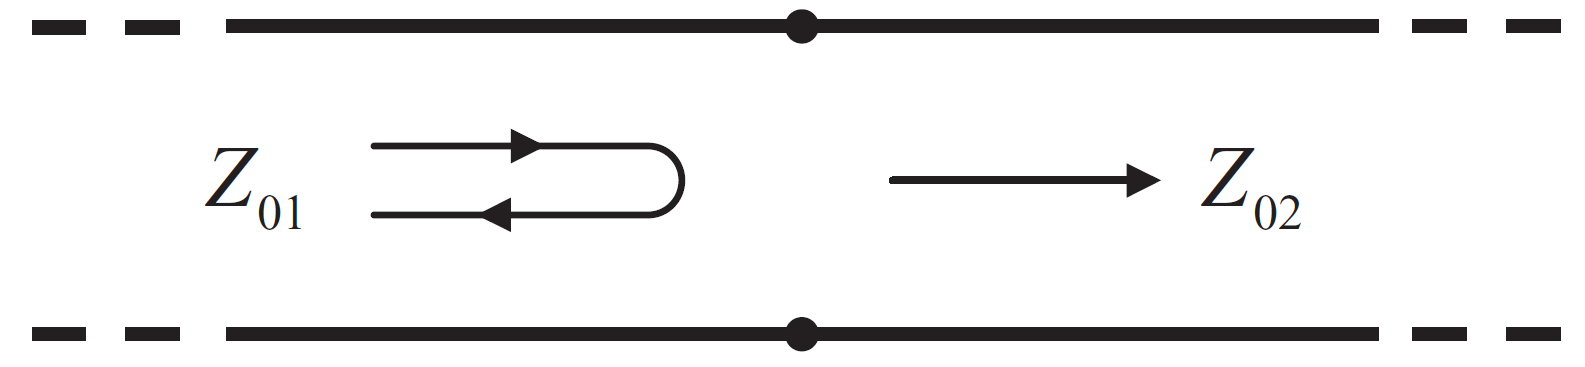
\includegraphics[width=0.4\textwidth]{两段半无限长传输线连接处的反射和透射.PNG}
    \caption{两段半无限长传输线连接处的反射和透射}
    \label{fig:fig37}
\end{figure}
传输线上的总电压为:
\begin{align}
    \label{eq:eq294}
    V(z)=
    \left\{
        \begin{array}{lr}
            a_+e^{-\gamma z}+\Gamma a_+e^{\gamma z}, &z<0 \\
            Ta_+e^{-\gamma z},                       &z>0
        \end{array}
    \right.
\end{align}
式中,$a_+$表示入射波幅度,$\Gamma$为反射系数,$T$为透射系数。相应的电流为:
\begin{align}
    \label{eq:eq295}
    I(z)=
    \left\{
        \begin{array}{lr}
            (a_+e^{-\gamma z}+\Gamma a_+e^{\gamma z})/Z_{01}, &z<0 \\
            Ta_+e^{-\gamma z}/Z_{02},                         &z>0
        \end{array}
    \right.
\end{align}
在$z=0$处,电压和电流连续,因此有
\begin{align}
    \label{eq:eq296}
    \Gamma&=\frac{Z_{02}-Z_{01}}{Z_{02}+Z_{01}} \\
    \label{eq:eq297}
    T&=\frac{2Z_{02}}{Z_{02}+Z_{01}}
\end{align}
\par
考虑在$z=z_0$的终端连接阻抗负载$Z_L$的均匀传输线,传输线阻抗为$Z_0$,则仅存在反射,不存在透射,如图\ref{fig:fig38}所示。
\begin{figure}[ht]
    \centering
    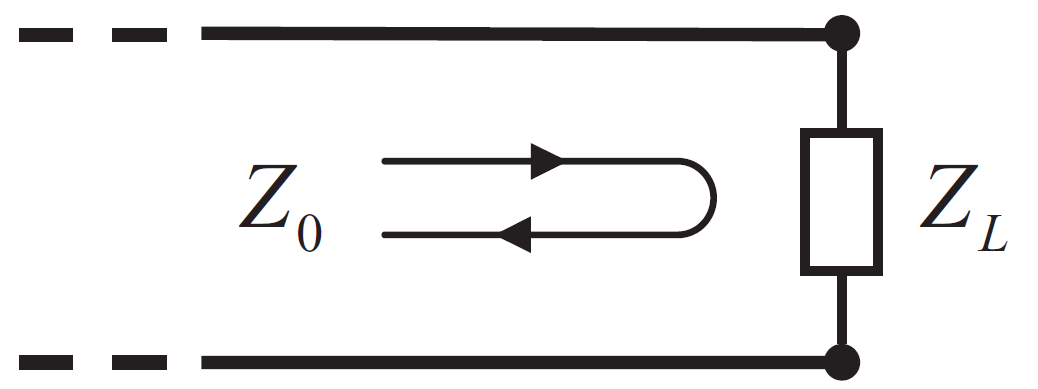
\includegraphics[width=0.3\textwidth]{传输线上的阻抗负载引起的反射.PNG}
    \caption{传输线上的阻抗负载引起的反射}
    \label{fig:fig38}
\end{figure}
则传输线上的总电压、总电流为:
\begin{align}
    \label{eq:eq298}
    V(z)&=a_+e^{-\gamma z}+\Gamma a_+e^{\gamma z} \\
    \label{eq:eq299}
    I(z)&=\frac{1}{Z_0}(a_+e^{-\gamma z}-\Gamma a_+e^{\gamma z})
\end{align}
在$z=z_0$处,电压和电流满足$V(z_0)/I(z_0)=Z_L$,因此有
\begin{align}
    \label{eq:eq300}
    \Gamma&=\frac{Z_{L}-Z_{0}}{Z_{L}+Z_{0}}e^{-2\gamma z_0}
\end{align}
定义$z$处的阻抗为:
\begin{align}
    \label{eq:eq301}
    Z(z)=\frac{V(z)}{I(z)}=Z_0\frac{1+\Gamma e^{2\gamma z}}{1-\Gamma e^{2\gamma z}}=Z_0\frac{1+\Gamma(z)}{1-\Gamma(z)}=Z_0\frac{Z_L\cosh\gamma l+Z_0\sinh\gamma l}{Z_0\cosh\gamma l+Z_L\sinh\gamma l}
\end{align}
式中,$\Gamma(z)=\Gamma e^{2\gamma z}$表示$z$处的反射系数,$l=z_0-z$。当传输线无耗时,
\begin{align}
    \label{eq:eq302}
    Z(z)=Z_0\frac{Z_L\cos\beta l+Z_0\sin\beta l}{Z_0\cos\beta l+Z_L\sin\beta l}
\end{align}
因此,阻抗值与观察点位置和终端负载有关:\\
(1)当$Z_L=Z_0$(匹配)时,$\Gamma=0$,$Z(z)=Z_0$; \\
(2)当$Z_L=0$(短路)时,$\Gamma(z_0)=-1$,$Z(z)=jZ_0\tan\beta l$; \\
(3)当$Z_L=\infty$(开路)时,$\Gamma(z_0)=1$,$Z(z)=-jZ_0\tan\beta l$。 \\
当$\beta l=\pi/2$即$l=\lambda/4$时,短路变开路,开路变短路。
\subsubsection{格林函数}
考虑一段由分布电流源$i(z)$激励的传输线,如图\ref{fig:fig39}所示。
\begin{figure}[ht]
    \centering
    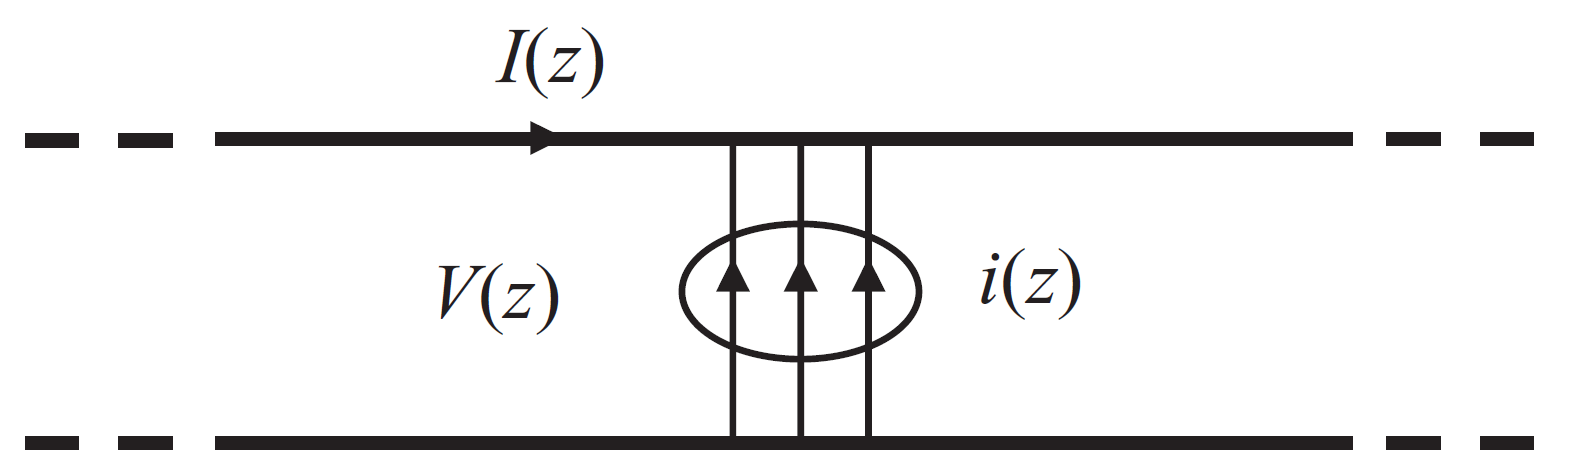
\includegraphics[width=0.5\textwidth]{由分布电流源激励的传输线.PNG}
    \caption{由分布电流源激励的传输线}
    \label{fig:fig39}
\end{figure}
则根据基尔霍夫电压和电流定律,有
\begin{align}
    \label{eq:eq303}
    \frac{dV}{dz}+(jwL+R)I&=0 \\
    \label{eq:eq304}
    \frac{dI}{dz}+(jwC+G)V&=i(z)
\end{align}
则电压满足二阶微分方程:
\begin{align}
    \label{eq:eq305}
    \frac{d^2V}{dz^2}-\gamma^2V=-(jwL+R)i(z)
\end{align}
上式为线性方程,因此,用线性叠加的方式表示该方程的解:
\begin{align}
    \label{eq:eq306}
    V(z)=(jwL+R)\int^{z_2}_{z_1}g(z,z')i(z')dz'
\end{align}
式中,$i(z)$存在的范围是$[z_1,z_2]$,$g(z,z')$称为\textbf{\color{blue}{格林函数}},将电流写成线性叠加的形式:
\begin{align}
    \label{eq:eq307}
    i(z)=\int^{z_2}_{z_1}\delta(z-z')i(z')dz'
\end{align}
将式\ref{eq:eq306}、式\ref{eq:eq307}代入式\ref{eq:eq305},得关于$g(z,z')$的二阶微分方程:
\begin{align}
    \label{eq:eq308}
    \frac{d^2g(z,z')}{dz^2}-\gamma^2g(z,z')=-\delta(z-z')
\end{align}
则对于无限长传输线,上述方程的解为:
\begin{align}
    \label{eq:eq309}
    g_0(z,z')=
    \left\{
        \begin{array}{lr}
            Ae^{\gamma z}, &z<z' \\
            Be^{-\gamma z}, &z>z'
        \end{array}
    \right.
\end{align}
对于有限长传输线,需要在解中加入代表反射波的项。由于没有电压源,所以电压连续,因此$g_0(z,z')$也连续,即
\begin{align}
    \label{eq:eq310}
    g_0(z,z')|_{z=z'+0}=g_0(z,z')|_{z=z'-0}
\end{align}
对式\ref{eq:eq308}在包含$z'$的一个小区间内积分,可得
\begin{align}
    \label{eq:eq311}
    \left.\frac{dg_0(z,z')}{dz}\right|_{z=z'+0}-\left.\frac{dg_0(z,z')}{dz}\right|_{z=z'-0}=-1
\end{align}
将式\ref{eq:eq309}分别代入式\ref{eq:eq310}、式\ref{eq:eq311},确定未知数$A$、$B$,得到
\begin{align}
    \label{eq:eq312}
    g_0(z,z')=\frac{1}{2\gamma}
    \left\{
        \begin{array}{lr}
            e^{\gamma z}, &z\leq z' \\
            e^{-\gamma z}, &z\geq z'
        \end{array}
    \right.
\end{align}
\subsubsection{特征函数展开}
考虑另一种方法求解方程\ref{eq:eq308}。用傅里叶变换将$g_0(z,z')$、$\delta(z-z')$展开为:
\begin{align}
    \label{eq:eq313}
    g_0(z,z')&=\frac{1}{2\pi}\int^{\infty}_{-\infty}f(h)e^{jhz}dh \\
    \label{eq:eq314}
    \delta(z-z')&=\frac{1}{2\pi}\int^{\infty}_{-\infty}e^{jh(z-z')}dh
\end{align}
代入方程\ref{eq:eq308},可得
\begin{align}
    \label{eq:eq315}
    f(h)=\frac{e^{-jhz'}}{h^2+\gamma^2}
\end{align}
则
\begin{align}
    \label{eq:eq316}
    g_0(z,z')&=\frac{1}{2\pi}\int^{\infty}_{-\infty}\frac{e^{jh(z-z')}}{h^2+\gamma^2}dh=\frac{1}{2\gamma}
    \left\{
        \begin{array}{lr}
            e^{\gamma z}, &z\leq z' \\
            e^{-\gamma z}, &z\geq z'
        \end{array}
    \right.
\end{align}
上式的积分通过\textbf{\color{blue}{柯西留数定理}}计算\footnote{被积函数有两个极点:$h=\pm j\gamma$,为保证结果有物理意义,对于$z-z'<0$,环路积分在下半平面进行,对于$z-z'>0$,环路积分在下半平面进行。},得到结果与上节结果一致,这种方法称为\textbf{\color{blue}{特征函数展开法}},即将$g_0(z,z')$按特征函数$e^{jhz}$展开,特征值为$h$,这些特征函数式齐次方程
\begin{align}
    \label{eq:eq317}
    \frac{d^2f}{dz^2}-h^2f=0
\end{align}
的解。特征函数展开法更具有系统性,能推广到更一般的问题中,方程\ref{eq:eq90}也可以使用这种方法求解。
\subsection{波动方程}
\subsubsection{波动方程及其通解}
考虑无源媒质中的麦克斯韦方程:
\begin{align}
    \label{eq:eq318}
    \nabla \times \mathbf{E}&=-jw\mu\mathbf{H} \\
    \label{eq:eq319}
    \nabla \times \mathbf{H}&=jw\epsilon\mathbf{E}+\sigma\mathbf{E}
\end{align}
从而得到电场和磁场满足的矢量亥姆霍兹方程:
\begin{align}
    \label{eq:eq320}
    \nabla^2\mathbf{E}-\gamma^2\mathbf{E}&=0 \\
    \label{eq:eq321}
    \nabla^2\mathbf{H}-\gamma^2\mathbf{H}&=0
\end{align}
式中$\gamma^2=jw\mu(jw\epsilon+\sigma)$。电场和磁场在笛卡尔坐标系中的每一个分量都满足标量亥姆霍兹方程,因此有
\begin{align}
    \label{eq:eq322}
    \nabla^2{E}_x-\gamma^2{E}_x=\frac{\partial^2E_x}{\partial x^2}+\frac{\partial^2E_x}{\partial y^2}+\frac{\partial^2E_x}{\partial z^2}-\gamma^2{E}_x=0
\end{align}
假设$E_x=X(x)Y(y)Z(z)$,则有
\begin{align}
    \label{eq:eq323}
    \frac{1}{X}\frac{\partial^2X}{\partial x^2}+\frac{1}{Y}\frac{\partial^2Y}{\partial y^2}+\frac{1}{Z}\frac{\partial^2Z}{\partial z^2}-\gamma^2=0
\end{align}
上式中的前三项相互独立,要使其成立,前三项必须是常数,故
\begin{align}
    \label{eq:eq324}
    \frac{1}{X}\frac{\partial^2X}{\partial x^2}=\gamma_x^2 \\
    \label{eq:eq325}
    \frac{1}{Y}\frac{\partial^2Y}{\partial y^2}=\gamma_y^2 \\
    \label{eq:eq326}
    \frac{1}{Z}\frac{\partial^2Z}{\partial z^2}=\gamma_z^2
\end{align}
其解分别为
\begin{align}
    \label{eq:eq327}
    X=A_xe^{\pm\gamma_xx} \\
    \label{eq:eq328}
    Y=A_xe^{\pm\gamma_yy} \\
    \label{eq:eq329}
    Z=A_xe^{\pm\gamma_zz}
\end{align}
因此,$E_x$的解为:
\begin{align}
    \label{eq:eq330}
    E_x=Ae^{\pm\gamma_xx\pm\gamma_yy\pm\gamma_zz}
\end{align}
式中$A=A_xA_yA_z$。$E_y$和$E_z$同样满足类似的解,因此,矢量场$\mathbf{E}$的解为:
\begin{align}
    \label{eq:eq331}
    \mathbf{E}(x,y,z)=\mathbf{E}(\vec{r})=\mathbf{E}_0e^{\pm\gamma_xx\pm\gamma_yy\pm\gamma_zz}=\mathbf{E}_0e^{\pm\vec{\gamma}\cdot\vec{r}}
\end{align}
式中,$\mathbf{E}_0$为任意常矢量,$\vec{\gamma}=\hat{x}\gamma_x+\hat{y}\gamma_y+\hat{z}\gamma_z$,$\vec{r}=\hat{x}x+\hat{y}y+\hat{z}z$,其中$\gamma_x^2+\gamma_y^2+\gamma_z^2=\gamma^2$。类似的,矢量场$\mathbf{H}$的解为:
\begin{align}
    \label{eq:eq332}
    \mathbf{H}(\vec{r})=\mathbf{H}_0e^{\pm\vec{\gamma}\cdot\vec{r}}
\end{align}
令$\vec{\gamma}=\vec{\alpha}+j\vec{\beta}$,则电场的瞬时值为
\begin{align}
    \label{eq:eq333}
    \mathcal{\vec{E}}(\vec{r},t)=Re\left[\mathbf{E}_0e^{jwt\pm(\vec{\alpha}+j\vec{\beta})\cdot\vec{r}}\right]=\mathbf{E}_0e^{\pm\vec{\alpha}\cdot\vec{r}}\cos(wt\pm\vec{\beta}\cdot\vec{r})
\end{align}
假设$\mathbf{E}_0$是实矢量,则$\cos(wt\pm\vec{\beta}\cdot\vec{r})$代表沿$\mp\hat{\beta}$方向传播的波,在$\vec{\beta}\cdot\vec{r}$为常数的平面上,相位相等,在$\vec{\alpha}\cdot\vec{r}$为常数的平面上,波的幅度均匀,因此,当$\vec{\alpha}$和$\vec{\beta}$方向相同时,等相面和等幅面相互平行,这样的波称为\textbf{\color{blue}{均匀平面波}},如果$\vec{\alpha}$和$\vec{\beta}$方向不相同,则称为\textbf{\color{blue}{非均匀平面波}}。
\subsubsection{平面波}
分别将式\ref{eq:eq331}、式\ref{eq:eq332}代入式\ref{eq:eq318}、式\ref{eq:eq319},得
\begin{align}
    \label{eq:eq334}
    \pm\vec{\gamma} \times \mathbf{E}&=-jw\mu\mathbf{H} \\
    \label{eq:eq335}
    \pm\vec{\gamma} \times \mathbf{H}&=(jw\epsilon+\sigma)\mathbf{E}
\end{align}
则$\vec{\gamma}$、$\mathbf{E}$、$\mathbf{H}$相互垂直。定义\textbf{\color{blue}{波阻抗}}为电场与磁场的比值:
\begin{align}
    \label{eq:eq336}
    Z_w=\frac{|\mathbf{E}|}{|\mathbf{H}|}=\sqrt{\frac{jw\mu}{jw\epsilon+\sigma}}
\end{align}
其与媒质的\textbf{\color{blue}{本征阻抗$\eta$}}相同,媒质的本征阻抗只和媒质本身特性有关,而波阻抗与电磁波类型相关,对于均匀平面波,二者相等,否则二者可能不相等。根据式\ref{eq:eq334}得
\begin{align}
    \label{eq:eq337}
    \vec{\gamma}\times(\vec{\gamma}\times\mathbf{E})=(\vec{\gamma}\cdot\mathbf{E})\vec{\gamma}-(\vec{\gamma}\cdot\vec{\gamma})\mathbf{E}=-(\vec{\gamma}\cdot\vec{\gamma})\mathbf{E}=-jw\mu(jw\epsilon+\sigma)\mathbf{E}
\end{align}
因为$\mathbf{E}\neq 0$,故
\begin{align}
    \label{eq:eq338}
    \vec{\gamma}\cdot\vec{\gamma}=\gamma_x^2+\gamma_y^2+\gamma_z^2=\gamma^2=jw\mu(jw\epsilon+\sigma)
\end{align}
上式称为\textbf{\color{blue}{色散关系}},建立了传播常数与媒质特性之间的联系。
\par
对于传播方向为$\hat{\beta}$且在无耗介质中的波,$\vec{\gamma}=j\vec{\beta}$\footnote{无耗媒质中,$\beta=w\sqrt{\mu\epsilon}$。},则式\ref{eq:eq334}、式\ref{eq:eq335}重写为
\begin{align}
    \label{eq:eq339}
    \vec{\beta} \times \mathbf{E}&=w\mu\mathbf{H} \\
    \label{eq:eq340}
    \vec{\beta} \times \mathbf{H}&=-w\epsilon\mathbf{E}
\end{align}
此时波阻抗为
\begin{align}
    \label{eq:eq341}
    Z_w=\frac{|\mathbf{E}|}{|\mathbf{H}|}=\sqrt{\frac{\mu}{\epsilon}}
\end{align}
色散关系为
\begin{align}
    \label{eq:eq342}
    \beta^2=w^2\mu\epsilon
\end{align}
$\beta$称为相位常数或波数。\par
考虑沿$\vec{r}=\hat{\beta}r$传播的均匀平面波,电场瞬时值式\ref{eq:eq333}写成
\begin{align}
    \label{eq:eq343}
    \mathcal{\vec{E}}(\vec{r},t)=\mathbf{E}_0\cos(wt-\vec{\beta}\cdot\vec{r})=\mathbf{E}_0\cos(wt-\beta r)
\end{align}
则相速为
\begin{align}
    \label{eq:eq344}
    v_p=\frac{w}{\beta}
\end{align}
表示等相面的移动速度。磁场的瞬时值为
\begin{align}
    \label{eq:eq345}
    \mathcal{\vec{H}}(\vec{r},t)=\mathbf{H}_0\cos(wt-\vec{\beta}\cdot\vec{r})=\frac{\hat{\beta}\times\mathbf{E}_0}{\eta}\cos(wt-\vec{\beta}\cdot\vec{r})
\end{align}
则能流密度的瞬时值为
\begin{align}
    \label{eq:eq346}
    \mathcal{\vec{S}}=\mathcal{\vec{E}}\times\mathcal{\vec{H}}=\hat{\beta}\frac{|\mathbf{E}_0|^2}{\eta}\cos^2(wt-\vec{\beta}\cdot\vec{r})
\end{align}
电能和磁能的瞬时值为
\begin{align}
    \label{eq:eq347}
    \mathcal{W}_e=\frac{1}{2}\epsilon\mathcal{\vec{E}}^2=\frac{1}{2}\epsilon|\mathbf{E}_0|^2\cos^2(wt-\vec{\beta}\cdot\vec{r}) \\
    \label{eq:eq348}
    \mathcal{W}_m=\frac{1}{2}\mu\mathcal{\vec{H}}^2=\frac{1}{2}\epsilon|\mathbf{E}_0|^2\cos^2(wt-\vec{\beta}\cdot\vec{r})
\end{align}
则无耗媒质中的能速为
\begin{align}
    \label{eq:eq349}
    v_e=\frac{power~flow~density}{energy~density}=\frac{\mathbf{S}}{\mathcal{W}_e+\mathcal{W}_m}=\frac{1}{\sqrt{\mu\epsilon}}
\end{align}
与相速相等(仅适用于均匀平面波)。\textbf{\color{blue}{群速}}是指包络的移动速度,其定义为
\begin{align}
    \label{eq:eq350}
    v_g=\lim_{\Delta w\to 0}\frac{\Delta w}{\Delta \beta}=\left(\frac{d\beta}{dw}\right)^{-1}
\end{align}
因此,在无耗非色散媒质中,群速为$v_g=\frac{1}{\sqrt{\mu\epsilon}}$。当$\epsilon$和$\mu$随频率变化时,有
\begin{align}
    \label{eq:eq351}
    v_g=\left(\frac{d\beta}{dw}\right)^{-1}=\left[\frac{d}{dw}\left(\frac{w}{v_p}\right)\right]^{-1}=\frac{v_p}{1-\frac{w}{v_p}\frac{dv_p}{dw}}
\end{align}
上式给出了群速和相速之间的关系。在非色散媒质中,$dv_p/dw=0$,故$v_g=v_p$;在正常色散媒质中,$dv_p/dw<0$,故$v_g<v_p$;在反色散媒质中,$dv_p/dw>0$,故$v_g>v_p$。\par
对于有耗介质,$\gamma=\alpha+j\beta=\sqrt{jw\mu(jw\epsilon+\sigma)}$,其中
\begin{align}
    \label{eq:eq352}
    \alpha=w\sqrt{\frac{\mu\epsilon}{2}}\sqrt{\sqrt{1+\left(\frac{\sigma}{w\epsilon}\right)^2}-1} \\
    \label{eq:eq353}
    \beta=w\sqrt{\frac{\mu\epsilon}{2}}\sqrt{\sqrt{1+\left(\frac{\sigma}{w\epsilon}\right)^2}+1}
\end{align}
对于良介质,$(\sigma/w\epsilon)^2\ll 1$,
\begin{align}
    \label{eq:eq354}
    \alpha\approx\frac{\sigma}{2}\sqrt{\frac{\mu}{\epsilon}}\qquad\beta\approx w\sqrt{\mu\epsilon}\qquad\eta\approx\sqrt{\frac{\mu}{\epsilon}}
\end{align}
对于良导体,$(\sigma/w\epsilon)^2\gg 1$,
\begin{align}
    \label{eq:eq355}
    \alpha\approx\sqrt{\frac{w\mu\sigma}{2}}\qquad\beta\approx\sqrt{\frac{w\mu\sigma}{2}}\qquad\eta\approx(1+j)\sqrt{\frac{w\mu}{2\sigma}}
\end{align}
\subsubsection{极化}
极化描述电场矢量的方向及其随时间的变化情况。考虑一个在无耗媒质中沿着$z$方向传播的均匀平面波,如图\ref{fig:fig40}所示。
\begin{figure}[ht]
    \centering
    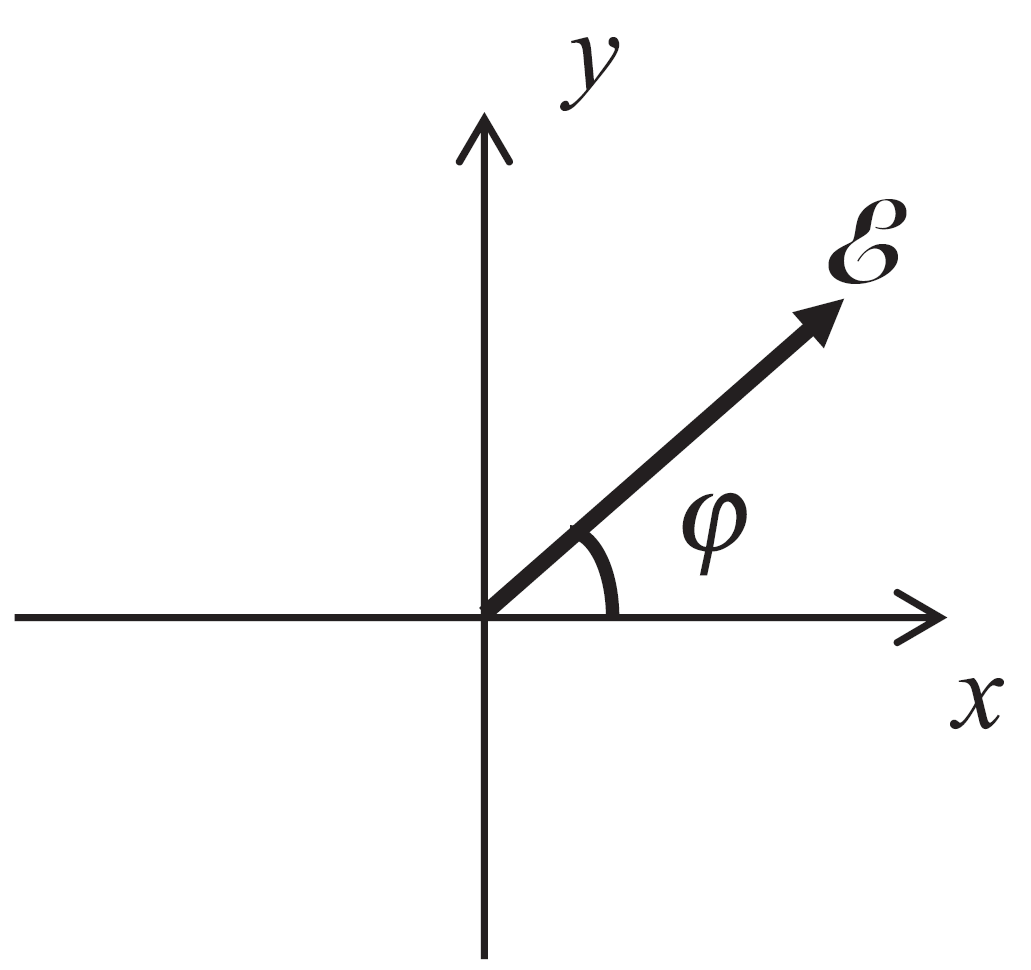
\includegraphics[width=0.2\textwidth]{均匀平面波中的电场方向.PNG}
    \caption{均匀平面波中的电场方向}
    \label{fig:fig40}
\end{figure}
\\
其电场为:
\begin{align}
    \label{eq:eq356}
    \mathbf{E}=\mathbf{E}_0e^{-j\beta z}=(\hat{x}E_{0x}+\hat{y}E_{0y})e^{-j\beta z}
\end{align}
电场在$z$方向没有分量是因为需要满足散度条件$\nabla\cdot\mathbf{E}=0$。其瞬时值为:
\begin{align}
    \label{eq:eq357}
    \mathcal{\vec{E}}(t)&=Re[(\hat{x}E_{0x}+\hat{y}E_{0y})e^{-j\beta z}] \nonumber \\
                        &=\hat{x}|E_{0x}|\cos(wt-\beta z+\angle E_{0x})+\hat{y}|E_{0y}|\cos(wt-\beta z+\angle E_{0y})
\end{align}
电场与$x$轴的夹角为
\begin{align}
    \label{eq:eq358}
    \varphi(t)=\arctan\frac{|E_{0y}|\cos(wt-\beta z+\angle E_{0y})}{|E_{0x}|\cos(wt-\beta z+\angle E_{0x})}
\end{align}
\par
当$\angle E_{0x}=\angle E_{0y}$时,电场矢量总在一条直线上,称为线极化波。对应的磁场为:
\begin{align}
    \label{eq:eq359}
    \mathcal{\vec{H}}(t)=\hat{y}\frac{|E_{0x}|}{\eta}\cos(wt-\beta z+\angle E_{0x})-\hat{x}\frac{|E_{0y}|}{\eta}\cos(wt-\beta z+\angle E_{0x})
\end{align}
则能流密度瞬时值为:
\begin{align}
    \label{eq:eq360}
    \mathcal{\vec{S}}(t)&=\mathcal{\vec{E}}(t)\times\mathcal{\vec{H}}(t)=\hat{z}\frac{|E_{0x}|^2+|E_{0y}|^2}{\eta}\cos^2(wt-\beta z+\angle E_{0x}) \nonumber \\
                        &=\hat{z}\frac{|E_0|^2}{\eta}\cos^2(wt-\beta z+\angle E_{0x})
\end{align}
其在一个周期内的时均值为$|E_0|^2/2\eta$。\par
当$\angle E_{0x}-\angle E_{0y}=\pi/2$时,电场为:
\begin{align}
    \label{eq:eq361}
    \mathcal{\vec{E}}(t)=\hat{x}|E_{0x}|\cos(wt-\beta z+\angle E_{0x})+\hat{y}|E_{0y}|\sin(wt-\beta z+\angle E_{0x})
\end{align}
由此可得
\begin{align}
    \label{eq:eq362}
    \left(\frac{\mathcal{E}_x}{|E_{0x}|}\right)^2+\left(\frac{\mathcal{E}_y}{|E_{0y}|}\right)^2=1
\end{align}
此时电场矢量的终端随时间变化的轨迹是一个椭圆,称为椭圆极化。式\ref{eq:eq358}重新写成
\begin{align}
    \label{eq:eq363}
    \varphi(t)=\arctan\frac{|E_{0y}|\sin(wt-\beta z+\angle E_{0x})}{|E_{0x}|\cos(wt-\beta z+\angle E_{0x})}
\end{align}
固定$z$,沿着传播方向$z$看,随着时间的增加,电场沿着顺时针方向旋转,称为顺时针椭圆极化。如果$|E_{0x}|=|E_{0y}|$,电磁波称为顺时针圆极化。类似的,如果$\angle E_{0x}-\angle E_{0y}=-\pi/2$且$|E_{0x}|\neq|E_{0y}|$时,电磁波为逆时针椭圆极化;如果$\angle E_{0x}-\angle E_{0y}=-\pi/2$且$|E_{0x}|=|E_{0y}|$时,电磁波为逆时针圆极化。
\par
对于圆极化,其磁场瞬时值为:
\begin{align}
    \label{eq:eq364}
    \mathcal{\vec{H}}(t)=\hat{y}\frac{|E_{0x}|}{\eta}\cos(wt-\beta z+\angle E_{0x})\pm\hat{x}\frac{|E_{0x}|}{\eta}\cos(wt-\beta z+\angle E_{0x})
\end{align}
则能流密度瞬时值为:
\begin{align}
    \label{eq:eq365}
    \mathcal{\vec{S}}(t)=\mathcal{\vec{E}}(t)\times\mathcal{\vec{H}}(t)=\hat{z}\frac{|E_0|^2}{\eta}
\end{align}
因此,最大幅度相同的圆极化波和线极化波相比,圆极化波的能流密度是线极化波能流密度时均值的两倍。\par
对于更一般的情况,假设$\angle E_{0x}-\angle E_{0y}=\vartheta(-\pi<\vartheta\leq\pi)$,则电场的瞬时值为:
\begin{align}
    \label{eq:eq366}
    \mathcal{\vec{E}}(t)=\hat{x}|E_{0x}|\cos(wt-\beta z+\angle E_{0x})+\hat{y}|E_{0y}|\cos(wt-\beta z+\angle E_{0x}-\vartheta)
\end{align}
由此可得
\begin{align}
    \label{eq:eq367}
    \left(\frac{\mathcal{E}_x}{|E_{0x}|}\right)^2-\frac{2\mathcal{E}_x\mathcal{E}_y\cos\vartheta}{|E_{0x}||E_{0y}|}+\left(\frac{\mathcal{E}_y}{|E_{0y}|}\right)^2=1
\end{align}
上式描述的电场终端随时间变化的轨迹如图\ref{fig:fig41}所示。其旋转方向取决于$\vartheta$,如果$\vartheta<0$,则为左旋椭圆极化,如果$\vartheta>0$,则为右旋椭圆极化。
\begin{figure}[ht]
    \centering
    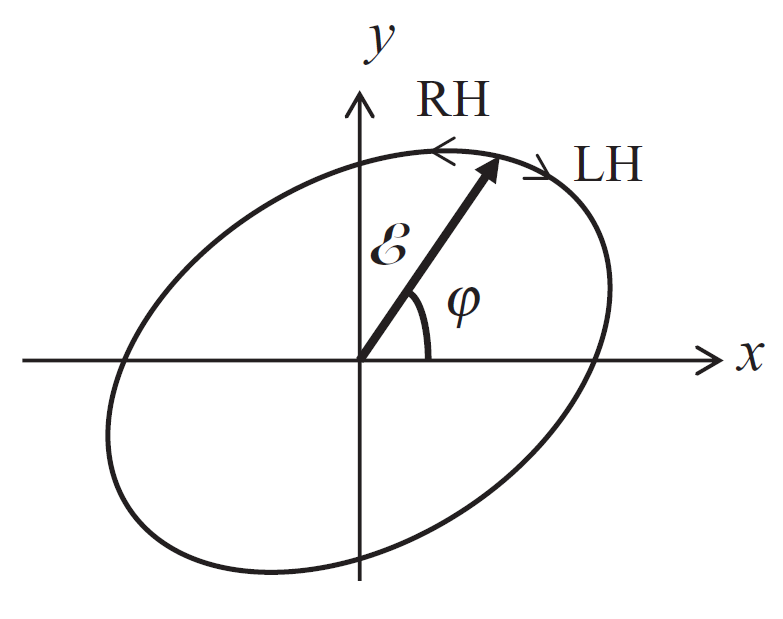
\includegraphics[width=0.3\textwidth]{更一般的左旋或右旋椭圆极化.PNG}
    \caption{更一般的左旋或右旋椭圆极化}
    \label{fig:fig41}
\end{figure}
\par
椭圆极化波或圆极化波可以堪称两个线极化波的叠加,一个线极化波可以分解成两个旋转方向相反的椭圆极化波或圆极化波。
\subsubsection{电磁波在超材料中的传播}
考虑介电常数$\epsilon=\epsilon'$,磁导率$\mu=-\mu'$的媒质,或介电常数$\epsilon=-\epsilon'$,磁导率$\mu=\mu'$的媒质,其中$\epsilon'>0$,$\mu'>0$。在这样的媒质中,色散关系为$\gamma^2=w^2\mu'\epsilon'$,故$\gamma=\alpha=w\sqrt{\mu'\epsilon'}$。因此,虽然媒质无耗,但平面波仍有衰减,无法传播。\par
考虑介电常数$\epsilon=-\epsilon'$,磁导率$\mu=-\mu'$的媒质,此时$\beta=w\sqrt{\mu'\epsilon'}$,因此平面波在该媒质中可以无衰减地传播。若存在一个沿$\hat{beta}$方向传播的平面波,则根据麦克斯韦旋度方程,有
\begin{align}
    \label{eq:eq368}
    \vec{\beta}\times\mathbf{E}=-w\mu'\mathbf{H}\qquad\vec{\beta}\times\mathbf{H}=w\epsilon'\mathbf{E}
\end{align}
此时电场矢量、磁场矢量、波矢量满足左手定则。又
\begin{align}
    \label{eq:eq369}
    \mathbf{E}\times\mathbf{H}^*=-\hat{\beta}\sqrt{\frac{\epsilon'}{\mu'}}|E|^2
\end{align}
因此,能量传播方向与相速方向相反。需要注意的是,在左手媒质中,传播常数$\gamma$应该选择$\gamma=\alpha-j\beta$,即选择能流方向而不是相速方向。为了保证功率从源向远处传播,无界均匀左手媒质中的标量格林函数应该为:
\begin{align}
    \label{eq:eq370}
    G_0(\vec{r},\vec{r}')=\frac{e^{jk|\vec{r}-\vec{r}'|}}{4\pi |\vec{r}-\vec{r}'|}
\end{align}
其中$k=w\sqrt{\mu'\epsilon'}$。
\subsection{面电流产生的平面波}
考虑一个位于$xy$平面的无限大面电流,处于介电常数为$\epsilon$,磁导率为$\mu$的无界均匀媒质中。如图\ref{fig:fig42}所示。
\begin{figure}[ht]
    \centering
    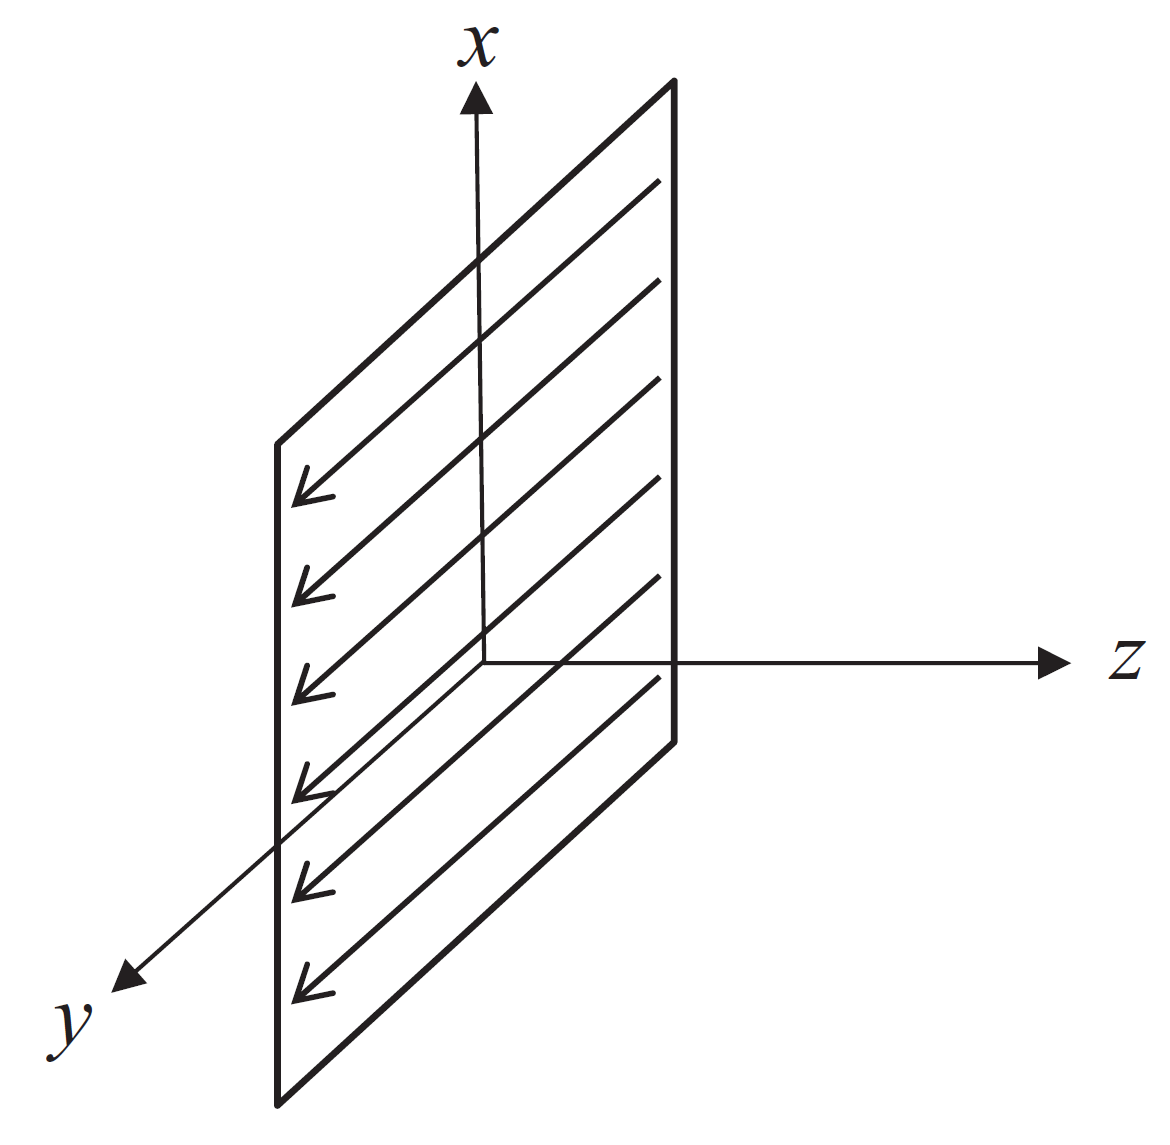
\includegraphics[width=0.3\textwidth]{位于xy平面的无限大面电流.PNG}
    \caption{位于$xy$平面的无限大面电流}
    \label{fig:fig42}
\end{figure}
\\
面电流密度为
\begin{align}
    \label{eq:eq371}
    \mathbf{J}_S=\hat{y}J_0e^{-jhx}
\end{align}
其中$J_0$为常数。在$xy$以外的区域,场满足式\ref{eq:eq320}、式\ref{eq:eq321}给出的无源区域矢量亥姆霍兹方程,其解由式\ref{eq:eq331}、式\ref{eq:eq332}给出。由于$\hat{z}\times[\mathbf{H}(z=0+)-\mathbf{H}(z=0-)]=\mathbf{J}_S$,则磁场可表示为
\begin{align}
    \label{eq:eq372}
    \mathbf{H}=
    \left\{
        \begin{array}{lr}
            \mathbf{A}e^{-jhx+j\beta_zz}, &z<0 \\
            \mathbf{B}e^{-jhx-j\beta_zz}, &z>0
        \end{array}
    \right.
\end{align}
其中$\mathbf{A}$、$\mathbf{B}$待定,$\beta_z=\sqrt{w^2\mu\epsilon-h^2}$,根据边界条件,在原点处,有
\begin{align}
    \label{eq:eq373}
    B_x-A_x&=J_0 \\
    \label{eq:eq374}
    B_y-A_y&=0
\end{align}
在无源区域,有$\nabla\cdot\mathbf{H}=0$,即
\begin{align}
    \label{eq:eq375}
    hB_x+\beta_zB_z&=0 \\
    \label{eq:eq376}
    hA_x-\beta_zA_z&=0
\end{align}
由$\nabla\times\mathbf{H}=jw\epsilon\mathbf{E}$得,
\begin{align}
    \label{eq:eq377}
    \mathbf{E}=-\frac{1}{w\epsilon}
    \left\{
        \begin{array}{lr}
            (\hat{x}h-\hat{z}\beta_z)\times\mathbf{A}e^{-jhx+j\beta_zz}, &z<0 \\
            (\hat{x}h+\hat{z}\beta_z)\times\mathbf{B}e^{-jhx-j\beta_zz}, &z>0
        \end{array}
    \right.
\end{align}
由于$xy$平面两侧电场连续,即$\hat{z}\times[\mathbf{E}(z=0+)-\mathbf{E}(z=0-)]=0$,则有
\begin{align}
    \label{eq:eq378}
    hB_z+\beta_zB_x&=hA_z+\beta_zA_x \\
    \label{eq:eq379}
    B_y+A_y&=0
\end{align}
联立式\ref{eq:eq373}、式\ref{eq:eq374}、式\ref{eq:eq375}、式\ref{eq:eq376}、式\ref{eq:eq378}、式\ref{eq:eq379},得
\begin{align}
    \label{eq:eq380}
    B_x=-A_x=\frac{J_0}{2}\qquad B_y=A_y=0\qquad B_z=A_z=-\frac{h}{\beta_z}\frac{J_0}{2}
\end{align}
故,面电流产生的电场和磁场分别为
\begin{align}
    \label{eq:eq381}
    \mathbf{E}&=-\hat{y}\frac{w\mu J_0}{x\beta_z}
    \left\{
        \begin{array}{lr}
            e^{-jhx+j\beta_zz}, &z<0 \\
            e^{-jhx-j\beta_zz}, &z>0
        \end{array}
    \right. \\
    \label{eq:eq382}
    \mathbf{H}&=\frac{J_0}{x\beta_z}
    \left\{
        \begin{array}{lr}
            (-\hat{x}\beta_z-\hat{z}h)e^{-jhx+j\beta_zz}, &z<0 \\
            (\hat{x}\beta_z-\hat{z}h)e^{-jhx-j\beta_zz}, &z>0
        \end{array}
    \right.
\end{align}
在$z<0$和$z>0$的区域,波的传播方向分别为$\vec{\beta}=\hat{x}h-\hat{z}\beta_z$,$\vec{\beta}=\hat{x}h+\hat{z}\beta_z$,均受$h$控制。\\
对于特殊问题,按照以下步骤求解: \\
(1)基于无源区域的通解,写出包含待定系数的电场或磁场表达式; \\
(2)根据麦克斯韦方程导出另一个场量的表达式; \\
(3)应用边界条件确定待定系数。 \\
\subsection{反射和透射}
假设存在两种各向同性媒质,其分界面为$xy$平面,在$z<0$的空间中,媒质介电常数为$\epsilon_1$,磁导率为$\mu_1$,在$z>0$的空间中,媒质介电常数为$\epsilon_2$,磁导率为$\mu_2$。
\subsubsection{垂直入射波}
考虑一沿$z$方向传播的平面波,从$z<0$的区域入射到分界面上,如图\ref{fig:fig43}所示。
\begin{figure}[ht]
    \centering
    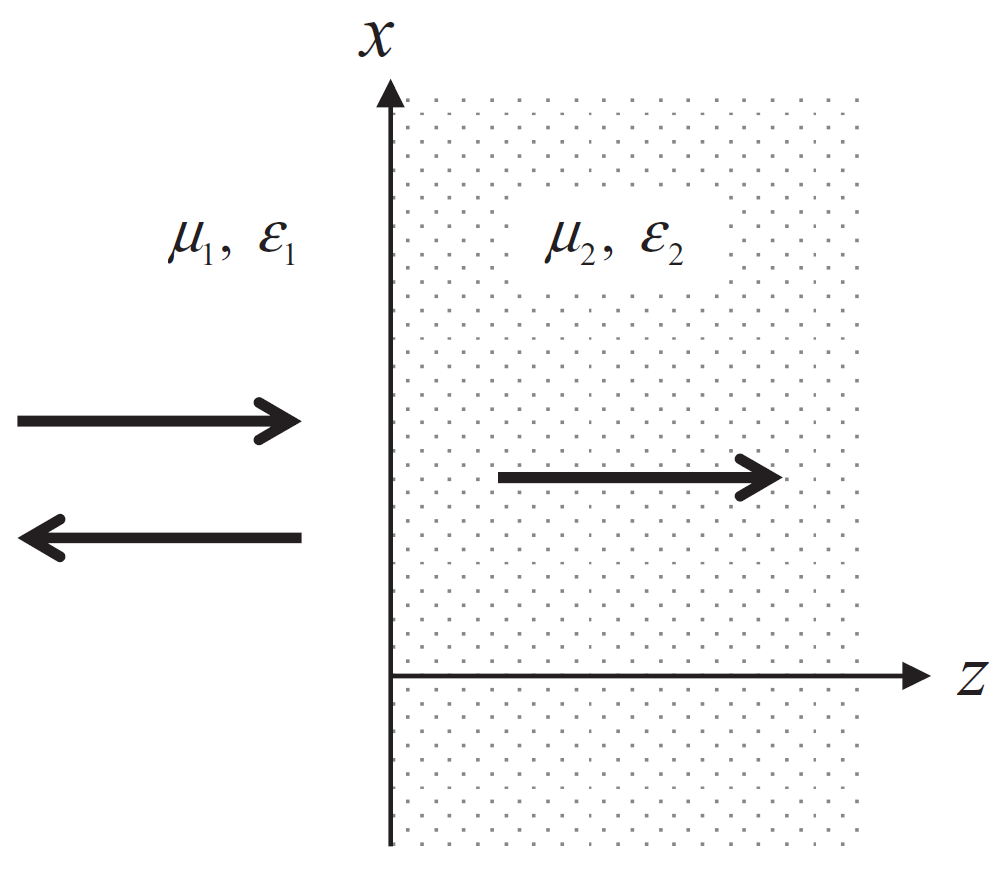
\includegraphics[width=0.3\textwidth]{平面波垂直入射到分界面上.PNG}
    \caption{平面波垂直入射到分界面上}
    \label{fig:fig43}
\end{figure}
\\
则入射波、反射波、透射波的电场分别为:
\begin{align}
    \label{eq:eq383}
    \mathbf{E}^i&=\hat{x}E_0e^{-j\beta_1z} \\
    \label{eq:eq384}
    \mathbf{E}^r&=\hat{x}RE_0e^{j\beta_1z} \\
    \label{eq:eq385}
    \mathbf{E}^t&=\hat{x}TE_0e^{-j\beta_2z}
\end{align}
式中,$\beta_1=w\sqrt{\mu_1\epsilon_1}$,$\beta_2=w\sqrt{\mu_2\epsilon_2}$,$R$和$T$分别为待定的反射系数和投射系数。根据麦克斯韦方程$\nabla\times\mathbf{E}=-jw\mu\mathbf{H}$得,相应的磁场为:
\begin{align}
    \label{eq:eq386}
    \mathbf{H}^i&=\hat{y}\frac{E_0}{\eta_1}e^{-j\beta_1z} \\
    \label{eq:eq387}
    \mathbf{H}^r&=-\hat{y}\frac{RE_0}{\eta_1}e^{j\beta_1z} \\
    \label{eq:eq388}
    \mathbf{H}^t&=\hat{y}\frac{TE_0}{\eta_2}e^{-j\beta_2z}
\end{align}
式中,$\eta_1=\sqrt{\mu_1/\epsilon_1}$,$\eta_2=\sqrt{\mu_2/\epsilon_2}$。分界面上没有面电流和面磁流,所以分界面两边电场和磁场连续,即$\hat{z}\times\mathbf{E}(z=0_+)=\hat{z}\times\mathbf{E}(z=0_-)$,$\hat{z}\times\mathbf{H}(z=0_+)=\hat{z}\times\mathbf{H}(z=0_-)$,由此可得
\begin{align}
    \label{eq:eq389}
    1+R&=T \\
    \label{eq:eq390}
    \frac{1}{\eta_1}(1-R)&=\frac{1}{\eta_2}T
\end{align}
解得
\begin{align}
    \label{eq:eq391}
    R&=\frac{\eta_2-\eta_1}{\eta_2+\eta_1} \\
    \label{eq:eq392}
    T&=\frac{2\eta_2}{\eta_2+\eta_1}
\end{align}
因此,当$\eta_1=\eta_2$时,$R=0$,$T=1$;若媒质2是理想导体,即$\eta_2=0$时,$R=-1$,$T=0$,此时,空间1中的电场和磁场分别为:
\begin{align}
    \label{eq:eq393}
    \mathbf{E}&=\mathbf{E}^i+\mathbf{E}^r=\hat{x}E_0(e^{-j\beta_1z}-e^{j\beta_1z})=-\hat{x}2jE_0\sin\beta_1z \\
    \label{eq:eq394}
    \mathbf{H}&=\mathbf{H}^i+\mathbf{H}^r=\hat{y}\frac{E_0}{\eta_1}(e^{-j\beta_1z}+e^{j\beta_1z})=\hat{y}\frac{2E_0}{\eta_1}\cos\beta_1z
\end{align}
坡印廷矢量为:
\begin{align}
    \label{eq:eq395}
    \mathbf{S}=\frac{1}{2}\mathbf{E}\times\mathbf{H}^*=\hat{z}\frac{|E_0|^2}{j\eta_1}\sin(2\beta_1z)
\end{align}
实部为零,即能流密度时均值为零,这样的波称为纯\textbf{\color{blue}{驻波}}。
对于一般情况,即$\eta_1\neq\eta_2$,$\eta_2\neq0$时,$z<0$区域的电场为:
\begin{align}
    \label{eq:eq396}
    \mathbf{E}&=\mathbf{E}^i+\mathbf{E}^r=\hat{x}E_0(e^{-j\beta_1z}+Re^{j\beta_1z})
\end{align}
其幅度
\begin{align}
    \label{eq:eq397}
    |E|=|E_0|\sqrt{1+|R|^2+2|R|\cos(2\beta_1z+\angle R)}
\end{align}
上式为一个一般的驻波,其\textbf{\color{blue}{驻波比}}(SWR)为:
\begin{align}
    \label{eq:eq398}
    SWR=\frac{|E|_{max}}{|E|_{min}}=\frac{1+|R|}{1-|R|}
\end{align}
将式\ref{eq:eq396}写成
\begin{align}
    \label{eq:eq399}
    \mathbf{E}=\hat{x}E_0(e^{-j\beta_1z}+e^{j\beta_1z})+\hat{x}(1-R)E_0e^{-j\beta_1z}
\end{align}
即总场可以看成纯驻波和行波的叠加,其能流密度时均值由行波贡献,为:
\begin{align}
    \label{eq:eq400}
    Re(\mathbf{S})=\hat{z}\frac{|E_0|^2}{2\eta_1}(1-|R|^2)
\end{align}
\subsubsection{斜入射波}
定义\textbf{\color{blue}{入射平面}}为分界面法向矢量和入射波波矢量确定的平面。因为任何均匀平面波都可以分解成两个相互正交的线极化波的叠加,因此只考虑两种线极化入射波的情况:第一种线极化波的电场垂直于入射平面,这种情况称为\textbf{\color{blue}{垂直极化入射}};第二种线极化波的电场平行于入射平面,这种情况称为\textbf{\color{blue}{平行极化入射}}。
\\
(1)垂直极化入射\par
垂直极化平面波斜入射问题的几何图示如图\ref{fig:fig44}。
\begin{figure}[ht]
    \centering
    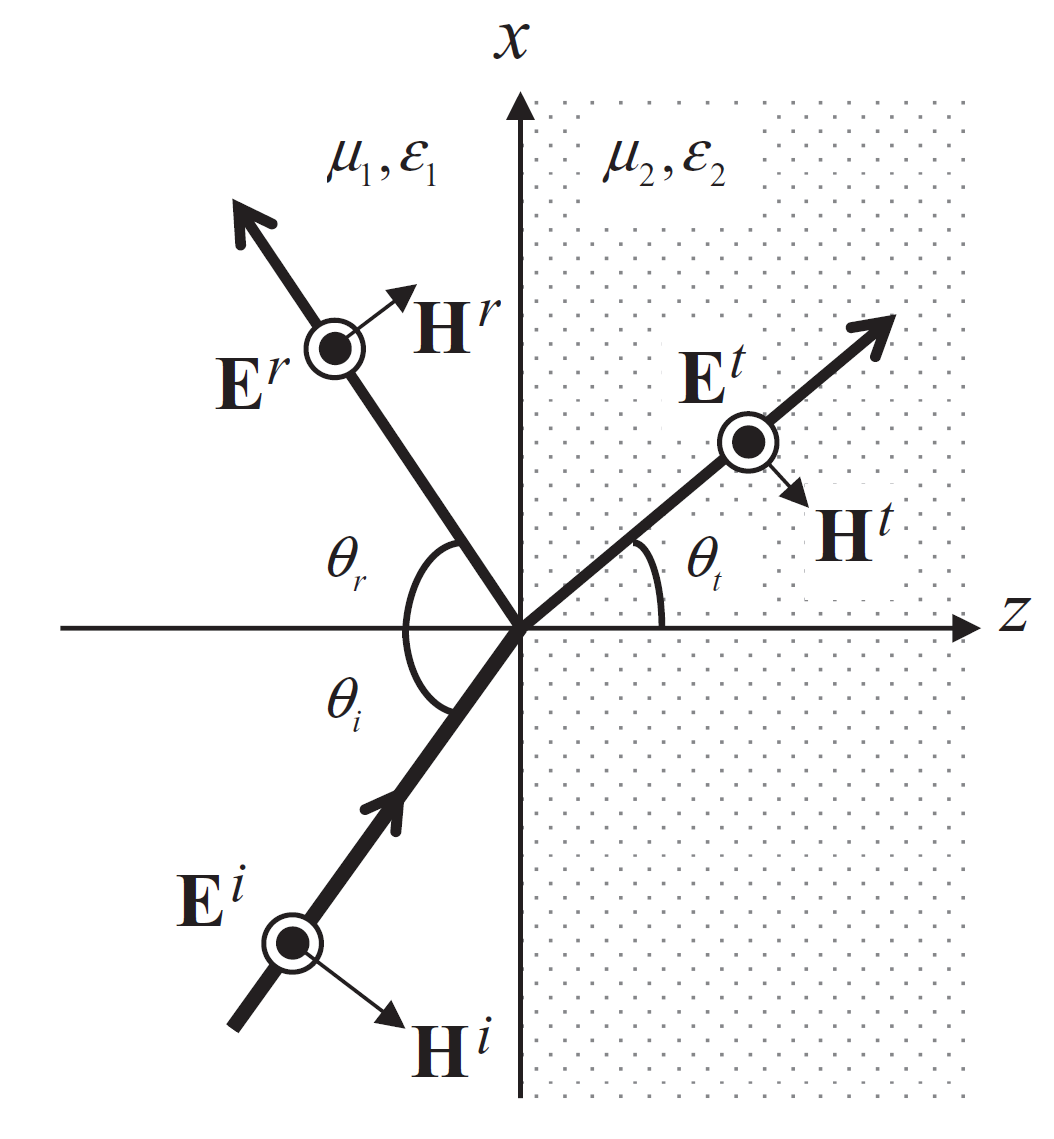
\includegraphics[width=0.3\textwidth]{垂直极化平面波的斜入射问题.PNG}
    \caption{垂直极化平面波的斜入射问题}
    \label{fig:fig44}
\end{figure}
\\
则入射波、反射波、透射波的电场表达式为:
\begin{align}
    \label{eq:eq401}
    \mathbf{E}^i&=\hat{y}E_0e^{-j\vec{\beta}^i\cdot\vec{r}}=\hat{y}E_0e^{-j\beta_1(x\sin\theta_i+z\cos\theta_i)} \\
    \label{eq:eq402}
    \mathbf{E}^r&=\hat{y}R_{\perp}E_0e^{-j\vec{\beta}^r\cdot\vec{r}}=\hat{y}R_{\perp}E_0e^{-j\beta_1(x\sin\theta_r-z\cos\theta_r)} \\
    \label{eq:eq403}
    \mathbf{E}^t&=\hat{y}T_{\perp}E_0e^{-j\vec{\beta}^t\cdot\vec{r}}=\hat{y}T_{\perp}E_0e^{-j\beta_2(x\sin\theta_t+z\cos\theta_t)}
\end{align}
其中$R_{\perp}$、$T_{\perp}$是待定反射和透射系数,$\theta_i$是已知的入射角度,$\theta_r$、$\theta_t$分别是待定的反射角度、透射角度。由$\nabla\times\mathbf{E}=-jw\mu\mathbf{H}$得入射波、反射波、透射波的磁场表达式为:
\begin{align}
    \label{eq:eq404}
    \mathbf{H}^i&=(-\hat{x}\cos\theta_i+\hat{z}\sin\theta_i)\frac{E_0}{\eta_1}e^{-j\beta_1(x\sin\theta_i+z\cos\theta_i)} \\
    \label{eq:eq405}
    \mathbf{H}^r&=(\hat{x}\cos\theta_r+\hat{z}\sin\theta_r)\frac{R_{\perp}E_0}{\eta_1}e^{-j\beta_1(x\sin\theta_r-z\cos\theta_r)} \\
    \label{eq:eq406}
    \mathbf{H}^t&=(-\hat{x}\cos\theta_t+\hat{z}\sin\theta_t)\frac{T_{\perp}E_0}{\eta_2}e^{-j\beta_2(x\sin\theta_t+z\cos\theta_t)}
\end{align}
分界面上没有面电流和面磁流,所以分界面两边电场和磁场连续,即$\hat{z}\times\mathbf{E}(z=0_+)=\hat{z}\times\mathbf{E}(z=0_-)$,$\hat{z}\times\mathbf{H}(z=0_+)=\hat{z}\times\mathbf{H}(z=0_-)$,由此可得
\begin{align}
    \label{eq:eq407}
    e^{-j\beta_1\sin\theta_ix}+R_{\perp}e^{-j\beta_1\sin\theta_rx}&=T_{\perp}e^{-j\beta_2\sin\theta_tx} \\
    \label{eq:eq408}
    \cos\theta_i\frac{1}{\eta_1}e^{-j\beta_1\sin\theta_ix}+\cos\theta_r\frac{R_{\perp}}{\eta_1}e^{-j\beta_1\sin\theta_rx}&=\cos\theta_t\frac{T_{\perp}}{\eta_2}e^{-j\beta_2\sin\theta_tx}
\end{align}
上面两个等式对任意$x$成立,则有
\begin{align}
    \label{eq:eq409}
    \beta_1\sin\theta_i=\beta_1\sin\theta_r=\beta_2\sin\theta_t
\end{align}
上式称为\textbf{\color{blue}{相位匹配条件}}。由$\beta_1=w\sqrt{\mu_1\epsilon_1}$,$\beta_2=w\sqrt{\mu_2\epsilon_2}$得
\begin{align}
    \label{eq:eq410}
    \theta_r=\theta_i\qquad\frac{\sin\theta_t}{\sin\theta_i}=\sqrt{\frac{\mu_1\epsilon_1}{\mu_2\epsilon_2}}
\end{align}
上式称为\textbf{\color{blue}{斯奈尔反射和折射定律}}。将式\ref{eq:eq409}代入式\ref{eq:eq407}、式\ref{eq:eq408},得
\begin{align}
    \label{eq:eq411}
    1+R_{\perp}&=T_{\perp} \\
    \label{eq:eq412}
    \cos\theta_i\frac{1}{\eta_1}-\cos\theta_r\frac{R_{\perp}}{\eta_1}&=\cos\theta_t\frac{T_{\perp}}{\eta_2}
\end{align}
解得
\begin{align}
    \label{eq:eq413}
    R_{\perp}&=\frac{\eta_2\cos\theta_i-\eta_1\cos\theta_t}{\eta_2\cos\theta_i+\eta_1\cos\theta_t} \\
    \label{eq:eq414}
    T_{\perp}&=\frac{2\eta_2\cos\theta_i}{\eta_2\cos\theta_i+\eta_1\cos\theta_t}
\end{align}
定义向$z$方向看入的波阻抗为$Z_z=-E_y/H_x$,则两个区域的波阻抗分别为:
\begin{align}
    \label{eq:eq415}
    Z_{z1}=\frac{\eta_1}{\cos\theta_i}\qquad Z_{z2}=\frac{\eta_2}{\cos\theta_t}
\end{align}
因此,式\ref{eq:eq413}、式\ref{eq:eq414}可重写为
\begin{align}
    \label{eq:eq416}
    R_{\perp}&=\frac{Z_{z2}-Z_{z1}}{Z_{z2}+Z_{z1}} \\
    \label{eq:eq417}
    T_{\perp}&=\frac{2Z_{z2}}{Z_{z2}+Z_{z1}}
\end{align}
(2)平行极化入射\par
垂直极化平面波斜入射问题的几何图示如图\ref{fig:fig45}。
\begin{figure}[ht]
    \centering
    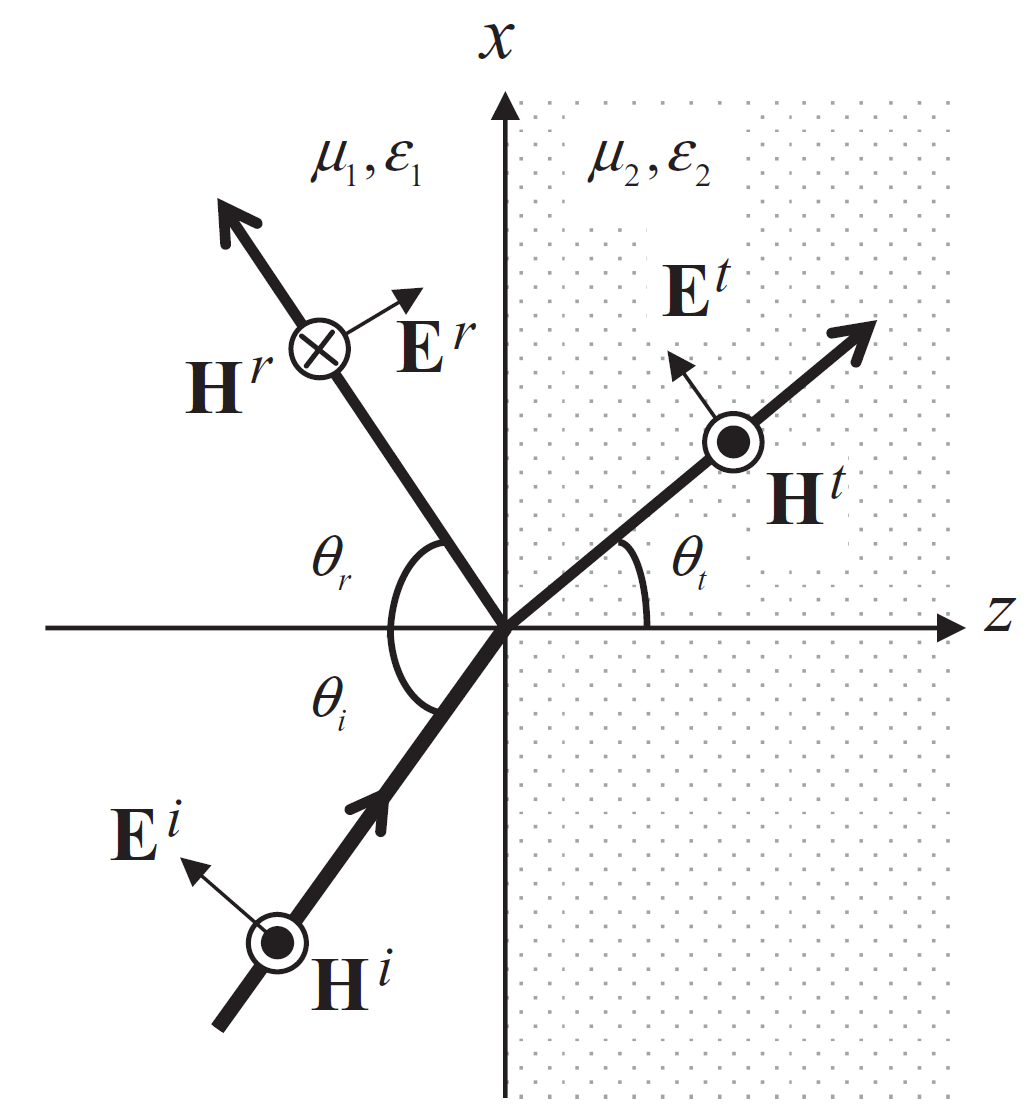
\includegraphics[width=0.3\textwidth]{平行极化平面波的斜入射问题.PNG}
    \caption{平行极化平面波的斜入射问题}
    \label{fig:fig45}
\end{figure}
\\
则入射波、反射波、透射波的电场表达式为:
\begin{align}
    \label{eq:eq418}
    \mathbf{E}^i&=(\hat{x}\cos\theta_i-\hat{z}\sin\theta_i)E_0e^{-j\beta_1(x\sin\theta_i+z\cos\theta_i)} \\
    \label{eq:eq419}
    \mathbf{E}^r&=(\hat{x}\cos\theta_r+\hat{z}\sin\theta_r)R_{\parallel}E_0e^{-j\beta_1(x\sin\theta_r-z\cos\theta_r)} \\
    \label{eq:eq420}
    \mathbf{E}^t&=(\hat{x}\cos\theta_t-\hat{z}\sin\theta_t)T_{\parallel}E_0e^{-j\beta_2(x\sin\theta_t+z\cos\theta_t)}
\end{align}
其中$R_{\parallel}$、$T_{\parallel}$是待定反射和透射系数,$\theta_i$是已知的入射角度,$\theta_r$、$\theta_t$分别是待定的反射角度、透射角度。由$\nabla\times\mathbf{E}=-jw\mu\mathbf{H}$得入射波、反射波、透射波的磁场表达式为:
\begin{align}
    \label{eq:eq421}
    \mathbf{H}^i&=\hat{y}\frac{E_0}{\eta_1}e^{-j\beta_1(x\sin\theta_i+z\cos\theta_i)} \\
    \label{eq:eq422}
    \mathbf{H}^r&=-\hat{y}\frac{R_{\parallel}E_0}{\eta_1}e^{-j\beta_1(x\sin\theta_r-z\cos\theta_r)} \\
    \label{eq:eq423}
    \mathbf{H}^t&=\hat{y}\frac{T_{\parallel}E_0}{\eta_2}e^{-j\beta_2(x\sin\theta_t+z\cos\theta_t)}
\end{align}
分界面上没有面电流和面磁流,所以分界面两边电场和磁场连续,即$\hat{z}\times\mathbf{E}(z=0_+)=\hat{z}\times\mathbf{E}(z=0_-)$,$\hat{z}\times\mathbf{H}(z=0_+)=\hat{z}\times\mathbf{H}(z=0_-)$,由此可得
\begin{align}
    \label{eq:eq424}
    \cos\theta_ie^{-j\beta_1\sin\theta_ix}+\cos\theta_rR_{\parallel}e^{-j\beta_1\sin\theta_rx}&=\cos\theta_tT_{\parallel}e^{-j\beta_2\sin\theta_tx} \\
    \label{eq:eq425}
    \frac{1}{\eta_1}e^{-j\beta_1\sin\theta_ix}-\frac{R_{\parallel}}{\eta_1}e^{-j\beta_1\sin\theta_rx}&=\frac{T_{\parallel}}{\eta_2}e^{-j\beta_2\sin\theta_tx}
\end{align}
上面两个等式对任意$x$成立,则同样需要满足相位匹配条件,从而得到平行波入射同样遵循斯奈尔反射和折射定律。将式\ref{eq:eq409}代入式\ref{eq:eq424}、式\ref{eq:eq425},得
\begin{align}
    \label{eq:eq428}
    \cos\theta_i+\cos\theta_rR_{\parallel}&=\cos\theta_tT_{\parallel} \\
    \label{eq:eq429}
    \frac{1}{\eta_1}-\frac{R_{\parallel}}{\eta_1}&=\frac{T_{\parallel}}{\eta_2}
\end{align}
解得
\begin{align}
    \label{eq:eq430}
    R_{\parallel}&=\frac{\eta_2\cos\theta_t-\eta_1\cos\theta_i}{\eta_2\cos\theta_t+\eta_1\cos\theta_i} \\
    \label{eq:eq431}
    T_{\parallel}&=\frac{2\eta_2\cos\theta_i}{\eta_2\cos\theta_t+\eta_1\cos\theta_i}
\end{align}
定义向$z$方向看入的波阻抗为$Z_z=E_x/H_y$,则两个区域的波阻抗分别为:
\begin{align}
    \label{eq:eq432}
    Z_{z1}=\eta_1{\cos\theta_i}\qquad Z_{z2}=\eta_2{\cos\theta_t}
\end{align}
因此,式\ref{eq:eq430}、式\ref{eq:eq431}可重写为
\begin{align}
    \label{eq:eq433}
    R_{\parallel}&=\frac{Z_{z2}-Z_{z1}}{Z_{z2}+Z_{z1}} \\
    \label{eq:eq434}
    T_{\parallel}&=\frac{2Z_{z2}}{Z_{z2}+Z_{z1}}
\end{align}
\par
当右半空间为理想导体,即$\eta_2$时,无论对于哪种极化,在分界面上均有
\begin{align}
    \label{eq:eq435}
    \hat{n}\times\mathbf{H}=\hat{n}\times(\mathbf{H}^i+\mathbf{H}^r)=2\hat{n}\times\mathbf{H}^i
\end{align}
因此,对于电大尺寸的光滑导体表面,任意入射平面波的感应电流为:
\begin{align}
    \label{eq:eq436}
    \mathbf{J}_S\approx2\hat{n}\times\mathbf{H}^i
\end{align}
即物理光学近似。\par
进一步分析式\ref{eq:eq413}、式\ref{eq:eq414}和式\ref{eq:eq430}、式\ref{eq:eq431}。当反射系数为0,发生\textbf{\color{blue}{全透射}}现象时,对应的入射角称为\textbf{\color{blue}{布儒斯特角}},记为$\theta_B$。对于垂直极化,全透射的条件为:
\begin{align}
    \label{eq:eq437}
    \eta_2\cos\theta_B=\eta_1\cos\theta_t
\end{align}
联立斯奈尔折射定律,解得
\begin{align}
    \label{eq:eq438}
    \sin\theta_B=\sqrt{\frac{\epsilon_2/\epsilon_1-\mu_2/\mu_1}{\mu_1/\mu_2-\mu_2/\mu_1}}
\end{align}
对于平行极化,全透射的条件为:
\begin{align}
    \label{eq:eq439}
    \eta_2\cos\theta_t=\eta_1\cos\theta_B
\end{align}
联立斯奈尔折射定律,解得
\begin{align}
    \label{eq:eq440}
    \sin\theta_B=\sqrt{\frac{\epsilon_2/\epsilon_1-\mu_2/\mu_1}{\epsilon_2/\epsilon_1-\epsilon_1/\epsilon_2}}
\end{align}
考虑斯奈尔折射定律,当$\sin\theta_i=\sqrt{\mu_2\epsilon_2/\mu_1\epsilon_1}$时,$\theta_t=\pi/2$,此时$R_{\perp}=1$,$R_{\parallel}=-1$,这种现象称为\textbf{\color{blue}{全反射}},相应的入射角称为\textbf{\color{blue}{临界角}}:
\begin{align}
    \label{eq:eq441}
    \theta_c=\arcsin\sqrt{\frac{\mu_2\epsilon_2}{\mu_1\epsilon_1}}
\end{align}
只有当$\mu_1\epsilon_1>\mu_2\epsilon_2$时,临界角才存在。当$\theta_i=\theta_c$时,垂直极化波对应的透射场为:
\begin{align}
    \label{eq:eq442}
    \mathbf{E}^t=\hat{y}2E_0e^{-j\beta_2x}
\end{align}
平行极化波对应的透射场为:
\begin{align}
    \label{eq:eq443}
    \mathbf{E}^t=-\hat{z}2E_0\frac{\eta_2}{\eta_1}e^{-j\beta_2x}
\end{align}
入射波、反射波、透射波的能流密度时均值分别为:
\begin{align}
    \label{eq:eq444}
    \left.\mathbf{S}^i\right|_{\theta_i=\theta_c}&=\hat{\beta}^i\frac{|E_0|^2}{2\eta_1} \\
    \label{eq:eq445}
    \left.\mathbf{S}^r\right|_{\theta_i=\theta_c}&=\hat{\beta}^r\frac{|E_0|^2}{2\eta_1} \\
    \label{eq:eq446}
    \left.\mathbf{S}^t\right|_{\theta_i=\theta_c}&=\hat{\beta}^t\frac{2|E_0|^2}{\eta_2}
\end{align}
当$\theta_i>\theta_c$时,有$\sin\theta_t>1$,$\cos\theta_t=\sqrt{1-\sin^2\theta_t}=\pm j\sqrt{\sin^2\theta_t-1}$(为使结果有物理意义,取负号,即$\cos\theta_t=-j\sqrt{\sin^2\theta_t-1}$),$R_{\perp}$和$R_{\parallel}$均为复数,但仍有$|R_{\perp}|=1$和$|R_{\parallel}=1$,仍发生全反射。此时垂直极化波对应的透射场为:
\begin{align}
    \label{eq:eq447}
    \mathbf{E}^t=\hat{y}T_{\perp}E_0e^{-\alpha_ez}e^{-j\beta_2x\sin\theta_t}
\end{align}
平行极化波对应的透射场为:
\begin{align}
    \label{eq:eq448}
    \mathbf{E}^t=(\hat{x}\cos\theta_t-\hat{z}\sin\theta_t)T_{\parallel}E_0e^{-\alpha_ez}e^{-j\beta_2x\sin\theta_t}
\end{align}
式中,$\alpha_e=\beta_2\sqrt{\sin^2\theta_t-1}$,这两个波均沿着$x$轴传播,但波的幅度在$z$轴方向有衰减,因此,等相面和等幅面不平行,是非均匀平面波。$x$方向的相速为:
\begin{align}
    \label{eq:eq449}
    v_p=\frac{w}{\beta_2\sin\theta_t}
\end{align}
小于相同媒质中均匀平面波的相速,称为慢波。能流时均值仍沿着$x$轴方向,在$z$轴方向存在瞬时能流,但时均值为零。
\subsubsection{电磁波入射到左手媒质}
如图\ref{fig:fig46}所示,右半空间媒质为左手媒质,即$\epsilon_2=-\epsilon_2'$,$\mu_2=-\mu_2'$,其中$\epsilon_2'>0$,$\mu_2'>0$,一个垂直极化波向分界面斜入射。
\begin{figure}[ht]
    \centering
    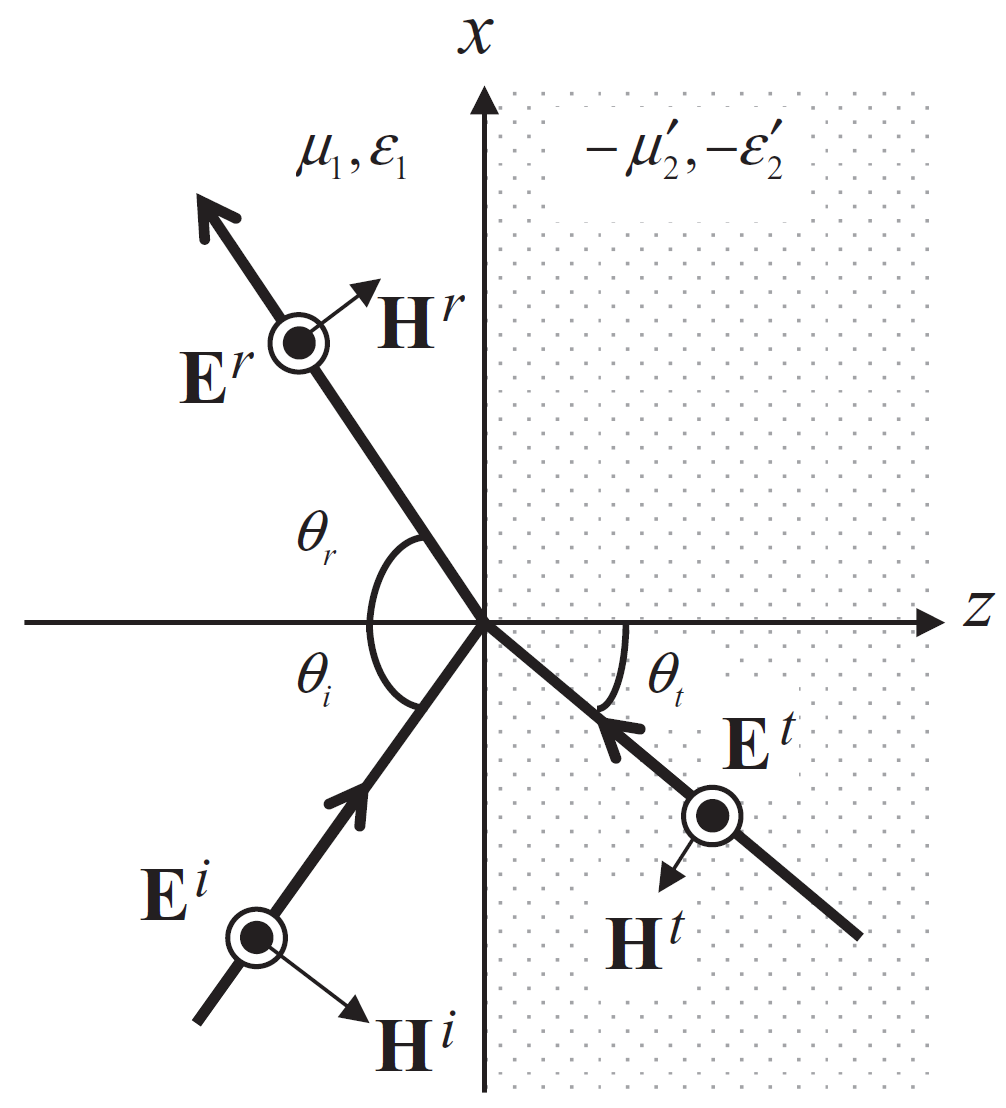
\includegraphics[width=0.3\textwidth]{平面波入射到左手媒质.PNG}
    \caption{平面波入射到左手媒质}
    \label{fig:fig46}
\end{figure}
\\
由于左手媒质中的功率传播方向和相速传播方向相反,透射场的相位必须向着分界面的方向传播,才能保证功率向远离分界面的方向传播。则此时透射波的电场为:
\begin{align}
    \label{eq:eq450}
    \mathbf{E}^t=\hat{y}T_{\perp}E_0e^{-j\vec{\beta}^t\cdot\vec{r}}=\hat{y}T_{\perp}E_0e^{-j\beta_2'(x\sin\theta_t-z\cos\theta_t)}
\end{align}
式中,$\beta_2'=w\sqrt{\mu_2'\epsilon_2'}$。对应磁场为:
\begin{align}
    \label{eq:eq451}
    \mathbf{H}^t=-(\hat{x}\cos\theta_t+\hat{z}\sin\theta_t)\frac{T_{\perp}E_0}{\eta_2}e^{-j\beta_2'(x\sin\theta_t-z\cos\theta_t)}
\end{align}
式中,$\eta_2'=\sqrt{\mu_2'/\epsilon_2'}$。根据相位匹配条件,得
\begin{align}
    \label{eq:eq452}
    \sin\theta_t=\sqrt{\frac{\mu_1\epsilon_1}{\mu_2'\epsilon_2'}}\sin\theta_i
\end{align}
其反射系数与透射系数和右手媒质形式相同,只是$\eta_2=\eta_2'$。如果令$\beta_2=\beta_2'$且$\eta_2=\eta_2'$,则可从右手媒质的场推导左手媒质的场。
\subsection{各向异性媒质中的平面波}
\subsubsection{单轴媒质}
考虑在单轴媒质中传播的平面波,其电场为$\mathbf{E}=\mathbf{E}_0e^{-j\vec{\beta}\cdot\vec{r}}$,媒质的介电常数为:
\begin{align}
    \label{eq:eq453}
    \overline{\vec{\epsilon}}=
        \left[
            \begin{matrix}
                \epsilon & 0 & 0 \\
                0 & \epsilon & 0 \\
                0 & 0 & \epsilon_z \\
            \end{matrix}
        \right]
\end{align}
根据无源区域的麦克斯韦方程
\begin{align}
    \label{eq:eq454}
    \vec{\beta}\times\mathbf{E}&=w\mu\mathbf{H} \\
    \label{eq:eq455}
    \vec{\beta}\times\mathbf{H}&=-w\overline{\vec{\epsilon}}\cdot\mathbf{E}
\end{align}
得
\begin{align}
    \label{eq:eq456}
    \vec{\beta}\times(\vec{\beta}\times\mathbf{E})=-w^2\mu\overline{\vec{\epsilon}}\cdot\mathbf{E}
\end{align}
假设波沿着$x$的方向传播,即$\vec{\beta}=\hat{x}\beta_x$,则上式重写为
\begin{align}
    \label{eq:eq457}
    \left[
        \begin{matrix}
            -w^2\mu\epsilon & 0 & 0 \\
            0 & \beta_x^2-w^2\mu\epsilon & 0 \\
            0 & 0 & \beta_x^2-w^2\mu\epsilon_z \\
        \end{matrix}
    \right]
    \left[
        \begin{matrix}
            E_x \\
            E_y \\
            E_z \\
        \end{matrix}
    \right]=0
\end{align}
显然,有$E_x=0$,则上式简化为
\begin{align}
    \label{eq:eq458}
    \left[
        \begin{matrix}
            \beta_x^2-w^2\mu\epsilon & 0 \\
            0 & \beta_x^2-w^2\mu\epsilon_z \\
        \end{matrix}
    \right]
    \left[
        \begin{matrix}
            E_y \\
            E_z \\
        \end{matrix}
    \right]=0
\end{align}
若方程要有非零解,则
\begin{align}
    \label{eq:eq459}
    \left|
        \begin{matrix}
            \beta_x^2-w^2\mu\epsilon & 0 \\
            0 & \beta_x^2-w^2\mu\epsilon_z \\
        \end{matrix}
    \right|=(\beta_x^2-w^2\mu\epsilon)(\beta_x^2-w^2\mu\epsilon_z)=0
\end{align}
当$\beta_x=w\sqrt{\mu\epsilon}=k_0$时,$E_y\neq0$,$E_z=0$,此时相关场分别为:
\begin{align}
    \label{eq:eq460}
    \mathbf{E}&=\hat{y}E_0e^{-jk_0x} \\
    \label{eq:eq461}
    \mathbf{D}&=\hat{y}\epsilon E_0e^{-jk_0x} \\
    \label{eq:eq462}
    \mathbf{H}&=\hat{z}\sqrt{\frac{\epsilon}{\mu}}E_0e^{-jk_0x} \\
    \label{eq:eq463}
    \mathbf{B}&=\hat{z}\sqrt{\epsilon\mu}E_0e^{-jk_0x}
\end{align}
因此,$\epsilon_z$对其没有影响,与介电常数为$\epsilon$的各项同性媒质中的平面波相同。称为\textbf{\color{blue}{寻常波}}。
当$\beta_x=w\sqrt{\mu\epsilon_z}=k_e$时,$E_y=0$,$E_z\neq0$,此时相关场分别为:
\begin{align}
    \label{eq:eq464}
    \mathbf{E}&=\hat{z}E_0e^{-jk_ex} \\
    \label{eq:eq465}
    \mathbf{D}&=\hat{z}\epsilon_z E_0e^{-jk_ex} \\
    \label{eq:eq466}
    \mathbf{H}&=\hat{z}\sqrt{\frac{\epsilon_z}{\mu}}E_0e^{-jk_ex} \\
    \label{eq:eq467}
    \mathbf{B}&=\hat{z}\sqrt{\epsilon_z\mu}E_0e^{-jk_ex}
\end{align}
$\epsilon_z$对场产生了影响,与介电常数为$\epsilon_z$的各项同性媒质中的平面波相同。称为\textbf{\color{blue}{非寻常波}}。\par
对于寻常波,只在$y$方向上有分量,而媒质在$y$方向上的介电常数为$\epsilon$,因此与$\epsilon_z$没关系;而对于非寻常波,只在$z$方向上有分量,而媒质在$z$方向上的介电常数为$\epsilon_z$,因此受$\epsilon_z$影响。\par
考虑在厚度为$d$的单轴媒质中传播的一个波,其电场为:
\begin{align}
    \label{eq:eq468}
    \mathbf{E}=\left(\hat{y}\frac{1}{\sqrt{2}}+\hat{z}\frac{1}{\sqrt{2}}\right)E_0e^{-j\beta_xx}
\end{align}
忽略介质板表面的反射,在刚穿过介质板的位置,电场为:
\begin{align}
    \label{eq:eq469}
    \mathbf{E}=\hat{y}\frac{E_0}{\sqrt{2}}e^{-jk_0d}+\hat{z}\frac{E_0}{\sqrt{2}}e^{-jk_ed}=[\hat{y}+\hat{z}e^{-j(k_e-k_0)d}]\frac{E_0}{\sqrt{2}}e^{-jk_0d}
\end{align}
上式表示一个椭圆极化平面波,若介质板厚度满足$(k_0-k_e)d=\pm(n+1/2)\pi$,则上式重写为:
\begin{align}
    \label{eq:eq470}
    \mathbf{E}=[\hat{y}\pm j\hat{z}]\frac{E_0}{\sqrt{2}}e^{-jk_0d}
\end{align}
表示一个圆极化平面波。这样的介质板称为四分之一波板,能够把线极化波变成圆极化波,极化旋转方向取决于$\epsilon$和$\epsilon_z$的值。\par
假设波矢量位于$xz$平面,即$\vec{\beta}=\hat{x}\beta_x+\hat{z}\beta_z$,则式\ref{eq:eq456}写成:
\begin{align}
    \label{eq:eq471}
    \left[
        \begin{matrix}
            \beta_z^2-w^2\mu\epsilon & 0 & -\beta_x\beta_z \\
            0 & \beta_x^2+\beta_z^2-w^2\mu\epsilon & 0 \\
            -\beta_x\beta_z & 0 & \beta_x^2-w^2\mu\epsilon_z \\
        \end{matrix}
    \right]
    \left[
        \begin{matrix}
            E_x \\
            E_y \\
            E_z \\
        \end{matrix}
    \right]=0
\end{align}
若方程要有非零解,则
\begin{align}
    \label{eq:eq472}
    &\left|
        \begin{matrix}
            \beta_z^2-w^2\mu\epsilon & 0 & -\beta_x\beta_z \\
            0 & \beta_x^2+\beta_z^2-w^2\mu\epsilon & 0 \\
            -\beta_x\beta_z & 0 & \beta_x^2-w^2\mu\epsilon_z \\
        \end{matrix}
    \right| \\
    =&(\beta_x^2+\beta_z^2-w^2\mu\epsilon)[(\beta_x^2-w^2\mu\epsilon_z)(\beta_z^2-w^2\mu\epsilon)-\beta_x^2\beta_z^2] \\
    =&0
\end{align}
当$(\beta_x^2-w^2\mu\epsilon_z)(\beta_z^2-w^2\mu\epsilon)-\beta_x^2\beta_z^2=0$时,$E_y=0$,$(\beta_z^2-w^2\mu\epsilon)E_x-\beta_x\beta_zE_z=0$,此时相关场分别为:
\begin{align}
    \label{eq:eq473}
    \mathbf{E}&=\hat{y}E_0e^{-j\vec{\beta}\cdot\vec{r}} \\
    \label{eq:eq474}
    \mathbf{D}&=\hat{y}\epsilon E_0e^{-j\vec{\beta}\cdot\vec{r}} \\
    \label{eq:eq475}
    \mathbf{H}&=\frac{1}{w\mu}(-\hat{x}\beta_z+\hat{z}\beta_x)E_0e^{-j\vec{\beta}\cdot\vec{r}} \\
    \label{eq:eq476}
    \mathbf{B}&=\frac{1}{w}(-\hat{x}\beta_z+\hat{z}\beta_x)E_0e^{-j\vec{\beta}\cdot\vec{r}}
\end{align}
因此,$\epsilon_z$对其没有影响,与介电常数为$\epsilon$的各项同性媒质中的平面波相同,是寻常波。
当$\beta_x=w\sqrt{\mu\epsilon_z}=k_e$时,$E_y=0$,$E_z\neq0$,此时相关场分别为:
\begin{align}
    \label{eq:eq477}
    \mathbf{E}&=(\hat{x}-\hat{z}\frac{\beta_x\epsilon}{\beta_z\epsilon_z})E_{x0}e^{-j\vec{\beta}\cdot\vec{r}} \\
    \label{eq:eq478}
    \mathbf{D}&=(\hat{x}-\hat{z}\frac{\beta_x}{\beta_z})\epsilon E_{x0}e^{-j\vec{\beta}\cdot\vec{r}} \\
    \label{eq:eq479}
    \mathbf{H}&=\hat{y}\frac{w\epsilon}{\beta_z}E_{x0}e^{-j\vec{\beta}\cdot\vec{r}} \\
    \label{eq:eq480}
    \mathbf{B}&=\hat{y}\frac{w\epsilon}{\beta_z}\mu E_{x0}e^{-j\vec{\beta}\cdot\vec{r}}
\end{align}
$\epsilon$和$\epsilon_z$都对场产生了影响,影响程度取决于波的传播方向。若波沿$x$方向传播,将不受$\epsilon$影响;若波沿$z$方向传播,将不受$\epsilon_z$影响。由于$\mathbf{E}$和$\mathbf{D}$不平行,坡印廷矢量$\frac{1}{2}\mathbf{E}\times\mathbf{H}^*$并不沿$\vec{\beta}$方向,因此能流方向和传播方向不同,这种电磁波称为\textbf{\color{blue}{广义非寻常波}}。 \par
假设波矢量位于$xy$平面,即$\vec{\beta}=\hat{x}\beta_x+\hat{y}\beta_y$,如图\ref{fig:fig47}所示。
\begin{figure}[ht]
    \centering
    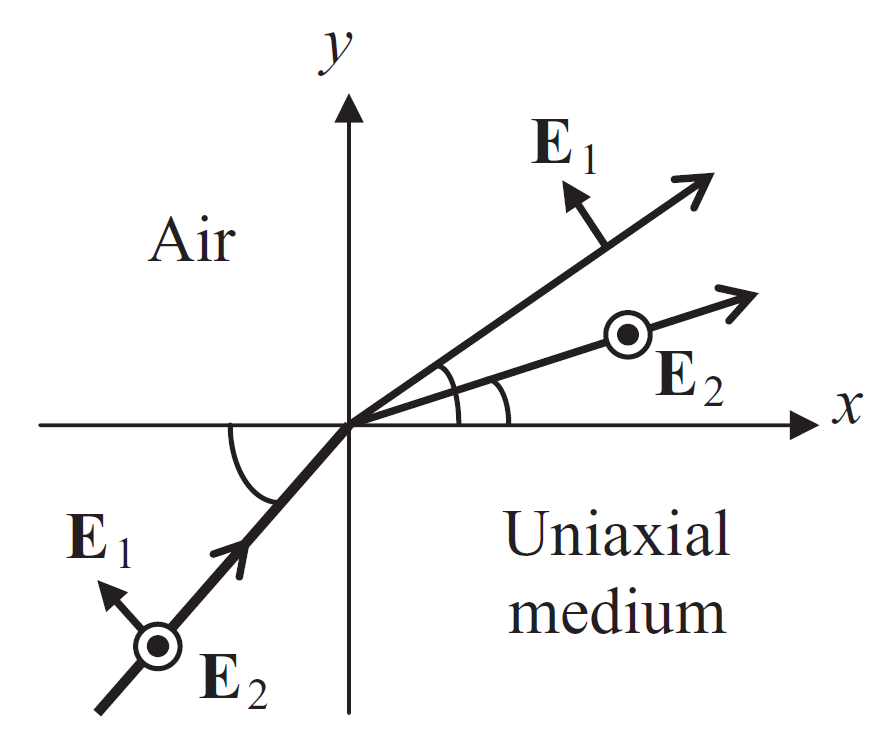
\includegraphics[width=0.3\textwidth]{平面波斜入射到单轴媒质.PNG}
    \caption{平面波斜入射到单轴媒质}
    \label{fig:fig47}
\end{figure}
\\
此时,寻常波电场平行于$xy$平面,波数为$k_0=w\sqrt{\mu\epsilon}$,非寻常波电场沿$z$轴方向,波数为$k_e=w\sqrt{\mu\epsilon_z}$,两种波以不同的相速传播,当具有两种极化的平面波入射到空气和单轴媒质的分界面时,根据极化方式的不同,透射波将分裂成两束沿不同方向传播的平面波。这种现象称为\textbf{\color{blue}{双折射}}。对于广义非寻常波,即使寻常波和非寻常波的传播方向相同,能量传播方向也不同,因此也会呈现双折射现象。\par
如果媒质的$z$方向引入一个电导率,则媒质的介电常数变为:
\begin{align}
    \label{eq:eq481}
    \overline{\vec{\epsilon}}=
        \left[
            \begin{matrix}
                \epsilon & 0 & 0 \\
                0 & \epsilon & 0 \\
                0 & 0 & \epsilon_z-j\sigma_z/w \\
            \end{matrix}
        \right]
\end{align}
对于寻常波,不受电导率影响,其波数仍为$k_0=w\sqrt{\mu\epsilon}$;而对于非寻常波,如果$\sigma_z$很大,则其波数为:
\begin{align}
    \label{eq:eq482}
    k_e=w\sqrt{\mu(\epsilon_z-j\frac{\sigma_z}{w})}\approx\sqrt{\frac{w\mu\sigma_z}{2}}-j\sqrt{\frac{w\mu\sigma_z}{2}}
\end{align}
因此,非寻常波将被衰减。如果衰减跟大,以至于非寻常波可以被忽略,则这样的材料称为偏振片。
\subsubsection{回旋媒质}
考虑媒质的介电常数为:
\begin{align}
    \label{eq:eq483}
    \overline{\vec{\epsilon}}=
        \left[
            \begin{matrix}
                \epsilon & -j\epsilon_g & 0 \\
                j\epsilon_g & \epsilon & 0 \\
                0 & 0 & \epsilon_z \\
            \end{matrix}
        \right]
\end{align}
则根据式\ref{eq:eq456},且假设波矢量位于$xz$平面,即$\vec{\beta}=\hat{x}\beta_x+\hat{z}\beta_z$,则
\begin{align}
    \label{eq:eq484}
    \left[
        \begin{matrix}
            \beta_z^2-w^2\mu\epsilon & jw^2\mu\epsilon_g & -\beta_x\beta_z \\
            -jw^2\mu\epsilon_g & \beta_x^2+\beta_z^2-w^2\mu\epsilon & 0 \\
            -\beta_x\beta_z & 0 & \beta_x^2-w^2\mu\epsilon_z \\
        \end{matrix}
    \right]
    \left[
        \begin{matrix}
            E_x \\
            E_y \\
            E_z \\
        \end{matrix}
    \right]=0
\end{align}
令$\vec{\beta}=\hat{x}\beta\sin\theta+\hat{z}\beta\cos\theta$,$k=w\sqrt{\mu\epsilon}$,$k_z=w\sqrt{\mu\epsilon_z}$,$k_g=w\sqrt{\mu\epsilon_g}$,则上式写成
\begin{align}
    \label{eq:eq485}
    \left[
        \begin{matrix}
            \beta^2\cos^2\theta-k^2 & jk^2_g & -\beta^2\sin\theta\cos\theta \\
            -jk_g & \beta^2-k^2 & 0 \\
            -\beta^2\sin\theta\cos\theta & 0 & \beta^2\sin^2\theta-k_z^2 \\
        \end{matrix}
    \right]
    \left[
        \begin{matrix}
            E_x \\
            E_y \\
            E_z \\
        \end{matrix}
    \right]=0
\end{align}
若方程要有非零解,则
\begin{align}
    \label{eq:eq486}
    &\left|
        \begin{matrix}
            \beta^2\cos^2\theta-k^2 & jk^2_g & -\beta^2\sin\theta\cos\theta \\
            -jk_g & \beta^2-k^2 & 0 \\
            -\beta^2\sin\theta\cos\theta & 0 & \beta^2\sin^2\theta-k_z^2 \\
        \end{matrix}
    \right| \\
    =&(\beta^2-k^2)(k^2k_z^2-k^2\beta^2\sin^2\theta)-k_g^4(\beta^2\sin^2\theta-k_z^2) \\
    =&A\beta^4-B\beta^2+C \\
    =&0
\end{align}
式中,$A=k^2\sin^2\theta+k_z^2\cos^2\theta$,$B=(k^4-k_g^4)\sin^2\theta+k^2k_z^2(1+\cos^2\theta)$,$C=(k^4-k_g^4)k_z^2$。上式的解为
\begin{align}
    \label{eq:eq487}
    \beta^2=\frac{B\pm\sqrt{B^2-4AC}}{2A}
\end{align}
由式\ref{eq:eq485}可得
\begin{align}
    \label{eq:eq488}
    \frac{E_x}{E_y}=\frac{\beta^2-k^2}{jk^2_g} \\
    \label{eq:eq489}
    \frac{E_x}{E_z}=\frac{\beta^2\sin^2\theta-k_z^2}{\beta^2\sin\theta\cos\theta}
\end{align}
因此平面波的电场可以写成:
\begin{align}
    \label{eq:eq490}
    \mathbf{E}=\left(\hat{x}+\hat{y}\frac{jk^2_g}{\beta^2-k^2}+\hat{z}\frac{\beta^2\sin\theta\cos\theta}{\beta^2\sin^2\theta-k_z^2}\right)E_{x0}e^{-j\beta(x\sin\theta+z\cos\theta)}
\end{align}
(1)当波沿$z$轴传播,即$\theta=0$时,式\ref{eq:eq487}写成:
\begin{align}
    \label{eq:eq491}
    \beta^2=\beta_{\pm}^2=k^2\pm k_g^2=w^2\mu(\epsilon\pm\epsilon_g)
\end{align}
式\ref{eq:eq488}、式\ref{eq:eq489}写成:
\begin{align}
    \label{eq:eq492}
    \frac{E_x}{E_y}=\frac{\pm k^2_g}{jk^2_g}=\mp j \\
    \label{eq:eq493}
    E_z=0
\end{align}
式\ref{eq:eq490}描述的电场写成:
\begin{align}
    \label{eq:eq494}
    \mathbf{E}=\left(\hat{x}+j\hat{y}\right)E_{x0}e^{-j\beta_{\pm}}
\end{align}
上式表明,当平面波沿$z$轴传播时,左旋极化分量将以波数$\beta_+=w\sqrt{\mu(\epsilon+\epsilon_g)}$,即相速$v_{p+}=w/\beta_+$传播,而右旋极化分量将以波数$\beta_-=w\sqrt{\mu(\epsilon-\epsilon_g)}$,即相速$v_{p-}=w/\beta_-$传播。考虑一个线极化波,并把它分解成两个圆极化波,即
\begin{align}
    \label{eq:eq495}
    \mathbf{E}=\hat{x}E_0e^{-j\beta z}=\frac{1}{2}(\hat{x}-j\hat{y})E_0e^{-j\beta_- z}+\frac{1}{2}(\hat{x}+j\hat{y})E_0e^{-j\beta_+ z}
\end{align}
在媒质中的$z=d$处,电场为
\begin{align}
    \label{eq:eq496}
    \mathbf{E}&=\frac{1}{2}(\hat{x}-j\hat{y})E_0e^{-j\beta_- d}+\frac{1}{2}(\hat{x}+j\hat{y})E_0e^{-j\beta_+ d} \\
              &=\frac{1}{2}\hat{x}E_0(e^{-j\beta_- d}+e^{-j\beta_+ d})-\frac{1}{2}j\hat{y}E_0(e^{-j\beta_- d}-e^{-j\beta_+ d})
\end{align}
其$x$分量与$y$分量的比值为:
\begin{align}
    \label{eq:eq497}
    \frac{E_x}{E_y}=\frac{\frac{1}{2}E_0(e^{-j\beta_- d}+e^{-j\beta_+ d})}{-\frac{1}{2}jE_0(e^{-j\beta_- d}-e^{-j\beta_+ d})}=\cot\left[\frac{(\beta_+-\beta_-)d}{2}\right]
\end{align}
由此可知,在媒质中的$z=d$处,电磁波仍然是线极化波,只是极化方向与原来的方向相比旋转了一个角度:
\begin{align}
    \label{eq:eq498}
    \theta_F=\frac{(\beta_+-\beta_-)d}{2}
\end{align}
这种现象称为\textbf{\color{blue}{法拉第旋转}}。\\
(2)当波沿$x$轴传播,即$\theta=\pi/2$时,根据式\ref{eq:eq487},当$\beta^2=k_z^2=w^2\mu\epsilon_z$时,电场写成
\begin{align}
    \label{eq:eq499}
    \mathbf{E}=\hat{z}E_0e^{-j\beta x}
\end{align}
此时电场受$\epsilon_z$影响,为非寻常波。当$\beta^2=k^2-\frac{k_g^4}{k^2}=w^2\mu\epsilon-\frac{w^2\mu\epsilon_g^2}{\epsilon}$时,电场写成
\begin{align}
    \label{eq:eq500}
    \mathbf{E}=(\hat{x}-\hat{y}\frac{j\epsilon}{\epsilon_g})E_{x0}e^{-j\beta x}
\end{align}
由上式可知,电场矢量的终端在$xy$平面,即波矢量所在的平面内旋转,轨迹是一个椭圆,也成为椭圆极化。
\subsubsection{手征媒质}
手征媒质是一种双各向同性媒质,其场强与通量密度的关系为:
\begin{align}
    \label{eq:eq501}
    \mathbf{D}=\epsilon\mathbf{E}-j\chi\mathbf{H} \\
    \label{eq:eq502}
    \mathbf{B}=\mu\mathbf{H}+j\chi\mathbf{E}
\end{align}
其中,$\chi$称为\textbf{\color{blue}{手征参量}}。其对应的麦克斯韦方程为
\begin{align}
    \label{eq:eq503}
    \vec{\beta}\times\mathbf{E}=w\mathbf{B} \\
    \label{eq:eq504}
    \vec{\beta}\times\mathbf{H}=-w\mathbf{D} \\
    \label{eq:eq505}
    \vec{\beta}\cdot\mathbf{D}=0 \\
    \label{eq:eq506}
    \vec{\beta}\cdot\mathbf{B}=0
\end{align}
将式\ref{eq:eq501}、式\ref{eq:eq502}代入式\ref{eq:eq503}、式\ref{eq:eq504}中,有
\begin{align}
    \label{eq:eq507}
    \left[
        \begin{matrix}
            \vec{\beta}\times\overline{\mathbf{I}}-jw\chi\overline{\mathbf{I}} & -w\mu\overline{\mathbf{I}} \\
            w\epsilon\overline{\mathbf{I}} & \vec{\beta}\times\overline{\mathbf{I}}-jw\chi\overline{\mathbf{I}} \\
        \end{matrix}
    \right]\cdot
    \left[
        \begin{matrix}
            \mathbf{E} \\
            \mathbf{H} \\
        \end{matrix}
    \right]=0
\end{align}
式中$\mathbf{E}$是单位张量。假设波沿$z$方向传播,因此$D_z=B_z=E_z=H_z=0$,则上式写成
\begin{align}
    \label{eq:eq508}
    \left[
        \begin{matrix}
            -\beta & jw\chi \\
            jw\chi & \beta \\
        \end{matrix}
    \right]
    \left[
        \begin{matrix}
            E_x \\
            E_y \\
        \end{matrix}
    \right]&=-
    \left[
        \begin{matrix}
            0 & w\mu \\
            w\mu & 0 \\
        \end{matrix}
    \right]
    \left[
        \begin{matrix}
            H_x \\
            H_y \\
        \end{matrix}
    \right] \\
    \label{eq:eq509}
    \left[
        \begin{matrix}
            -\beta & jw\chi \\
            jw\chi & \beta \\
        \end{matrix}
    \right]
    \left[
        \begin{matrix}
            H_x \\
            H_y \\
        \end{matrix}
    \right]&=
    \left[
        \begin{matrix}
            0 & w\mu \\
            w\mu & 0 \\
        \end{matrix}
    \right]
    \left[
        \begin{matrix}
            E_x \\
            E_y \\
        \end{matrix}
    \right]
\end{align}
消去磁场,得
\begin{align}
    \label{eq:eq510}
    \left[
        \begin{matrix}
            2jw\chi\beta & \beta^2+w^2\chi^2-w^2\mu\epsilon \\
            \beta^2+w^2\chi^2-w^2\mu\epsilon & -2jw\chi\beta \\
        \end{matrix}
    \right]
    \left[
        \begin{matrix}
            E_x \\
            E_y \\
        \end{matrix}
    \right]=0
\end{align}
若方程要有非零解,则系数矩阵的行列式为零,解得
\begin{align}
    \label{eq:eq511}
    \beta_{\pm}=w\sqrt{\mu\epsilon}\pm w\chi
\end{align}
由式\ref{eq:eq510}得
\begin{align}
    \label{eq:eq512}
    \frac{E_x}{E_y}=\pm j
\end{align}
因此,手征媒质中有两种电磁波可以传播,一种是左旋圆极化波,另一种是右旋圆极化波,其相速分别为:
\begin{align}
    \label{eq:eq513}
    v_{p+}=\frac{w}{\beta_+}=\frac{1}{\sqrt{\mu\epsilon}+\chi} \\
    \label{eq:eq514}
    v_{p-}=\frac{w}{\beta_-}=\frac{1}{\sqrt{\mu\epsilon}-\chi}
\end{align}
任意平面波都可以分解成左旋圆极化波和右旋圆极化波的叠加,因此进入手征媒质后,两种圆极化分量将以不同的相速传播,因此也会发生法拉第旋转和双折射。回旋媒质是非互易的,而手征媒质是互易的。
\section{\textsf{波导}}
\newpage
\section{\textsf{有限差分法}}
\label{sec:sec6}
\subsection{有限差分公式}
有限差分法的基本思想是对偏微分方程中的微分算子进行近似。从求导定义出发,如图\ref{fig:fig48}所示。
\begin{figure}[ht]
    \centering
    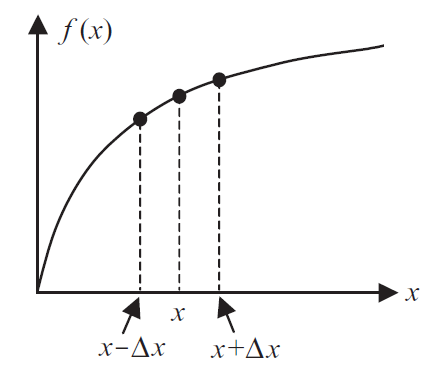
\includegraphics[width=0.3\textwidth]{有限差分近似.PNG}
    \caption{有限差分近似}
    \label{fig:fig48}
\end{figure}
\\
定义\textbf{\color{blue}{前向差分公式}}:
\begin{align}
    \label{eq:eq515}
    f'(x)\approx\frac{f(x+\Delta x)-f(x)}{\Delta x}
\end{align}
定义\textbf{\color{blue}{后向差分公式}}:
\begin{align}
    \label{eq:eq516}
    f'(x)\approx\frac{f(x)-f(x-\Delta x)}{\Delta x}
\end{align}
定义\textbf{\color{blue}{中心差分公式}}:
\begin{align}
    \label{eq:eq517}
    f'(x)\approx\frac{f(x+\Delta x)-f(x-\Delta x)}{2\Delta x}
\end{align}
对于二阶导数,最广泛的应用是先用中心差分求解一阶导数,再对一阶导数使用中心差分,即
\begin{align}
    \label{eq:eq518}
    f''(x)\approx\frac{f'(x+\Delta x/2)-f'(x-\Delta x/2)}{\Delta x}\approx\frac{f(x+\Delta x)-2f(x)+f(x-\Delta x)}{(\Delta x)^2}
\end{align}
根据泰勒级数:
\begin{align}
    \label{eq:eq519}
    f(x+\Delta x)=f(x)+f'(x)\Delta x+\frac{1}{2}f''(x)(\Delta x)^2+\frac{1}{6}f'''(x)(\Delta x)^3+\cdots \\
    \label{eq:eq520}
    f(x-\Delta x)=f(x)-f'(x)\Delta x+\frac{1}{2}f''(x)(\Delta x)^2-\frac{1}{6}f'''(x)(\Delta x)^3+\cdots
\end{align}
分别可得
\begin{align}
    \label{eq:eq521}
    f'(x)=\frac{f(x+\Delta x)-f(x)}{\Delta x}+O(\Delta x)=\frac{f(x)-f(x-\Delta x)}{\Delta x}+O(\Delta x)
\end{align}
其中$O(\Delta x)$表示所有包含$(\Delta x)^p(p\geq1)$的余项之和,与$\Delta x$成正比,因此,前向差分与后向差分具有一阶精度。将式\ref{eq:eq519}、式\ref{eq:eq520}相减,可得
\begin{align}
    \label{eq:eq522}
    f'(x)=\frac{f(x+\Delta x)-f(x-\Delta x)}{2\Delta x}+O[(\Delta x)^2]
\end{align}
因此,中心差分具有二阶精度。将式\ref{eq:eq519}、式\ref{eq:eq520}相加,可得
\begin{align}
    \label{eq:eq523}
    f''(x)=\frac{f(x+\Delta x)-2f(x)+f(x-\Delta x)}{(\Delta x)^2}+O[(\Delta x)^2]
\end{align}
因此,二阶导数的中心差分具有二阶精度。
\subsection{一维分析}
\subsubsection{扩散方程}
从麦克斯韦方程出发:
\begin{align}
    \label{eq:eq524}
    \nabla \times \vec{\mathcal{E}}&=-\mu\frac{\partial \vec{\mathcal{H}}}{\partial t}-\vec{\mathcal{M}}_i \\
    \label{eq:eq525}
    \nabla \times \vec{\mathcal{H}}&=\epsilon\frac{\partial \vec{\mathcal{E}}}{\partial t}+\sigma\vec{\mathcal{E}} +\vec{\mathcal{J}}_{i}
\end{align}
则在导体损耗很大的媒质中,传导电流远大于位移电流,因此,忽略位移电流后吗,电场所满足的二阶偏微分方程为:
\begin{align}
    \label{eq:eq526}
    \nabla \times \nabla \times \vec{\mathcal{E}}=-\mu\sigma\frac{\partial \vec{\mathcal{E}}}{\partial t}-\mu\frac{\partial\vec{\mathcal{J}}_{i}}{\partial t}
\end{align}
假设$\vec{\mathcal{J}}_{i}$和$\vec{\mathcal{E}}$只有$z$方向上的分量,且只在$x$方向上有变化,则上式简化为:
\begin{align}
    \label{eq:eq527}
    \frac{\partial^2 \mathcal{E}_z}{\partial x^2}-\mu\sigma\frac{\partial \mathcal{E}_z}{\partial t}=\mu\frac{\partial\mathcal{J}_{z}}{\partial t}
\end{align}
上式形式的方程称为\textbf{\color{blue}{扩散方程}}。\par
分别离散$x$轴和时间轴,记为$x=i\Delta x$,其中$i=0,1,2,\cdots,M$,$t=n\Delta t$,其中$n=0,1,2,\cdots,N$,则随时间和空间变化的$\mathcal{E}_z(x,t)$写成
\begin{align}
    \label{eq:eq528}
    \mathcal{E}_z(x,t)=\mathcal{E}_z(i\Delta x,n\Delta t)=\mathcal{E}_z^n(i)
\end{align}
对$x$的二阶导数应用中心差分,$t$的一阶导数应用前向差分,可将式\ref{eq:eq527}写成:
\begin{align}
    \label{eq:eq529}
     &\frac{\mathcal{E}_z(x+\Delta x,t)-2\mathcal{E}_z(x,t)+\mathcal{E}_z(x-\Delta x,t)}{(\Delta x)^2}-\mu\sigma\frac{\mathcal{E}_z(x,t+\Delta t)-\mathcal{E}_z(x,t)}{\Delta t} \nonumber \\
    =&\mu\frac{\mathcal{J}_z(x,t+\Delta t)-\mathcal{J}_z(x,t)}{\Delta t} \nonumber \\
    =&\frac{\mathcal{E}_z^n(i+1)-2\mathcal{E}_z^n(i)+\mathcal{E}_z^n(i-1)}{(\Delta x)^2}-\mu\sigma\frac{\mathcal{E}_z^{n+1}(i)-\mathcal{E}_z^n(i)}{\Delta t} \nonumber \\
    =&\mu\frac{\mathcal{J}_z^{n+1}(i)-\mathcal{J}_z^{n}(i)}{\Delta t}
\end{align}
整理后重写为:
\begin{align}
    \label{eq:eq530}
    \mathcal{E}_z^{n+1}(i)=\mathcal{E}_z^{n}(i)+\frac{\Delta t}{\mu\sigma(\Delta x)^2}\left[\mathcal{E}_z^{n}(i+1)-2\mathcal{E}_z^{n}(i)+\mathcal{E}_z^{n}(i-1)\right]-\frac{1}{\sigma}\left[\mathcal{J}_z^{n+1}(i)-\mathcal{E}_z^{n}(i)\right]
\end{align}
上式称为\textbf{\color{blue}{时间步进公式}}。如果已知源的所有值以及场的初始值,则利用时间步进公式,可以得到任意时刻的电场值。上式具有一阶精度。\par
在计算边界点,即$\mathcal{E}_z^{n}(0)$和$\mathcal{E}_z^{n}(M)$时,将需要$\mathcal{E}_z^{n}(-1)$和$\mathcal{E}_z^{n}(M+1)$的值,这些值均在计算区域外且位置,因此要给定边界条件。\textbf{\color{blue}{Dirichlet条件}}直接给定边界处的场值,无需计算,即
\begin{align}
    \label{eq:eq533}
    \mathcal{E}_z(x=0,t)=p(t)
\end{align}
\textbf{\color{blue}{Neumann条件}}规定了边界处的法向导数值,即
\begin{align}
    \label{eq:eq531}
    \left.\frac{\partial \mathcal{E}_z(x,t)}{\partial x}\right|_{x=0}=q(t)
\end{align}
使用中心差分离散,可得
\begin{align}
    \label{eq:eq532}
    \mathcal{E}_z^{n}(-1)=\mathcal{E}_z^{n}(1)-2\Delta xq^n
\end{align}
\subsubsection{波动方程}
根据式\ref{eq:eq524}、式\ref{eq:eq525},当介质无耗时,电场满足的二阶偏微分方程为:
\begin{align}
    \label{eq:eq534}
    \nabla \times \nabla \times \vec{\mathcal{E}}=-\mu\epsilon\frac{\partial^2 \vec{\mathcal{E}}}{\partial t^2}-\mu\frac{\partial\vec{\mathcal{J}}_{i}}{\partial t}
\end{align}
假设$\vec{\mathcal{J}}_{i}$和$\vec{\mathcal{E}}$只有$z$方向上的分量,且只在$x$方向上有变化,则上式简化为:
\begin{align}
    \label{eq:eq535}
    \frac{\partial^2 \mathcal{E}_z}{\partial x^2}-\mu\epsilon\frac{\partial^2 \mathcal{E}_z}{\partial t^2}=\mu\frac{\partial\mathcal{J}_{z}}{\partial t}
\end{align}
上式形式的方程称为\textbf{\color{blue}{波动方程}}。\par
对空间和时间导数应用中心差分,则波动方程重写为:
\begin{align}
    \label{eq:eq536}
     &\frac{\mathcal{E}_z(x+\Delta x,t)-2\mathcal{E}_z(x,t)+\mathcal{E}_z(x-\Delta x,t)}{(\Delta x)^2}-\mu\epsilon\frac{\mathcal{E}_z(x,t+\Delta t)-2\mathcal{E}_z(x,t)+\mathcal{E}_z(x,t-\Delta t)}{(\Delta t)^2} \nonumber \\
    =&\mu\frac{\mathcal{J}_z(x,t+\Delta t)-\mathcal{J}_z(x,t-\Delta t)}{2\Delta t} \nonumber \\
    =&\frac{\mathcal{E}_z^n(i+1)-2\mathcal{E}_z^n(i)+\mathcal{E}_z^n(i-1)}{(\Delta x)^2}-\mu\epsilon\frac{\mathcal{E}_z^{n+1}(i)-2\mathcal{E}_z^n(i)+\mathcal{E}_z^{n-1}(i)}{(\Delta t)^2} \nonumber \\
    =&\mu\frac{\mathcal{J}_z^{n+1}(i)-\mathcal{J}_z^{n-1}(i)}{2\Delta t}
\end{align}
整理上式得到具有二阶精度的时间步进公式:
\begin{align}
    \label{eq:eq537}
    \mathcal{E}_z^{n+1}(i)=&2\mathcal{E}_z^{n}(i)-\mathcal{E}_z^{n-1}(i)+\frac{(\Delta t)^2}{\mu\epsilon(\Delta x)^2}\left[\mathcal{E}_z^n(i+1)-2\mathcal{E}_z^n(i)+\mathcal{E}_z^n(i-1)\right] \nonumber \\
                           &\qquad-\frac{\Delta t}{2\epsilon}\left[\mathcal{J}_z^{n+1}(i)-\mathcal{J}_z^{n-1}(i)\right]
\end{align}
当已知源电流、场的初始值以及边界条件时,可以利用上式计算任意时刻的场值。
\subsubsection{稳定性分析}
通常来说,若关注的最高频率为$f_{max}$,其相应波长为$\lambda_{min}=c/f_{max}$,周期为$T_{min}=1/f_{max}$,则$\Delta x$和$\Delta t$应该满足$\Delta x<\lambda_{min}/20$和$\Delta t<T_{min}/20$。由于场的空间变化和时间变化是相关的,所以$\Delta x$和$\Delta t$的选择不是相互独立的,若选择不恰当,则时间步进过程会不稳定,所计算的场值呈指数增加,或为非物理的解。\\
(1)考虑式\ref{eq:eq530},丢掉源项,此时求解区域的场的能量不应随时间增加。将场展开为傅里叶级数:
\begin{align}
    \label{eq:eq538}
    \mathcal{E}_z^{n}(i)=\sum_{m=-\infty}^{\infty}A_m^ne^{jk_mi\Delta x}\qquad k_m=\frac{m\pi}{L}
\end{align}
其中$L=M\Delta x$表示求解区域的长度。将式\ref{eq:eq538}代入式\ref{eq:eq530}的无源形式,则
\begin{align}
    \label{eq:eq539}
    A_m^{n+1}=(1-2r)A_m^n+r(e^{jk_m\Delta x}+e^{-jk_m\Delta x})A_m^n=\left[1-4r\sin^2\left(\frac{k_m\Delta x}{2}\right)\right]A_m^n
\end{align}
其中$r=\Delta t/\mu\sigma(\Delta x)^2$,定义放大因子$g_m$:
\begin{align}
    \label{eq:eq540}
    g_m=\frac{A_m^{n+1}}{A_m^{n}}=1-4r\sin^2\left(\frac{k_m\Delta x}{2}\right)
\end{align}
由上式知,$1-4r\leq g_m\leq 1$。由于场的能量正比于各傅里叶模式幅度的平方和,为满足场的能量不应随时间增加,$g_m$需满足$|g_m|\leq 1$,因此有$r\leq\frac{1}{2}$,即
\begin{align}
    \label{eq:eq541}
    \Delta t\leq\frac{1}{2}\mu\sigma(\Delta x)^2
\end{align}
在此条件下,场的能量不随$n$的增加而增加,时间步进过程稳定,这个条件称为\textbf{\color{blue}{稳定性条件}},称式\ref{eq:eq530}是\textbf{\color{blue}{有条件稳定}}的。 \\
(2)考虑式\ref{eq:eq537},同样在丢掉源项后求解区域的场的能量不随时间增加。将场展开为式\ref{eq:eq538}所示傅里叶级数,将其代入式\ref{eq:eq537}的无源形式,则
\begin{align}
    \label{eq:eq542}
    A_m^{n+1}=2\left[1-2r\sin^2\left(\frac{k_m\Delta x}{2}\right)\right]A_m^n-A_m^{n-1}
\end{align}
其中$r=(\Delta t)^2/\mu\epsilon(\Delta x)^2$,定义放大因子$g_m$:
\begin{align}
    \label{eq:eq543}
    g_m=\frac{A_m^{n+1}}{A_m^{n}}=\frac{A_m^{n}}{A_m^{n-1}}
\end{align}
则有
\begin{align}
    \label{eq:eq544}
    g_m^2-2\alpha_mg_m+1=0\qquad\alpha_m=1-2r\sin^2\left(\frac{k_m\Delta x}{2}\right)
\end{align}
其解为
\begin{align}
    \label{eq:eq545}
    g_m=\alpha_m\pm\sqrt{\alpha^2_m-1}
\end{align}
由上式知,只有$\alpha^2_m\leq 1$时,$g_m$才满足$|g_m|\leq 1$,因此有$r\leq1$,即
\begin{align}
    \label{eq:eq546}
    \Delta t\leq\Delta x\sqrt{\mu\epsilon}
\end{align}
因此,式\ref{eq:eq537}也是有条件稳定的。\par
如果对式\ref{eq:eq527}中的时间导数使用中心差分近似,以获得二阶精度的时间步进公式,则根据上述分析方法,有
\begin{align}
    \label{eq:eq547}
    g_m^2+2\alpha_mg_m-1=0\qquad\alpha_m=\frac{4\Delta t}{\mu\sigma(\Delta x)^2}\sin^2\left(\frac{k_m\Delta x}{2}\right)
\end{align}
其解为
\begin{align}
    \label{eq:eq548}
    g_m=-\alpha_m\pm\sqrt{\alpha^2_m+1}
\end{align}
无论$\alpha_m$取何值,始终有$|g_m|>1$,因此不稳定。
\subsubsection{数值色散分析}
在使用有限差分法时,由于数值离散,模拟的波速与物理真实的波速值略有不同,这将导致波解的相位出现误差,这种现象称为\textbf{\color{blue}{数值色散}},其造成的误差称为\textbf{\color{blue}{数值相位误差}},数值色散分析给出了有限差分离散中所产生和传播的相位误差。\par
考虑一沿$x$方向传播的平面波:
\begin{align}
    \label{eq:eq549}
    \mathcal{E}_z(x,t)=Re\left[E_0d^{j(wt-kx)}\right]
\end{align}
其中$k=w\sqrt{\mu\epsilon}$,在有限差分网格上,数值离散的波表示为:
\begin{align}
    \label{eq:eq550}
    \mathcal{E}_z^n(i)=Re\left[E_0d^{j(wn\Delta t-\tilde{k}i\Delta x)}\right]
\end{align}
其中$\tilde{k}$表示数值波数。将上式代入式\ref{eq:eq537}的无源形式,得
\begin{align}
    \label{eq:eq551}
    \cos(w\Delta t)=(1-r)+r\cos(\tilde{k}\Delta x)
\end{align}
其中$r=(\Delta t)^2/\mu\epsilon(\Delta x)^2$,解得数值波数为
\begin{align}
    \label{eq:eq552}
    \tilde{k}=\frac{1}{\Delta x}\arccos\left(1-\frac{2}{r}\sin^2\frac{w\Delta t}{2}\right)
\end{align}
用级数展开式的前三项近似式\ref{eq:eq551}中的余弦函数,得
\begin{align}
    \label{eq:eq553}
    k^2-\frac{1}{12}k^2(w\Delta t)^2\approx\tilde{k}^2-\frac{1}{12}\tilde{k}^2(\tilde{k}\Delta x)^2\qquad\longrightarrow\qquad \frac{\tilde{k}-k}{k}\approx\frac{1}{24}\left[(k\Delta x)^2-(w\Delta t)^2\right]
\end{align}
可以看出,当$\Delta t=\Delta x\sqrt{\mu\epsilon}$时,数值波数$\tilde{k}$与真实波数值$k$相等。因此,在一维波传播问题中,总能找到适当的$\Delta t$来消除相位误差。当$\Delta t$为其他值时,两个波数之间存在微小的差别,此时当波在有限差分网格上传播时将产生相位误差吗,随着传播距离的延长,这个误差逐渐累积,导致数值解完全失真。此误差随着$\Delta x/\lambda$二次衰减\footnote{取$\Delta t=0.5\Delta x\sqrt{\mu\epsilon}$,代入式\ref{eq:eq553}即可得到此结论。},即二次收敛,可以通过减小$\Delta x$有效控制。
\subsection{二维分析}
\subsubsection{时域分析}
根据式\ref{eq:eq524}、式\ref{eq:eq525},当介质无耗时,电场满足的二阶偏微分方程为:
\begin{align}
    \label{eq:eq554}
    \nabla \times \nabla \times \vec{\mathcal{E}}=-\mu\epsilon\frac{\partial^2 \vec{\mathcal{E}}}{\partial t^2}-\mu\sigma\frac{\partial \vec{\mathcal{E}}}{\partial t}-\mu\frac{\partial\vec{\mathcal{J}}_{i}}{\partial t}
\end{align}
假设$\vec{\mathcal{J}}_{i}$和$\vec{\mathcal{E}}$只有$z$方向上的分量,且源和媒质沿$z$轴是均匀的,因此源所产生的场在$z$方向上没有变化,则上式简化为:
\begin{align}
    \label{eq:eq555}
    \frac{\partial^2 \mathcal{E}_z}{\partial x^2}+\frac{\partial^2 \mathcal{E}_z}{\partial y^2}-\mu\epsilon\frac{\partial^2 \mathcal{E}_z}{\partial t^2}-\mu\sigma\frac{\partial\mathcal{E}_z}{\partial t}=\mu\frac{\partial\mathcal{J}_{z}}{\partial t}
\end{align}
用矩形框包围求解区域,再将其划分为$\Delta x\times\Delta y$的小矩形,用$(i,j)$来表示对应的网格点。对上式使用中心差分,得
\begin{align}
    \label{eq:eq556}
    &\frac{\mathcal{E}_z^{n}(i+1,j)-2\mathcal{E}_z^{n}(i,j)+\mathcal{E}_z^{n}(i-1,j)}{(\Delta x)^2}+\frac{\mathcal{E}_z^{n}(i,j+1)-2\mathcal{E}_z^{n}(i,j)+\mathcal{E}_z^{n}(i,j-1)}{(\Delta y)^2} \nonumber \\
    &\qquad-\mu\epsilon_{ij}\frac{\mathcal{E}_z^{n+1}(i,j)-2\mathcal{E}_z^{n}(i,j)+\mathcal{E}_z^{n-1}(i,j)}{(\Delta t)^2}-\mu\sigma_{ij}\frac{\mathcal{E}_z^{n+1}(i,j)-\mathcal{E}_z^{n-1}(i,j)}{2\Delta t} \nonumber \\
    =&\mu\frac{\mathcal{J}_z^{n+1}(i,j)-\mathcal{J}_z^{n-1}(i,j)}{2\Delta t}
\end{align}
其中$\epsilon_{ij}$和$\sigma_{ij}$表示网格点$(i,j)$处的$\epsilon$和$\sigma$,假设$\mu$为常数,则可得时间步进公式:
\begin{align}
    \label{eq:eq557}
    \mathcal{E}_z^{n+1}(i,j)&=\left[\frac{\mu\sigma_{ij}}{2\Delta t}+\frac{\mu\epsilon_{ij}}{(\Delta t)^2}\right]^{-1}\left\{2\mathcal{E}_z^{n}(i,j)\left[\frac{\mu\epsilon_{ij}}{(\Delta t)^2}-\frac{1}{(\Delta x)^2}-\frac{1}{(\Delta y)^2}\right]\right. \nonumber \\
                            &\qquad+\mathcal{E}_z^{n-1}(i,j)\left[\frac{\mu\sigma_{ij}}{2\Delta t}-\frac{\mu\epsilon_{ij}}{(\Delta t)^2}\right]+\frac{1}{(\Delta x)^2}\left[\mathcal{E}_z^{n}(i+1,j)+\mathcal{E}_z^{n}(i-1,j)\right] \nonumber \\
                            &\qquad\left.+\frac{1}{(\Delta y)^2}\left[\mathcal{E}_z^{n}(i,j+1)+\mathcal{E}_z^{n}(i,j-1)\right]-\frac{\mu}{2\Delta t}\left[\mathcal{J}_z^{n+1}(i,j)-\mathcal{J}_z^{n-1}(i,j)\right]\right\}
\end{align}
根据源、初始条件、边界条件的信息,可利用上式计算出任意时刻每个网格点的场。对上式进行稳定性分析,可得稳定性条件为:
\begin{align}
    \label{eq:eq558}
    \Delta t\leq\frac{\sqrt{\mu\epsilon}}{\sqrt{\frac{1}{(\Delta x)^2}+\frac{1}{(\Delta y)^2}}}
\end{align}
通过数值色散分析,可得
\begin{align}
    \label{eq:eq559}
    \left[\frac{1}{c\Delta t}\sin\frac{w\Delta t}{2}\right]^2=\left[\frac{1}{\Delta x}\sin\frac{\tilde{k}_x\Delta x}{2}\right]^2+\left[\frac{1}{\Delta y}\sin\frac{\tilde{k}_y\Delta y}{2}\right]^2
\end{align}
上式可近似得到
\begin{align}
    \label{eq:eq560}
    \frac{\tilde{k}-k}{k}\approx\frac{1}{24}\left[(k\Delta x)^2\cos^4\phi^i+(k\Delta y)^2\sin^4\phi^i-(w\Delta t)^2\right]
\end{align}
其中$\phi^i$是传播方向与$x$轴的夹角,与以为情况不同,没有一个$\Delta t$的选择能消除所有方向的数值色散误差。
\subsubsection{频域分析}
式\ref{eq:eq555}对应的频域表达式为:
\begin{align}
    \label{eq:eq561}
    \frac{\partial^2 {E}_z}{\partial x^2}+\frac{\partial^2 {E}_z}{\partial y^2}+k^2\epsilon_cE_z=g
\end{align}
其中$\epsilon_c=1-j\sigma/w\epsilon$,$g=jw\mu{J}_{z}$,使用中心差分,得
\begin{align}
    \label{eq:eq562}
    &\frac{E_z(i+1,j)-2E_z(i,j)+E_z(i-1,j)}{(\Delta x)^2}+\frac{E_z(i,j+1)-2E_z(i,j)+E_z(i,j-1)}{(\Delta y)^2} \nonumber \\
    &\qquad+k^2\epsilon_{c,ij}E_z(i,j)=g(i,j)
\end{align}
对于每一个网格点,其场值均可以采用上式表示,由此得到一组线性方程组,在给定边界条件下同时求解整个线性方程组,即可求得网格点得场值。线性方程组有两种求解方法:\\
(1)高斯消元法:方程组的稀疏矩阵稀疏,每行最多有5个非零项,可以使用稀疏矩阵求解方法; \\
(2)迭代法:首先将所有$E_z(i,j)$设为零,根据式\ref{eq:eq562}计算一组新的值,重复计算式\ref{eq:eq562},直到结果收敛。
\subsection{Yee网格}
使用上节描述的有限差分法时会遇到问题,这些问题原子传统的有限差分法在网格点的采样:\\
(1)当网格点位于两种不同媒质的分界面上时,为了保证切向场的连续和法向场的不连续,需要进行相对繁琐的处理;\\
(2)当一个网格点位于导体或媒质的边缘或拐角时,这一点的法向没有明确的定义,其场分量可能无限大,即奇异,因此这个网格点处的场值无法精确描述。
\subsubsection{二维分析}
假设$\vec{\mathcal{J}}_{i}$和$\vec{\mathcal{E}}$只有$z$方向上的分量,且源和媒质沿$z$轴是均匀的,因此源所产生的场在$z$方向上没有变化,为求解$(\mathcal{E}_z,\mathcal{H}_x,\mathcal{H}_y)$,将其麦克斯韦方程组简化为:
\begin{align}
    \label{eq:eq563}
    \frac{\partial\mathcal{E}_z}{\partial y}&=-\mu\frac{\partial\mathcal{H}_x}{\partial t} \\
    \label{eq:eq564}
    \frac{\partial\mathcal{E}_z}{\partial x}&=\mu\frac{\partial\mathcal{H}_y}{\partial t} \\
    \label{eq:eq565}
    \frac{\partial\mathcal{H}_y}{\partial x}-\frac{\partial\mathcal{H}_x}{\partial y}&=\epsilon\frac{\partial\mathcal{E}_z}{\partial t}+\sigma\mathcal{E}_z+\mathcal{J}_z
\end{align}
用一个矩形区域包围求解区域,把区域均匀离散成许多小矩形单元,每个单元的中心点用$(i,j)$表示,在中心点上采样$\mathcal{E}_z$,磁场分量沿着矩形单元的边缘采样,如图\ref{fig:fig49}所示。
\begin{figure}[ht]
    \centering
    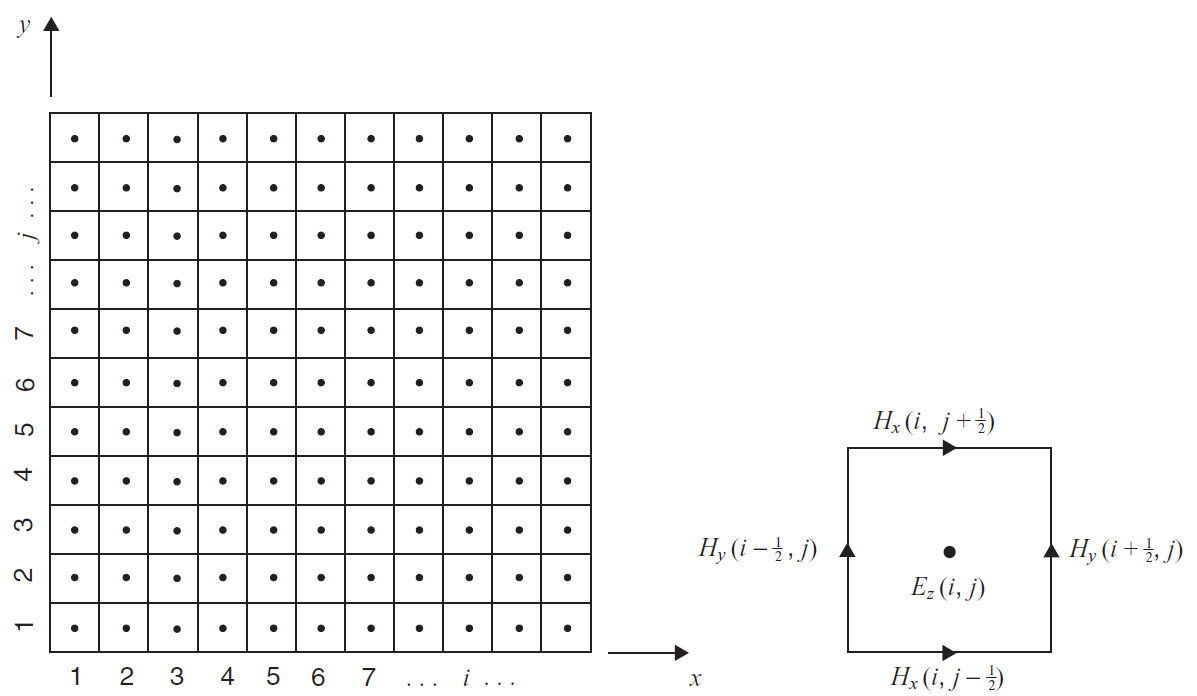
\includegraphics[width=0.8\textwidth]{Yee网格有限差分算法.PNG}
    \caption{Yee网格有限差分算法}
    \label{fig:fig49}
\end{figure}
\par
在$t=n\Delta t$时刻采样电场,在$t=(n+\frac{1}{2})\Delta t$时刻采样磁场,这种采样方式保证了场的唯一定义,并且自动确保了切向场的连续性。对麦克斯韦方程组使用中心差分,可得称为\textbf{\color{blue}{蛙跳时间积分}}的时间步进公式:
\begin{align}
    \label{eq:eq566}
    \mathcal{H}_x^{n+1/2}\left(i,j+\frac{1}{2}\right)&=\mathcal{H}_x^{n-1/2}\left(i,j+\frac{1}{2}\right)-\frac{\Delta}{\mu\Delta y}\left[\mathcal{E}_z^{n}\left(i,j+1\right)-\mathcal{E}_z^{n}\left(i,j\right)\right] \\
    \label{eq:eq567}
    \mathcal{H}_y^{n+1/2}\left(i+\frac{1}{2},j\right)&=\mathcal{H}_y^{n-1/2}\left(i+\frac{1}{2},j\right)+\frac{\Delta}{\mu\Delta x}\left[\mathcal{E}_z^{n}\left(i+1,j\right)-\mathcal{E}_z^{n}\left(i,j\right)\right] \\
    \label{eq:eq568}
    \mathcal{E}_z^{n+1}\left(i,j\right)&=\frac{1}{\beta(i,j)}\left\{\alpha(i,j)\mathcal{E}_z^{n}\left(i,j\right)+\frac{1}{\Delta x}\left[\mathcal{H}_y^{n+1/2}\left(i+\frac{1}{2},j\right)-\mathcal{H}_y^{n+1/2}\left(i-\frac{1}{2},j\right)\right]\right. \nonumber \\
                                       &\qquad\left.-\frac{1}{\Delta y}\left[\mathcal{H}_x^{n+1/2}\left(i,j+\frac{1}{2}\right)-\mathcal{H}_x^{n+1/2}\left(i,j-\frac{1}{2}\right)\right]-\mathcal{J}_z^{n+1/2}(i,j)\right\}
\end{align}
其中,
\begin{align}
    \label{eq:eq569}
    \alpha=\frac{\epsilon}{\Delta t}-\frac{\sigma}{2}\qquad\beta=\frac{\epsilon}{\Delta t}+\frac{\sigma}{2}
\end{align}
若给定$(\mathcal{E}_z,\mathcal{H}_x,\mathcal{H}_y)$的初始值以及边界条件,则可以先用式\ref{eq:eq566}、式\ref{eq:eq567}计算磁场,然后用式\ref{eq:eq568}计算电场。其稳定性条件同式\ref{eq:eq558},色散误差同式\ref{eq:eq560}。
\subsubsection{三维分析}
考虑时域麦克斯韦方程组:
\begin{align}
    \label{eq:eq583}
    \nabla \times \vec{\mathcal{E}}&=-\mu\frac{\partial \vec{\mathcal{H}}}{\partial t} \\
    \label{eq:eq570}
    \nabla \times \vec{\mathcal{H}}&=\epsilon\frac{\partial \vec{\mathcal{E}}}{\partial t}+\sigma\vec{\mathcal{E}} +\vec{\mathcal{J}}_{i}
\end{align}
重写为标量方程:
\begin{align}
    \label{eq:eq571}
    \frac{\partial \mathcal{E}_z}{\partial y}-\frac{\partial \mathcal{E}_y}{\partial z}&=-\mu\frac{\partial \mathcal{H}_x}{\partial t} \\
    \label{eq:eq572}
    \frac{\partial \mathcal{E}_x}{\partial z}-\frac{\partial \mathcal{E}_z}{\partial x}&=-\mu\frac{\partial \mathcal{H}_y}{\partial t} \\
    \label{eq:eq573}
    \frac{\partial \mathcal{E}_y}{\partial x}-\frac{\partial \mathcal{E}_x}{\partial y}&=-\mu\frac{\partial \mathcal{H}_z}{\partial t} \\
    \label{eq:eq574}
    \frac{\partial \mathcal{H}_z}{\partial y}-\frac{\partial \mathcal{H}_y}{\partial z}&=\epsilon\frac{\partial \mathcal{E}_x}{\partial t}+\sigma\mathcal{E}_x+\mathcal{J}_x \\
    \label{eq:eq575}
    \frac{\partial \mathcal{H}_x}{\partial z}-\frac{\partial \mathcal{H}_z}{\partial x}&=\epsilon\frac{\partial \mathcal{E}_y}{\partial t}+\sigma\mathcal{E}_y+\mathcal{J}_y \\
    \label{eq:eq576}
    \frac{\partial \mathcal{H}_y}{\partial x}-\frac{\partial \mathcal{H}_x}{\partial y}&=\epsilon\frac{\partial \mathcal{E}_z}{\partial t}+\sigma\mathcal{E}_z+\mathcal{J}_z
\end{align}
类比二维分析,用一个立方体区域包围求解区域,把区域均匀离散成许多小立方体单元,每个单元的中心点用$(i,j,k)$表示,在单元每条边的中心位置对电场分量采样,在单元每个面的中心位置对磁场分量采样,如图\ref{fig:fig50}所示。
\begin{figure}[ht]
    \centering
    \includegraphics[width=0.4\textwidth]{网格单元上场分量的采样.PNG}
    \caption{网格单元上场分量的采样}
    \label{fig:fig50}
\end{figure}
\par
将整个网格在每个方向上偏移半个单元,则磁场分量的采样点将在单元每条边的中心,电场分量的采样点将在单元每个面的中心。对式\ref{eq:eq571}至式\ref{eq:eq576}使用中心差分,得磁场的时间步进公式:
\begin{align}
    \label{eq:eq577}
    \mathcal{H}_x^{n+1/2}\left(i,j+\frac{1}{2},k+\frac{1}{2}\right)&=\mathcal{H}_x^{n-1/2}\left(i,j+\frac{1}{2},k+\frac{1}{2}\right) \nonumber \\
                                                                   &\qquad-\frac{\Delta t}{\mu \Delta y}\left[\mathcal{E}_z^{n}\left(i,j+1,k+\frac{1}{2}\right)-\mathcal{E}_z^{n}\left(i,j,k+\frac{1}{2}\right)\right] \nonumber \\
                                                                   &\qquad+\frac{\Delta t}{\mu \Delta z}\left[\mathcal{E}_y^{n}\left(i,j+\frac{1}{2},k+1\right)-\mathcal{E}_y^{n}\left(i,j+\frac{1}{2},k\right)\right] \\
    \label{eq:eq578}
    \mathcal{H}_y^{n+1/2}\left(i+\frac{1}{2},j,k+\frac{1}{2}\right)&=\mathcal{H}_y^{n-1/2}\left(i+\frac{1}{2},j,k+\frac{1}{2}\right) \nonumber \\
                                                                   &\qquad-\frac{\Delta t}{\mu \Delta z}\left[\mathcal{E}_x^{n}\left(i+\frac{1}{2},j,k+1\right)-\mathcal{E}_x^{n}\left(i+\frac{1}{2},j,k\right)\right] \nonumber \\
                                                                   &\qquad+\frac{\Delta t}{\mu \Delta x}\left[\mathcal{E}_z^{n}\left(i+1,j,k+\frac{1}{2}\right)-\mathcal{E}_z^{n}\left(i,j,k+\frac{1}{2}\right)\right] \\
    \label{eq:eq579}
    \mathcal{H}_z^{n+1/2}\left(i+\frac{1}{2},j+\frac{1}{2},k\right)&=\mathcal{H}_z^{n-1/2}\left(i+\frac{1}{2},j+\frac{1}{2},k\right) \nonumber \\
                                                                   &\qquad-\frac{\Delta t}{\mu \Delta x}\left[\mathcal{E}_y^{n}\left(i+1,j+\frac{1}{2},k\right)-\mathcal{E}_y^{n}\left(i,j+\frac{1}{2},k\right)\right] \nonumber \\
                                                                   &\qquad+\frac{\Delta t}{\mu \Delta y}\left[\mathcal{E}_x^{n}\left(i+\frac{1}{2},j+1,k\right)-\mathcal{E}_x^{n}\left(i+\frac{1}{2},j,k\right)\right]
\end{align}
电场的时间步进公式:
\begin{align}
    \label{eq:eq580}
    \mathcal{E}_x^{n+1}\left(i+\frac{1}{2},j,k\right)&=\frac{1}{\beta\left(i+\frac{1}{2},j,k\right)}\left\{\alpha\left(i+\frac{1}{2},j,k\right)\mathcal{E}_x^{n}\left(i+\frac{1}{2},j,k\right)\right. \nonumber \\
                                                     &\qquad+\frac{1}{\Delta y}\left[\mathcal{H}_z^{n+1/2}\left(i+\frac{1}{2},j+\frac{1}{2},k\right)-\mathcal{H}_z^{n+1/2}\left(i+\frac{1}{2},j-\frac{1}{2},k\right)\right] \nonumber \\
                                                     &\qquad-\frac{1}{\Delta z}\left[\mathcal{H}_y^{n+1/2}\left(i+\frac{1}{2},j,k+\frac{1}{2}\right)-\mathcal{H}_y^{n+1/2}\left(i+\frac{1}{2},j,k-\frac{1}{2}\right)\right] \nonumber \\
                                                     &\qquad\left.-\mathcal{J}_x^{n+1/2}\left(i+\frac{1}{2},j,k\right)\right\} \\
    \label{eq:eq581}
    \mathcal{E}_y^{n+1}\left(i,j+\frac{1}{2},k\right)&=\frac{1}{\beta\left(i,j+\frac{1}{2},k\right)}\left\{\alpha\left(i,j+\frac{1}{2},k\right)\mathcal{E}_y^{n}\left(i,j+\frac{1}{2},k\right)\right. \nonumber \\
                                                     &\qquad+\frac{1}{\Delta z}\left[\mathcal{H}_x^{n+1/2}\left(i,j+\frac{1}{2},k+\frac{1}{2}\right)-\mathcal{H}_x^{n+1/2}\left(i,j+\frac{1}{2},k-\frac{1}{2}\right)\right] \nonumber \\
                                                     &\qquad-\frac{1}{\Delta x}\left[\mathcal{H}_z^{n+1/2}\left(i+\frac{1}{2},j+\frac{1}{2},k\right)-\mathcal{H}_z^{n+1/2}\left(i-\frac{1}{2},j+\frac{1}{2},k\right)\right] \nonumber \\
                                                     &\qquad\left.-\mathcal{J}_y^{n+1/2}\left(i,j+\frac{1}{2},k\right)\right\} \\
    \label{eq:eq582}
    \mathcal{E}_y^{n+1}\left(i,j,k+\frac{1}{2}\right)&=\frac{1}{\beta\left(i,j,k+\frac{1}{2}\right)}\left\{\alpha\left(i,j,k+\frac{1}{2}\right)\mathcal{E}_z^{n}\left(i,j,k+\frac{1}{2}\right)\right. \nonumber \\
                                                     &\qquad+\frac{1}{\Delta x}\left[\mathcal{H}_y^{n+1/2}\left(i+\frac{1}{2},j,k+\frac{1}{2}\right)-\mathcal{H}_y^{n+1/2}\left(i-\frac{1}{2},j,k+\frac{1}{2}\right)\right] \nonumber \\
                                                     &\qquad-\frac{1}{\Delta y}\left[\mathcal{H}_x^{n+1/2}\left(i,j+\frac{1}{2},k+\frac{1}{2}\right)-\mathcal{H}_x^{n+1/2}\left(i,j-\frac{1}{2},k+\frac{1}{2}\right)\right] \nonumber \\
                                                     &\qquad\left.-\mathcal{J}_z^{n+1/2}\left(i,j,k+\frac{1}{2}\right)\right\}
\end{align}
式中,$\alpha$与$\beta$的定义同式\ref{eq:eq569}。给定源电流、电场和磁场的初始值及边界条件,即可利用以上公式计算各个时刻的电场和磁场。其对于单元尺寸和时间步长具有二阶精度,稳定性条件为:
\begin{align}
    \label{eq:eq584}
    \Delta t\leq\frac{\sqrt{\mu\epsilon}}{\sqrt{\frac{1}{(\Delta x)^2}+\frac{1}{(\Delta y)^2}+\frac{1}{(\Delta z)^2}}}
\end{align}
数值色散公式为:
\begin{align}
    \label{eq:eq585}
    \frac{\tilde{k}-k}{k}\approx\frac{1}{24}\left\{\left[(k\Delta x)^2\cos^4\phi^i+(k\Delta y)^2\sin^4\phi^i\right]\sin^4\theta^i+(k\Delta z)^2\cos^4\theta^i-(w\Delta t)^2\right\}
\end{align}
其中$(\phi^i,\theta^i)$表示波的传播方向。
\subsection{吸收边界条件}
使用有限差分法求解无界电磁问题时,需要将无限空间截断成有限空间,一般引入一个人工表面包围感兴趣的计算区域,该表面应该尽可能地吸收入射到该表面的波,减少反射。常用的两种方法是数学上推导的吸收边界条件和使用人为构造的吸收材料层。
\subsubsection{一维吸收边界条件}
考虑式\ref{eq:eq535}表示的一维波动方程,假设求解区域为$(-\infty<x<\infty)$,源只在有限区域$(a\leq x\leq b)$内存在,其在$x>b$区域产生沿$x$正方向传播的波,在$x<a$区域产生沿$x$负方向传播的波。现将求解区域截断为有限区域$[A,B]$,其中$A<a$,$B>b$,建立一个边界条件,使得波能透过$x=B$和$x=A$且不产生反射。
以$x=B$为例,在这里波沿$x$正方向传播,表示为
\begin{align}
    \label{eq:eq586}
    E_z(x)=E_0e^{-jkx}
\end{align}
其中$E_0$为未知量,$k=w\sqrt{\mu\epsilon}$,将上式对$x$求导,得
\begin{align}
    \label{eq:eq587}
    \frac{\partial E_z}{\partial x}=-jkE_0e^{-jkx}=-jkE_z(x)=-\frac{jw}{c}E_z(x)
\end{align}
上式将场的法向导数与场值本身关联,称为\textbf{\color{blue}{第三类边界条件}},其在时域的表达式为:
\begin{align}
    \label{eq:eq588}
    \frac{\partial \mathcal{E}_z(x,t)}{\partial x}=-\frac{1}{c}\frac{\partial \mathcal{E}_z(x,t)}{\partial t}
\end{align}
将此边界条件应用于$x=B$,波将穿过截断面而不反射。这样的边界条件称为\textbf{\color{blue}{吸收边界条件(ABC)}}。在$x=B$处离散上式,使用后向差分离散对$x$的导数,使用前向差分离散对$t$的导数,得时间步进公式:
\begin{align}
    \label{eq:eq589}
    \mathcal{E}_z^{n+1}(M)=\mathcal{E}_z^{n}(M)-\frac{c\Delta t}{\Delta x}[\mathcal{E}_z^{n}(M)-\mathcal{E}_z^{n}(M-1)]
\end{align}
上式只有一阶精度,其稳定条件为$\Delta t\leq\Delta x/c$,当$\Delta t=\Delta x/c$时,有$\mathcal{E}_z^{n+1}(M)=\mathcal{E}_z^{n}(M-1)$。另一种离散方法是在$x=\left(M-\frac{1}{2}\right)\Delta x$和$t=\left(n+\frac{1}{2}\right)\Delta t$处采用中心差分,得时间步进公式:
\begin{align}
    \label{eq:eq599}
    \mathcal{E}_z^{n+1}(M)=\mathcal{E}_z^{n}(M-1)-\frac{\Delta x-c\Delta t}{\Delta x+c\Delta t}[\mathcal{E}_z^{n}(M)-\mathcal{E}_z^{n+1}(M-1)]
\end{align}
上式具有二阶精度,是无条件稳定的,同样,当$\Delta t=\Delta x/c$时,有$\mathcal{E}_z^{n+1}(M)=\mathcal{E}_z^{n}(M-1)$。
\subsubsection{二维吸收边界条件}
考虑沿$y$轴方向得边界上,有一个平面波入射到此边界,如图\ref{fig:fig51}所示。
\begin{figure}[ht]
    \centering
    \includegraphics[width=0.3\textwidth]{平面波入射到yz平面.PNG}
    \caption{平面波入射到$yz$平面}
    \label{fig:fig51}
\end{figure}
\\
若此边界完全透明,则波继续向前传播且不反射。此时,波表示为:
\begin{align}
    \label{eq:eq590}
    \varphi(x,y)=Ae^{-j(k_xx+k_yy)}
\end{align}
其中$A$为未知量,$k_x=k\cos\theta$,$k_y=k\sin\theta$,将上式对$x$求偏导,得
\begin{align}
    \label{eq:eq591}
    \frac{\partial \varphi}{\partial x}=-jk_xAe^{-j(k_xx+k_yy)}=-jk_x\varphi(x,y)=-jk\cos\theta\varphi(x,y)
\end{align}
此边界条件可以完全吸收与$x$轴成$\theta$角入射的平面波。令$\theta=0$,则有
\begin{align}
    \label{eq:eq592}
    \frac{\partial \varphi}{\partial x}=-jk\varphi(x,y)
\end{align}
称为\textbf{\color{blue}{一阶吸收边界条件}},该边界条件仅吸收与$x$轴平行传播的波,对于其他角度$\theta$,其反射系数为
\begin{align}
    \label{eq:eq593}
    R=\frac{\cos\theta-1}{\cos\theta+1}
\end{align}
显然,当$\theta=0$时,反射系数为零。\par
对于一般的二维问题,不存在完全精确的吸收边界。为改善其精确度,重写式\ref{eq:eq591}为:
\begin{align}
    \label{eq:eq594}
    \frac{\partial \varphi}{\partial x}=-jk_x\varphi&=-j\sqrt{k^2-k_y^2}\varphi=-jk\sqrt{1-\left(\frac{k_y}{k}\right)^2}\varphi \nonumber \\
    &\approx-jk\left[1-\frac{1}{2}\left(\frac{k_y}{k}\right)^2\right]\varphi=-jk\varphi+\frac{j}{2k}k_y^2\varphi=-jk\varphi-\frac{j}{2k}\frac{\partial^2\varphi}{\partial y^2}
\end{align}
上式推导过程中利用了平方根的泰勒展开,保留前两项,以及$\frac{\partial^2\varphi}{\partial y^2}=-k_y^2\varphi$,称为\textbf{\color{blue}{二阶吸收边界条件}}。其对应的反射系数为:
\begin{align}
    \label{eq:eq595}
    R=\frac{\cos\theta+\frac{1}{2}\sin^2\theta-1}{\cos\theta-\frac{1}{2}\sin^2\theta+1}
\end{align}
相比于一阶吸收边界条件,当$\theta=0$时,反射系数为零,$\theta\neq0$时,反射系数更小。将式\ref{eq:eq594}变换到时域:
\begin{align}
    \label{eq:eq596}
    \frac{\partial^2 \varphi}{\partial t\partial x}\approx-\frac{1}{c}\frac{\partial^2 \varphi}{\partial t^2}+\frac{c}{2}\frac{\partial^2 \varphi}{\partial y^2}
\end{align}
称为\textbf{\color{blue}{Engquist-Majda吸收边界条件}}。将上式左边离散为:
\begin{align}
    \label{eq:eq597}
    \frac{\partial^2 \varphi}{\partial t\partial x}&=\frac{\partial}{\partial t}\frac{\varphi(M,j)-\varphi(M-1,j)}{\Delta x} \nonumber \\
                                                   &=\frac{[\varphi^{n+1}(M,j)-\varphi^{n+1}(M-1,j)]-[\varphi^{n}(M,j)-\varphi^{n}(M-1,j)]}{\Delta x\Delta t}
\end{align}
右边使用中心差分,可得时间步进公式:
\begin{align}
    \label{eq:eq598}
    \varphi^{n+1}(M,j)&=\left[\frac{1}{\Delta x\Delta t}+\frac{1}{c(\Delta t)^2}\right]^{-1}\left\{\frac{1}{\Delta x\Delta t}\left[\varphi^{n+1}(M-1,j)-\varphi^{n}(M-1,j)\right]\right. \nonumber \\
                      &\qquad+\left[\frac{1}{\Delta x\Delta t}+\frac{2}{c(\Delta t)^2}-\frac{c}{(\Delta y)^2}\right]\varphi^{n}(M,j)-\frac{1}{c(\Delta t)^2}\varphi^{n-1}(M,j) \nonumber \\
                      &\qquad\left.+\frac{c}{2(\Delta y)^2}\left[\varphi^{n}(M,j-1)+\varphi^{n}(M,j+1)\right]\right\}
\end{align}
上式用于计算吸收边界上的场。
\subsubsection{理想匹配层(PML)}
考虑无源情况下的基于拉伸坐标系的修正麦克斯韦方程组:
\begin{align}
    \label{eq:eq600}
    \nabla_s \times \mathbf{E}&=-jw\mu\mathbf{H} \\
    \label{eq:eq601}
    \nabla_s \times \mathbf{H}&=jw\epsilon\mathbf{E} \\
    \label{eq:eq602}
    \nabla_s \cdot (\epsilon\mathbf{E})&=0 \\
    \label{eq:eq603}
    \nabla_s \cdot (\mu\mathbf{H})&=0
\end{align}
其中,
\begin{align}
    \label{eq:eq604}
    \nabla_s=\hat{x}\frac{1}{s_x}\frac{\partial}{\partial x}+\hat{y}\frac{1}{s_y}\frac{\partial}{\partial y}+\hat{z}\frac{1}{s_z}\frac{\partial}{\partial z}
\end{align}
$s_x$、$s_y$、$s_z$是常数,或分别为$x$、$y$、$z$的函数。考虑一个电磁波,其电场和磁场分别为:
\begin{align}
    \label{eq:eq605}
    \mathbf{E}&=\mathbf{E}_0e^{-j\vec{k}\cdot\vec{r}}=\mathbf{E}_0e^{-j(k_xx+k_yy+k_zz)} \\
    \label{eq:eq606}
    \mathbf{H}&=\mathbf{H}_0e^{-j\vec{k}\cdot\vec{r}}=\mathbf{H}_0e^{-j(k_xx+k_yy+k_zz)}
\end{align}
代入修正麦克斯韦方程组,得
\begin{align}
    \label{eq:eq607}
    \vec{k}_s \times \mathbf{E}&=w\mu\mathbf{H} \\
    \label{eq:eq608}
    \vec{k}_s \times \mathbf{H}&=-w\epsilon\mathbf{E} \\
    \label{eq:eq609}
    \vec{k}_s \cdot (\epsilon\mathbf{E})&=0 \\
    \label{eq:eq610}
    \vec{k}_s \cdot (\mu\mathbf{H})&=0
\end{align}
由上可得
\begin{align}
    \label{eq:eq611}
    \vec{k}_s \times(\vec{k}_s \times \mathbf{E})&=w\mu\vec{k}_s \times \mathbf{H}=-w^2\mu\epsilon \nonumber \\
                                                 &=\vec{k}_s(\vec{k}_s\cdot\mathbf{E})-(\vec{k}_s\cdot\vec{k}_s)\mathbf{E}=-(\vec{k}_s\cdot\vec{k}_s)\mathbf{E}
\end{align}
因此有
\begin{align}
    \label{eq:eq612}
    \vec{k}_s\cdot\vec{k}_s=\left(\frac{k_x}{s_x}\right)^2+\left(\frac{k_y}{s_y}\right)^2+\left(\frac{k_z}{s_z}\right)^2=w^2\mu\epsilon=k^2
\end{align}
其解为:
\begin{align}
    \label{eq:eq613}
    k_x=ks_x\sin\theta\cos\phi\qquad k_y=ks_y\sin\theta\sin\phi\qquad k_z=ks_z\cos\theta
\end{align}
平面波的波阻抗为:
\begin{align}
    \label{eq:eq614}
    \eta=\frac{|\mathbf{E}|}{|\mathbf{H}|}=\frac{|\vec{k}_s|}{w\epsilon}=\frac{w\mu}{|\vec{k}_s|}=\sqrt{\frac{\mu}{\epsilon}}
\end{align}
与坐标系拉伸无关。\par
考虑在拉伸坐标系中两个半空间分界面处的反射情况,分界面位于$xy$平面,如图\ref{fig:fig52}所示。上半空间中的参数用下标1表示吗,下半空间中的参数用下标2表示。
\begin{figure}[ht]
    \centering
    \includegraphics[width=0.4\textwidth]{平面波入射到上班空间和下半空间的分界面处.PNG}
    \caption{平面波入射到上半空间和下半空间的分界面处}
    \label{fig:fig52}
\end{figure}
\\
对于$TE_z$入射的情况,$\mathbf{E}_0$垂直于$\hat{z}$轴,入射波、反射波、透射波的电场分别为:
\begin{align}
    \label{eq:eq615}
    \mathbf{E}^i&=\mathbf{E}_0e^{-j\vec{k}^i\cdot\vec{r}} \\
    \label{eq:eq616}
    \mathbf{E}^r&=R_{TE}\mathbf{E}_0e^{-j\vec{k}^r\cdot\vec{r}} \\
    \label{eq:eq617}
    \mathbf{E}^t&=T_{TE}\mathbf{E}_0e^{-j\vec{k}^t\cdot\vec{r}}
\end{align}
根据相位匹配条件$k_{1x}=k_{2x}$,$k_{1y}=k_{2y}$,即
\begin{align}
    \label{eq:eq618}
    k_1s_{1x}\sin\theta_1\cos\phi_1&=k_2s_{2x}\sin\theta_2\cos\phi_2 \\
    \label{eq:eq619}
    k_1s_{1y}\sin\theta_1\sin\phi_1&=k_2s_{2y}\sin\theta_2\sin\phi_2
\end{align}
以及$\mathbf{E}$、$\mathbf{H}$在切向分量的连续条件,可得反射系数
\begin{align}
    \label{eq:eq620}
    R_{TE}=\frac{k_{1z}s_{2z}\mu_2-k_{2z}s_{1z}\mu_1}{k_{1z}s_{2z}\mu_2+k_{2z}s_{1z}\mu_1}
\end{align}
同理可得$TM_z$入射情况时的反射系数
\begin{align}
    \label{eq:eq621}
    R_{TM}=\frac{k_{1z}s_{2z}\epsilon_2-k_{2z}s_{1z}\epsilon_1}{k_{1z}s_{2z}\epsilon_2+k_{2z}s_{1z}\epsilon_1}
\end{align}
根据相位匹配条件\ref{eq:eq618}以及\ref{eq:eq619},如果选择$\epsilon_1=\epsilon_2$、$\mu_1=\mu_2$、$s_{1x}=s_{2x}$、$s_{1y}=s_{2y}$,则有$\theta_1=\theta_2$、$\phi_1=\phi_2$,此时$R_{TE}=0$,$R_{TM}=0$,其对任意$s_{1z}$和$s_{2z}$、任意入射角度、任意频率都成立,因此称分界面为\textbf{\color{blue}{理想匹配分界面}}。\par
令$s_{2z}=s'-js''$且$s'\geq 1$,$s''\geq 0$,此时$k_{2z}=k_2(s'-js'')\cos\theta$,因此,透射波沿着$z$轴负方向以$exp(k_2s''\cos\theta)$指数衰减。将下半空间的媒质2截断成厚度为$L$的介质层,并在其后放置一块到点平面,其反射系数的幅度变为:
\begin{align}
    \label{eq:eq622}
    |R(\theta)|=e^{-2k_2\cos\theta\int_0^Ls''(z)dz}
\end{align}
可以看出,垂直入射时反射系数最小,入射角接近掠射角时反射系数最大。以导电面为衬底的理想匹配层可用于时域有限差分仿真中的计算区域截断,理想匹配层区域介质的参数选择取决于具体的位置,如图\ref{fig:fig53}所示。
\begin{figure}[ht]
    \centering
    \includegraphics[width=0.8\textwidth]{以导电面为衬底的理想匹配层截断计算区域.PNG}
    \caption{以导电面为衬底的理想匹配层截断计算区域}
    \label{fig:fig53}
\end{figure}
\par
由于理想匹配层主要衰减垂直入射的波,因此理想匹配层必须放置在与源有一定距离的位置。下面考虑理想匹配层在时域有限差分求解中的具体应用。\par
考虑式\ref{eq:eq600}、式\ref{eq:eq601}所表示的修正麦克斯韦方程,则根据$\Delta_s$的定义,可重写为:
\begin{align}
    \label{eq:eq623}
    \nabla_s \times \mathbf{E}&=\frac{1}{s_x}\frac{\partial}{\partial x}(\hat{x}\times\mathbf{E})+\frac{1}{s_y}\frac{\partial}{\partial y}(\hat{y}\times\mathbf{E})+\frac{1}{s_z}\frac{\partial}{\partial z}(\hat{z}\times\mathbf{E}) \nonumber \\
                              &=-jw\mu\mathbf{H}_{sx}-jw\mu\mathbf{H}_{sy}-jw\mu\mathbf{H}_{sz}=-jw\mu\mathbf{H} \\
    \label{eq:eq628}
    \nabla_s \times \mathbf{H}&=\frac{1}{s_x}\frac{\partial}{\partial x}(\hat{x}\times\mathbf{H})+\frac{1}{s_y}\frac{\partial}{\partial y}(\hat{y}\times\mathbf{H})+\frac{1}{s_z}\frac{\partial}{\partial z}(\hat{z}\times\mathbf{H}) \nonumber \\
                              &=jw\epsilon\mathbf{E}_{sx}+jw\epsilon\mathbf{E}_{sy}+jw\epsilon\mathbf{E}_{sz}=jw\epsilon\mathbf{E}
\end{align}
其中,
\begin{align}
    \label{eq:eq624}
    \frac{1}{s_x}\frac{\partial}{\partial x}(\hat{x}\times\mathbf{E})&=-jw\mu\mathbf{H}_{sx} \\
    \label{eq:eq625}
    \frac{1}{s_y}\frac{\partial}{\partial y}(\hat{y}\times\mathbf{E})&=-jw\mu\mathbf{H}_{sy} \\
    \label{eq:eq626}
    \frac{1}{s_z}\frac{\partial}{\partial z}(\hat{z}\times\mathbf{E})&=-jw\mu\mathbf{H}_{sz} \\
    \label{eq:eq629}
    \frac{1}{s_x}\frac{\partial}{\partial x}(\hat{x}\times\mathbf{H})&=jw\epsilon\mathbf{E}_{sx} \\
    \label{eq:eq630}
    \frac{1}{s_y}\frac{\partial}{\partial y}(\hat{y}\times\mathbf{H})&=jw\epsilon\mathbf{E}_{sy} \\
    \label{eq:eq631}
    \frac{1}{s_z}\frac{\partial}{\partial z}(\hat{z}\times\mathbf{H})&=jw\epsilon\mathbf{E}_{sz}
\end{align}
且有$\mathbf{H}_{sx}+\mathbf{H}_{sy}+\mathbf{H}_{sz}=\mathbf{H}$,$\mathbf{E}_{sx}+\mathbf{E}_{sy}+\mathbf{E}_{sz}=\mathbf{H}$,令
\begin{align}
    \label{eq:eq627}
    s_x=1-j\frac{\sigma_x}{w\epsilon}\qquad s_y=1-j\frac{\sigma_y}{w\epsilon}\qquad s_y=1-j\frac{\sigma_y}{w\epsilon}
\end{align}
则式\ref{eq:eq624}至式\ref{eq:eq631}可变换为下面的时域方程:
\begin{align}
    \label{eq:eq632}
    \frac{\partial}{\partial x}(\hat{x}\times\vec{\mathcal{E}})&=-\mu\frac{\vec{\mathcal{H}}_{sx}}{\partial t}-\frac{\sigma_x\mu}{\epsilon}\vec{\mathcal{H}}_{sx} \\
    \label{eq:eq633}
    \frac{\partial}{\partial y}(\hat{y}\times\vec{\mathcal{E}})&=-\mu\frac{\vec{\mathcal{H}}_{sy}}{\partial t}-\frac{\sigma_y\mu}{\epsilon}\vec{\mathcal{H}}_{sy} \\
    \label{eq:eq634}
    \frac{\partial}{\partial z}(\hat{z}\times\vec{\mathcal{E}})&=-\mu\frac{\vec{\mathcal{H}}_{sz}}{\partial t}-\frac{\sigma_z\mu}{\epsilon}\vec{\mathcal{H}}_{sz} \\
    \label{eq:eq635}
    \frac{\partial}{\partial x}(\hat{x}\times\vec{\mathcal{H}})&=\epsilon\vec{\mathcal{E}}_{sx}+\sigma_x\vec{\mathcal{E}}_{sx} \\
    \label{eq:eq636}
    \frac{\partial}{\partial y}(\hat{y}\times\vec{\mathcal{H}})&=\epsilon\vec{\mathcal{E}}_{sy}+\sigma_y\vec{\mathcal{E}}_{sy} \\
    \label{eq:eq637}
    \frac{\partial}{\partial z}(\hat{z}\times\vec{\mathcal{H}})&=\epsilon\vec{\mathcal{E}}_{sz}+\sigma_z\vec{\mathcal{E}}_{sz}
\end{align}
考虑一个二维$TM_z$问题,$\vec{\mathcal{E}}=\hat{z}\mathcal{E}_z$,$\vec{\mathcal{H}}=\hat{x}\mathcal{H}_x+\hat{y}\mathcal{H}_y$,通过判断向量方向,有$\vec{\mathcal{H}}_{sx}=\hat{y}\mathcal{H}_y$,$\vec{\mathcal{H}}_{sy}=\hat{x}\mathcal{H}_x$,$\vec{\mathcal{H}}_{sz}=0$,$\vec{\mathcal{E}}_{sx}=\hat{z}\mathcal{E}_{sx,z}$,$\vec{\mathcal{E}}_{sy}=\hat{z}\mathcal{E}_{sy,z}$,$\vec{\mathcal{E}}_{sz}=0$,则式\ref{eq:eq632}至式\ref{eq:eq637}简化为:
\begin{align}
    \label{eq:eq638}
    \frac{\partial \mathcal{E}_z}{\partial x}&=\mu\frac{\partial\mathcal{H}_{y}}{\partial t}+\frac{\sigma_x\mu}{\epsilon}\mathcal{H}_{y} \\
    \label{eq:eq639}
    \frac{\partial \mathcal{E}_z}{\partial y}&=-\mu\frac{\partial\mathcal{H}_{x}}{\partial t}-\frac{\sigma_y\mu}{\epsilon}\mathcal{H}_{x} \\
    \label{eq:eq640}
    \frac{\partial \mathcal{H}_y}{\partial x}&=\epsilon\frac{\partial\mathcal{E}_{sx,z}}{\partial t}+\sigma_x\mathcal{E}_{sx,z} \\
    \label{eq:eq641}
    \frac{\partial \mathcal{H}_x}{\partial y}&=-\epsilon\frac{\partial\mathcal{E}_{sy,z}}{\partial t}-\sigma_y\mathcal{E}_{sy,z}
\end{align}
使用Yee网格对式\ref{eq:eq638}至式\ref{eq:eq641}进行有限差分离散,得
\begin{align}
    \label{eq:eq642}
    \mathcal{H}_x^{n+1/2}\left(i,j+\frac{1}{2}\right)&=\frac{1}{\beta_y\left(i,j+\frac{1}{2}\right)}\left\{\alpha_y\left(i,j+\frac{1}{2}\right)\mathcal{H}_x^{n-1/2}\left(i,j+\frac{1}{2}\right)\right. \nonumber \\
                                                     &\qquad\left.-\frac{\epsilon}{\mu\Delta y}\left[\mathbf{E}_z^n\left(i,j+1\right)-\mathbf{E}_z^n\left(i,j\right)\right]\right\} \\
    \label{eq:eq643}
    \mathcal{H}_y^{n+1/2}\left(i+\frac{1}{2},j\right)&=\frac{1}{\beta_x\left(i+\frac{1}{2},j\right)}\left\{\alpha_x\left(i+\frac{1}{2},j\right)\mathcal{H}_y^{n-1/2}\left(i+\frac{1}{2},j\right)\right. \nonumber \\
                                                     &\qquad\left.+\frac{\epsilon}{\mu\Delta x}\left[\mathbf{E}_z^n\left(i+1,j\right)-\mathbf{E}_z^n\left(i,j\right)\right]\right\} \\
    \label{eq:eq644}
    \mathcal{E}_{sx,z}^{n+1}\left(i,j\right)&=\frac{1}{\beta_x\left(i,j\right)}\left\{\alpha_x\left(i,j\right)\mathcal{E}_{sx,z}^{n}\left(i,j\right)\right. \nonumber \\
                                            &\qquad\left.+\frac{1}{\Delta x}\left[\mathbf{H}_y^{n+1/2}\left(i+\frac{1}{2},j\right)-\mathbf{H}_y^{n+1/2}\left(i-\frac{1}{2},j\right)\right]\right\} \\
    \label{eq:eq645}
    \mathcal{E}_{sy,z}^{n+1}\left(i,j\right)&=\frac{1}{\beta_y\left(i,j\right)}\left\{\alpha_y\left(i,j\right)\mathcal{E}_{sy,z}^{n}\left(i,j\right)\right. \nonumber \\
                                            &\qquad\left.-\frac{1}{\Delta y}\left[\mathbf{H}_x^{n+1/2}\left(i,j+\frac{1}{2}\right)-\mathbf{H}_y^{n+1/2}\left(i,j-\frac{1}{2}\right)\right]\right\}
\end{align}
式中,
\begin{align}
    \label{eq:eq646}
    \alpha_{x,y,z}=\frac{\epsilon}{\Delta t}-\frac{\sigma_{x,y,z}}{2}\qquad\beta_{x,y,z}=\frac{\epsilon}{\Delta t}+\frac{\sigma_{x,y,z}}{2}
\end{align}
除了分裂场矢量,另一种实现理想匹配层的方法是使用辅助矢量并求解对应的辅助微分方程。\par
理想匹配层等效于一种各项异性的色散媒质,其介电常数和磁导率为:
\begin{align}
    \label{eq:eq647}
    \overline{\vec{\epsilon}}=\epsilon
        \left[
            \begin{matrix}
                \frac{s_ys_z}{s_x} & 0 & 0 \\
                0 & \frac{s_zs_x}{s_y} & 0 \\
                0 & 0 & \frac{s_xs_y}{s_z} \\
            \end{matrix}
        \right]
    \qquad
    \overline{\vec{\mu}}=\mu
    \left[
        \begin{matrix}
            \frac{s_ys_z}{s_x} & 0 & 0 \\
            0 & \frac{s_zs_x}{s_y} & 0 \\
            0 & 0 & \frac{s_xs_y}{s_z} \\
        \end{matrix}
    \right]
\end{align}
此时,麦克斯韦方程组的前两个方程写为:
\begin{align}
    \label{eq:eq648}
    \nabla\times\mathbf{E}&=-jw
        \left[
            \begin{matrix}
                s_y & 0 & 0 \\
                0 & s_z & 0 \\
                0 & 0 & s_x \\
            \end{matrix}
        \right]
    \cdot\mathbf{B} \\
    \label{eq:eq649}
    \nabla\times\mathbf{H}&=jw
    \left[
        \begin{matrix}
            s_y & 0 & 0 \\
            0 & s_z & 0 \\
            0 & 0 & s_x \\
        \end{matrix}
    \right]
    \cdot\mathbf{D}
\end{align}
其中$\mathbf{D}$和$\mathbf{B}$是辅助矢量,其与$\mathbf{E}$和$\mathbf{H}$的关系分别为
\begin{align}
    \label{eq:eq650}
    \mathbf{D}&=\epsilon
        \left[
            \begin{matrix}
                s_z/s_x & 0 & 0 \\
                0 & s_x/s_y & 0 \\
                0 & 0 & s_y/s_z \\
            \end{matrix}
        \right]
    \cdot\mathbf{E} \\
    \label{eq:eq651}
    \mathbf{B}&=\epsilon
        \left[
            \begin{matrix}
                s_z/s_x & 0 & 0 \\
                0 & s_x/s_y & 0 \\
                0 & 0 & s_y/s_z \\
            \end{matrix}
        \right]
    \cdot\mathbf{H}
\end{align}
将式\ref{eq:eq648}、式\ref{eq:eq649}中的$x$分量变换到时域:
\begin{align}
    \label{eq:eq652}
    \left[\nabla\times\vec{\mathcal{E}}\right]_x&=-\frac{\partial \mathcal{B}_x}{\partial t}-\frac{\sigma_y}{\epsilon}\mathcal{B}_x \\
    \label{eq:eq653}
    \left[\nabla\times\vec{\mathcal{H}}\right]_x&=\frac{\partial \mathcal{D}_x}{\partial t}+\frac{\sigma_y}{\epsilon}\mathcal{D}_x
\end{align}
使用Yee网格对上式进行时域有限差分离散:
\begin{align}
    \label{eq:eq654}
    \mathcal{B}^{n+1/2}_x\left(i,j+\frac{1}{2},k+\frac{1}{2}\right)&=\frac{1}{\beta_y\left(i,j+\frac{1}{2},k+\frac{1}{2}\right)} \nonumber \\
                                                                   &\qquad\times\left\{\alpha_y\left(i,j+\frac{1}{2},k+\frac{1}{2}\right)\mathcal{B}^{n-1/2}_x\left(i,j+\frac{1}{2},k+\frac{1}{2}\right)\right. \nonumber \\
                                                                   &\qquad-\frac{\epsilon}{\Delta y}\left[\mathcal{E}^n_z\left(i,j+1,k+\frac{1}{2}\right)-\mathcal{E}^n_z\left(i,j,k+\frac{1}{2}\right)\right] \nonumber \\
                                                                   &\qquad\left.+\frac{\epsilon}{\Delta z}\left[\mathcal{E}^n_y\left(i,j+\frac{1}{2},k+1\right)-\mathcal{E}^n_z\left(i,j+\frac{1}{2},k\right)\right]\right\}
\end{align}
\begin{align}
    \label{eq:eq655}
    \mathcal{D}^{n+1/2}_x\left(i+\frac{1}{2},j,k\right)&=\frac{1}{\beta_y\left(i+\frac{1}{2},j,k\right)} \nonumber \\
                                                       &\qquad\times\left\{\alpha_y\left(i+\frac{1}{2},j,k\right)\mathcal{D}^{n}_x\left(i+\frac{1}{2},j,k\right)\right. \nonumber \\
                                                       &\qquad+\frac{\epsilon}{\Delta y}\left[\mathcal{H}^{n+1/2}_z\left(i+\frac{1}{2},j+\frac{1}{2},k\right)-\mathcal{H}^{n+1/2}_z\left(i+\frac{1}{2},j-\frac{1}{2},k\right)\right] \nonumber \\
                                                       &\qquad\left.-\frac{\epsilon}{\Delta z}\left[\mathcal{H}^{n+1/2}_y\left(i+\frac{1}{2},j,k+\frac{1}{2}\right)-\mathcal{H}^{n+1/2}_z\left(i+\frac{1}{2},j,k-\frac{1}{2}\right)\right]\right\}
\end{align}
将式\ref{eq:eq650}、式\ref{eq:eq651}中的$x$分量变换到时域:
\begin{align}
    \label{eq:eq656}
    \frac{\partial \mathcal{D}_x}{\partial t}+\frac{\sigma_x}{\epsilon}\mathcal{D}_x&=\epsilon\frac{\partial \mathcal{E}_x}{\partial t}+\sigma_z\mathcal{E}_x \\
    \label{eq:eq657}
    \frac{\partial \mathcal{B}_x}{\partial t}+\frac{\sigma_x}{\epsilon}\mathcal{B}_x&=\mu\frac{\partial \mathcal{H}_x}{\partial t}+\mu\frac{\partial\sigma_z}{\epsilon}\mathcal{H}_x
\end{align}
使用Yee网格对上式进行时域有限差分离散:
\begin{align}
    \label{eq:eq658}
    \mathcal{E}_x^{n+1}\left(i+\frac{1}{2},j,k\right)&=\frac{1}{\beta_z}\left[\alpha_z\mathcal{E}_x^n+\frac{1}{\epsilon}\beta_x\mathcal{D}_x^{n+1}-\frac{1}{\epsilon}\alpha_x\mathcal{D}_x^{n}\right] \\
    \label{eq:eq659}
    \mathcal{H}_x^{n+1/2}\left(i,j+\frac{1}{2},k+\frac{1}{2}\right)&=\frac{1}{\beta_z}\left[\alpha_z\mathcal{H}_x^{n-1/2}+\frac{1}{\mu}\beta_x\mathcal{B}_x^{n+1/2}-\frac{1}{\mu}\alpha_x\mathcal{B}_x^{n-1/2}\right]
\end{align}
其中$\alpha$和$\beta$的定义同式\ref{eq:eq646}。\par
式\ref{eq:eq654}、式\ref{eq:eq655}、式\ref{eq:eq658}、式\ref{eq:eq659}从式\ref{eq:eq648}、式\ref{eq:eq649}中的$x$分量得到,类似的,从其$y$分量、$z$分量还可以得到8个方程,共计12个方程,根据这12个方程,即可得到任意位置的场值。\par
虽然理想匹配层界面在理论上为零反射,但是当材料特性突变,且空间离散没有足够的密度模拟这种变化时,会产生数值反射,这时需要设置理想匹配层内的材料参数平滑地改变。比如,设置$\sigma_{x,y,z}$是所处位置的$m$阶多项式:
\begin{align}
    \label{eq:eq660}
    \sigma_{x,y,z}=\sigma_{max}\left(\frac{l}{L}\right)^m\qquad m=1,2,\cdots
\end{align}
其中$l$表示与理想匹配层界面的距离,$L$为理想匹配层的厚度,$\sigma_{max}$为理想匹配层内的最大电导率。此时反射系数为:
\begin{align}
    \label{eq:eq661}
    |R(\theta)|=e^{-2\eta\sigma_{max}L\cos\theta/(m+1)}
\end{align}
\subsection{色散媒质的模拟}
\subsubsection{递归卷积法}
考虑一种电色散媒质,其电通密度$\vec{\mathcal{D}}(t)$与电场强度$\vec{\mathcal{E}}(t)$的本构关系为:
\begin{align}
    \label{eq:eq662}
    \vec{\mathcal{D}}(t)&=\epsilon_{\infty}\vec{\mathcal{E}}(t)+\epsilon_0\chi_e(t)\ast \vec{\mathcal{E}}(t) \nonumber \\
                        &=\epsilon_{\infty}\vec{\mathcal{E}}(t)+\epsilon_0\int_0^t\chi_e(t-\tau)\vec{\mathcal{E}}(\tau)d\tau
\end{align}
其中$\epsilon_{\infty}$是光频段的介电常数,$\chi_e(t)$是电极化率,当$t\leq0$时,$\vec{\mathcal{E}}(t)\equiv 0$。对上式求导,得
\begin{align}
    \label{eq:eq663}
    \frac{\partial\vec{\mathcal{D}}(t)}{\partial t}=\epsilon_{\infty}\frac{\partial\vec{\mathcal{E}}(t)}{\partial t}+\epsilon_0\chi_e(t)\ast \frac{\partial\vec{\mathcal{E}}(t)}{\partial t}
\end{align}
对$\chi_e(t)\ast \frac{\partial\vec{\mathcal{E}}(t)}{\partial t}$在$t=\left(n+\frac{1}{2}\right)\Delta t$处进行时间离散:
\begin{align}
    \label{eq:eq664}
    \left.\chi_e(t)\ast \frac{\partial\vec{\mathcal{E}}(t)}{\partial t}\right|_{t=(n+1/2)\Delta t}&=\int_0^{\Delta t/2}\chi_e(\tau)\dot{\vec{\mathcal{E}}}(n\Delta t-\tau)d\tau \nonumber \\
                                                                                                  &\qquad+\sum_{k=0}^{n-1}\int_{(k+1/2)\Delta t}^{(k+3/2)\Delta t}\chi_e(\tau)\dot{\vec{\mathcal{E}}}(n\Delta t-\tau)d\tau \nonumber \\
                                                                                                  &\approx\chi_e^0\frac{\vec{\mathcal{E}}^{n+1}-\vec{\mathcal{E}}^{n}}{\Delta t}+\sum_{k=0}^{n-1}\chi_e^{k+1}\frac{\vec{\mathcal{E}}^{n-k}-\vec{\mathcal{E}}^{n-k-1}}{\Delta t}
\end{align}
其中,$\dot{\vec{\mathcal{E}}}$表示$\vec{\mathcal{E}}$的一阶导数,且假设了其在时间区间内为常数,
\begin{align}
    \label{eq:eq665}
    \chi_e^0=\int_0^{\Delta t/2}\chi_e(\tau)d\tau\qquad\chi_e^{k+1}=\int_{(k+3/2)\Delta t}^{(k+1/2)\Delta t}\chi_e(\tau)d\tau\qquad k=0,1,2,\cdots
\end{align}
将式\ref{eq:eq664}应用于
\begin{align}
    \label{eq:eq666}
    \nabla\times\vec{\mathcal{H}}=\frac{\partial\vec{\mathcal{E}}}{\partial t}+\sigma\vec{\mathcal{E}}
\end{align}
可得时间步进方程:
\begin{align}
    \label{eq:eq667}
    \vec{\mathcal{E}}^{n+1}=\frac{1}{\beta}\left[\alpha\vec{\mathcal{E}}^{n}+(\nabla\times\vec{\mathcal{H}})^{n+1/2}-\epsilon_0\vec{\varPsi}^n\right]
\end{align}
其中,
\begin{align}
    \label{eq:eq668}
    \vec{\varPsi}^n=\sum_{k=0}^{n-1}\frac{\chi_e^{k+1}}{\Delta t}(\vec{\mathcal{E}}^{n-k}-\vec{\mathcal{E}}^{n-k-1}) \\
    \label{eq:eq669}
    \alpha=\frac{\epsilon_{\infty}+\chi_e^0}{\Delta t}-\frac{\sigma}{2}\qquad\beta=\frac{\epsilon_{\infty}+\chi_e^0}{\Delta t}+\frac{\sigma}{2}
\end{align}
一些媒质\footnote{如Debye、Lorentz、Drude等。}的极化率可以采用极点展开表示:
\begin{align}
    \label{eq:eq670}
    \chi_e(t)=\sum_{p=1}^{N_p}a_pe^{-b_pt}u(t)
\end{align}
此时,式\ref{eq:eq665}、式\ref{eq:eq668}可写为:
\begin{align}
    \label{eq:eq671}
    \chi_e^0=\sum_{p=1}^{N_p}\frac{a_p}{b_p}(1-e^{-b_p\Delta t/2}) \\
    \label{eq:eq672}
    \chi_e^{k+1}=\sum_{p=1}^{N_p}\frac{a_p}{b_p}e^{-b_p(k+1/2)\Delta t}(1-e^{-b_p\Delta t})\qquad k=0,1,2,\cdots \\
    \label{eq:eq673}
    \vec{\varPsi}^n=\sum_{p=1}^{N_p}\vec{\varPsi}_p^n
\end{align}
其中,$\vec{\varPsi}_p^n$可用递归计算:
\begin{align}
    \label{eq:eq674}
    \vec{\varPsi}_p^n&=\sum_{k=0}^{n-1}\frac{a_p}{b_p\Delta t}e^{-b_p(k+1/2)\Delta t}(1-e^{-b_p\Delta t})(\vec{\mathcal{E}}^{n-k}-\vec{\mathcal{E}}^{n-k-1}) \nonumber \\
                     &=\frac{a_p}{b_p\Delta t}e^{-b_p\Delta t/2}(1-e^{-b_p\Delta t})(\vec{\mathcal{E}}^{n}-\vec{\mathcal{E}}^{n-1})+e^{-b_p\Delta t}+\vec{\varPsi}_p^{n-1}
\end{align}
此时$\vec{\varPsi}^n$可以被快速计算。由于复数极点总是成对出现,且互为复共轭,因此当$b_p$是复数时,总有另一个复共轭极点$b_p^*$,虽然$\vec{\varPsi}_p^n$可以是复数,但$\vec{\varPsi}^n$总是实数。
\subsubsection{辅助微分方程法}
在单极点的情况下,式\ref{eq:eq670}的拉普拉斯变化为:
\begin{align}
    \label{eq:eq675}
    \chi_e(w)=\frac{a_p}{jw+b_p}
\end{align}
考虑计划电流:
\begin{align}
    \label{eq:eq676}
    \vec{\mathcal{J}}_p(t)=\epsilon\chi_e(t)\ast \frac{\partial\vec{\mathcal{E}}(t)}{\partial t}
\end{align}
其拉普拉斯变化为:
\begin{align}
    \label{eq:eq677}
    \mathbf{J}_p(w)=jw\epsilon\chi_e(w)\mathbf{E}(w)=jw\epsilon\frac{a_p}{jw+b_p}\mathbf{E}(w)
\end{align}
变回时域,得到辅助微分方程:
\begin{align}
    \label{eq:eq678}
    \frac{\partial \vec{\mathcal{J}}_p(t)}{\partial t}+b_p\vec{\mathcal{J}}_p(t)=\epsilon_0a_p\frac{\partial \vec{\mathcal{E}}(t)}{\partial t}
\end{align}
在$t=\left(n+\frac{1}{2}\right)\Delta t$处使用中心差分,可得
\begin{align}
    \label{eq:eq679}
    \vec{\mathcal{J}}_p^{n+1}=\frac{2\epsilon_0a_p(\vec{\mathcal{E}}^{n+1}-\vec{\mathcal{E}}^{n})+(2-b_p\Delta t)\vec{\mathcal{J}}_p^{n}}{2+b_p\Delta t}
\end{align}
因此有
\begin{align}
    \label{eq:eq680}
    \vec{\mathcal{J}}_p^{n+1/2}=\frac{\vec{\mathcal{J}}_p^{n+1}+\vec{\mathcal{J}}_p^{n}}{2}=\frac{\epsilon_0a_p(\vec{\mathcal{E}}^{n+1}-\vec{\mathcal{E}}^{n})+2\vec{\mathcal{J}}_p^{n}}{2+b_p\Delta t}
\end{align}
将上式应用于式\ref{eq:eq666},可得时间步进公式:
\begin{align}
    \label{eq:eq681}
    \vec{\mathcal{E}}^{n+1}=\frac{1}{\beta'}\left[\alpha'\vec{\mathcal{E}}^{n}+(\nabla\times\vec{\mathcal{H}})^{n+1/2}-\frac{2\vec{\mathcal{J}}_p^{n}}{2+b_p\Delta t}\right]
\end{align}
其中,
\begin{align}
    \label{eq:eq682}
    \alpha'=\frac{\epsilon_{\infty}}{\Delta t}-\frac{\sigma}{2}+\frac{\epsilon_0a_p}{2+b_p\Delta t}\qquad\beta'=\frac{\epsilon_{\infty}}{\Delta t}+\frac{\sigma}{2}+\frac{\epsilon_0a_p}{2+b_p\Delta t}
\end{align}
若已知$\vec{\mathcal{E}}^{n}$和$\vec{\mathcal{H}}^{n+1/2}$,则可首先使用式\ref{eq:eq679}计算$\vec{\mathcal{J}}_p^{n}$,然后使用式\ref{eq:eq681}计算$\vec{\mathcal{E}}^{n+1}$。\par
将上述方法扩展到多极点的情况。假设有两个复数极点,其互为共轭,则其极化率表示为:
\begin{align}
    \label{eq:eq683}
    \chi_e(w)=\frac{a_p}{jw+b_p}+\frac{a_p^*}{jw+b_p^*}=\frac{2jwRe(a_p)+2Re(a_pb_p)}{(jw)^2+2jwRe(b_p)+|b_p|^2}
\end{align}
极化电流对应的辅助微分方程为:
\begin{align}
    \label{eq:eq684}
    \frac{\partial^2 \vec{\mathcal{J}}_p(t)}{\partial t^2}+2b'_p\frac{\partial \vec{\mathcal{J}}_p(t)}{\partial t}+|b_p|^2\vec{\mathcal{J}}_p(t)=2\epsilon_0a'_p\frac{\partial^2 \vec{\mathcal{E}}(t)}{\partial t^2}+2\epsilon_0Re(a_pb_p)\frac{\partial \vec{\mathcal{E}}(t)}{\partial t}
\end{align}
其中$a'_p=Re(a_p)$,$b'_p=Re(b_p)$,对上式进行中心差分离散,得
\begin{align}
    \label{eq:eq685}
    \vec{\mathcal{J}}_p^{n+1}&=\frac{1}{1+b'p\Delta t}\left[2\epsilon_0a'_p(\vec{\mathcal{E}}^{n+1}-2\vec{\mathcal{E}}^{n}+\vec{\mathcal{E}}^{n-1})+\epsilon_0\Delta tRe(a_pb_p)(\vec{\mathcal{E}}^{n+1}-\vec{\mathcal{E}}^{n-1})\right. \nonumber \\
                             &\qquad\left.+\left(2-\left|b_p\Delta t\right|^2\right)\vec{\mathcal{J}}_p^{n}-(1-b'_p\Delta t)\vec{\mathcal{J}}_p^{n-1}\right]
\end{align}
因此有
\begin{align}
    \label{eq:eq686}
    \vec{\mathcal{J}}_p^{n+1/2}&=\frac{1}{2(1+b'p\Delta t)}\left[2\epsilon_0a'_p(\vec{\mathcal{E}}^{n+1}-2\vec{\mathcal{E}}^{n}+\vec{\mathcal{E}}^{n-1})+\epsilon_0\Delta tRe(a_pb_p)(\vec{\mathcal{E}}^{n+1}-\vec{\mathcal{E}}^{n-1})\right. \nonumber \\
                               &\qquad\left.+\left(3+b'p\Delta t-\left|b_p\Delta t\right|^2\right)\vec{\mathcal{J}}_p^{n}-(1-b'_p\Delta t)\vec{\mathcal{J}}_p^{n-1}\right]
\end{align}
将上式应用于式\ref{eq:eq666},可得时间步进公式:
\begin{align}
    \label{eq:eq687}
    \vec{\mathcal{E}}^{n+1}&=\frac{1}{\beta''}\left[\alpha''\vec{\mathcal{E}}^{n}+\gamma''\vec{\mathcal{E}}^{n-1}+(\nabla\times\vec{\mathcal{H}})^{n+1/2}\right. \nonumber \\
                           &\qquad\left.-\left(3+b'p\Delta t-\left|b_p\Delta t\right|^2\right)\vec{\mathcal{J}}_p^{n}+(1-b'_p\Delta t)\vec{\mathcal{J}}_p^{n-1}\right]
\end{align}
其中,
\begin{align}
    \label{eq:eq688}
    \alpha''&=\frac{\epsilon_{\infty}}{\Delta t}-\frac{\sigma}{2}+\frac{2\epsilon_0a'_p}{1+b'_p\Delta t} \\
    \beta''&=\frac{\epsilon_{\infty}}{\Delta t}+\frac{\sigma}{2}+\frac{2a'_p+\Delta tRe(a_pb_p)}{2(1+b_p\Delta t)} \\
    \gamma''&=\epsilon_0\frac{\Delta tRe(a_pb_p)-2a'_p}{2(1+b_p\Delta t)}
\end{align}
\subsection{波激励模拟}
本节讨论如何模拟散射分析中计算区域之外的源所产生的波激励。需要注意的是,用于截断计算区域的吸收边界条件或理想匹配层只吸收散射场而不是总场。下面介绍两种数值方法对外部源产生的激励进行模拟。\\
(1)在时域有限差分仿真中采用散射场:\par
根据麦克斯韦方程,散射场满足:
\begin{align}
    \label{eq:eq689}
    \nabla\times\vec{\mathcal{E}}^{sc}&=-\mu\frac{\partial\vec{\mathcal{H}}^{sc}}{\partial t}-\vec{\mathcal{M}}_eq \\
    \label{eq:eq690}
    \nabla\times\vec{\mathcal{H}}^{sc}&=\epsilon\frac{\partial\vec{\mathcal{E}}^{sc}}{\partial t}+\sigma\vec{\mathcal{E}}^{sc}+\vec{\mathcal{J}}_eq
\end{align}
其中,
\begin{align}
    \label{eq:eq691}
    \vec{\mathcal{J}}_eq=(\epsilon-\epsilon_0)\frac{\partial \vec{\mathcal{E}}^{inc}}{\partial t}+\sigma\vec{\mathcal{E}}^{inc}\qquad\vec{\mathcal{J}}_eq=(\mu-\mu_0)\frac{\partial \vec{\mathcal{H}}^{inc}}{\partial t}
\end{align}
因此可以先利用式\ref{eq:eq691}计算等效电(磁)流,再利用式\ref{eq:eq689}、式\ref{eq:eq690}计算散射场。当散射体包含理想导体表面时,需要在表面上满足边界条件:
\begin{align}
    \label{eq:eq692}
    \hat{n}\times\vec{\mathcal{E}}^{sc}=-\hat{n}\times\vec{\mathcal{E}}^{inc}\qquad\hat{n}\times\vec{\mathcal{H}}^{sc}=-\hat{n}\times\vec{\mathcal{H}}^{inc}
\end{align}
(2)总场散射场分解法:\par
引入一个表面,放置到物体与吸收边界条件或理想匹配层之间,如图\ref{fig:fig54}。
\begin{figure}[ht]
    \centering
    \includegraphics[width=0.5\textwidth]{散射问题的时域有限差分仿真中的典型设置.PNG}
    \caption{散射问题的时域有限差分仿真中的典型设置}
    \label{fig:fig54}
\end{figure}
\\
在表面内部,时域有限差分用于总场计算,在表面外部,时域有限差分用于散射场计算。这样无需在物体内引入体等效源,也不用在理想导体表面修改边界条件,因此物体周围的场是总场,同时,吸收边界条件或理想匹配层仅用于吸收散射场,这样的表面称为惠更斯面。现考虑惠更斯表的其中一个面$i=i_{min}$,其垂直于$x$轴,散射场位于其左侧$(i<i_{min})$,总场位于其右侧$(i>i_{min})$,且位于电场网格上(其上有离散的$\mathcal{E}_y$和$\mathcal{E}_z$),且该表面上的场分量($\mathcal{E}_y$、$\mathcal{E}_z$、$\mathcal{}_z$)使用总场。使用式\ref{eq:eq578}、式\ref{eq:eq579}进行时间步进计算,并使用下式代替散射场$\mathcal{E}_y^{sc,n}\left(i_{min},j+\frac{1}{2},k\right)$,$\mathcal{E}_z^{sc,n}\left(i_{min},j,k+\frac{1}{2}\right)$:
\begin{align}
    \label{eq:eq693}
    \mathcal{E}_y^{sc,n}\left(i_{min},j+\frac{1}{2},k\right)\to\mathcal{E}_y^{n}\left(i_{min},j+\frac{1}{2},k\right)-\mathcal{E}_y^{inc,n}\left(i_{min},j+\frac{1}{2},k\right) \\
    \mathcal{E}_z^{sc,n}\left(i_{min},j,k+\frac{1}{2}\right)\to\mathcal{E}_z^{n}\left(i_{min},j,k+\frac{1}{2}\right)-\mathcal{E}_z^{inc,n}\left(i_{min},j,k+\frac{1}{2}\right)
\end{align}
类似的,使用式\ref{eq:eq581}、式\ref{eq:eq582}进行时间步进计算,并使用下式代替散射场$\mathcal{H}_y^{n+\frac{1}{2}}\left(i_{min}-\frac{1}{2},j,k+\frac{1}{2}\right)$,$\mathcal{H}_z^{n+\frac{1}{2}}\left(i_{min}-\frac{1}{2},j+\frac{1}{2},k\right)$:
\begin{align}
    \label{eq:eq694}
    &\mathcal{H}_y^{n+\frac{1}{2}}\left(i_{min}-\frac{1}{2},j,k+\frac{1}{2}\right) \nonumber \\
    &\qquad\to\mathcal{H}_y^{sc,n+\frac{1}{2}}\left(i_{min}-\frac{1}{2},j,k+\frac{1}{2}\right)+\mathcal{H}_y^{inc,n+\frac{1}{2}}\left(i_{min}-\frac{1}{2},j,k+\frac{1}{2}\right) \\
    &\mathcal{H}_z^{n+\frac{1}{2}}\left(i_{min}-\frac{1}{2},j+\frac{1}{2},k\right) \nonumber \\
    &\qquad\to\mathcal{H}_y^{sc,n+\frac{1}{2}}\left(i_{min}-\frac{1}{2},j+\frac{1}{2},k\right)+\mathcal{H}_y^{inc,n+\frac{1}{2}}\left(i_{min}-\frac{1}{2},j+\frac{1}{2},k\right)
\end{align}
上述方法只需要知道惠更斯面的入射电场,以及距离惠更斯面半网格处的入射磁场。理论上可以只在总场区激励所需的入射场,而在散射区的入射场为零。然而由于设置色散误差,总场区的入射场将会有微小的相位误差,且会有少量的入射场泄漏到散射场区。对于散射场的计算,激励通过导电表面的边界条件引入;对于总场的计算,入射场由惠更斯面激励。
\subsection{近远场变换}
当求解远场时,需要从近场出发计算远场,引入一个封闭面$S_{NTF}$,包围整个物体,并将其放置在散射区,如图\ref{fig:fig53}所示。封闭面上的等效面电流和等效面磁流分别为$\vec{\mathcal{J}}_S^{eq}=\hat{n}\times\vec{\mathcal{H}}$、$\vec{\mathcal{M}}_S^{eq}=-\hat{n}\times\vec{\mathcal{E}}$。\\
(1)在频域计算远场:首先计算整个时间段内的$\vec{\mathcal{J}}_S^{eq}$、$\vec{\mathcal{M}}_S^{eq}$,然后变换到频域,由式\ref{eq:eq119}、式\ref{eq:eq120}、式\ref{eq:eq117}、式\ref{eq:eq118}可得:
\begin{align}
    \label{eq:eq695}
    E_{\theta}(\vec{r})&=-\frac{jk_0e^{-jk_0r}}{4\pi r}(L_{\phi}+Z_0N_{\theta}) \\
    \label{eq:eq696}
    E_{\phi}(\vec{r})&=\frac{jk_0e^{-jk_0r}}{4\pi r}(L_{\theta}-Z_0N_{\phi})
\end{align}
式中,$Z_0$为自由空间波阻抗,
\begin{align}
    \label{eq:eq697}
    \mathbf{N}(\hat{r})&=\iint_{S_{NTF}}\mathbf{J}_S^{eq}(\vec{r}')e^{jk_0\vec{r}'\cdot\hat{r}}dS' \\
    \mathbf{L}(\hat{r})&=\iint_{S_{NTF}}\mathbf{M}_S^{eq}(\vec{r}')e^{jk_0\vec{r}'\cdot\hat{r}}dS'
\end{align}
(2)在时域计算远场:
将式\ref{eq:eq695}、式\ref{eq:eq696}变化到时域,得
\begin{align}
    \label{eq:eq698}
    \mathcal{E}_{\theta}(\vec{r})&=-\frac{1}{4\pi rc_0}\frac{\partial}{\partial t}\left[\mathcal{L}_{\phi}\left(\hat{r},t-\frac{\vec{r}\cdot\hat{k}}{c_0}\right)+Z_0\mathcal{N}_{\theta}\left(\hat{r},t-\frac{\vec{r}\cdot\hat{k}}{c_0}\right)\right] \\
    \label{eq:eq699}
    \mathcal{E}_{\phi}(\vec{r})&=\frac{1}{4\pi rc_0}\frac{\partial}{\partial t}\left[\mathcal{L}_{\theta}\left(\hat{r},t-\frac{\vec{r}\cdot\hat{k}}{c_0}\right)-Z_0\mathcal{N}_{\phi}\left(\hat{r},t-\frac{\vec{r}\cdot\hat{k}}{c_0}\right)\right]
\end{align}
其中,
\begin{align}
    \vec{\mathcal{L}}(\hat{r},\tau)&=\iint_{S_{NTF}}\vec{\mathcal{J}}_S^{eq}\left(\vec{r}',\tau+\frac{\vec{r}'\cdot\hat{r}}{c_0}\right)dS' \\
    \vec{\mathcal{N}}(\hat{r},\tau)&=\iint_{S_{NTF}}\vec{\mathcal{M}}_S^{eq}\left(\vec{r}',\tau+\frac{\vec{r}'\cdot\hat{r}}{c_0}\right)dS'
\end{align}
频域近远场变换适合只计算少数频点上的对角度分辨率要求较高的远场方向图,时域近远场变换适合计算少数观察角的宽频带远场方向图。
\section{\textsf{有限元法}}
\subsection{概述}
\subsubsection{加权残差法}
考虑偏微分方程:
\begin{align}
    \label{eq:eq700}
    \vec{\mathcal{L}}\varphi=f
\end{align}
其中$\vec{\mathcal{L}}$是微分算子,$\varphi$是待求未知解,$f$是源函数。将$\varphi$使用基函数$v_j(j=1,2,\cdots,N)$展开为
\begin{align}
    \label{eq:eq701}
    \varphi=\sum_{j=1}^{N}c_jv_j
\end{align}
将式\ref{eq:eq701}代入式\ref{eq:eq700},等式两边同时乘以加权函数$w_i$,并在整个求解区域$\Omega$内积分,得
\begin{align}
    \label{eq:eq702}
    \int_{\Omega}w_i\vec{\mathcal{L}}\left(\sum_{j=1}^{N}c_jv_j\right)d\Omega=\int_{\Omega}w_ifd\Omega
\end{align}
通过在满足边界条件的要求下求解上式定义的代数方程组,即可得到$c_j$。若令$w_i=v_i$(\textbf{\color{blue}{伽辽金法}}),代入上式,可得
\begin{align}
    \label{eq:eq703}
    \sum_{j=1}^{N}S_{ij}c_j=b_i\qquad i=1,2,\cdots,N
\end{align}
其中
\begin{align}
    \label{eq:eq704}
    S_{ij}&=\int_{\Omega}v_i\left(\vec{\mathcal{L}}v_j\right)d\Omega \\
    \label{eq:eq705}
    b_i&=\int_{\Omega}v_ifd\Omega
\end{align}
对于自共轭问题,有$S_{ij}=S_{ji}$,因此式\ref{eq:eq703}对应的线性系统的系数矩阵是对称的。
\subsubsection{一维算例}
考虑一个亥姆霍兹方程的一维边值问题:
\begin{align}
    \label{eq:eq706}
    \frac{d^2\varphi(x)}{dx^2}+k^2\varphi(x)=f(x)\qquad 0<x<L
\end{align}
其边界条件为
\begin{align}
    \label{eq:eq707}
    \left.\varphi\right|_{x=0}&=p \\
    \label{eq:eq710}
    \left[\frac{d\varphi}{dx}+\gamma\varphi\right]_{x=L}&=q
\end{align}
首先将求解区域$(0,L)$划分为多个小子域(有限单元),即短线段,线段之间的连接处称为节点,如图\ref{fig:fig55}所示。
\begin{figure}[ht]
    \centering
    \includegraphics[width=0.5\textwidth]{一维区域划分为线性单元.PNG}
    \caption{一维区域划分为线性单元}
    \label{fig:fig55}
\end{figure}
\\
令单元足够小,使得每个单元上的未知解可以通过对此单元两端节点上的$\varphi$值进行线性插值得到,此时未知解表示为:
\begin{align}
    \label{eq:eq708}
    \varphi(x)&=\sum_{j=0}^{N}\varphi_jN_j(x) \nonumber \\
              &=\sum_{j=1}^{N}\varphi_jN_j(x)+\varphi_0N_0(x)=\sum_{j=1}^{N}\varphi_jN_j(x)+pN_0(x)
\end{align}
其中$\varphi_j$是未知量$\varphi$在第$j$个单元与第$(j+1)$个单元之间的节点上的值,$N_j(x)$为相应的基函数。$N_j(x)$是一个三角形函数,在第$j$个节点处的值为1,在相邻的两个节点处线性下降至零,在第一个和最后一个节点处,$N_j(x)$仅在一个单元上有非零值,如图\ref{fig:fig56}所示。
\begin{figure}[ht]
    \centering
    \includegraphics[width=0.4\textwidth]{一维线性基函数.PNG}
    \caption{一维线性基函数}
    \label{fig:fig56}
\end{figure}
\par
应用伽辽金法,将式\ref{eq:eq706}两边乘以$N_i(x)$,$i=1,2,\cdots,N$,并在$(0,L)$上进行积分,可得
\begin{align}
    \label{eq:eq709}
    \int_{0}^LN_i(x)\left[\frac{d^2\varphi(x)}{dx^2}+k^2\varphi(x)\right]dx=\int_{0}^LN_i(x)f(x)dx
\end{align}
则
通过分部积分,以及式\ref{eq:eq707}、式\ref{eq:eq710}所示的边界条件,并代入式\ref{eq:eq708},有
\begin{align}
    \label{eq:eq738}
    0=&\int_{0}^LN_i(x)\left[\frac{d^2\varphi(x)}{dx^2}+k^2\varphi(x)\right]dx-\int_{0}^LN_i(x)f(x)dx \nonumber \\
     =&\left.N_i(x)\frac{d\varphi(x)}{dx}\right|^L_0-\int^L_0\frac{dN_i(x)}{dx}\frac{d\varphi(x)}{dx}dx+\int_0^Lk^2N_i(x)\varphi(x)dx-\int_0^LN_i(x)f(x)dx \nonumber \\
     =&N_i(L)\left.\frac{d}{dx}\left[\sum_{j=1}^{N}\varphi_jN_j(x)+pN_0(x)\right]\right|_{x=L}-N_i(0)\left.\frac{d}{dx}\left[\sum_{j=1}^{N}\varphi_jN_j(x)+pN_0(x)\right]\right|_{x=0} \nonumber \\
      &\qquad-\int_0^L\frac{dN_i(x)}{dx}\sum_{j=1}^{N}\varphi_j\frac{N_j(x)}{x}dx-\int_0^Lp\frac{dN_i(x)}{dx}\frac{dN_0(x)}{dx}dx \nonumber \\
      &\qquad+\int_0^Lk^2N_i(x)\sum_{j=1}^{N}\varphi_jN_j(x)dx+\int_0^Lk^2pN_i(x)N_0(x)dx-\int_0^LN_i(x)f(x)dx \nonumber \\
     =&\delta_{iN}\left[q-\gamma\sum_{j=1}^{N}\varphi_j\delta_{jN}\right]-\sum_{j=1}^{N}\int_0^L\frac{dN_i(x)}{dx}\frac{N_j(x)}{x}dx\varphi_j+\sum_{j=1}^{N}\int_0^Lk^2N_i(x)N_j(x)dx\varphi_j \nonumber \\
      &\qquad-\int_0^Lp\frac{dN_i(x)}{dx}\frac{dN_0(x)}{dx}dx+\int_0^Lk^2pN_i(x)N_0(x)dx-\int_0^LN_i(x)f(x)dx
\end{align}
其中当$i=N$时,$\delta_{iN}=1$,当$i\neq N$时,$\delta_{iN}=0$,$\delta_{jN}$的定义与之类似。令
\begin{align}
    \label{eq:eq712}
    K_{ij}&=\int^L_0\left[\frac{dN_i(x)}{dx}\frac{dN_j(x)}{dx}-k^2N_i(x)N_j(x)\right]dx+\gamma\delta_{iN}\delta_{jN} \\
    \label{eq:eq713}
    b_i&=-\int_{0}^LN_i(x)f(x)dx-p\int^L_0\left[\frac{dN_i(x)}{dx}\frac{dN_0(x)}{dx}-k^2N_i(x)N_0(x)\right]dx+q\delta_{iN}
\end{align}
则有
\begin{align}
    \label{eq:eq711}
    \sum_{j=1}^{N}K_{ij}\varphi_j=b_i\qquad i=1,2,\cdots,N
\end{align}
由于只有当$j=i\pm 1$时,$N_i(x)$和$N_j(x)$才会重叠,因此$K_{ij}$中只有$K_{ii}$、$K_{i+1,i}$、$K_{i,i+1}$非零,故矩阵$[K]$稀疏且对称。令$l^{(i)}=x_{i+1}-x_i$为第$i$个单元的长度,假设源函数$f(x)$在每个单元中可以近似为常数,用$f^{(i)}$表示源函数$f(x)$在第$i$个单元的平均值,则有
\begin{align}
    \label{eq:eq714}
    K_{ii}&=\left[\frac{1}{l^{(i)}}+\frac{1}{l^{(i+1)}}\right]-k^2\left[\frac{l^{(i)}}{3}+\frac{l^{(i+1)}}{3}\right]\qquad i=1,2,\cdots,N-1 \\
    \label{eq:eq715}
    K_{i+1,i}&=K_{i,i+1}=-\frac{1}{l^{(i)}}-k^2\frac{l^{(i)}}{6}\qquad i=1,2,\cdots,N-1 \\
    \label{eq:eq716}
    K_{NN}&=\frac{1}{l^{(M)}}-k^2\frac{l^{(M)}}{3}+\gamma \\
    \label{eq:eq717}
    b_1&=-f^{(1)}\frac{l^{(1)}}{2}-f^{(2)}\frac{l^{(2)}}{2}+\left(\frac{1}{l^{(1)}}+k^2\frac{l^{(1)}}{6}\right)p \\
    \label{eq:eq718}
    b_i&=-f^{(i)}\frac{l^{(i)}}{2}-f^{(i+1)}\frac{l^{(i+1)}}{2}+\frac{1}{l^{(1)}}\qquad i=1,2,\cdots,N-1 \\
    \label{eq:eq719}
    b_N&=-f^{(M)}\frac{l^{(M)}}{2}+q
\end{align}
求解式\ref{eq:eq711}定义的线性方程组,即可得到$\varphi_j(j=1,2,\cdots,N)$的解,从而根据式\ref{eq:eq708}得到求解域中任意一处的解。\par
由于数值离散化,模拟波的波束将与精确值略有不同,这将导致解在相位上有误差,且误差随着波的传播累积。考虑一个均匀离散网格,$l^{(i)}=h$,假设一平面波$\varphi(x)=\varphi_0e^{-jkx}$,其有限元解的形式为$\varphi_i(x)=\varphi_0e^{-j\tilde{k}ih}$,其中$\tilde{k}$为数值波数,根据式\ref{eq:eq708}及式\ref{eq:eq714}至式\ref{eq:eq719},有
\begin{align}
    \label{eq:eq720}
    &K_{i,i-1}\varphi_{i-1}+K_{ii}\varphi_{i}+K_{i,i+1}\varphi_{i+1} \nonumber \\
    =&-\left(\frac{1}{h}+k^2\frac{h}{6}\right)\varphi_{i-1}+2\left(\frac{1}{h}-k^2\frac{h}{3}\right)\varphi_{i}-\left(\frac{1}{h}+k^2\frac{h}{6}\right)\varphi_{i+1} \nonumber \\
    =&b_i=0
\end{align}
解得数值波数为
\begin{align}
    \label{eq:eq721}
    \tilde{k}=\frac{1}{h}\arccos\left[\frac{6-2(kh)^2}{6+(kh)^2}\right]
\end{align}
将余弦函数用泰勒展开式的前两项近似,得
\begin{align}
    \label{eq:eq722}
    \frac{\tilde{k}-k}{k}\approx\frac{1}{12}(kh)^2=\frac{\pi^2}{3}\left(\frac{h}{\lambda}\right)^2
\end{align}
上式表明数值相位误差随单元的减小呈二次下降。若式\ref{eq:eq708}中采用二阶基函数对解函数进行展开,则得到的数值解的误差将与$(\frac{h}{\lambda})^4$成正比。因此,相比于减小单元尺寸,增加基函数阶数能更有效地减少相位误差,使用$p$阶基函数,相位误差与$(\frac{h}{\lambda})^{2p}$成正比。
\subsection{标量场的有限元分析}
考虑求解区域$\Omega$中由密度为$\varrho_e$的电荷产生的静电势$\varphi$。由式\ref{eq:eq58}所示的泊松方程知,$\varphi$在$\Omega$中的约束方程为
\begin{align}
    \label{eq:eq723}
    -\nabla\cdot(\epsilon\nabla\varphi)=\varrho_e
\end{align}
假设其边界条件满足:
\begin{align}
    \label{eq:eq724}
    \varphi&=\varphi_D \qquad on~\Gamma_D \\
    \label{eq:eq725}
    \hat{n}\cdot(\epsilon\nabla\varphi)&=\kappa_N \qquad on~\Gamma_N
\end{align}
其中$\Gamma_D$是满足Dirichlet边界条件的边界,$\Gamma_N$是满足Neumann边界条件的边界,二者共同构成区域$\Omega$的边界,记为$\Gamma$。将区域$\Omega$划分为三角形单元(二维)或四面体单元(三维),如图\ref{fig:fig57}所示。
\begin{figure}[ht]
    \centering
    \includegraphics[width=0.6\textwidth]{二维和三维有限元网络.PNG}
    \caption{二维和三维有限元网络}
    \label{fig:fig57}
\end{figure}
\\
此时每个单元中的电势可以通过对单元内一组离散点处的电势值进行插值近似得到,如图\ref{fig:fig58}所示,
\begin{figure}[ht]
    \centering
    \includegraphics[width=0.2\textwidth]{线性三角形单元.PNG}
    \caption{线性三角形单元}
    \label{fig:fig58}
\end{figure}
\\
三角形单元$e$中的电势近似为
\begin{align}
    \label{eq:eq726}
    \varphi^e(x,y)=a+bx+cy
\end{align}
将上式应用在其三个节点上可得
\begin{align}
    \label{eq:eq727}
    \varphi_1^e(x,y)&=a+bx_1^e+cy_1^e \\
    \label{eq:eq728}
    \varphi_2^e(x,y)&=a+bx_2^e+cy_2^e \\
    \label{eq:eq729}
    \varphi_3^e(x,y)&=a+bx_3^e+cy_3^e
\end{align}
其中$(x_l^e,y_l^e)$表示单元$e$中节点$l$的坐标,$\varphi_l^e$为该点的电势值。根据式\ref{eq:eq727}至式\ref{eq:eq729},解得$a$、$b$、$c$,代入式\ref{eq:eq726},得
\begin{align}
    \label{eq:eq730}
    \varphi^e(x,y)=N_1^e(x,y)\varphi_1^2+N_2^e(x,y)\varphi_2^2+N_3^e(x,y)\varphi_3^2
\end{align}
式中$N_l^e(x,y)(l=1,2,3)$称为\textbf{\color{blue}{插值函数}},表示为
\begin{align}
    \label{eq:eq731}
    N_l^e(x,y)=\frac{1}{2\Delta^e}(a_l^e+b_l^ex+c_l^ey)
\end{align}
其中
\begin{align}
    \label{eq:eq732}
    a_1^e&=x_2^ey_3^e-x_3^ey_2^e\qquad b_1^e=y_2^e-y_3^e\qquad c_1^e=x_3^e-_2^e \nonumber \\
    a_2^e&=x_3^ey_1^e-x_1^ey_3^e\qquad b_2^e=y_3^e-y_1^e\qquad c_2^e=x_1^e-_3^e \\
    a_3^e&=x_1^ey_2^e-x_2^ey_1^e\qquad b_3^e=y_1^e-y_2^e\qquad c_3^e=x_2^e-_1^e \nonumber
\end{align}
及
\begin{align}
    \label{eq:eq733}
    \Delta^e=\frac{1}{2}(b_1^ec_2^e-b_2^ec_1^e)=area~of~element~e
\end{align}
因此,$N_l^e(x,y)$由三个节点的坐标完全确定,可以证明
\begin{align}
    \label{eq:eq734}
    N_l^e(x_k^e,y_k^e)=
    \left\{
    \begin{array}{lr}
        1,&l=k \\
        0,&l\neq k
    \end{array}
    \right.
\end{align}
如图\ref{fig:fig59}所示,
\begin{figure}[ht]
    \centering
    \includegraphics[width=0.4\textwidth]{线性三角形单元的插值(基)函数.PNG}
    \caption{线性三角形单元的插值(基)函数}
    \label{fig:fig59}
\end{figure}
\\
上述特征保证了插值电势在两个单元之间的边界两侧连续。类比式\ref{eq:eq708},每个单元的电势值由节点处的值插值求得,以插值函数作为基函数,根据边界条件\ref{eq:eq724},将整个区域中的电势表示为
\begin{align}
    \label{eq:eq735}
    \varphi=\sum_{j=1}^{N}N_j\varphi_j+\sum_{j=1}^{N_D}N_j^D\varphi_j^D
\end{align}
其中$N$为电势值未知的节点总数,$N_D$为边界$\Gamma_D$上的节点数,$\varphi_j$是节点$j$处的电势,$N_j$为相应的基函数,$\varphi_j^D$和$N_j^D$分别是边界$\Gamma_D$上的节点及其相应的基函数。\par
使用加权残差法求解$\varphi_j$,根据式\ref{eq:eq702}、式\ref{eq:eq723}可得
\begin{align}
    \label{eq:eq736}
    -\int_{\Omega}w_i[\nabla\cdot(\epsilon\nabla\varphi)]d\Omega=\int_{\Omega}w_i\varrho_ed\Omega
\end{align}
根据矢量恒等式$w_i[\nabla\cdot(\epsilon\nabla\varphi)]=\nabla\cdot(w_i\epsilon\nabla\varphi)-\epsilon\nabla\varphi\cdot\nabla w_i$、高斯定理$\int_{\Omega}\nabla\cdot fd\Omega=\oint_{\Gamma}\hat{n}\cdot fd\Gamma$,以及边界条件\ref{eq:eq725}可得
\begin{align}
    \label{eq:eq737}
    \int_{\Omega}\epsilon\nabla\varphi\cdot\nabla w_id\Omega=\int_{\Omega}w_i\varrho_ed\Omega+\int_{\Gamma_D}\hat{n}\cdot(\epsilon\nabla\varphi)w_id\Gamma+\int_{\Gamma_N}\kappa_Nw_id\Gamma
\end{align}
上式称为由式\ref{eq:eq723}、式\ref{eq:eq724}、式\ref{eq:eq725}定义的边值问题的\textbf{\color{blue}{弱式表达式}},对应的解称为\textbf{\color{blue}{弱解}},此解在加权平均意义上满足式\ref{eq:eq723}。\par
将式\ref{eq:eq735}代入式\ref{eq:eq737},且使用伽辽金法,令$w_i=N_i$,$i=1,2,\cdots,N$,由于$N_i$在$\Gamma_D$上为0,故式\ref{eq:eq737}中$\Gamma_D$上的积分项为0。令
\begin{align}
    \label{eq:eq739}
    K_{ij}&=\int_{\Omega}\epsilon\nabla N_i\cdot\nabla N_jd\Omega \\
    b_i&=\int_{\Omega}\varrho_eN_id\Omega+\int_{\kappa_N}N_id\Gamma-\sum_{j=1}^{N_D}\varphi_j^D\int_{\Omega}\nabla N_i\cdot\nabla N_j^Dd\Omega
\end{align}
则可将式\ref{eq:eq737}表示为
\begin{align}
    \label{eq:eq762}
    \sum_{j=1}^{N}K_{ij}\varphi_j=b_i\qquad i=1,2,\cdots,N
\end{align}
紧凑写为
\begin{align}
    \label{eq:eq740}
    [K]\{\varphi\}=\{b\}
\end{align}
通过求解上述方程,可以得到所有节点处的电势值,其他位置的电势值可以通过式\ref{eq:eq735}插值得到。只有当$i$和$j$属于同一个单元时,$N_i$和$N_j$才会重叠,因此无论矩阵$[K]$的维度有多大,每一行都只有几个非零元素,存储$[K]$的需求正比于$O(N)$,可以使用专门针对稀疏矩阵开发的稀疏求解算法求解。因此有限元法非常适合需要处理大量未知量的电大尺寸。\par
由于$N_i$、$N_j$的表达式很难得到,将式\ref{eq:eq739}重写为
\begin{align}
    \label{eq:eq741}
    K_{ij}&=\sum^{M}_{e=1}\int_{\Omega^e}\epsilon\nabla N_i\cdot\nabla N_jd\Omega
\end{align}
逐个计算每个单元对矩阵$[K]$的贡献。式中,$\Omega^e$表示单元$e$的区域,$M$为区域$\Omega$中单元的总数。对每个有限元网格定义一个连接阵列,描述单元序号与节点序号之间的关系,对于三角形网格,定义为$n(3,e)$,对于四边形网格,定义为$n(4,e)$,其中$e=1,2,\cdot,M$,$n(k,e)$的值为单元$e$中第$k$个节点的全局节点编号。连接阵列的排序不唯一,但为了保证式\ref{eq:eq733}计算的面积为正,节点需要按照逆时针方向编号,这样,不同的编号方法不会对最终结算结果产生影响。如图\ref{fig:fig60}以及表\ref{tab:tab3}所示。
\begin{figure}[ht]
    \centering
    \includegraphics[width=0.4\textwidth]{单元和节点被编号的有限元网格.PNG}
    \caption{单元和节点被编号的有限元网格}
    \label{fig:fig60}
\end{figure}
\begin{table}[!ht]
    \centering
    \caption{三角形网格中单元与节点的连接阵列}
    \label{tab:tab3}
    \begin{tabular}{cccc}
        \toprule
        $e$ & $n(1,e)$ & $n(2,e)$ & $n(3,e)$ \\
        \midrule
        1 & 1 & 4 & 3 \\
        2 & 4 & 7 & 3 \\
        3 & 3 & 7 & 6 \\
        4 & 7 & 9 & 6 \\
        5 & 2 & 4 & 1 \\
        6 & 2 & 5 & 4 \\
        7 & 5 & 7 & 4 \\
        8 & 5 & 8 & 7 \\
        9 & 7 & 8 & 9 \\
        \bottomrule
     \end{tabular}
\end{table}
\\
假设$i=n(l,e)$,$j=n(k,e)$,则式\ref{eq:eq741}写成
\begin{align}
    \label{eq:eq742}
    K_{ij}&=\sum^{M}_{e=1}\int_{\Omega^e}\epsilon\nabla N_i^e\cdot\nabla N_j^ed\Omega
\end{align}
其中$N_i^e$、$N_j^e$是对单元$e$定义的插值函数,对于三角形单元,由式\ref{eq:eq731}给出。\par
由于只有与节点$i$、$j$相连的单元才对$K_{ij}$有贡献,因此只需对逐个单元计算:
\begin{align}
    \label{eq:eq743}
    K_{lk}^e&=\int_{\Omega^e}\epsilon\nabla N_i^e\cdot\nabla N_j^ed\Omega
\end{align}
对于三角形单元,$l,k=1,2,3$,对于四面体单元,$l,k=1,2,3,4$。$i$、$j$的值由$i=n(l,e)$、$j=n(k,e)$给出($i$、$j$中任何一个或两者均在$\Omega_D$上的情况除外)。\par
式\ref{eq:eq731}中的积分可以通过解析方法计算,对于三角形单元上的积分,常用公式为
\begin{align}
    \label{eq:eq744}
    \iint_{\Delta^e}(N_1^e)^l(N_2^e)^m(N_3^e)^nd\Omega=\frac{l!m!n!}{(l+m+n+2)!}2\Delta^e
\end{align}
对于四面体单元上的积分,常用公式为
\begin{align}
    \label{eq:eq745}
    \iiint_{V^e}(N_1^e)^l(N_2^e)^m(N_3^e)^n(N_4^e)^pd\Omega=\frac{l!m!n!p!}{(l+m+n+p+3)!}6V^e
\end{align}
其中$V^e$是四面体单元的体积。\par
若三角形单元$e$中的介电常数是常数或可以近似成常数,记为$\epsilon^e$,则根据式\ref{eq:eq744},有
\begin{align}
    \label{eq:eq765}
    K_{lk}^e=\frac{\epsilon^e}{4\nabla^e}\left(b_l^eb_k^e+c_l^ec_k^e\right)
\end{align}
\subsection{矢量场的有限元分析}
考虑区域$\Omega$中,介电常数为$\epsilon$、磁导率为$\mu$,求解由电流密度$mathbf{J}_{imp}$产生的电场强度$mathbf{E}$。从麦克斯韦方程组出发:
\begin{align}
    \label{eq:eq746}
    \nabla \times \mathbf{E}&=-jw\mu\mathbf{H} \\
    \label{eq:eq747}
    \nabla \times \mathbf{H}&=jw\epsilon\mathbf{E}+\mathbf{J}_{imp}
\end{align}
消去式\ref{eq:eq746}、式\ref{eq:eq747}中的$\mathbf{H}$,可得关于$\mathbf{E}$的矢量波动方程:
\begin{align}
    \label{eq:eq750}
    \nabla\times\left(\frac{1}{\mu_r}\nabla\times\mathbf{E}\right)-k_0^2\epsilon_r\mathbf{E}=-jk_0Z_0\mathbf{J}_{imp} \qquad on~\Omega
\end{align}
式中,$\epsilon_r$和$\mu_r$分别为相对介电常数和相对磁导率,$k_0=w\sqrt{\mu_0\epsilon_0}$和$Z_0=\sqrt{\mu_0/\epsilon_0}$分别为自由空间中的波数和本征阻抗。\par
典型的电场边界条件有理想导体表面的齐次Dirichlet条件和阻抗表面的混合边界条件。假设此问题中的边界条件为
\begin{align}
    \label{eq:eq751}
    \hat{n}\times\mathbf{E}&=\mathbf{P}_D \qquad on~\Gamma_D \\
    \label{eq:eq752}
    \hat{n}\times\left(\frac{1}{\mu_r}\nabla\times\mathbf{E}\right)+\frac{jk_0}{\eta_r}\hat{n}\times\left(\hat{n}\times\mathbf{E}\right)&=\mathbf{K}_N \qquad on~\Gamma_N
\end{align}
式中,$\mathbf{P}_D$为$\Gamma_D$上的切向电场值,$\eta_r$为$\Gamma_N$上的归一化表面阻抗,$\mathbf{K}_N$为已知函数,表示边界$\Gamma_N$上的边界源。\par
使用加权残差法,可得
\begin{align}
    \label{eq:eq753}
    \int_{\Omega}\mathbf{W}_i\cdot\left[\nabla\times\left(\frac{1}{\mu_r}\nabla\times\mathbf{E}\right)-k_0^2\epsilon_r\mathbf{E}\right]d\Omega=-jk_0Z_0\int_{\Omega}\mathbf{W}_i\cdot\mathbf{J}_{imp}d\Omega
\end{align}
应用矢量恒等式$\nabla\cdot\left[\mathbf{W}_i\times\left(\frac{1}{\mu_r}\nabla\times\mathbf{E}\right)\right]=\frac{1}{\mu_r}\left(\nabla\times\mathbf{W}_i\right)\cdot\left(\nabla\times\mathbf{E}\right)-\mathbf{W}_i\cdot\left[\nabla\times\left(\frac{1}{\mu_r}\nabla\times\mathbf{E}\right)\right]$,以及高斯定理$\int_{\Omega}\nabla\cdot\left[\mathbf{W}_i\times\left(\frac{1}{\mu_r}\nabla\times\mathbf{E}\right)\right]d\Omega=\oint_{\Gamma}\hat{n}\cdot\left[\mathbf{W}_i\times\left(\frac{1}{\mu_r}\nabla\times\mathbf{E}\right)\right]d\Gamma$,可得式\ref{eq:eq750}的弱式表达式为
\begin{align}
    \label{eq:eq754}
     &\int_{\Omega}\left[\frac{1}{\mu_r}\left(\nabla\times\mathbf{W}_i\right)\cdot\left(\nabla\times\mathbf{E}\right)-k_0^2\epsilon_r\mathbf{W}_i\cdot\mathbf{E}\right]d\Omega \nonumber \\
    =&\int_{\Gamma_D}\frac{1}{\mu_r}\left(\hat{n}\times\mathbf{W}_i\right)\cdot\left(\nabla\times\mathbf{E}\right)d\Gamma-\int_{\Gamma_N}\left[\frac{jk_0}{\eta_r}\left(\hat{n}\times\mathbf{W}_i\right)\cdot\left(\hat{n}\times\mathbf{E}\right)+\mathbf{W}_i\cdot\mathbf{K}_N\right]d\Gamma \nonumber \\
     &\qquad-jk_0Z_0\int_{\Omega}\mathbf{W}_i\cdot\mathbf{J}_{imp}d\Omega
\end{align}
首先将整个区域$\Omega$分成小的有限单元,使用有限元法求解上式。选择给定单元每一条棱边上电场$\mathbf{E}$的切向分量,使用一组矢量基函数对其他位置的$\mathbf{E}$进行插值。对于三角形单元,
\begin{align}
    \label{eq:eq755}
    \mathbf{E}^e(x,y)=\mathbf{N}_{12}^e(x,y)E^e_{12}+\mathbf{N}_{13}^e(x,y)E^e_{13}+\mathbf{N}_{23}^e(x,y)E^e_{23}
\end{align}
对于四面体单元,
\begin{align}
    \label{eq:eq756}
    \mathbf{E}^e(x,y,z)=&\mathbf{N}_{12}^e(x,y,z)E^e_{12}+\mathbf{N}_{13}^e(x,y,z)E^e_{13}+\mathbf{N}_{14}^e(x,y,z)E^e_{14} \nonumber \\
                        &\qquad+\mathbf{N}_{23}^e(x,y,z)E^e_{23}+\mathbf{N}_{24}^e(x,y,z)E^e_{24}+\mathbf{N}_{34}^e(x,y,z)E^e_{34}
\end{align}
其中$E_{lk}^e$表示单元$e$中连接节点$l$和$k$的棱边上的电场切向分量,$\mathbf{N}_{lk}^e$表示相应的插值函数或基函数。将与节点$l$和$k$相关的线性标量基函数分别表示为$N_{l}^e$、$N_{k}^e$,则
\begin{align}
    \label{eq:eq757}
    \mathbf{N}_{lk}^e(r)=(N_{l}^e\nabla N_{k}^e-N_{k}^e\nabla N_{l}^e)\mathfrak{L}_{lk}^e
\end{align}
式中,$\mathfrak{L}_{lk}^e$表示连接节点$l$和$k$的带符号的边长,当$n(l,e)<n(k,e)$时取正,反之取负,这样保证了共享同一棱边的单元中定义的矢量基函数沿该棱边指向相同的方向。这种矢量基函数只在其对应的棱边上存在切向分量,保证了插值场的切向分量连续,同时允许法向分量不连续。三角形单元的矢量基函数$\mathbf{N}_{lk}^e$如图\ref{fig:fig61}所示,
\begin{figure}[ht]
    \centering
    \includegraphics[width=0.4\textwidth]{线性三角形单元的矢量基函数Nlke.PNG}
    \caption{线性三角形单元的矢量基函数$\mathbf{N}_{lk}^e$}
    \label{fig:fig61}
\end{figure}
\\
由于每一个单元中的电场$\mathbf{E}$都可以用该单元中棱边上的切向场分量进行插值,所以整个区域$\Omega$中的电场$\mathbf{E}$可以表示为
\begin{align}
    \label{eq:eq758}
    \mathbf{E}=\sum_{j=1}^{N_{edge}}\mathbf{N}_jE_j+\sum_{j=1}^{N_{D}}\mathbf{N}_j^DE_j^D
\end{align}
其中,$N_{edge}$是除了$\Gamma_D$上的棱边的所有棱边的总数,$E_j$是第$j$条棱边上$\mathbf{E}$的切向分量,$\mathbf{N}_j$是相应的矢量基函数,$N_{D}$是$\Gamma_D$上的棱边总数,$E_j^D$和$\mathbf{N}_j^D$分别为这些棱边上的切向电场和相应的基函数。对于$\Omega$中的一条棱边,$\mathbf{N}_j$跨越了共享$j$号棱边的几个相邻单元。\par
将式\ref{eq:eq758}代入式\ref{eq:eq754},并使用矢量基函数$\mathbf{N}_i$作为加权函数$\mathbf{W}_i$,可得
\begin{align}
    \label{eq:eq759}
    \sum_{j=1}^{N_{edge}}K_{ij}E_j=b_i\qquad i=1,2,\cdots,N_{edge}
\end{align}
其中\begin{align}
    \label{eq:eq760}
    K_{ij}=&\int_{\Omega}\left[\frac{1}{\mu_r}\left(\nabla\times\mathbf{N}_i\right)\cdot\left(\nabla\times\mathbf{N}_j\right)-k_0^2\epsilon_r\mathbf{N}_i\cdot\mathbf{N}_j\right]d\Omega \nonumber \\
           &\qquad+jk_0\int_{\Gamma_N}\left[\frac{1}{\eta_r}\left(\hat{n}\times\mathbf{N}_i\right)\cdot\left(\hat{n}\times\mathbf{N}_j\right)\right]d\Gamma \\
    \label{eq:eq761}
    b_i=&-jk_0Z_0\int_{\Omega}\mathbf{N}_i\cdot\mathbf{J}_{imp}d\Omega-\int_{\Gamma_N}\mathbf{N}_i\cdot\mathbf{K}_Nd\Gamma \nonumber \\
        &\qquad-\sum_{j=1}^{N_D}E_j^D\int_{\Omega}\left[\frac{1}{\mu_r}\left(\nabla\times\mathbf{N}_i\right)\cdot\left(\nabla\times\mathbf{N}_j^D\right)-k_0^2\epsilon_r\mathbf{N}_i\cdot\mathbf{N}_j^D\right]d\Omega
\end{align}
由于$\Gamma_D$上有$\hat{n}\times\mathbf{N}_i=0$,因此式\ref{eq:eq754}中在$\Gamma_D$上的积分为0。
式\ref{eq:eq759}紧凑写为
\begin{align}
    \label{eq:eq763}
    [K]\{E\}=\{b\}
\end{align}
求解上式可得到$\{E\}$,再根据式\ref{eq:eq758}求得$\Omega$中每一处场值。在式\ref{eq:eq760}中,单元之间的相互作用是局部的,因此矩阵$[K]$稀疏且对称。\par
类比标量场的有限元分析,对每个有限元网格定义一个连接阵列,描述单元序号与棱边序号之间的关系,这个阵列可定义为$ne(l,k;e)$,给单元$e$中的连接节点$l$和$k$的棱边分配了全局棱边编号。如图\ref{fig:fig62}以及表\ref{tab:tab4}所示。
\begin{figure}[ht]
    \centering
    \includegraphics[width=0.4\textwidth]{对单元_节点和棱边标序之后的有限元网络.PNG}
    \caption{对单元、节点和棱边标序之后的有限元网络}
    \label{fig:fig62}
\end{figure}
\begin{table}[!ht]
    \centering
    \caption{三角形网格中单元与棱边的连接阵列}
    \label{tab:tab4}
    \begin{tabular}{cccc}
        \toprule
        $e$ & $ne(1,2;e)$ & $ne(1,3;e)$ & $ne(2,3;e)$ \\
        \midrule
        1 & 3  & 1  & 6 \\
        2 & 10 & 6  & 9 \\
        3 & 9  & 8  & 12 \\
        4 & 14 & 12 & 13 \\
        5 & 4  & 2  & 3 \\
        6 & 5  & 4  & 7 \\
        7 & 11 & 7  & 10 \\
        8 & 16 & 11 & 15 \\
        9 & 15 & 14 & 17 \\
        \bottomrule
     \end{tabular}
\end{table}
\\
使用上图所示的有限元网格来计算式\ref{eq:eq760}中的第一项积分对矩阵$[K]$的贡献,对逐个单元计算:
\begin{align}
    \label{eq:eq764}
    K_{lk;l'k'}^e=\int_{\Omega^e}\left[\frac{1}{\mu_r}\left(\nabla\times\mathbf{N}_{lk}^e\right)\cdot\left(\nabla\times\mathbf{N}_{l'k'}^e\right)-k_0^2\epsilon_r\mathbf{N}_{lk}^e\cdot\mathbf{N}_{l'k'}^e\right]d\Omega
\end{align}
式中,$l<k$,$l'<k'$,求出$K_{lk;l'k'}^e$后,将其加到$K_{ij}$上,此处棱边$i$和$j$的值分别为$i=ne(l,k;e)$,$j=ne(l',k';e)$(棱边$i$或$j$中任何一个或者两个均在$\Gamma_D$上的情况除外)。式\ref{eq:eq760}中的第二项积分对矩阵$[K]$的贡献也可以通过类似的方法求得。\par
若三角形单元$e$中的介电常数和磁导率是常数或可以近似成常数,记为$\epsilon^e$和$\mu^e$,则根据式\ref{eq:eq744},有
\begin{align}
    \label{eq:eq766}
    K_{12;12}^e=&\frac{\mathfrak{L}_{12}^e\mathfrak{L}_{12}^e}{\nabla^e}\left[\frac{1}{\mu_r^e}-\frac{k_0^2\epsilon_r^e}{24}\left(f_{11}^e+f_{22}^e-f_{12}^e\right)\right] \\
    K_{13;13}^e=&\frac{\mathfrak{L}_{13}^e\mathfrak{L}_{13}^e}{\nabla^e}\left[\frac{1}{\mu_r^e}-\frac{k_0^2\epsilon_r^e}{24}\left(f_{11}^e+f_{33}^e-f_{13}^e\right)\right] \\
    K_{23;23}^e=&\frac{\mathfrak{L}_{23}^e\mathfrak{L}_{23}^e}{\nabla^e}\left[\frac{1}{\mu_r^e}-\frac{k_0^2\epsilon_r^e}{24}\left(f_{22}^e+f_{33}^e-f_{23}^e\right)\right] \\
    K_{12;13}^e=&\frac{\mathfrak{L}_{12}^e\mathfrak{L}_{13}^e}{\nabla^e}\left[-\frac{1}{\mu_r^e}+\frac{k_0^2\epsilon_r^e}{48}\left(f_{12}^e+f_{13}^e-2f_{23}^e-f_{11}^e\right)\right] \\
    K_{12;23}^e=&\frac{\mathfrak{L}_{12}^e\mathfrak{L}_{23}^e}{\nabla^e}\left[\frac{1}{\mu_r^e}+\frac{k_0^2\epsilon_r^e}{48}\left(f_{12}^e-f_{23}^e-2f_{13}^e-f_{22}^e\right)\right] \\
    K_{13;23}^e=&\frac{\mathfrak{L}_{13}^e\mathfrak{L}_{23}^e}{\nabla^e}\left[-\frac{1}{\mu_r^e}+\frac{k_0^2\epsilon_r^e}{48}\left(f_{13}^e+f_{23}^e-2f_{12}^e-f_{33}^e\right)\right] \\
\end{align}
其中$f_{lk}^e=b_l^eb_k^e+c_l^ec_k^e$。
\subsection{时域有限元分析}
考虑区域$\Omega$中,介电常数为$\epsilon$、磁导率为$\mu$、电导率为$\sigma$,求解由电流密度$\vec{\mathcal{J}}_{imp}(t)$产生的电场强度$\vec{\mathcal{E}}(t)$。从麦克斯韦方程组出发:
\begin{align}
    \label{eq:eq748}
    \nabla \times \vec{\mathcal{E}}(t)&=-\mu\frac{\partial\vec{\mathcal{H}}(t)}{\partial t} \\
    \label{eq:eq749}
    \nabla \times \vec{\mathcal{H}}(t)&=\epsilon\frac{\partial\vec{\mathcal{E}}(t)}{\partial t}+\sigma\vec{\mathcal{E}}(t)+\vec{\mathcal{J}}_{imp}(t)
\end{align}
消去式\ref{eq:eq748}、式\ref{eq:eq749}中的$\vec{\mathcal{H}}(t)$,可得关于$\vec{\mathcal{E}}(t)$的矢量波动方程:
\begin{align}
    \label{eq:eq769}
    \nabla\times\left[\frac{1}{\mu}\nabla\times\vec{\mathcal{E}}(t)\right]+\epsilon\frac{\partial^2\vec{\mathcal{E}}(t)}{\partial t^2}+\sigma\frac{\partial \vec{\mathcal{E}}(t)}{\partial t}=-\frac{\partial \vec{\mathcal{J}}_{imp}(t)}{\partial t}
\end{align}
边界条件为
\begin{align}
    \label{eq:eq767}
    \hat{n} \times \vec{\mathcal{E}}(t)=&\vec{\mathcal{P}}_D(t) \qquad on~\Gamma_D \\
    \label{eq:eq768}
    \hat{n} \times \left[\frac{1}{\mu}\nabla\times\vec{\mathcal{E}}(t)\right]+Y\hat{n}\times\left[\hat{n}\times\frac{\partial}{\partial t}\vec{\mathcal{E}}(t)\right]=&\vec{\mathcal{K}}_N(t) \qquad on~\Gamma_N
\end{align}
其中$Y$是边界$\Gamma_N$的表面导纳。
使用加权残差法、矢量恒等式、高斯定理,可得式\ref{eq:eq769}的弱式表达式为
\begin{align}
    \label{eq:eq770}
     &\int_{\Omega}\left[\frac{1}{\mu}\left(\nabla\times\mathbf{W}_i\right)\cdot\left(\nabla\times\vec{\mathcal{E}}\right)+\epsilon\mathbf{W}_i\cdot\frac{\partial^2\vec{\mathcal{E}}(t)}{\partial t^2}+\sigma\mathbf{W}_i\cdot\frac{\partial \vec{\mathcal{E}}(t)}{\partial t}\right]d\Omega \nonumber \\
    =&-\int_{\Gamma_N}\left[Y(\hat{n}\times\mathbf{W}_i)\cdot\left(\hat{n}\times\frac{\partial \vec{\mathcal{E}}}{\partial t}\right)+\mathbf{W}_i\cdot\vec{\mathcal{K}}_N\right]d\Gamma-\int_{\Omega}\mathbf{W}_i\cdot\frac{\partial \vec{\mathcal{J}}_{imp}}{\partial t}d\Omega
\end{align}
其中,为了满足式\ref{eq:eq767},矢量加权函数应该在$\Gamma_D$上满足边界条件$\hat{n}\times\mathbf{W}_i=0$。使用有限元的方法求解上式,首先将求解空间划分成许多小的有限元,,然后将每个单元中的电场用矢量基函数展开,即
\begin{align}
    \label{eq:eq771}
    \vec{\mathcal{E}}(\vec{r},t)=\sum_{j=1}^{N_{edge}}\mathbf{N}_j(\vec{r})\mathcal{E}_j(t)+\sum_{j=1}^{N_{D}}\mathbf{N}^D_j(\vec{r})\mathcal{E}^D_j(t)
\end{align}
代入式\ref{eq:eq770},并令$\mathbf{W}_i=\mathbf{N}_i$,得二阶常微分方程:
\begin{align}
    \label{eq:eq772}
    [T]\frac{d^2\{\mathcal{E}\}}{dt^2}+[R]\frac{d\{\mathcal{E}\}}{dt}+[S]\{\mathcal{E}\}=\{\mathfrak{I}\}
\end{align}
其中
\begin{align}
    \label{eq:eq773}
    T_{ij}=&\int_{\Omega}\epsilon\mathbf{N}_i\cdot\mathbf{N}_jd\Omega \\
    \label{eq:eq784}
    R_{ij}=&\int_{\Omega}\sigma\mathbf{N}_i\cdot\mathbf{N}_jd\Omega+\int_{\Gamma_N}Y(\hat{n}\times\mathbf{N}_i)\cdot(\hat{n}\times\mathbf{N}_j)d\Gamma \\
    \label{eq:eq785}
    S_{ij}=&\int_{\Omega}\frac{1}{\mu}(\nabla\times\mathbf{N}_i)\cdot(\nabla\times\mathbf{N}_j)d\Omega \\
    \label{eq:eq786}
    \mathfrak{I}_{i}=&-\int_{\Omega}\mathbf{N}_i\cdot\frac{\partial\vec{\mathcal{J}}_{imp}}{\partial t}d\Omega-\int_{\Gamma_N}\mathbf{W}_i\cdot\vec{\mathcal{K}}_Nd\Gamma \nonumber \\
                     &\qquad-\sum_{j=1}^{N_D}\int_{\Omega}\left[\frac{1}{\mu}\left(\nabla\cdot\mathbf{N}_i\right)\cdot\left(\nabla\cdot\mathbf{N}_j^D\right)\mathcal{E}_j^D+\mathbf{N}_i\cdot\mathbf{N}_j^D\left(\epsilon\frac{d^2\mathcal{E}_j^D}{dt^2}+\sigma\frac{d\mathcal{E}_j^D}{dt}\right)\right]
\end{align}
$[T]$、$[R]$、$[S]$均为稀疏且对称的矩阵,$\{\mathfrak{I}\}$是场源向量,$\{\mathcal{E}\}=[\mathcal{E}_1,\mathcal{E}_1,\cdots,\mathcal{E}_{N_{edge}}]^T$。可以使用有限差分法求解式\ref{eq:eq772},对时间变量$t$均匀离散,得$t=n\Delta t(n=0,1,\cdots)$,对一阶和二阶导数使用中心差分:
\begin{align}
    \label{eq:eq774}
    \frac{d\{\mathcal{E}\}}{dt}\approx&\frac{\{\mathcal{E}\}^{n+1}-\{\mathcal{E}\}^{n-1}}{2\Delta t} \\
    \label{eq:eq775}
    \frac{d^2\{\mathcal{E}\}}{dt^2}\approx&\frac{\{\mathcal{E}\}^{n+1}-2\{\mathcal{E}\}^{n}+\{\mathcal{E}\}^{n-1}}{(\Delta t)^2}
\end{align}
代入式\ref{eq:eq772},得时间步进公式
\begin{align}
    \label{eq:eq776}
     &\left\{\frac{1}{(\Delta t)^2}[T]+\frac{1}{2\Delta t}[R]\right\}\{\mathcal{E}\}^{n+1} \nonumber \\
    =&\left\{\frac{2}{(\Delta t)^2}[T]-[S]\right\}\{\mathcal{E}\}^{n}-\left\{\frac{1}{(\Delta t)^2}[T]-\frac{1}{2\Delta t}[R]\right\}\{\mathcal{E}\}^{n-1}+\{\mathfrak{I}\}^n
\end{align}
基于先前时刻的场值$\{\mathcal{E}\}^{n}$、$\{\mathcal{E}\}^{n-1}$和激励$\{\mathfrak{I}\}^n$,可通过上式求得$\{\mathcal{E}\}^{n+1}$,给定$\{\mathcal{E}\}$的初始值$\{\mathcal{E}\}^{0}$和$\{\mathcal{E}\}^{1}$,以及激励向量$\{\mathfrak{I}\}$,根据上式可以求得所有时刻的$\{\mathcal{E}\}$,每个时间步都要求解矩阵方程。\par
上述有限差分法若使用前向差分,将得到不稳定的时间步进公式,没有物理意义;使用后向差分,将得到无条件稳定的时间步进公式,但只有一阶精度;使用中心差分得到的时间步进公式\ref{eq:eq776}具有二阶精度,但有条件稳定,只有当$\Delta t$小于由空间离散规定的某个值时,时间步进才稳定。最好的选择是使用从Newmark-beta积分法中推导的差分公式,等价于对一阶和二阶导数使用中心差分,并对非微分的量使用下面的加权平均:
\begin{align}
    \label{eq:eq777}
    \left.\{\mathcal{E}\}\right|_{t=n\Delta t}\approx&\beta\{\mathcal{E}\}^{n+1}+(1-2\beta)\{\mathcal{E}\}^{n}+\beta\{\mathcal{E}\}^{n-1} \\
    \left.\{\mathfrak{I}\}\right|_{t=n\Delta t}\approx&\beta\{\mathfrak{I}\}^{n+1}+(1-2\beta)\{\mathfrak{I}\}^{n}+\beta\{\mathfrak{I}\}^{n-1}
\end{align}
其中$\beta\in[0,1]$,代入式\ref{eq:eq772},得时间步进公式
\begin{align}
    \label{eq:eq778}
     &\left\{\frac{1}{(\Delta t)^2}[T]+\frac{1}{2\Delta t}[R]+\beta[S]\right\}\{\mathcal{E}\}^{n+1} \nonumber \\
    =&\left\{\frac{2}{(\Delta t)^2}[T]-(1-2\beta)[S]\right\}\{\mathcal{E}\}^{n}-\left\{\frac{1}{(\Delta t)^2}[T]-\frac{1}{2\Delta t}[R]+\beta[S]\right\}\{\mathcal{E}\}^{n-1} \nonumber \\
     &\qquad+\beta\{\mathfrak{I}\}^{n+1}+(1-2\beta)\{\mathfrak{I}\}^{n}+\beta\{\mathfrak{I}\}^{n-1}
\end{align}
当$\beta=0$时,上式等同于式\ref{eq:eq776},当$\beta>1/4$时,上式无条件稳定。上述方法称为\textbf{\color{blue}{时域有限元法(FETD)}}。\par
考虑一种电色散媒质,其电通密度$\vec{\mathcal{D}}(t)$与电场强度$\vec{\mathcal{E}}(t)$的本构关系为(同式\ref{eq:eq662}):
\begin{align}
    \label{eq:eq779}
    \vec{\mathcal{D}}(t)&=\epsilon_{\infty}\vec{\mathcal{E}}(t)+\epsilon_0\chi_e(t)\ast \vec{\mathcal{E}}(t) \nonumber \\
                        &=\epsilon_{\infty}\vec{\mathcal{E}}(t)+\epsilon_0\int_0^t\chi_e(t-\tau)\vec{\mathcal{E}}(\tau)d\tau
\end{align}
其中$\epsilon_{\infty}$是光频段的介电常数,$\chi_e(t)$是电极化率,当$t\leq0$时,$\vec{\mathcal{E}}(t)\equiv 0$。结合麦克斯韦方程以及上述本构关系,得矢量波动方程为
\begin{align}
    \label{eq:eq780}
    \nabla\times\left[\frac{1}{\mu}\nabla\times\vec{\mathcal{E}}(t)\right]+\epsilon_{\infty}\frac{\partial^2\vec{\mathcal{E}}(t)}{\partial t^2}+\epsilon_0\frac{\partial^2}{\partial t^2}\left[\chi_e(t)*\vec{\mathcal{E}}(t)\right]=-\frac{\partial \vec{\mathcal{J}}_{imp}(t)}{\partial t}
\end{align}
假设$\left.[\frac{\partial\vec{\mathcal{E}}(t)}{\partial t}]\right|_{t=0}=0$,则可得$\frac{\partial^2}{\partial t^2}\left[\chi_e(t)*\vec{\mathcal{E}}(t)\right]=\chi_e(t)*\frac{\partial^2\vec{\mathcal{E}}(t)}{\partial t^2}$,代入上式,并使用加权残差法,得到上式的弱式表达式:
\begin{align}
    \label{eq:eq781}
     &\int_{\Omega}\left[\frac{1}{\mu}\left(\nabla\times\mathbf{W}_i\right)\cdot\left(\nabla\times\vec{\mathcal{E}}\right)+\epsilon_{\infty}\mathbf{W}_i\cdot\frac{\partial^2\vec{\mathcal{E}}(t)}{\partial t^2}+\epsilon_{0}\mathbf{W}_i\cdot\chi_e(t)*\frac{\partial^2\vec{\mathcal{E}}(t)}{\partial t^2}\right]d\Omega \nonumber \\
    =&-\int_{\Gamma_N}\left[Y(\hat{n}\times\mathbf{W}_i)\cdot\left(\hat{n}\times\frac{\partial \vec{\mathcal{E}}}{\partial t}\right)+\mathbf{W}_i\cdot\vec{\mathcal{K}}_N\right]d\Gamma-\int_{\Omega}\mathbf{W}_i\cdot\frac{\partial \vec{\mathcal{J}}_{imp}}{\partial t}d\Omega
\end{align}
将卷积项携程半离散形式:
\begin{align}
    \label{eq:eq782}
    \left.\chi_e(t)*\frac{\partial^2\vec{\mathcal{E}}(t)}{\partial t^2}\right|_{t=n\Delta t}=\int_0^{\Delta t/2}\chi_e(\tau)\ddot{\vec{\mathcal{E}}}(n\Delta t-\tau)d\tau+\sum_{k=0}^{n-1}\int_{(k+1/2)\Delta t}^{(k+3/2)\Delta t}\chi_e(\tau)\ddot{\vec{\mathcal{E}}}(n\Delta t-\tau)d\tau
\end{align}
式中$\ddot{\vec{\mathcal{E}}}$是$\vec{\mathcal{E}}$的二阶导数。对于等离子、Debye、洛伦兹类型的材料,$\chi_e(t)=Re\left[ae^{-nt}u(t)\right]$,代入式\ref{eq:eq782},并进一步代入式\ref{eq:eq781},应用有限元法的空间离散,并对其中的时间积分应用$\beta=1/4$的Newmark-beta差分,可得时间步进公式:
\begin{align}
    \label{eq:eq783}
     &\left\{\frac{1}{(\Delta t)^2}[T]+\frac{1}{2\Delta t}[R]+\frac{1}{4}[S]\right\}\{\mathcal{E}\}^{n+1} \nonumber \\
    =&\left\{\frac{2}{(\Delta t)^2}[T]-\frac{1}{2}[S]\right\}\{\mathcal{E}\}^{n}-\left\{\frac{1}{(\Delta t)^2}[T]-\frac{1}{2\Delta t}[R]+\frac{1}{4}[S]\right\}\{\mathcal{E}\}^{n-1} \nonumber \\
     &\qquad-\frac{1}{(\Delta t)^2}\{\varPsi\}^n+\frac{1}{4}\left[\{\mathfrak{I}\}^{n+1}+2\{\mathfrak{I}\}^{n}+\{\mathfrak{I}\}^{n-1}\right]
\end{align}
其中$[R]$、$[S]$、$\{\mathfrak{I}\}$定义同式\ref{eq:eq784}、式\ref{eq:eq785}、式\ref{eq:eq786},$[T]$和$\{\varPsi\}^n$的元素为:
\begin{align}
    \label{eq:787}
    T_{ij}=&Re\left[\epsilon_{\infty}+\epsilon_{0}\frac{a}{b}\left(1-e^{-b\Delta t/2}\right)\right]\int_{\Omega}\epsilon\mathbf{N}_i\cdot\mathbf{N}_jd\Omega \\
    \label{eq:eq788}
    \{\varPsi\}^n=&\sum_{k=0}^{n-1}Re[Phi]^k\left(\{\mathcal{E}\}^{n-k}-2\{\mathcal{E}\}^{n-k-1}+\{\mathcal{E}\}^{n-k-2}\right)
\end{align}
其中
\begin{align}
    \label{eq:eq789}
    \Phi^k_{ij}=\epsilon_0\left[\frac{a}{b}\left(1-e^{-b\Delta t/2}\right)e^{-b(k+1/2)\Delta t}\right]\int_{\Omega}\epsilon\mathbf{N}_i\cdot\mathbf{N}_jd\Omega
\end{align}
由递归关系$[\Phi]^k=e^{-b\Delta t}[\Phi]^{k-1}$,则式\ref{eq:eq788}可由下式求得:
\begin{align}
    \label{eq:eq790}
    \{\varPsi\}^n=&Re\left[\{\tilde{\varPsi}\}^n\right] \\
    \{\tilde{\varPsi}\}^n=&[\Phi]^0\left(\{\mathcal{E}\}^{n}-2\{\mathcal{E}\}^{n-1}+\{\mathcal{E}\}^{n-2}\right)+e^{-b\Delta t}\{\tilde{\varPsi}\}^{n-1}
\end{align}
这种递归卷积可以显著节省计算时间和存储空间。
\subsection{时域间断伽辽金法}
\subsubsection{基本思想}
考虑速度为$c$的波动方程(一维偏分方程):
\begin{align}
    \label{eq:eq791}
    \frac{1}{c}\frac{\partial\varphi(x,t)}{\partial t}-\frac{\partial\varphi(x,t)}{\partial x}=0
\end{align}
求解有限区域$(0,L)$内用数值方法求解此方程,将区域分成小的单元,乘以一个加权函数$w^e$,并在一个单元上积分:
\begin{align}
    \label{eq:eq792}
    \int_{x_1^e}^{x_2^e}w^e\left[\frac{1}{c}\frac{\partial\varphi}{\partial t}-\frac{\partial\varphi}{\partial x}\right]=0
\end{align}
式中,$x_1^e$和$x_2^e$表示单元$e$的两个端点。使用分部积分得到弱式表达式:
\begin{align}
    \label{eq:eq793}
    \int_{x_1^e}^{x_2^e}\left[w^e\frac{1}{c}\frac{\partial\varphi}{\partial t}+\varphi\frac{\partial w^e}{\partial x}\right]=\left[\varphi w^e\right]_{x_1^e}^{x_2^e}
\end{align}
为了使单元$e$与相邻单元耦合,引入\textbf{\color{blue}{数值通量}},记为$f$,代替上式右边的$\varphi$:
\begin{align}
    \label{eq:eq794}
    \int_{x_1^e}^{x_2^e}\left[w^e\frac{1}{c}\frac{\partial\varphi}{\partial t}+\varphi\frac{\partial w^e}{\partial x}\right]=\left[f w^e\right]_{x_1^e}^{x_2^e}
\end{align}
再使用分部积分反推强式表达式:
\begin{align}
    \label{eq:eq795}
    \int_{x_1^e}^{x_2^e}w^e\left[\frac{1}{c}\frac{\partial\varphi}{\partial t}-\frac{\partial\varphi}{\partial x}\right]=\left[(f-\varphi) w^e\right]_{x_1^e}^{x_2^e}
\end{align}
选取合适的数值通量以耦合相邻单元中的波,一种选择是\textbf{\color{blue}{中心通量}},$f=\frac{1}{2}(\varphi+\varphi^+)$,另一种选择是\textbf{\color{blue}{迎风通量}},$f=\varphi^+$,其中$\varphi^+$表示紧邻单元外侧的$f=\varphi$值。将两种选择统一地写成
\begin{align}
    \label{eq:eq796}
    f=\frac{1}{2}(\varphi+\varphi^+)+\frac{1-\alpha}{2}(\varphi^+-\varphi)
\end{align}
当$\alpha=1$时为中心通量,当$\alpha=0$时为迎风通量。\par
使用基函数$N_j^e$将单元$e$中的$\varphi$展开为
\begin{align}
    \label{eq:eq797}
    \varphi=\sum_{j=1}^{p}N_j^e(x)\varphi_j^e(t)
\end{align}
式中,$p$是基函数的阶数,$N_j^e$可以选择与传统有限元法不同的函数。则式\ref{eq:eq795}变为
\begin{align}
    \label{eq:eq798}
    [T^e]\frac{d\{\varphi^e\}}{dt}-[S^e]\{\varphi^e\}=\{\mathfrak{V}^e\}
\end{align}
式中,$\{\varphi^e\}=\left[\varphi^e_1,\varphi^e_2,\cdots,\varphi^e_p\right]^T$是$p\times 1$的未知向量,$[T^e]$和$[S^e]$是$p\times p$的方阵,$\{\mathfrak{V}^e\}$是$p\times 1$的向量,元素为:
\begin{align}
    \label{eq:eq799}
    T^e_{ij}=&\int_{x_1^e}^{x_2^e}\frac{1}{c}N_i^eN_j^edx \\
    \label{eq:eq800}
    S^e_{ij}=&\int_{x_1^e}^{x_2^e}N_i^e\frac{\partial N_j^e}{\partial x}dx-\frac{2-\alpha}{2}\left[N_i^eN_j^e\right]_{x_1^e}^{x_2^e} \\
    \label{eq:eq801}
    \mathfrak{V}^e_i=&\frac{2-\alpha}{2}\left[N_i^e\varphi^+\right]_{x_1^e}^{x_2^e}
\end{align}
通过使用有限差分法或龙格-库塔法求解式\ref{eq:eq798},通过时域离散,逐个单元、逐个时间地计算$\{\varphi^e\}$。当$0\leq \alpha \leq 1$时,时间步进有条件稳定。\\
时域间断伽辽金法(DGTD)相比于时域有限元法(FETD):\\
(1)不要求基函数$N_j^e$在跨越单元时连续,每个单元可以有自己的基函数,唯一的要求是这些基函数在每个单元中是完备的,使得他们的线性组合可以准确表示单元中的未知函数,因此容易使用高阶基函数;\\
(2)在单元之间的分界面上不连续,不连续性随着数值解精度的提高而减小;\\
(3)不必求解全局方程组,仅需对每个单元求解一个$p\times p$的小矩阵,其高效的代价是有条件稳定,为了改善这个问题,可以使用局部时间步进,即基于单元尺寸的大小选择不同的时间步长大小;另一个代价是未知数数量增加,但对计算时间并不会带来显著影响。
\subsubsection{中心通量时域间断伽辽金法}
考虑区域$\Omega$中,介电常数为$\epsilon$、磁导率为$\mu$,忽略电导率$\sigma$以及电流源$\vec{\mathcal{J}}_{imp}(t)$,此时麦克斯韦方程组写为
\begin{align}
    \label{eq:eq802}
    \nabla \times \vec{\mathcal{E}}(t)&=-\mu\frac{\partial\vec{\mathcal{H}}(t)}{\partial t} \\
    \label{eq:eq803}
    \nabla \times \vec{\mathcal{H}}(t)&=\epsilon\frac{\partial\vec{\mathcal{E}}(t)}{\partial t}
\end{align}
等式两边同时乘以加权适量函数$\mathbf{W}_i$,并在一个单元$\Omega^e$内积分,得
\begin{align}
    \label{eq:eq804}
    \int_{\Omega^e}\mathbf{W}_i\cdot\left(\mu\frac{\partial\vec{\mathcal{H}}}{\partial t}+\nabla \times \vec{\mathcal{E}}\right)d\Omega&=0 \\
    \label{eq:eq805}
    \int_{\Omega^e}\mathbf{W}_i\cdot\left(\epsilon\frac{\partial\vec{\mathcal{E}}}{\partial t}-\nabla \times \vec{\mathcal{H}}\right)d\Omega&=0
\end{align}
使用矢量恒等式$\mathbf{W}_i\cdot(\nabla\times\mathbf{A})=\nabla\cdot(\mathbf{A}\times\mathbf{W}_i)+\mathbf{A}\cdot(\nabla\times\mathbf{W}_i)$和散度定理,可得两个方程的弱式表达式:
\begin{align}
    \label{eq:eq806}
    \int_{\Omega^e}\left[\mu\mathbf{W}_i\cdot\frac{\partial\vec{\mathcal{H}}}{\partial t}+(\nabla\times\mathbf{W}_i)\cdot\vec{\mathcal{E}}\right]d\Omega=&-\oint_{\Gamma^e}\mathbf{W}_i\cdot(\hat{n}\times\vec{\mathcal{E}})d\Gamma \\
    \label{eq:eq807}
    \int_{\Omega^e}\left[\epsilon\mathbf{W}_i\cdot\frac{\partial\vec{\mathcal{E}}}{\partial t}-(\nabla\times\mathbf{W}_i)\cdot\vec{\mathcal{H}}\right]d\Omega=&\oint_{\Gamma^e}\mathbf{W}_i\cdot(\hat{n}\times\vec{\mathcal{H}})d\Gamma
\end{align}
式中,$\Gamma^e$表示包围$\Omega^e$的边界。为了将单元内部场与外部场$(\vec{\mathcal{E}}^+,\vec{\mathcal{H}}^+)$耦合,分别用是指通量$\vec{\mathcal{F}}_e$、$\vec{\mathcal{F}}_h$替换上式中的$\hat{n}\times\vec{\mathcal{E}}$、$\hat{n}\times\vec{\mathcal{H}}$,并逆向应用矢量恒等式和散度定理,反推得到强式表达式为:
\begin{align}
    \label{eq:eq808}
    \int_{\Omega^e}\mathbf{W}_i\cdot\left(\mu\frac{\partial\vec{\mathcal{H}}}{\partial t}+\nabla\times\vec{\mathcal{E}}\right)d\Omega=&-\oint_{\Gamma^e}\mathbf{W}_i\cdot(\vec{\mathcal{F}}_e-\hat{n}\times\vec{\mathcal{E}})d\Gamma \\
    \label{eq:eq809}
    \int_{\Omega^e}\mathbf{W}_i\cdot\left(\epsilon\frac{\partial\vec{\mathcal{E}}}{\partial t}-\nabla\times\vec{\mathcal{H}}\right)d\Omega=&\oint_{\Gamma^e}\mathbf{W}_i\cdot(\vec{\mathcal{F}}_h-\hat{n}\times\vec{\mathcal{H}})d\Gamma
\end{align}
选择数值通量为中心通量:
\begin{align}
    \label{eq:eq810}
    \vec{\mathcal{F}}_e=\frac{1}{2}[\hat{n}\times(\vec{\mathcal{E}}+\vec{\mathcal{E}}^+)]\qquad\vec{\mathcal{F}}_h=\frac{1}{2}[\hat{n}\times(\vec{\mathcal{H}}+\vec{\mathcal{H}}^+)]
\end{align}
记切向场分量的跳变为:
\begin{align}
    \label{eq:eq811}
    \llbracket\vec{\mathcal{E}}\rrbracket=\hat{n}\times(\vec{\mathcal{E}}^+-\vec{\mathcal{E}})\qquad\llbracket\vec{\mathcal{H}}\rrbracket=\hat{n}\times(\vec{\mathcal{H}}^+-\vec{\mathcal{H}})
\end{align}
则式\ref{eq:eq808}、式\ref{eq:eq809}写成
\begin{align}
    \label{eq:eq812}
    \int_{\Omega^e}\mathbf{W}_i\cdot\left(\mu\frac{\partial\vec{\mathcal{H}}}{\partial t}+\nabla\times\vec{\mathcal{E}}\right)d\Omega=&-\frac{1}{2}\oint_{\Gamma^e}\mathbf{W}_i\cdot\llbracket\vec{\mathcal{E}}\rrbracket d\Gamma \\
    \label{eq:eq813}
    \int_{\Omega^e}\mathbf{W}_i\cdot\left(\epsilon\frac{\partial\vec{\mathcal{E}}}{\partial t}-\nabla\times\vec{\mathcal{H}}\right)d\Omega=&\frac{1}{2}\oint_{\Gamma^e}\mathbf{W}_i\cdot\llbracket\vec{\mathcal{H}}\rrbracket d\Gamma
\end{align}
这两个式子是中心通量时域间断伽辽金法构建的基础。\par
将场设置为以下形式来满足导电边界上的边界条件(或直接规定边界上的未知数为零):
\begin{align}
    \label{eq:eq814}
    \hat{n}\times\vec{\mathcal{E}}^+=-\hat{n}\times\vec{\mathcal{E}}\qquad\hat{n}\times\vec{\mathcal{H}}^+=\hat{n}\times\vec{\mathcal{H}}
\end{align}
将场设置为以下形式来满足混合边界条件,包括阻抗边界条件和一阶吸收边界条件:
\begin{align}
    \label{eq:eq815}
    \hat{n}\times\vec{\mathcal{E}}^+=-Z_s\hat{n}\times(\hat{n}\times\vec{\mathcal{H}})\qquad\hat{n}\times\vec{\mathcal{H}}^+=Y_s\hat{n}\times(\hat{n}\times\vec{\mathcal{H}})
\end{align}
在每个单元中展开$\vec{\mathcal{E}}$和$\vec{\mathcal{H}}$,通常选用的基函数为插值点位于单元内部的拉格朗日插值多项式和勒让德多项式,也可以选用传统有限元法使用的矢量基函数。现使用矢量基函数展开$\vec{\mathcal{E}}$和$\vec{\mathcal{H}}$,并选择其作为权重矢量函数$\mathbf{W}_i$来离散式\ref{eq:eq812}、式\ref{eq:eq813},同时包含传导损耗$(\sigma_e,\sigma_m)$和外加源$(\vec{\mathcal{J}}_{imp},\vec{\mathcal{M}}_{imp})$可得
\begin{align}
    \label{eq:eq816}
    [T_e^e]\frac{d\{\mathcal{E}^e\}}{dt}-[S_1^e]\{\mathcal{H}^e\}=\{\mathfrak{L}_e^e\}-[R_e^e]\{\mathcal{E}^e\}+\{\mathfrak{V}_e^e\} \\
    \label{eq:eq817}
    [T_h^e]\frac{d\{\mathcal{H}^e\}}{dt}-[S_1^e]\{\mathcal{E}^e\}=\{\mathfrak{L}_h^e\}-[R_h^e]\{\mathcal{H}^e\}+\{\mathfrak{V}_h^e\}
\end{align}
其中,
\begin{align}
    \label{eq:eq818}
    T_e^e(i,j)=&\int_{\Omega^e}\epsilon\mathbf{N}_i^e\cdot\mathbf{N}_j^ed\Omega \\
    \label{eq:eq819}
    T_h^e(i,j)=&\int_{\Omega^e}\mu\mathbf{N}_i^e\cdot\mathbf{N}_j^ed\Omega \\
    \label{eq:eq820}
    S_1^e(i,j)=&\frac{1}{2}\int_{\Omega^e}\left[\mathbf{N}_i^e\cdot\left(\nabla\times\mathbf{N}_j^e\right)+\left(\nabla\times\mathbf{N}_i^e\right)\cdot\mathbf{N}_j^e\right]d\Omega \\
    \label{eq:eq821}
    R_e^e(i,j)=&\int_{\Omega^e}\sigma_e\mathbf{N}_i^e\cdot\mathbf{N}_j^ed\Omega+\frac{1}{2}\int_{\Gamma^e\cap\Gamma_M}Y_s(\hat{n}\times\mathbf{N}_i^e)\cdot(\hat{n}\times\mathbf{N}_j^e)d\Gamma \\
    \label{eq:eq822}
    R_h^e(i,j)=&\int_{\Omega^e}\sigma_h\mathbf{N}_i^e\cdot\mathbf{N}_j^ed\Omega+\frac{1}{2}\int_{\Gamma^e\cap\Gamma_M}Z_s(\hat{n}\times\mathbf{N}_i^e)\cdot(\hat{n}\times\mathbf{N}_j^e)d\Gamma \\
    \label{eq:eq823}
    \mathfrak{L}_e^e(i)=&\frac{1}{2}\int_{\Gamma^e\cap\Gamma_I}\mathbf{N}_i^e\cdot(\hat{n}\times\vec{\mathcal{H}}^+)d\Gamma \\
    \label{eq:eq824}
    \mathfrak{L}_h^e(i)=&\frac{1}{2}\int_{\Gamma^e\cap\Gamma_I}(\hat{n}\times\mathbf{N}_i^e)\cdot\vec{\mathcal{E}}^+d\Gamma \\
    \label{eq:eq825}
    \mathfrak{V}_e^e(i)=&-\int_{\Omega^e}\mathbf{N}_i^e\cdot\vec{\mathcal{J}}_{imp}\Omega \\
    \label{eq:eq826}
    \mathfrak{V}_h^e(i)=&-\int_{\Omega^e}\mathbf{N}_i^e\cdot\vec{\mathcal{M}}_{imp}\Omega
\end{align}
式中,$\Gamma_M$表示阻抗边界,$\Gamma^e\cap\Gamma_M$表示$\Gamma^e$中与阻抗边界相同的部分,$\Gamma_I$表示单元之间的界面。\par
对式\ref{eq:eq816}、式\ref{eq:eq817}使用中心差分法离散为时间步进公式,得
\begin{align}
    \label{eq:eq827}
    \left(\frac{1}{\Delta t}[T_e^e]+\frac{1}{2}[R_e^e]\right)\{\mathcal{E}^e\}^{n+1}=&\left(\frac{1}{\Delta t}[T_e^e]-\frac{1}{2}[R_e^e]\right)\{\mathcal{E}^e\}^{n}+[S_1^e]\{\mathcal{H}^e\}^{n+1/2} \nonumber \\
                                                                                     &\qquad+\{\mathfrak{L}_e^e\}^{n+1/2}+\{\mathfrak{V}_e^e\}^{n+1/2} \\
    \label{eq:eq828}
    \left(\frac{1}{\Delta t}[T_h^e]+\frac{1}{2}[R_h^e]\right)\{\mathcal{H}^e\}^{n+3/2}=&\left(\frac{1}{\Delta t}[T_h^e]-\frac{1}{2}[R_h^e]\right)\{\mathcal{H}^e\}^{n+1/2}-[S_1^e]\{\mathcal{E}^e\}^{n+1} \nonumber \\
                                                                                       &\qquad+\{\mathfrak{L}_h^e\}^{n+1}+\{\mathfrak{V}_h^e\}^{n+1}
\end{align}
上述两个公式可以通过蛙跳的方式逐个单元、逐个时间步地计算电场和磁场,即$\{\mathcal{E}^e\}^{n}\rightarrow \{\mathcal{H}^e\}^{n+1/2}\rightarrow \{\mathcal{E}^e\}^{n+1}\rightarrow \{\mathcal{H}^e\}^{n+3/2}$。由于相邻单元之间的场的耦合是显式的,所以这个时间步进过程是有条件稳定的。若使用传统有限元法的矢量基函数,时域间断伽辽金解按照$O(h^p)$收敛,其中$h$表示单元尺寸,$p$表示基函数的阶数。相比于时域有限元法,时域间断伽辽金法收敛更慢,是因为使用中心通量进行耦合以及使用有限差分对时域离散引起的。
\subsubsection{迎风通量时域间断伽辽金法}
通过对两个单元分界面求解一维黎曼问题,得到数值通量
\begin{align}
    \label{eq:eq829}
    \vec{\mathcal{F}}_e=\hat{n}\times\frac{Y^+\vec{\mathcal{E}}^++\hat{n}\times\vec{\mathcal{H}}^+}{Y^++Y}\qquad\vec{\mathcal{F}}_h=\hat{n}\times\frac{Z^+\vec{\mathcal{H}}^+-\hat{n}\times\vec{\mathcal{E}}^+}{Z^++Z}
\end{align}
式中,$Z=1/Y$、$Z^+=1/Y^+$表示两个单元的特征阻抗,通量传播进入单元,代入式\ref{eq:eq808}、式\ref{eq:eq809}得
\begin{align}
    \label{eq:eq830}
    \int_{\Omega^e}\mathbf{W}_i\cdot\left(\mu\frac{\partial\vec{\mathcal{H}}}{\partial t}+\nabla\times\vec{\mathcal{E}}\right)d\Omega=&-\oint_{\Gamma^e}\overline{Y}^{-1}\mathbf{W}_i\cdot(Y^+\llbracket\vec{\mathcal{E}}\rrbracket+\hat{n}\times\llbracket\vec{\mathcal{H}}\rrbracket) d\Gamma \\
    \label{eq:eq831}
    \int_{\Omega^e}\mathbf{W}_i\cdot\left(\epsilon\frac{\partial\vec{\mathcal{E}}}{\partial t}-\nabla\times\vec{\mathcal{H}}\right)d\Omega=&\oint_{\Gamma^e}\overline{Z}^{-1}\mathbf{W}_i\cdot(Z^+\llbracket\vec{\mathcal{H}}\rrbracket-\hat{n}\times\llbracket\vec{\mathcal{E}}\rrbracket) d\Gamma
\end{align}
其中$\overline{Z}=Z+Z^+$,$\overline{Y}=Y+Y^+$。这两个式子是迎风通量时域间断伽辽金法构建的基础。\par
对于理想导体边界,可以直接将边界上的离散电场值设置为零,也可以通过设置$Z^+=0$,$Y^+=\infty$,$\vec{\mathcal{E}}^+=0$,间接满足边界条件。对于混合边界条件,
\begin{align}
    \label{eq:eq832}
    \hat{n}\times\vec{\mathcal{H}}^+-Y^+\hat{n}\times(\hat{n}\times\vec{\mathcal{E}}^+)=0 \\
    \label{eq:eq833}
    \hat{n}\times\vec{\mathcal{E}}^++Z^+\hat{n}\times(\hat{n}\times\vec{\mathcal{H}}^+)=0
\end{align}
式\ref{eq:eq830}、式\ref{eq:eq831}中,所有$\vec{\mathbf{H}}^+$的相关项均被$\vec{\mathbf{E}}^+$的相关项抵消,因此可以简单地设置$\vec{\mathbf{E}}^+=0$,$\vec{\mathbf{H}}^+=0$,$Z^+=Z_s$,$Y^+=1/Z_s$,其中$Z_s$是给定的边界阻抗。\par
使用矢量基函数$\mathbf{N}_j^e$展开$\vec{\mathbf{E}}$和$\vec{\mathbf{H}}$,离散式\ref{eq:eq830}、式\ref{eq:eq831},可得
\begin{align}
    \label{eq:eq834}
    [T_e^e]\frac{d\{\mathcal{E}^e\}}{dt}-[S_2^e]\{\mathcal{H}^e\}=&\{\mathfrak{L}_e^e\}-[F^e_{ee}]\{\mathcal{E}^e\}-[F^e_{eh}]\{\mathcal{H}^e\} \\
    \label{eq:eq835}
    [T_h^e]\frac{d\{\mathcal{H}^e\}}{dt}+[S_2^e]\{\mathcal{E}^e\}=&\{\mathfrak{L}_h^e\}-[F^e_{he}]\{\mathcal{E}^e\}-[F^e_{hh}]\{\mathcal{H}^e\}
\end{align}
式中,$[T_e^e]$和$[T_e^e]$的定义由式\ref{eq:eq818}、式\ref{eq:eq819}给出,其余的矩阵和向量的定义如下:
\begin{align}
    \label{eq:eq836}
    S_2^e(i,j)=&\int_{\Omega^e}\mathbf{N}_i^e\cdot\left(\nabla\times\mathbf{N}_j^e\right)d\Omega \\
    \label{eq:eq837}
    F^e_{ee}(i,j)=&\oint_{\Gamma^e}\overline{Z}^{-1}(\hat{n}\times\mathbf{N}_i^e)\cdot(\hat{n}\times\mathbf{N}_j^e)d\Gamma \\
    \label{eq:eq838}
    F^e_{eh}(i,j)=&\oint_{\Gamma^e}\overline{Z}^{-1}Z^+\mathbf{N}_i^e\cdot(\hat{n}\times\mathbf{N}_j^e)d\Gamma \\
    \label{eq:eq839}
    F^e_{he}(i,j)=&\oint_{\Gamma^e}\overline{Y}^{-1}Y^+(\hat{n}\times\mathbf{N}_i^e)\cdot\mathbf{N}_j^ed\Gamma \\
    \label{eq:eq840}
    F^e_{hh}(i,j)=&\oint_{\Gamma^e}\overline{Y}^{-1}(\hat{n}\times\mathbf{N}_i^e)\cdot(\hat{n}\times\mathbf{N}_j^e)d\Gamma \\
    \label{eq:eq841}
    \mathfrak{L}_e^e(i)=&\oint_{\Gamma^e}\overline{Z}^{-1}[(\hat{n}\times\mathbf{N}_i^e)\cdot(\hat{n}\times\vec{\mathcal{E}}^+)+Z^+\mathbf{N}_i^e\cdot(\hat{n}\times\vec{\mathcal{H}}^+)]d\Gamma \\
    \label{eq:eq842}
    \mathfrak{L}_h^e(i)=&\oint_{\Gamma^e}\overline{Y}^{-1}[(\hat{n}\times\mathbf{N}_i^e)\cdot(\hat{n}\times\vec{\mathcal{H}}^+)-Z^+\mathbf{N}_i^e\cdot(\hat{n}\times\vec{\mathcal{E}}^+)]d\Gamma
\end{align}
其中$\{\mathfrak{L}_e^e\}$和$\{\mathfrak{L}_h^e\}$包含了紧邻单元外侧的离散场。为了使用中心差分法对式\ref{eq:eq834}、式\ref{eq:eq835}以蛙跳的方式进行时间离散,必须将$\{\mathfrak{L}_e^e\}^{n+1/2}$中的$\vec{\mathcal{E}}^+$用第$n$时间步的值近似,将$\{\mathfrak{L}_h^e\}^{n+1}$中的$\vec{\mathcal{H}}^+$用第$n+1/2$时间步的值近似,这种近似将降低解的精度。\par
更好的做法是使用龙格-库塔法,对式\ref{eq:eq834}、式\ref{eq:eq835}进行积分,首先将其改写为:
\begin{align}
    \label{eq:eq843}
    \frac{d\{\mathcal{E}^e\}}{dt}=&\{rhsE^e\} \nonumber \\
                                 =&[T_e^e]^{-1}(\{\mathfrak{L}_e^e\}-[F^e_{ee}]\{\mathcal{E}^e\}-[F^e_{eh}]\{\mathcal{H}^e\}+[S_2^e]\{\mathcal{H}^e\}) \\
    \label{eq:eq844}
    \frac{d\{\mathcal{H}^e\}}{dt}=&\{rhsH^e\} \nonumber \\
                                 =&[T_h^e]^{-1}(\{\mathfrak{L}_h^e\}-[F^e_{he}]\{\mathcal{E}^e\}-[F^e_{hh}]\{\mathcal{H}^e\}-[S_2^e]\{\mathcal{E}^e\})
\end{align}
令$\vec{q}=[\{\mathcal{E}^e\},\{\mathcal{H}^e\}]^T$,$\vec{F}=[\{rhsE^e\},\{rhsH^e\}]^T$,则上式写成
\begin{align}
    \label{eq:eq845}
    \frac{d\vec{q}}{dt}=\vec{F}(t,\vec{q})
\end{align}
从$\vec{q}^n$求$\vec{q}^{n+1}$的$s$阶显式龙格-库塔法由下式给出:
\begin{align}
    \label{eq:eq846}
    \vec{q}^{n+1}=\vec{q}^{n}+\sum_{i=1}^{s}b_i\vec{q}^{(i)}
\end{align}
式中,
\begin{align}
    \vec{q}^{(1)}=&\Delta t\vec{F}(t^n,\vec{q}^n) \nonumber \\
    \vec{q}^{(2)}=&\Delta t\vec{F}(t^n+c_2\Delta t,\vec{q}^n+a_{21}\vec{q}^{(1)}) \nonumber \\
    \vec{q}^{(3)}=&\Delta t\vec{F}(t^n+c_3\Delta t,\vec{q}^n+a_{31}\vec{q}^{(1)}+a_{32}\vec{q}^{(2)}) \nonumber \\
    \vdots \nonumber \\
    \vec{q}^{(s)}=&\Delta t\vec{F}(t^n+c_s\Delta t,\vec{q}^n+a_{s1}\vec{q}^{(1)}+a_{s2}\vec{q}^{(2)}+\cdots+a_{s,s+1}\vec{q}^{(s-1)}) \nonumber
\end{align}
其中$a_{ij}$、$b_{i}$、$c_{j}$是参数,决定了此方法的准确度和稳定特性。\par
使用此显式龙格-库塔法,可以逐个单元、逐个时间步地计算电场和磁场,每一步包含四个子步骤,每个子步骤需要逐个计算整个求解域中的每个单元的电场和磁场,计算量是钟欣桐两时域间断伽辽金法的四倍。\par
由于使用了高阶时间积分,时域间断伽辽金解以$O(h^{p+1})$收敛。\par
中心通量时域间断伽辽金法的能量守恒,所以时间步进中没有数值耗散,迎风通量时域间断伽辽金法有数值耗散,当基函数阶数增加时,这种数值耗散会显著减小。\par
迎风通量时域间断伽辽金法也是有条件稳定的,最大时间步受限于整个计算区域中的最小单元,此问题可以通过使用局部时间步进改善,即基于单元的大小将计算区域划分成不同的区域,根据区域中的最小单元为每一个区域定义一个局部时间步大小。在计算某个区域的场时,所需要的通量可以通过对其相邻区域中当前求出的场插值或外推得到。如果较大时间步是最小时间步的倍数,则整个计算区域中的时间推进可以与最大的时间步同步,实现更容易。
\subsection{吸收边界条件}
\subsubsection{二维吸收边界条件}
第\ref{sec:sec6}章节中描述的一阶吸收条件边界\ref{eq:eq592}、二阶吸收条件边界\ref{eq:eq594}也可用于有限元法中。但这些条件都是针对平面边界推导的。在有限元法中,可以使用曲面边界截断网格,可以显著提高吸收性能,可由波函数解的渐近形式推导得到。\par
对于二维情况,远离源处的场表示为:
\begin{align}
    \label{eq:eq847}
    \varphi(\rho,\phi)\approx A(\phi)\frac{e^{-jk\rho}}{sqrt{\rho}}
\end{align}
对$\rho$求偏导,可得\textbf{\color{blue}{一阶吸收边界条件}}:
\begin{align}
    \label{eq:eq848}
    \frac{\partial\varphi}{\partial\rho}\approx\left(-jk-\frac{1}{2\rho}\right)A(\phi)\frac{e^{-jk\rho}}{\sqrt{\rho}}=\left(-jk-\frac{1}{2\rho}\right)\varphi
\end{align}
当$\rho\to\infty$时,上式简化为式\ref{eq:eq592}。\par
为了得到更准确的高阶吸收边界条件,使用更精准的渐进形式的波函数解:
\begin{align}
    \label{eq:eq849}
    \varphi(\rho,\phi)\approx\frac{e^{-jk\rho}}{\sqrt{\rho}}\sum_{n=0}^{\infty}\frac{a_n(\phi)}{\rho^n}
\end{align}
代入亥姆霍兹方程:
\begin{align}
    \label{eq:eq850}
    \frac{1}{\rho}\frac{\partial}{\partial\rho}\left(\rho\frac{\partial\varphi}{\partial\rho}\right)+\frac{1}{\rho^2}\frac{\partial^2\varphi}{\partial\phi^2}+k^2\varphi=0
\end{align}
得到$a_n(\phi)$的递推关系:
\begin{align}
    \label{eq:eq851}
    -2jk(n+1)a_{n+1}(\phi)=\left(n+\frac{1}{2}\right)^2a_n+\frac{\partial^2a_n}{\partial\phi^2}
\end{align}
将式\ref{eq:eq849}对$\rho$求偏导,并忽略$O(\rho^{-9/2})$阶的项,可得\textbf{\color{blue}{二阶吸收边界条件}}:
\begin{align}
    \label{eq:eq852}
    \frac{\partial\varphi}{\partial\rho}=&\left(-jk-\frac{1}{2\rho}\right)\varphi-\frac{e^{-jk\rho}}{\sqrt{\rho}}\sum_{n=1}^{\infty}\frac{na_n(\phi)}{\rho^{n+1}} \nonumber \\
                                        =&\left(-jk-\frac{1}{2\rho}+\frac{1}{8jk\rho^2}+\frac{1}{8k^2\rho^3}\right)\varphi+\left(\frac{1}{2jk\rho^2}+\frac{1}{2k^2\rho^3}\right)\frac{\partial^2\varphi}{\partial\phi^2}+O\left(\frac{1}{\rho^{9/2}}\right) \nonumber \\
                                        \approx&\left(-jk-\frac{1}{2\rho}+\frac{1}{8jk\rho^2}+\frac{1}{8k^2\rho^3}\right)\varphi+\left(\frac{1}{2jk\rho^2}+\frac{1}{2k^2\rho^3}\right)\frac{\partial^2\varphi}{\partial\phi^2}
\end{align}
定义一个算子序列:
\begin{align}
    \label{eq:eq853}
    \mathcal{B}_m=\left(\frac{\partial}{\partial\rho}+jk+\frac{4m-3}{2\rho}\right)\mathcal{B}_{m-1}
\end{align}
且有$\mathcal{B}_0=1$,可以根据递推法证明算子$\mathcal{B}_m$可以消除式\ref{eq:eq849}的前$m$项,最后得到
\begin{align}
    \label{eq:eq854}
    \mathcal{B}_m\varphi=O(\rho^{-2m-1/2})
\end{align}
上式可以系统地推导高阶吸收边界条件。二阶边界条件使用最广泛,因为其在算法上容易实现,且可以保留有限元矩阵的对称性和稀疏性。\par
对于非圆形边界,吸收边界条件通过下面的替换获得:
\begin{align}
    \label{eq:eq855}
    \frac{\partial}{\partial \rho}\to\frac{\partial}{\partial n}\qquad\frac{1}{\rho}\to\kappa(s)\qquad\frac{1}{\rho^2}\frac{\partial^2}{\partial\phi^2}\to\frac{\partial^2}{\partial s^2}
\end{align}
式中,$s$表示沿边界度量的长度,$\kappa(s)$表示边界的曲率,由此得到一阶和二阶吸收边界条件为:
\begin{align}
    \label{eq:eq856}
    \frac{\partial\varphi}{\partial n}\approx&\left(-jk-\frac{\kappa}{2}\right)\varphi \\
    \label{eq:eq857}
    \frac{\partial\varphi}{\partial n}\approx&\left(-jk-\frac{\kappa}{2}+\frac{\kappa^2}{8jk}+\frac{\kappa^3}{8k^2}\right)\varphi+\left(\frac{1}{2jk}+\frac{\kappa}{2k^2}\right)\frac{\partial^2}{\partial s^2}
\end{align}
式\ref{eq:eq856}可用于非光滑边界;式\ref{eq:eq857}一般选择光滑边界,以保证有限元矩阵保持原有的对称性和稀疏性。
\subsubsection{理想匹配层}
令$\mathbf{E}^c$、$\mathbf{H}^c$表示式\ref{eq:eq600}至式\ref{eq:eq603}中的修正变形麦克斯韦方程的变量,定义新的场量$\mathbf{E}^a$、$\mathbf{H}^a$:
\begin{align}
    \label{eq:eq858}
    \mathbf{E}^a=
    \left[
        \begin{matrix}
            s_x & 0 & 0 \\
            0 & s_y & 0 \\
            0 & 0 & s_z \\
        \end{matrix}
    \right]
    \cdot\mathbf{E}^c
    \qquad
    \mathbf{H}^a=
    \left[
        \begin{matrix}
            s_x & 0 & 0 \\
            0 & s_y & 0 \\
            0 & 0 & s_z \\
        \end{matrix}
    \right]
    \cdot\mathbf{H}^c
\end{align}
则式\ref{eq:eq600}至式\ref{eq:eq603}写成
\begin{align}
    \label{eq:eq859}
    \nabla \times \mathbf{E}^c&=-jw\mu\overline{\Lambda}\cdot\mathbf{H}^a \\
    \label{eq:eq860}
    \nabla \times \mathbf{H}^c&=jw\epsilon\overline{\Lambda}\cdot\mathbf{E}^a \\
    \label{eq:eq861}
    \nabla \cdot (\epsilon\overline{\Lambda}\cdot\mathbf{E}^a)&=0 \\
    \label{eq:eq862}
    \nabla \cdot (\mu\overline{\Lambda}\cdot\mathbf{H}^a)&=0
\end{align}
其中,
\begin{align}
    \label{eq:eq863}
    \overline{\Lambda}=
    \left[
        \begin{matrix}
            \frac{s_ys_z}{s_x} & 0 & 0 \\
            0 & \frac{s_zs_x}{s_y} & 0 \\
            0 & 0 & \frac{s_xs_y}{s_z} \\
        \end{matrix}
    \right]
\end{align}
式\ref{eq:eq859}至式\ref{eq:eq862}可认为是介电常数张量为$\epsilon\overline{\Lambda}$、磁导率张量为$\mu\overline{\Lambda}$的各向异性媒质中的常规麦克斯韦方程。它们由式\ref{eq:eq600}至式\ref{eq:eq603}直接推导而来,因此由他们定义的各项异性媒质同样对任意频率、极化、入射角都不产生反射。\par
使用理想匹配层可以为开放空间电磁问题的仿真设置图\ref{fig:fig53}所示的计算空间,有限元法中可以使用非矩形理想匹配层。对于数值仿真,理想匹配层依旧需要一个外边界来截断,通常使用理想导体面。\par
与吸收边界条件相比,理想匹配层的优势在于可以通过增加层数来提升吸收效果,或者与之等效地增加理想匹配层的导电率和网格密度。
\section{\textsf{矩量法}}
\subsection{概述}
对于积分方程
\begin{align}
    \label{eq:eq864}
    \vec{\mathcal{L}} \varphi=f
\end{align}
式中,$\vec{\mathcal{L}}$为积分算子,$f$为已知的积分方程激励项,$\varphi$为需要求解的未知项,选择一组基函数对解进行近似:
\begin{align}
    \label{eq:eq865}
    \varphi=\sum_{n=1}^{N}c_nv_n
\end{align}
代入式\ref{eq:eq864},并采用一组函数$w_m(m=1,2,\cdots,N)$(\textbf{\color{blue}{权函数}})对其进行检验,在求解区域内积分,得
\begin{align}
    \label{eq:eq866}
    \sum_{n=1}^{N}c_n\int_{\Omega}w_m\vec{\mathcal{L}}(v_n)d\Omega=\int_{\Omega}w_mfd\Omega\qquad m=1,2,\cdots,N
\end{align}
将上式写成矩阵形式:
\begin{align}
    \label{eq:eq867}
    \sum_{n=1}^{N}c_n<w_m,\vec{\mathcal{L}}(v_n)>=<w_m,f>\qquad m=1,2,\cdots,N
\end{align}
其中$<\cdot>$为积分记号。令
\begin{align}
    \label{eq:eq868}
    A_{mn}=<w_m,\vec{\mathcal{L}}(v_n)>\qquad b_m=<w_m,f>\qquad m,n=1,2,\cdots,N
\end{align}
则式\ref{eq:eq867}写成:
\begin{align}
    \label{eq:eq868}
    [A]\{c\}=\{b\}
\end{align}
式中,$[A]$、$\{b\}$、$\{c\}$分别称为\textbf{\color{blue}{系数矩阵}}、\textbf{\color{blue}{源向量}}、\textbf{\color{blue}{未知向量}}。\par
上述求解过程称为\textbf{\color{blue}{矩量法(MoM)}},同样应用了加权残差法,与有限元法不同的是其考虑积分算子$\vec{\mathcal{L}}$,其中包含格林函数。在有限元法中,由于要对基函数进行微分运算,因此基函数必须至少是一阶(线性)函数,检验函数通常选择与基函数相同;在矩量法中,由于只对基函数进行积分运算,其选择更宽松,最简单的选择是零阶基函数,即常数,检验函数的选择同样宽松,通常选择$\delta$函数或零阶函数。
\subsection{静电场矩量法分析}
考虑一块金属导体,其表面记为$S$,$\varphi(\vec{r})$是面电荷产生的电势,求解其金属表面的面电荷密度$\varrho _s(\vec{r}')$。$\varphi(\vec{r})$与$\varrho _s(\vec{r}')$的关系由下式给出:
\begin{align}
    \label{eq:eq869}
    \varphi(\vec{r})=\iint_SG(\vec{r},\vec{r}')\varrho _s(\vec{r}')dS'
\end{align}
其中$G(\vec{r},\vec{r}')$是格林函数(点源响应):
\begin{align}
    \label{eq:eq870}
    G(\vec{r},\vec{r}')=\frac{1}{4\pi\epsilon|\vec{r}-\vec{r}'|}
\end{align}
在金属表面上,$\varphi(\vec{r})=\Phi$为常数,则有
\begin{align}
    \label{eq:eq871}
    \Phi=\iint_SG(\vec{r},\vec{r}')\varrho _s(\vec{r}')dS'\qquad\vec{r}\in S
\end{align}
$\Phi$已知,$G(\vec{r},\vec{r}')$已知,求解$\varrho _s(\vec{r}')$。\par
此时函数$\varrho _s(\vec{r}')$具有无穷自由度,即$\varrho _s(\vec{r}')$是一个在相应的无穷维空间中的向量函数,无法由计算机处理,可以用矩量法在有限维子空间中对其解进行近似。首先选择一组基函数对$\varrho _s(\vec{r}')$进行近似:
\begin{align}
    \label{eq:eq872}
    \varrho _s(\vec{r}')=\sum_{n=1}^{N}c_nv_n(\vec{r}')
\end{align}
此时,$\varrho _s(\vec{r}')$变成了一个具有N维自由度的未知向量。\par
基函数$v_n(\vec{r}')$分为两大类:(1)\textbf{\color{blue}{全域基函数}}:定义域是整个积分区域用于具有规则形状的表面;(2)\textbf{\color{blue}{分域基函数}}:将整个积分表面分解为很多个小的面单元,在每个面单元上使用简单形式的函数作为基函数。\par
将式\ref{eq:eq872}代入式\ref{eq:eq871},得到一个有限自由度的方程
\begin{align}
    \label{eq:eq877}
    \Phi=\sum_{n=1}^{N}c_n\iint_SG(\vec{r},\vec{r}')\varrho _s(\vec{r}')dS'\qquad\vec{r}\in S
\end{align}
选择一组函数$w_1{\vec{r}},w_2{\vec{r}},\cdots,w_N{\vec{r}}$同时乘以方程两边,然后在整个$S$面积分,得到
\begin{align}
    \label{eq:eq873}
    \iint_Sw_m(\vec{r})\Phi dS=\sum_{n=1}^{N}c_n\iint_Sw_m(\vec{r})\iint_SG(\vec{r},\vec{r}')\varrho _s(\vec{r}')dS'dS\qquad m=1,2,\cdots,N
\end{align}
将上式写成
\begin{align}
    \label{eq:eq874}
    \sum_{n=1}^{N}A_{mn}c_n=b_m\qquad m=1,2,\cdots,N
\end{align}
将金属导体表面分成$N$个小三角形或四边形单元,若单元足够小,每个面元上的电荷密度$\varrho _s(\vec{r}')$可认为是常数,相当于使用下面公式定义的零阶基函数(\textbf{\color{blue}{脉冲基函数}}):
\begin{align}
    \label{eq:eq875}
    v_n(\vec{r}')=
    \left\{
        \begin{matrix}
            1 & \vec{r}'\in s_n \\
            0 & others \\
        \end{matrix}
    \right.
\end{align}
式中$s_n$为第$n$个面元。选择检验函数为
\begin{align}
    \label{eq:eq876}
    w_m(\vec{r})=\delta(\vec{r}-\vec{r}_m)
\end{align}
$\vec{r}_m$为第$m$个面元的中心。这种选择称为\textbf{\color{blue}{点配置}},其等效于在每个面元的中心满足式\ref{eq:eq877}。此时
\begin{align}
    \label{eq:eq878}
    A_{mn}=\iint_{s_n}G(\vec{r}_m,\vec{r}')dS'=\left\{
        \begin{matrix}
            \frac{1}{4\pi\epsilon}\frac{s_n}{|\vec{r}_m-\vec{r}_n|} & m\neq n \\
            \frac{1}{2\epsilon}\sqrt{\frac{s_n}{\pi}} & m=n \\
        \end{matrix}
    \right.\qquad b_m=\Phi
\end{align}
若选择零阶函数作为检验函数,即
\begin{align}
    \label{eq:eq879}
    w_m(\vec{r})=
    \left\{
        \begin{matrix}
            1 & \vec{r}\in s_m \\
            0 & others \\
        \end{matrix}
    \right.
\end{align}
这种选择称为\textbf{\color{blue}{子域配置}},其等效于在平均意义上,整个面元满足式\ref{eq:eq877}。此时
\begin{align}
    \label{eq:eq880}
    A_{mn}=\iint_{s_m}\iint_{s_n}G(\vec{r}_m,\vec{r}')dS'dS\qquad b_{m}=\Phi_{s_m}
\end{align}
此时稀疏矩阵$[A]$是对称的。\\
\\
矩量法分析的基本步骤:\\
(1)建立所考虑问题的积分方程;\\
(2)将未知解用一组基函数展开;\\
(3)选择一组检验函数,将积分方程转化为矩阵方程;\\
(4)求解矩阵方程,得到展开系数,计算所需的物理量。\\
\\
矩量法和有限元法的三个主要区别:\\
(1)矩量法中的问题维数比有限元法少一维,减少了未知数数目(对于三维分析,有限元法需要对体积域进行离散,而矩量法仅需对表面域进行离散);\\
(2)矩量法中,积分方程包含了恰当的格林函数,格林函数已经考虑了无穷远处的场,因此在矩量法求解中,无需使用任何近似的吸收边界条件或理想匹配层;\\
(3)由于使用了格林函数,矩量法的系数矩阵为满阵,而有限元矩阵是可以更高效存储和求解的极度稀疏矩阵。
\subsection{二维分析}
\subsubsection{积分方程的建立}
考虑自由空间中的源$f(\rho)$产生的标量波,而在此空间中有一个形状任意的散射体,假设源和物体沿$z$轴无变化,如图\ref{fig:fig63}所示。
\begin{figure}[ht]
    \centering
    \includegraphics[width=0.3\textwidth]{自由空间中的二维散射体.PNG}
    \caption{自由空间中的二维散射体}
    \label{fig:fig63}
\end{figure}
\\
在散射体外部区域$\Omega_{\infty}$中,波函数$\varphi(\vec{\rho})$满足非齐次亥姆霍兹方程:
\begin{align}
    \label{eq:eq881}
    \nabla^2\varphi(\vec{\rho})+k^2_0\varphi(\vec{\rho})=f(\vec{\rho})\qquad\vec{\rho}\in\Omega_{\infty}
\end{align}
其中$k_0$为波数。波函数也应该满足辐射条件:
\begin{align}
    \label{eq:eq882}
    \sqrt{\rho}\left[\frac{\partial\varphi(\vec{\rho})}{\partial\rho}+jk_0\varphi(\vec{\rho})\right]=0\qquad\rho\to\infty
\end{align}
上式表示波向外传播到无穷远处而没有反射。引入自由空间格林函数$G_0$,
\begin{align}
    \label{eq:eq884}
    G_0(\vec{\rho},\vec{\rho}')=\frac{1}{4j}H_0^{(2)}(k_0|\vec{\rho}-\vec{\rho}'|)
\end{align}
其中$H_0^{(2)}$为零阶第二类汉克尔函数。格林函数满足辐射条件,同时也满足非齐次亥姆霍兹方程:
\begin{align}
    \label{eq:eq883}
    \nabla^2G_0(\vec{\rho},\vec{\rho}')+k^2_0G_0(\vec{\rho},\vec{\rho}')=-\delta(\vec{\rho}-\vec{\rho}')
\end{align}
对式\ref{eq:eq881}乘以$G_0$,对式\ref{eq:eq883}乘以$\varphi$,二者相减,并在整个外部区域积分,得
\begin{align}
    \label{eq:eq885}
     &\iint_{\Omega_{\infty}}\left[G_0(\vec{\rho},\vec{\rho}')\nabla^2\varphi(\vec{\rho})-\varphi(\vec{\rho})\nabla^2G_0(\vec{\rho},\vec{\rho}')\right]d\Omega \nonumber \\
    =&\iint_{\Omega_{S}}G_0(\vec{\rho},\vec{\rho}')f(\vec{\rho})d\Omega+\iint_{\Omega_{\infty}}\varphi(\vec{\rho})\delta(\vec{\rho}-\vec{\rho}')d\Omega
\end{align}
式中,$\Omega_S$表示源所在的区域,此时$f(\vec{\rho})\neq 0$。应用第二标量格林公式:
\begin{align}
    \iint _{\Omega} (a \nabla^2 b - b \nabla^2 a)d\Omega=\oint _{\Gamma } (a\frac{\partial b}{\partial n}-b\frac{\partial a}{\partial n})d\Gamma
\end{align}
其中$\Gamma$是$\Omega$的边界,可得:
\begin{align}
    \label{eq:eq886}
     &\oint_{\Gamma_O}\left[\varphi(\vec{\rho})\frac{\partial G_0(\vec{\rho},\vec{\rho}')}{\partial n}-G_0(\vec{\rho},\vec{\rho}')\frac{\partial \varphi(\vec{\rho})}{\partial n}\right]d\Gamma+\oint_{\Gamma_{\infty}}\left[G_0(\vec{\rho},\vec{\rho}')\frac{\partial \varphi(\vec{\rho})}{\partial n}-\varphi(\vec{\rho})\frac{\partial G_0(\vec{\rho},\vec{\rho}')}{\partial n}\right]d\Gamma \nonumber \\
    =&\iint_{\Omega_S}G_0(\vec{\rho},\vec{\rho}')f(\vec{\rho})d\Omega+\iint_{\Omega_{\infty}}\varphi(\vec{\rho})\delta(\vec{\rho}-\vec{\rho}')d\Omega
\end{align}
式中,$\Gamma_O$表示物体的边界,其单位法向矢量指向$\Omega_{\infty}$,$\Gamma_{\infty}$表示无穷远处的边界。由于$G_0$和$\varphi$都满足辐射条件,因此,$\Gamma_{\infty}$上的积分为零。交换$\vec{\rho}$和$\vec{\rho}'$,利用$G_0$的对称性,并由$\delta$函数的定义,得
\begin{align}
    \label{eq:eq887}
     &\oint_{\Gamma_O}\left[\varphi(\vec{\rho}')\frac{\partial G_0(\vec{\rho},\vec{\rho}')}{\partial n}-G_0(\vec{\rho},\vec{\rho}')\frac{\partial \varphi(\vec{\rho}')}{\partial n}\right]d\Gamma'-\iint_{\Omega_S}G_0(\vec{\rho},\vec{\rho}')f(\vec{\rho}')d\Omega' \nonumber \\
    =&\left\{
        \begin{matrix}
            \varphi(\vec{\rho}) & \vec{\rho}\in\Omega_{\infty} \\
            0                   & \vec{\rho}\in\Omega_{O} \\
        \end{matrix}
    \right.
\end{align}
当散射体不存在时,边界积分项为零,即
\begin{align}
    \label{eq:eq888}
    \varphi^{inc}(\vec{\rho})=-\iint_{\Omega_S}G_0(\vec{\rho},\vec{\rho}')f(\vec{\rho}')d\Omega'
\end{align}
此项称为入射波,记为$\varphi^{inc}(\vec{\rho})$,因此式\ref{eq:eq887}写为
\begin{align}
    \label{eq:eq889}
    \oint_{\Gamma_O}\left[\varphi(\vec{\rho}')\frac{\partial G_0(\vec{\rho},\vec{\rho}')}{\partial n'}-G_0(\vec{\rho},\vec{\rho}')\frac{\partial \varphi(\vec{\rho}')}{\partial n'}\right]d\Gamma'+\varphi^{inc}(\vec{\rho})
    =\left\{
        \begin{matrix}
            \varphi(\vec{\rho}) & \vec{\rho}\in\Omega_{\infty} \\
            0                   & \vec{\rho}\in\Omega_{O} \\
        \end{matrix}
    \right.
\end{align}
上式为标量惠更斯原理的数学表示,表明如果一个区域边界上的场值及其法向导数值已知,则该区域内任何位置的场值均可以求出。上式中边界积分项对应散射波。\par
将式\ref{eq:eq889}应用于边界$\Gamma_O$,但当$\rho$位于边界$\Gamma_O$时,由于$H_0^{(2)}(k_0|\rho-\rho'|)$及其导数在自变量为零时奇异,因此式\ref{eq:eq889}中的边界积分项在$\rho=\rho'$处奇异。为此,将$\Gamma_O$变为如图\ref{fig:fig64}所示的形状:
\begin{figure}[ht]
    \centering
    \includegraphics[width=0.3\textwidth]{使rho位于Omega_O内部的变形曲线Gamma_O.PNG}
    \caption{使$\vec{\rho}$位于$\Omega_O$内部的变形曲线$\Gamma_O$}
    \label{fig:fig64}
\end{figure}
\\
它包含两部分,一部分为$\Gamma_O-2\varepsilon$,另一部分为圆心位于$\rho$,半径为$\varepsilon$的半圆,$\vec{\rho}\in\Omega_O$,令$\varepsilon\to 0$,则有
\begin{align}
    \label{eq:eq890}
    \oint_{\Gamma_O}\left[\bullet\right]d\Gamma'=&\lim_{\varepsilon\to 0}\left\{\int_{\Gamma_O-2\varepsilon}\left[\bullet\right]d\Gamma'+\int_0^{\pi}\left[\bullet\right]\varepsilon d\phi\right\} \nonumber \\
                                                =&\bbint_{\Gamma_O}\left[\bullet\right]d\Gamma'+\frac{1}{4j}\lim_{\varepsilon\to 0}\int_0^{\pi}\left[\varphi(\vec{\rho}')\frac{\partial H_0^{(2)}(k\varepsilon)}{\partial \varepsilon}-H_0^{(2)}(k\varepsilon)\frac{\partial \varphi(\vec{\rho}')}{\partial n'}\right]\varepsilon d\phi \nonumber \\
                                                =&\bbint_{\Gamma_O}\left[\bullet\right]d\Gamma'-\frac{1}{2}\varphi(\vec{\rho})
\end{align}
上式中应用了小宗量近似式:
\begin{align}
    \label{eq:eq891}
    H_0^{(2)}(z)\approx 1-j\frac{2}{\pi}\ln\left(\frac{\gamma z}{2}\right)\qquad z\to 0
\end{align}
其中$\gamma\approx 1.7810724$。且令
\begin{align}
    \label{eq:eq892}
    \bbint_{\Gamma_O}\left[\bullet\right]d\Gamma'=\lim_{\varepsilon\to 0}\int_{\Gamma_O-2\varepsilon}\left[\bullet\right]d\Gamma'
\end{align}
因此,将式\ref{eq:eq889}应用于边界$\Gamma_O$时,得到
\begin{align}
    \label{eq:eq893}
    \bbint_{\Gamma_O}\left[\varphi(\vec{\rho}')\frac{\partial G_0(\vec{\rho},\vec{\rho}')}{\partial n'}-G_0(\vec{\rho},\vec{\rho}')\frac{\partial \varphi(\vec{\rho}')}{\partial n'}\right]d\Gamma'+\varphi^{inc}(\vec{\rho})=\frac{1}{2}\varphi(\vec{\rho})\qquad\vec{\rho}\in\Gamma_O
\end{align}

式\ref{eq:eq893}为矩量法求解亥姆霍兹方程提供了所需要的积分方程,由于边界上的$\varphi$和$\partial\varphi/\partial n$均未知,因此除了式\ref{eq:eq893},还需要关于这两个量之间的另一个关系式。对于导体散射体,第二个条件来自于导体表面的边界条件,对于介质散射体,第二个条件来自于散射体内部的透射场表达式。
\subsubsection{导电柱体的散射}
考虑一无限长导电柱体的电磁散射问题。对于TM极化入射的情形,电场满足亥姆霍兹方程:
\begin{align}
    \label{eq:eq894}
    \nabla^2E_z(\vec{\rho})+k^2_0E_z(\vec{\rho})=jk_0Z_0J_{i,z}(\vec{\rho})\qquad\vec{\rho}\in\Omega_{\infty}
\end{align}
式中,$J_{i,z}(\vec{\rho})$为入射场的源,在柱体表面有
\begin{align}
    \label{eq:eq895}
    E_z(\vec{\rho}')=&0\qquad\vec{\rho}'\in\Gamma_O \\
    \label{eq:eq896}
    \frac{\partial E_z(\vec{\rho}')}{\partial n'}=&jk_0Z_0J_{s,z}(\vec{\rho}')\qquad\vec{\rho}'\in\Gamma_O
\end{align}
式中,$J_{s,z}(\vec{\rho}')$为入射场在导体表面所感应的面电流密度。代入式\ref{eq:eq893},可得\textbf{\color{blue}{电场积分方程(EFIE)}}:
\begin{align}
    \label{eq:eq897}
    E_z^{inc}(\vec{\rho})-jk_0Z_0\int_{\Gamma_O}G_0(\vec{\rho},\vec{\rho}')J_{s,z}(\vec{\rho}')d\Gamma'=0\qquad\vec{\rho}'\in\Gamma_O
\end{align}
将$\Gamma_O$分成小段,每小段上的面电流密度近似为一个常数,如图\ref{fig:fig65}所示:
\begin{figure}[ht]
    \centering
    \includegraphics[width=0.3\textwidth]{将外围边界Gamma_O分成小段.PNG}
    \caption{将外围边界$\Gamma_O$分成小段}
    \label{fig:fig65}
\end{figure}
\\
则用点匹配法可得
\begin{align}
    \label{eq:eq898}
    \sum_{n=1}^{N}Z_{mn}J_{z,n}=V_m\qquad m=1,2,\cdots,N
\end{align}
式中,
\begin{align}
    \label{eq:eq899}
    Z_{mn}=&jk_0Z_0\int_{s_n}G_0(\vec{\rho}_m,\vec{\rho}')d\Gamma' \nonumber \\
          =&\left\{
        \begin{matrix}
            \frac{k_0Z_0s_n}{4}H_0^{(2)}(k_0|\vec{\rho}_m-\vec{\rho}'|) & m\neq n \\
            \frac{k_0Z_0s_n}{4}H_0^{(2)}\left[1-j\frac{2}{\pi}\ln\left(\frac{k_0\gamma s_n}{4e}\right)\right] & m=n \\
        \end{matrix}
    \right. \\
    \label{eq:eq900}
    V_m=&E^{inc}_z(\vec{\rho}_m)
\end{align}
其中,$s_n$为第$n$个单元,$\vec{\rho}_m$为第$m$段的中心。当$m\neq n$时,积分使用中点积分公式计算,当$m=n$时,使用汉克尔函数的小宗量近似计算,$e\approx 2.7183$。\par
求解这组方程可得面电流密度,从而由式\ref{eq:eq889}求出任意点处的场,计算公式为:
\begin{align}
    \label{eq:eq901}
    E_z(\vec{\rho})=E_z^{inc}(\vec{\rho})-jk_0Z_0\oint_{\Gamma_O}G_0(\vec{\rho},\vec{\rho}')J_{s,z}(\vec{\rho}')d\Gamma'\qquad\vec{\rho}\in\Omega_{\infty}
\end{align}
\\

对于TE极化入射的情形,磁场满足亥姆霍兹方程:
\begin{align}
    \label{eq:eq902}
    \nabla^2H_z(\vec{\rho})+k^2_0H_z(\vec{\rho})=-[\nabla\times\mathbf{J}_i(\vec{\rho})]_z\qquad\vec{\rho}\in\Omega_{\infty}
\end{align}
式中,$\nabla\times\mathbf{J}_i(\vec{\rho})$为入射场的源,在柱体表面有
\begin{align}
    \label{eq:eq903}
    H_z(\vec{\rho}')=&-J_{s,t}(\vec{\rho}')\qquad\vec{\rho}'\in\Gamma_O \\
    \label{eq:eq904}
    \frac{\partial H_z(\vec{\rho}')}{\partial n'}=&0\qquad\vec{\rho}'\in\Gamma_O
\end{align}
式中,$J_{s,t}(\vec{\rho}')$为入射场在导体表面所感应的面电流密度。代入式\ref{eq:eq893},可得\textbf{\color{blue}{磁场积分方程(MFIE)}}:
\begin{align}
    \label{eq:eq905}
    H_z^{inc}(\vec{\rho})-\bbint_{\Gamma_O}\frac{\partial G_0(\vec{\rho},\vec{\rho}')}{\partial n'}J_{s,t}(\vec{\rho}')d\Gamma'=-\frac{1}{2}J_{s,t}(\vec{\rho})\qquad\vec{\rho}'\in\Gamma_O
\end{align}
将$\Gamma_O$分成小段,每小段上的面电流密度近似为一个常数,如图\ref{fig:fig65}所示。则用点匹配法可得
\begin{align}
    \label{eq:eq906}
    \sum_{n=1}^{N}Z_{mn}J_{t,n}=V_m\qquad m=1,2,\cdots,N
\end{align}
式中,
\begin{align}
    \label{eq:eq907}
    Z_{mn}=&\bbint_{s_n}\frac{\partial G_0(\vec{\rho}_m,\vec{\rho}')}{\partial n'}d\Gamma'-\frac{1}{2}\delta_{mn} \nonumber \\
          =&\left\{
        \begin{matrix}
            \frac{k_0s_n}{4j}H_1^{(2)}(k_0|\vec{\rho}_m-\vec{\rho}_n|)\frac{\hat{n}'\cdot(\vec{\rho}_m-\vec{\rho}_n)}{|\vec{\rho}_m-\vec{\rho}_n|} & m\neq n \\
            -\frac{1}{2} & m=n \\
        \end{matrix}
    \right. \\
    \label{eq:eq908}
    V_m=&H^{inc}_z(\vec{\rho}_m)
\end{align}
求解这组方程可得面电流密度,从而由式\ref{eq:eq889}求出任意点处的场,计算公式为:
\begin{align}
    \label{eq:eq909}
    H_z(\vec{\rho})=H_z^{inc}(\vec{\rho})-\oint_{\Gamma_O}\frac{\partial G_0(\vec{\rho},\vec{\rho}')}{\partial n'}J_{s,t}(\vec{\rho}')d\Gamma'\qquad\vec{\rho}\in\Omega_{\infty}
\end{align}
\subsubsection{导电条带的散射}
考虑一无限长厚度为零的导电条带的电磁散射问题。对于TM极化入射的情形,以水平条带为例,此时$\Gamma_O$包含上表面$\Gamma^+$、下表面$\Gamma^-$,因此电场积分方程\ref{eq:eq897}写成
\begin{align}
    \label{eq:eq910}
     &E_z^{inc}(\vec{\rho})-jk_0Z_0\int_{\Gamma_O}G_0(\vec{\rho},\vec{\rho}')J_{s,z}(\vec{\rho}')d\Gamma' \nonumber \\
    =&E_z^{inc}(\vec{\rho})-jk_0Z_0\int_{\Gamma^+}G_0(\vec{\rho},\vec{\rho}')J^+_{s,z}(\vec{\rho}')d\Gamma'-jk_0Z_0\int_{\Gamma^-}G_0(\vec{\rho},\vec{\rho}')J^-_{s,z}(\vec{\rho}')d\Gamma' \nonumber \\
    =&E_z^{inc}(\vec{\rho})-jk_0Z_0\int_{\Gamma}G_0(\vec{\rho},\vec{\rho}')J^t_{s,z}(\vec{\rho}')d\Gamma' \nonumber \\
    =&0\qquad\vec{\rho}'\in\Gamma
\end{align}
其中,$\Gamma=\Gamma^+=\Gamma^-$为条带的一个表面,$J^t_{s,z}=J^+_{s,z}+J^-_{s,z}$是上、下表面电流密度之和。之后的求解过程同上节所述。
对于TE极化入射的情形,考虑一个位于$x$轴,表面垂直于$y$轴的水平条带,由于$\partial G_0/\partial y'=-\partial G_0/\partial y$,式\ref{eq:eq909}写为
\begin{align}
    \label{eq:eq911}
    H_z(\vec{\rho})=H_z^{inc}(\vec{\rho})+\int_{\Gamma^+}\frac{\partial G_0(\vec{\rho},x')}{\partial y}J^+_{s,t}(x')dx'-\int_{\Gamma^-}\frac{\partial G_0(\vec{\rho},x')}{\partial y}J^-_{s,t}(x')dx'
\end{align}
上式对$y$求导,得
\begin{align}
    \label{eq:eq912}
    E_x(\vec{\rho})=&E_x^{inc}(\vec{\rho})-\frac{jZ_0}{k_0}\left[\int_{\Gamma^+}\frac{\partial^2 G_0(\vec{\rho},x')}{\partial y^2}J^+_{s,t}(x')dx'-\int_{\Gamma^-}\frac{\partial^2 G_0(\vec{\rho},x')}{\partial y^2}J^-_{s,t}(x')dx'\right] \nonumber \\
                   =&E_x^{inc}(\vec{\rho})+\frac{jZ_0}{k_0}\int_{\Gamma^+}\left(k_0^2+\frac{\partial^2}{\partial x^2}\right)G_0(\vec{\rho},x')\left[J^+_{s,t}(x')-J^-_{s,t}(x')\right]dx'
\end{align}
令$\vec{\rho}$在条带上,可得积分方程
\begin{align}
    \label{eq:eq913}
    E_x^{inc}(x)=\frac{Z_0}{4k_0}\int_{-w/2}^{w/2}\left(k_0^2+\frac{\partial^2}{\partial x^2}\right)H_0^{(2)}(k_0|x-x'|)J^t_{s,t}(x')dx'\qquad x\in(-w/2,w/2)
\end{align}
式中,$w$为条带宽度,$J^t_{s,t}=J^+_{s,t}-J^-_{s,t}$(条带上下表面切向方向相反,这里实际表示上下表面电流之和),使用脉冲基函数、点匹配法对上式进行矩量法求解,得到与式\ref{eq:eq906}类似的方程,其中
\begin{align}
    \label{eq:eq914}
    Z_{mn}=&\frac{Z_0}{4k_0}\int_{x_n-\Delta x/2}^{x_n+\Delta x/2}\left(k_0^2+\frac{\partial^2}{\partial x^2}\right)H_0^{(2)}(k_0|x-x'|)dx' \\
    \label{eq:eq915}
    V_m=&E^{inc}_s(x_m)
\end{align}
其中$\Delta x$是单元的宽度。若使用一阶基函数和一阶检验函数,可以获得更高的精度。使用一阶基函数将电流展开为
\begin{align}
    \label{eq:eq916}
    J_{s,t}^t(x')=\sum_{n=1}^{N-1}\Lambda_n(x')J_{t,n}
\end{align}
式中$\Lambda_n$为三角函数,如图\ref{fig:fig66}所示:
\begin{figure}[ht]
    \centering
    \includegraphics[width=0.3\textwidth]{三角形基函数示意图.PNG}
    \caption{三角形基函数$\Lambda_n$示意图}
    \label{fig:fig66}
\end{figure}
\\
此展开式可确保条带边缘电流为零。使用相同的三角形函数作为检验函数,有
\begin{align}
    \label{eq:eq917}
    \sum_{n=1}^{N-1}Z_{mn}J_{t,n}=V_m\qquad m=1,2,\cdots,N-1
\end{align}
式中,
\begin{align}
    \label{eq:eq918}
    Z_{mn}=&\frac{Z_0}{4k_0}\int_{x_{m-1}}^{x_{m+1}}\Lambda_m(x)\int_{x_{n-1}}^{x_{n+1}}\Lambda_n(x')\left(k_0^2+\frac{\partial^2}{\partial x^2}\right)H_0^{(2)}(k_0|x-x'|)dx'dx \nonumber \\
          =&\frac{Z_0}{4k_0}\int_{x_{m-1}}^{x_{m+1}}\int_{x_{n-1}}^{x_{n+1}}\left(k_0^2\Lambda_m\Lambda_n-\frac{d\Lambda_m}{dx}\frac{d\Lambda_n}{dx'}\right)H_0^{(2)}(k_0|x-x'|)dx'dx \\
    \label{eq:eq919}
    V_m=&\int_{x_{m-1}}^{x_{m+1}}\Lambda_m(x)E_x^{inc}(x)dx
\end{align}
上式中,被积函数奇异性减弱,以此进行数值积分可以得到更高的精度。
\subsubsection{均匀介质柱体的散射}
考虑可透过电磁波的均匀介质柱体,其内部场满足亥姆霍兹方程
\begin{align}
    \label{eq:eq920}
    \nabla^2\varphi(\vec{\rho})+k_i^2\varphi(\vec{\rho})=0\qquad\vec{\rho}\in\Omega_O
\end{align}
式中,$k_i=k_0\sqrt{\mu_r\epsilon_r}$,$\mu_r$和$\epsilon_r$是介质的相对磁导率和相对介电常数。方程两边同时乘以格林函数
\begin{align}
    \label{eq:eq921}
    G_i(\vec{\rho},\vec{\rho}')=\frac{1}{4j}H_0^{(2)}(k_i|x-x'|)
\end{align}
该格林函数满足亥姆霍兹方程
\begin{align}
    \label{eq:eq922}
    \nabla^2G_i(\vec{\rho},\vec{\rho}')+k_i^2G_i(\vec{\rho},\vec{\rho}')=-\delta(\vec{\rho}-\vec{\rho}')\qquad\vec{\rho}\in\Omega_O
\end{align}
在$\Omega_O$区域上积分,可得
\begin{align}
    \label{eq:eq923}
    \oint_{\Gamma_O}\left[G_i(\vec{\rho},\vec{\rho}')\frac{\partial \varphi(\vec{\rho}')}{\partial n'}-\varphi(\vec{\rho}')\frac{\partial G_i(\vec{\rho},\vec{\rho}')}{\partial n'}\right]d\Gamma'
    =\left\{
        \begin{matrix}
            0 & \vec{\rho}\in\Omega_{\infty} \\
             \varphi(\vec{\rho}) & \vec{\rho}\in\Omega_{O} \\
        \end{matrix}
    \right.
\end{align}
应用到边界$\Gamma_O$上,可得
\begin{align}
    \label{eq:eq924}
    \bbint_{\Gamma_O}\left[G_i(\vec{\rho},\vec{\rho}')\frac{\partial \varphi(\vec{\rho}')}{\partial n'}-\varphi(\vec{\rho}')\frac{\partial G_i(\vec{\rho},\vec{\rho}')}{\partial n'}\right]d\Gamma'=\frac{1}{2}\varphi(\vec{\rho})\qquad\vec{\rho}\in\Gamma_O
\end{align}

对于TM极化入射的情形,$\varphi=E_z$,式\ref{eq:eq893}变为
\begin{align}
    \label{eq:eq925}
    \frac{1}{2}E_z(\vec{\rho})-\bbint_{\Gamma_O}\left[E_z(\vec{\rho}')\frac{\partial G_0(\vec{\rho},\vec{\rho}')}{\partial n'}-jk_0Z_0G_0(\vec{\rho},\vec{\rho}')H_t(\vec{\rho}')\right]d\Gamma'=E_z^{inc}(\vec{\rho})\qquad\vec{\rho}\in\Gamma_O
\end{align}
式\ref{eq:eq924}变为
\begin{align}
    \label{eq:eq926}
    \frac{1}{2}E_z(\vec{\rho})+\bbint_{\Gamma_O}\left[E_z(\vec{\rho}')\frac{\partial G_i(\vec{\rho},\vec{\rho}')}{\partial n'}-jk_0Z_0G_0(\vec{\rho},\vec{\rho}')H_t(\vec{\rho}')\right]d\Gamma'=0\qquad\vec{\rho}\in\Gamma_O
\end{align}
由于电场和磁场切向分量的连续性,上述两个等式中的$E_z$和$H_t$相同,联立上述两个等式,可得$\Gamma_O$上的$E_z$和$H_t$。\par
对于TE极化入射的情形,$\varphi=H_z$,式\ref{eq:eq893}变为
\begin{align}
    \label{eq:eq927}
    \frac{1}{2}H_z(\vec{\rho})-\bbint_{\Gamma_O}\left[H_z(\vec{\rho}')\frac{\partial G_0(\vec{\rho},\vec{\rho}')}{\partial n'}-jk_0Z_0G_0(\vec{\rho},\vec{\rho}')E_t(\vec{\rho}')\right]d\Gamma'=H_z^{inc}(\vec{\rho})\qquad\vec{\rho}\in\Gamma_O
\end{align}
式\ref{eq:eq924}变为
\begin{align}
    \label{eq:eq928}
    \frac{1}{2}E_z(\vec{\rho})+\bbint_{\Gamma_O}\left[H_z(\vec{\rho}')\frac{\partial G_i(\vec{\rho},\vec{\rho}')}{\partial n'}-jk_0Z_0G_0(\vec{\rho},\vec{\rho}')E_t(\vec{\rho}')\right]d\Gamma'=0\qquad\vec{\rho}\in\Gamma_O
\end{align}
式中,$Y_0=1/Z_0$。由于电场和磁场切向分量的连续性,上述两个等式中的$E_t$和$H_z$相同,联立上述两个等式,可得$\Gamma_O$上的$E_t$和$H_z$。若采用脉冲基函数和点匹配方法,则其矩量法的解将直截了当。
\subsection{三维分析}













\newpage
\renewcommand{\thesubsection}{\Alph{subsection}}
\setcounter{subsection}{0}
\numberwithin{equation}{subsection}
\setcounter{equation}{0}
\section*{\textsf{附录}}
\subsection{Meep}
\texttt{https://meep.readthedocs.io/en/latest/} \\
\textbf{\color{blue}{Meep仿真的麦克斯韦方程}}:
\begin{align}
    \frac{d\vec{\mathcal{B}}}{dt}&=-\nabla\times\vec{\mathcal{E}}-\vec{\mathcal{M}}-\sigma_B\vec{\mathcal{B}} \\
    \frac{d\vec{\mathcal{D}}}{dt}&=\nabla\times\vec{\mathcal{H}}-\vec{\mathcal{J}}-\sigma_D\vec{\mathcal{D}}
\end{align}
其中$\sigma_B$和$\sigma_D$分别表示与频率无关的磁导率和电导率,由上可得
\begin{align}
    \nabla\cdot\vec{\mathcal{B}}&=-\int^t\nabla\cdot\left(\vec{\mathcal{M}}(t')+\sigma_B\vec{\mathcal{B}}\right)dt' \\
    \nabla\cdot\vec{\mathcal{D}}&=-\int^t\nabla\cdot\left(\vec{\mathcal{J}}(t')+\sigma_D\vec{\mathcal{D}}\right)dt'
\end{align}
\textbf{\color{blue}{Meep的单位}}:Meep使用无量纲单位,所有的常数都等于1,由于麦克斯韦方程具有尺度不变性(将所有尺寸乘以10,相应的解的频率除以10),因此在电磁问题中选择尺度不变的单位很方便,也就是说,可以在系统中选择一些特征尺度$a$,并将其作为距离的单位,由于$c=1$,所以$a$也是时间的单位$(a/c)$,其频率的单位为$c/a$,也等效于$a/\lambda$。\\
\textbf{\color{blue}{Meep的边界条件}}:Meep支持三种基本类型的终止条件:Bloch周期性边界、金属壁和PML吸收层。此外,可以利用问题的对称性进一步降低计算要求。在大小为$l$的晶胞中,普通周期性边界要求场分量满足$f(x+L)=f(x)$,Bloch周期性边界是对普通周期性边界的一般化,要求$f(x+L)=e^{jk_xL}f(x)$,其中$k$是Bloch波矢。\\
\textbf{\color{blue}{Meep的稳定条件}}:空间步长和时间步长的选择需要满足Courant–Friedrichs–Lewy条件,即$\Delta t=S\Delta x$,其中$S$是库伦因子,在Meep中,取$S=0.5$,这里的Courant–Friedrichs–Lewy条件类似于之前讨论的稳定条件。当加倍网格分辨率时,时间步长也会加倍(对于相同的仿真周期)。因此,在三维中,如果加倍分辨率,那么内存量将增加8倍,计算时间将增加至少2倍。\\
\textbf{\color{blue}{Meep的插值过程}}:如果将介电函数指定为连续变量$x$的函数$\epsilon(x)$,或者指定为一组实心几何对象,如球体、圆柱体,Meep负责确定它们在离散网格上的表示方式。如果要指定一个点源,只需指定源所在的点$x$,Meep将找出离$x$最近的网格点,并根据它们与$x$的距离加入电流,其权重也会随之连续变化。如果要求通过某个矩形的能量通量,那么Meep将网格上的场线性插值到该矩形上。当切片位置移动时,场和材料的切片组会连续地插值。Meep接口的主要思想是普遍插值,如果连续地改变任何输入,Meep模拟的响应也会连续地改变,以便在增加空间分辨率时尽可能快速、平滑地收敛到连续解。Meep内部使用的$\epsilon$函数不仅仅是用户指定的$\epsilon(x)$的离散采样版本,每个网格点是周围像素中$\epsilon$的一种平均值。Meep的亚像素平滑是特别设计的,以最小化由于锐利界面引起的阶梯现象和其他错误。\\
\textbf{\color{blue}{Meep的优缺点}}:尽管FDTD可以用于计算电磁场的本征模式,但在无损结构中,使用专门的本征模式求解器如MPB往往更快、更容易、更可靠。对于在单一频率下计算结构的场分布或响应,直接求解相应的线性方程可能比在时间上迭代更有效率。这可以直接在Meep的有限差分频域求解器中实现,然而,特别是在存在尺度差异较大的情况下,使用允许不同空间区域具有可变分辨率的方法可能更好,如有限元法或边界元法。边界元法在具有大体积-表面比率的情况下特别有效,例如在大体积中对小物体进行散射计算时。时域方法的优点是它们能够在单次模拟中,通过对短脉冲响应进行傅里叶变换或使用更复杂的信号处理方法(如Harminv)来获取整个频谱的响应(或本征频率)。有限元方法也可以用于时域场的演化,但与有限差分方法相比,它们有一个严重的劣势:为了稳定性,有限元方法通常必须使用某种形式的隐式时间步进,这要求它们在每个时间步骤中求解矩阵。在由少量易于分析的部分组成的系统中,例如一系列具有恒定截面的波导、一组圆柱体或多层膜,传输矩阵/散射矩阵方法可能特别有吸引力。这些方法以某种分析或半分析方式处理单个简单元件,使得整个结构可以以极快的速度和精度进行模拟。\\
\textbf{\color{blue}{Meep的应用}}:\\
(1)场模式和格林函数\par
给定特定频率$w$的局域源产生的场模式是系统的一种格林函数形式。格林函数的“二阶张量”形式为$G_{ij}(w;\vec{x},\vec{x}')$,它表示位于$\vec{x}'$处的点电流源$\mathbf{J}$,例如$\mathbf{J}(\vec{x})=\hat{\vec{e}}_j\cdot e^{-jwt}\cdot\delta(\vec{x}-\vec{x}')$,要在FDTD中获得这个结果,只需在$\vec{x}'$处放置所需的点源,并等待足够长的时间,使得所有其他频率分量都衰减消失(在t=0时启动电流源会引入一系列频率),或者可以使用Meep的频域求解器直接找到响应。\\
(2)投射/反射光谱\par
FDTD最常见的应用之一是计算有限结构(如谐振腔)对某种激励的透射或散射光谱。除了通过计算每个频率$w$下的场以外,通过对短脉冲的响应进行傅里叶变换的单次计算,可以更高效地计算宽频响应。例如,如果要计算穿过某结构的功率,则对于给定频率$w$,有
\begin{align}
    P(w)=Re\left[\hat{\vec{n}}\cdot\int\mathbf{E}_w(\vec{x})^*\times\mathbf{H}_w(\vec{x})d\vec{S}\right]
\end{align}
输入一个短脉冲,如果计算每个时刻的$P(t)$,再通过傅里叶变化将其转换到频域$P(w)$,得到的结果是错的,因此我们要计算的是傅里叶变换后的场的通量,与时域通量的傅里叶变换不同。通量不是场的线性函数。因此,需要通过在离散时间点求和,来对通量平面的每一个点累积$\mathbf{E}_w(\vec{x})$和$\mathbf{H}_w(\vec{x})$:
\begin{align}
    \tilde{f}(w)=\frac{1}{\sqrt{2\pi}}\sum_ne^{jwn\Delta t}f(n\Delta t)\Delta t\approx \frac{1}{\sqrt{2\pi}}\int e^{jwt}f(t)dt
\end{align}
然后,在时间步进结束时,通过这些傅里叶变换场的通量来计算$P(w)$。也可以构建某一点处场值的帕得近似,并且从中推断出一个非常准确的离散时间傅里叶变化。需要对$P(w)$进行归一化,即在每个频率上除以入射功率,获得透射谱。一般通过两次模拟实现归一化,一次只有入射波,另一次包含散射结构,第一次计算用于归一化。如果需要计算反射谱和透射谱,不能简单地计算向后方向的通量,因为这将给出反射功率和入射功率的总和,也不能简单地从向后方向的通量中减去入射功率以获得透射功率,因为通常存在未减除的干涉效应(入射波和反射波之间的干涉),而是应该减去傅里叶变换后的入射场$\mathbf{E}^{(0)}_w(\vec{x})$和$\mathbf{H}^{(0)}_w(\vec{x})$以获得反射/散射功率。
\begin{align}
    P_r(w)=Re\left\{\hat{\vec{n}}\cdot\int\left[\mathbf{E}_w(\vec{x})-\mathbf{E}^{(0)}_w(\vec{x})\right]^*\times\left[\mathbf{H}_w(\vec{x})-\mathbf{H}^{(0)}_w(\vec{x})\right]d\vec{S}\right\}
\end{align}
可以通过运行两次模拟来完成这个过程,一次没有散射体,一次有散射体,并告诉Meep在计算通量之前从反射平面中减去傅里叶变换。然后,计算得到的反射功率将通过归一化于入射功率来得到反射谱。在两次模拟中,反射平面必须相对于源保持相同的位置,以使相位匹配。在计算透射场时不应减去入射场,因为在散射问题的输出侧只有反射场,在输入侧既有入射场又有反射场,必须在计算通量之前将其分离。\\
(3)共振模式\par
当求散射体给定波矢$\vec{k}$下的谐振模式,或谐振频率$w$和衰减寿命(品质因子)Q时,为了使用FDTD提取频率和寿命(在无损系统中可能是无限的),需要设置具有Bloch周期性和/或吸收边界的结构,具体取决于系统是周期性还是开放性。然后使用从直接放置在腔体/波导/其他位置的电流源产生的短脉冲(宽带)来作为激励。最后,一旦关闭电流源,系统内会出现一些场景,并通过分析这些场景来提取频率和衰减速率。最简单的谐波分析形式是在某一点计算场景的傅里叶变换,谐振模式将在频谱中产生尖锐的峰值。然而,这种方法存在严重的缺点,高频分辨率需要非常长的运行时间,并且提取衰减速率的问题导致了一个条件糟糕的非线性拟合问题。相反,Meep允许执行一种更复杂的信号处理算法,借鉴了核磁共振光谱学中的算法,该算法称为滤波对角化,由Harminv软件包实现。Harminv可以在短时间内以高精度提取所有频率、衰减速率和幅度。



一旦知道了模式的频率,如果想要场景图案,需要再次运行模拟,使用窄带宽(长时间)脉冲仅激发所关注的模式。除非想要最长寿命模式,否则可以运行足够长的时间以使其他模式衰减。

为什么应该使用Meep而不是MPB来计算模式?与MPB不同,Meep支持金属和吸收材料,可以计算有损的共振模式,可以通过单个短脉冲快速计算大量的$w$,并可以高效地提取频谱内部的模式。为什么有时候还要使用MPB呢?MPB在计算最低$w$模式时比Meep更快,同时提供$w$和场景,并且可以很好地分辨接近的频率。此外,在时间域中计算模式需要小心处理,例如,如果源与模式几乎正交,或者它与另一个模式太接近,就会偶尔漏掉一个模式;反过来,信号处理有时会意外地识别出虚假的峰频率。此外,在Meep中研究具有非矩形单元格的周期性系统比在MPB中更加微妙。MPB在某些方面更加直观和可靠,尽管在某些方面受到一定限制。




















% \newpage
% 1、索末菲辐射条件的意义怎么来的?\par
% 2、注释\ref{fn:fn0}怎么推导?\par
% 3、补充媒质的部分,张量媒质和复数媒质。\par
% 4、什么是惠更斯原理?\par
% 5、理想匹配层中,式\ref{eq:eq620},式\ref{eq:eq621},式\ref{eq:eq622}的推导。\par
% 6、色散媒质的模拟中,式\ref{eq:eq664}的推导。\par
% 7、极点展开。\par











\newpage











% ==========================================================================================================================================


% \newpage

%  \begin{thebibliography}{MM}
%  \addtolength{\itemsep}{-0.5em}
%  \begin{small}
%  \bibitem{1} Y. Mao, J. Zhang and K. B. Letaief, 
%  "Dynamic Computation Offloading for Mobile-Edge Computing With Energy Harvesting Devices," in IEEE Journal on Selected Areas in Communications, 
%  vol. 34, no. 12, pp. 3590-3605, Dec. 2016.
%  \end{small}
%  \end{thebibliography}

% \newpage
% \section*{\textsf{致谢}}
% 感谢。


\end{document}

